\documentclass[12pt, a4paper, oneside]{report}

% \includeonly{./chapters/01-introduction}
% \includeonly{./chapters/02-artificial-neural-networks}
% \includeonly{./chapters/03-heuristics}
% \includeonly{./chapters/04-hyper-heuristics}
% \includeonly{./chapters/05-probability}
% \includeonly{./chapters/06-bayesian-hyper-heuristic}
% \includeonly{./chapters/07-methodology}
% \includeonly{./chapters/08-results}
% \includeonly{./chapters/09-conclusion}

\usepackage{acro}                   % American Mathematical Society environments}
\usepackage{amsmath}                % American Mathematical Society environments}
\usepackage{amssymb}                % American Mathematical Society Symbols
\usepackage{amsthm}                 % American Mathematical Society Theorems
\usepackage{algorithm}            % Typeset algorithm captions
\usepackage{algpseudocode}
\usepackage{booktabs}
% \usepackage[ruled,vlined,linesnumbered,noresetcount]{algorithm2e}
\usepackage{bbm}                    % Blackboard variants of Computer Modern Fonts
\usepackage[sorting=nyt, sortcites=true, maxbibnames=6, maxcitenames=1]{biblatex} % BibLaTeX referencing
\usepackage{caption}                % Improved customisation of captions
\usepackage{colortbl}               % Adds colors to tables
\usepackage{datetime}               % Various date operations
\usepackage{fancyhdr}               % Add fancy headers and footers
\usepackage{float}                  % Improved interface for adding floating objects
\usepackage[T1]{fontenc}            % Allows user to select font encodings
\usepackage[bottom]{footmisc}
\usepackage[
      a4paper,                            % Paper size
      width=150mm,                        % Paper width
      top=25mm,                           % Top margin
      bottom=25mm,                        % Bottom margin
      bindingoffset=6mm,                  % Binding margin
      % showframe                           % Adds frame to see hbox and vbox
]{geometry}                         % Easy and flexible user interface to customize page layout,
\usepackage[pdftex]{graphicx}
\usepackage{ifpdf}                  % Selective setup for PDF compilation
\usepackage[utf8]{inputenc}         % Set the input encoding to UTF-8
\usepackage{imakeidx}               % A general purpose hierarchical index generator
\usepackage{listings}               % Typeset sourcecode listings
\usepackage{lmodern}
\usepackage[final]{microtype}
\usepackage{multirow}
\usepackage{pgfplots}               % Plot functions
\usepackage{relsize}
\usepackage{subcaption}             % Adds support for sub-figures and sub-captions
\usepackage{texnames}               % BIBTeX, SliTeX, AMSTeX, PiCTeX and TeXsis logos
\usepackage{todonotes}              % Add todo notes functionality
\usepackage{url}                    % URL typesetting
\usepackage{verbatim}               % Multi-line Comments

% Dependency reliant
\usepackage[
      draft=false,
      bookmarks=true,                         % (option) Build bookmarks
      bookmarksnumbered=true                  % (option) Add section numbers to bookmarks
]{hyperref}
\usepackage[all]{hypcap}                % Correct PDF figure links to top of image
\usepackage{rotating}
% \usepackage[ocgcolorlinks]{ocgx2}       % Allows you to create OCGs (Optional Content Groups)

% Biblatex
\addbibresource{./bibliography/references.bib}

% Acro
\acsetup {
    make-links=true
}

% Fancy headers and footers
\fancyhead[L]{\textsf{\nouppercase{\leftmark}}} % Left side of header
\fancyhead[R]{\textsf{\thepage}} % Right side of header
\fancyfoot{} % No footer
\renewcommand{\headrulewidth}{1pt} % Line under header

% Graphics
\graphicspath{{./images/}{./plots/}{../analysis/}} % Include path for images

% % Hyperlinks
\hypersetup{
    breaklinks=true,   %  Allow link breaking across lines
    citecolor=blue,    %  Citation link color
    colorlinks=true,   %  Color link text only (no borders)
    filecolor=blue,    %  File link color
    linkcolor=blue,    %  Internal link color
    menucolor=blue,    %  Acrobat menu link color
    pageanchor=true,   %  Enable page referencing
    pdffitwindow=true, %  Fit pdf to window
    pdfhighlight=/N,   %  No visual cue on clicking link
    pdfstartview=Fit,  %  Fit initial view to page
    plainpages=false,  %  Prevent hyperref page number changes
    urlcolor=blue,      %  URL link color,
    draft=false
}

% PDF Meta
\hypersetup{
    pdftitle    = {Training Feedforward Neural Networks with Bayesian
            Hyper-Heuristics},
    pdfauthor   = {A.N. Schreuder <arne@schreuder.ai>},
    pdfsubject  = {Bayesian Hyper-Heuristics},
    pdfkeywords = {Hyper-Heuristics, Meta-Learning, Feedforward Neural
            Networks, Supervised Learning, Bayesian Statistics, Optimisation.},
    % draft              %  Remove on final document
}

% Dates
\newdateformat{monthyeardate}{\monthname[\THEMONTH], \THEYEAR}

% Force LaTeX-compliant spacing
\pdfadjustspacing=1

% Sets minimum compatibility for pdfplotset
\pgfplotsset{compat=1.17}

% Lengths
\setlength{\headheight}{15pt}
\setlength{\marginparwidth}{2cm}

% Line spacing
\linespread{1.3}

% URLs
\urlstyle{same} % Set the URL font to the same as the text font

% Define graph float
\newfloat{graph}{tbp}{lgf}[chapter]
\floatname{graph}{Graph}

% Define algorithm float
\newfloat{algorithm}{tbp}{loa}
\floatname{algorithm}{Algorithm}

% Bold float caption numbers and reduced size captions
\makeatletter
\long\def\@makecaption#1#2{%
    \vskip\abovecaptionskip
    \sbox\@tempboxa{{\small{\bf #1:} #2}}%
    \ifdim \wd\@tempboxa >\hsize
        {\small{\bf #1:} #2\par}
    \else
        \hbox to\hsize{\hfil\box\@tempboxa\hfil}%
    \fi
    \vskip\belowcaptionskip
}
\renewcommand\floatc@plain[2]{
    \setbox\@tempboxa\hbox{\small{\bf #1:} #2}%
    \ifdim\wd\@tempboxa>\hsize
        {\small{\bf #1:} #2\par}
    \else
        \hbox to\hsize{\hfil\box\@tempboxa\hfil}
    \fi
}
\makeatother

% Declare argmin and argmax math operators
\DeclareMathOperator*{\argmin}{arg\,min}
\DeclareMathOperator*{\argmax}{arg\,max}

\makeatletter
\g@addto@macro\normalsize{%
    % \setlength\abovedisplayskip{-10pt}
    % \setlength\belowdisplayskip{15pt}
    % \setlength\abovedisplayshortskip{-10pt}
    % \setlength\belowdisplayshortskip{15pt}
}
\makeatother

% Defines a theorem keyword
\newtheorem{theorem}{Theorem}

% Defines a definition keyword
\newtheorem{definition}{Definition}

% Defines a example keyword
\newtheorem{example}{Example}


% Adam
\DeclareAcronym{Adam}{
      short = Adam,
      long = \textit{adaptive moment estimation}
}

\DeclareAcronym{Adagrad}{
      short = Adagrad,
      long = \textit{adaptive gradients}
}

\DeclareAcronym{DoE}{
      short = DoE,
      long = \textit{Design of Experiments}
}

\DeclareAcronym{Adadelta}{
      short = Adadelta,
      long = \textit{adaptive learning rate}
}

% ANOVA
\DeclareAcronym{ANOVA}{
      short = ANOVA,
      long = \textit{analysis of variance}
}

% DNN
\DeclareAcronym{DNN}{
      short = DNN,
      long = \textit{deep neural network}
}

% RNN
\DeclareAcronym{RNN}{
      short = {RNN},
      long = \textit{recurrent neural network}
}

\DeclareAcronym{RMSProp}{
      short = RMSProp,
      long = \textit{root mean squared error propagation}
}

\DeclareAcronym{PSO}{
      short = PSO,
      short-plural-form = PSOs,
      long = \textit{particle swarm optimisation},
      long-plural-form = \textit{particle swarm optimisers}
}

\DeclareAcronym{Momentum}{
      short = Momentum,
      long = \textit{momentum}
}

\DeclareAcronym{NAG}{
      short = NAG,
      long = \textit{Nesterov accelerated gradients}
}

\DeclareAcronym{GA}{
      short = GA,
      short-plural-form = GAs,
      long = \textit{genetic algorithm},
      long-plural-form = \textit{genetic algorithms}
}

\DeclareAcronym{GP}{
      short = GP,
      long = \textit{genetic programming},
}


% Artificial Intelligence
\DeclareAcronym{AI}{
      short = AI,
      long = \textit{artificial intelligence}
}

% Computational Intelligence
\DeclareAcronym{CI}{
      short = CI,
      long = \textit{computational intelligence}
}

% Artificial Neural Network
\DeclareAcronym{ANN}{
      short = ANN,
      short-plural-form = ANNs,
      long = \textit{artificial neural network},
      long-plural-form = \textit{artificial neural networks}
}

% Artificial Neuron
\DeclareAcronym{AN}{
      short = AN,
      short-plural-form = ANs,
      long = \textit{artificial neuron},
      long-plural-form = \textit{artificial neurons}
}

% Bayesian Hyper-Heuristic
\DeclareAcronym{BHH}{
      short = BHH,
      short-plural-form = BHHs,
      long = \textit{Bayesian hyper-heuristic},
      long-plural-form = \textit{Bayesian hyper-heuristics}
}

% Binary Cross-Entropy
\DeclareAcronym{BinXE}{
      short = BinXE,
      long = \textit{binary cross entropy}
}

% Biological Neuron
\DeclareAcronym{BN}{
      short = BN,
      short-plural-form = BNs,
      long = \textit{biological neuron},
      long-plural-form = \textit{biological neurons}
}

% Categorical Cross-Entropy
\DeclareAcronym{CatXE}{
      short = CatEX,
      long = \textit{categorical cross entropy}
}

% Central Limit Theorem
\DeclareAcronym{CLT}{
      short = CLT,
      long = \textit{central limit theorem}
}

\DeclareAcronym{EC}{
      short = EC,
      long = \textit{evolutionary computation}
}


% Feedforward Neural Network
\DeclareAcronym{FFNN}{
      short = FFNN,
      short-plural-form = FFNNs,
      long = \textit{feedforward neural network},
      long-plural-form = \textit{feedforward neural networks}
}

% Hyper-Heuristic
\DeclareAcronym{HH}{
      short = HH,
      short-plural-form = HHs,
      long = \textit{hyper-heuristic},
      long-plural-form = \textit{hyper-heuristics}
}

% Differential Evolution
\DeclareAcronym{DE}{
      short = DE,
      long = \textit{differential evolution}
}

% Gradient Descent
\DeclareAcronym{GD}{
      short = GD,
      long = \textit{gradient descent}
}

% Leaky Rectified Linear Unit
\DeclareAcronym{LReLU}{
      short = LReLU,
      long = \textit{leaky rectified linear unit}
}

% Maximum A Posteriori
\DeclareAcronym{MAP}{
      short = MAP,
      long = \textit{maximum a posteriori estimation}
}

% Maximum Likelihood Estimation
\DeclareAcronym{MLE}{
      short = MLE,
      long = \textit{maximum likelihood estimation}
}

% Machine Learning
\DeclareAcronym{ML}{
      short = ML,
      short-plural-form = MLs,
      long = \textit{machine learning},
      long-plural-form = \textit{machine learnings}
}

% Covariance matrix adaptation evolution strategy
\DeclareAcronym{CMA-ES}{
      short = CMA-ES,
      long = \textit{covariance matrix adaptation evolution strategy}
}

% Markov Chain Monte Carlo
\DeclareAcronym{MCMC}{
      short = MCMC,
      long = \textit{Markov Chain Monte Carlo}
}

% Mean Absolute Error
\DeclareAcronym{MAE}{
      short = MAE,
      long = \textit{mean absolute error}
}

% Mean Squared Error
\DeclareAcronym{MSE}{
      short = MSE,
      long = \textit{mean squared error}
}

% No Free Lunch Theorem
\DeclareAcronym{NFL}{
      short = NFL,
      long = \textit{no free lunch theorem}
}

% Bayesian Neural Network
\DeclareAcronym{BNN}{
      short = NN,
      short-plural-form = BNNs,
      long = \textit{Bayesian neural network},
      long-plural-form = \textit{Bayesian neural networks}
}

% Neural Network
\DeclareAcronym{NN}{
      short = NN,
      short-plural-form = NNs,
      long = \textit{neural network},
      long-plural-form = \textit{neural networks}
}

% Probability Density Function
\DeclareAcronym{PDF}{
      short = PDF,
      short-plural-form = PDFs,
      long = \textit{probability density function},
      long-plural-form = \textit{probability density functions}
}

% Reinforcement Learning
\DeclareAcronym{RL}{
      short = RL,
      long = \textit{reinforcement learning}
}

% Rectified Linear Unit
\DeclareAcronym{ReLU}{
      short = ReLU,
      long = \textit{rectified linear unit}
}

% Root Mean Squared Error
\DeclareAcronym{RMSE}{
      short = RMSE,
      long = \textit{root mean squared error}
}

% Single Unit Perceptron
\DeclareAcronym{SUP}{
      short = SUP,
      short-plural-form = SUPs,
      long = \textit{single unit perceptron},
      long-plural-form = \textit{single unit perceptrons}
}

% Sparse Categorical Cross-Entropy
\DeclareAcronym{SparseCatXE}{
      short = SparseCatXE,
      long = \textit{sparse categorical cross entropy}
}

% Stochastic Gradient Descent
\DeclareAcronym{SGD}{
      short = SGD,
      long = \textit{stochastic gradient descent}
}

% Sum Squared Error
\DeclareAcronym{SSE}{
      short = SSE,
      long = \textit{sum squared error}
}

% Summation Units
\DeclareAcronym{SU}{
      short = SU,
      short-plural-form = SUs,
      long = \textit{summation unit},
      long-plural-form = \textit{summation units}
}

% Summation Units
\DeclareAcronym{MAB}{
      short = MAB,
      short-plural-form = MABs,
      long = \textit{multi-armed bandit},
      long-plural-form = \textit{multi-armed bandits}
}


% Summation Units
\DeclareAcronym{CNN}{
      short = CNN,
      short-plural-form = CNNs,
      long = \textit{convolutional neural network},
      long-plural-form = \textit{convolutional neural networks}
}


% Probability Mass Function
\DeclareAcronym{PMF}{
      short = PMF,
      short-plural-form = PMFs,
      long = \textit{probability mass function},
      long-plural-form = \textit{probability mass functions}
}


% Probability Mass Function
\DeclareAcronym{HMM}{
      short = HMM,
      short-plural-form = HMMs,
      long = \textit{hidden Markov model},
      long-plural-form = \textit{Hidden Markov Models}
}

% Probability Mass Function
\DeclareAcronym{CSP}{
      short = CSP,
      short-plural-form = CSPs,
      long = \textit{constraint satisfaction problem},
      long-plural-form = \textit{constraint satisfaction problems}
}


% Maximum Likelihood Estimation
\DeclareAcronym{BP}{
      short = BP,
      long = \textit{backpropagation}
}

% DNN
\DeclareAcronym{RMS}{
      short = RMS,
      long = \textit{root mean squared}
}

\DeclareAcronym{MH}{
      short = MH,
      short-plural-form = MHs,
      long = \textit{meta-heuristic},
      long-plural-form = \textit{meta-heuristics}
}

\DeclareAcronym{EA}{
      short = EA,
      short-plural-form = EAs,
      long = \textit{evolutionary algorithm},
      long-plural-form = \textit{evolutionary algorithms}
}

% Define indices for acronyms here to reference there longer forms
\index{\acs{AI}|see {\Acl{AI}}}
\index{\acs{ANN}|see {\Acl{ANN}}}
\index{\acs{AN}|see {\Acl{AN}}}
\index{\acs{BHH}|see {\Acl{BHH}}}
\index{\acs{BinXE}|see {\Acl{BinXE}}}
\index{\acs{BN}|see {\Acl{BN}}}
\index{\acs{CatXE}|see {\Acl{CatXE}}}
\index{\acs{FFNN}|see {\Acl{FFNN}}}
\index{\acs{HH}|see {\Acl{HH}}}
\index{\acs{GD}|see {\Acl{GD}}}
\index{\acs{LReLU}|see {\Acl{LReLU}}}
\index{\acs{MAE}|see {\Acl{MAE}}}
\index{\acs{ML}|see {\Acl{ML}}}
\index{\acs{MSE}|see {\Acl{MSE}}}
\index{\acs{NFL}|see {\Acl{NFL}}}
\index{\acs{NN}|see {\Acl{NN}}}
\index{\acs{PDF}|see {\Acl{PDF}}}
\index{\acs{RL}|see {\Acl{RL}}}
\index{\acs{ReLU}|see {\Acl{ReLU}}}
\index{\acs{RMSE}|see {\Acl{RMSE}}}
\index{\acs{SparseCatXE}|see {\Acl{SparseCatXE}}}
\index{\acs{SSE}|see {\Acl{SSE}}}
\index{\acs{SU}|see {\Acl{SU}}}
\index{\acs{SGD}|see {\Acl{SGD}}}

\makeindex[columns=2, title={Index\label{index}}, intoc]



\begin{document}

\cleardoublepage
\pagestyle{plain}

\pagestyle{empty}
\pagenumbering{Alph}
\begin{titlepage}
    \begin{center}
        % Logo
        
\includegraphics[width=0.5\textwidth]{up_logo.pdf}
        \vspace{2cm}

        % Title
        \Huge
        \textsf{Training Feedforward Neural Networks with Bayesian
            Hyper-Heuristics}
        \vspace{1cm}

        \large
        \textsf{by}
        \vspace{1cm}

        % Author
        \large
        \textsf{A.N. Schreuder}
        \vfill

        % Degree
        \normalsize
        \textsf{
            Submitted in partial fulfilment of the requirements for the degree\\
            Master of Science, Computer Science (Artificial Intelligence)\\
            in the Faculty of Engineering, Built Environment and Information
            Technology (EBIT)\\
            University of Pretoria,\\
            Pretoria.
        }
        \vspace{2cm}

        % Date
        \normalsize
        \textsf{\monthyeardate\today}
    \end{center}
\end{titlepage}
\newpage


\pagestyle{empty}
\vspace*{\fill}
\small

% Publication reference
\noindent
\textsf{Publication:}\\*[2.5mm]
\textsf{
    \fontsize{9}{10pt}
    \selectfont
    \textit{
        Schreuder, A.N. Training Feedforward Neural Networks with Bayesian
        Hyper-Heuristics. Master's Dissertation. University of Pretoria,
        Department of Computer Science, Pretoria, South Africa.
        2022
    }
}
\vspace{1cm}

% Online assets
\noindent
\textsf{Electronic, hyperlinked versions of this dissertation, including
data and source code are available online at:}\\*[2.5mm]
\textsf{
    \fontsize{9}{10pt}
    \selectfont
    \url{https://github.com/arneschreuder/masters.ai}
}
\newpage

\begin{abstract}
	This research introduces a novel population-based \acf{BHH} that is used to train \acfp{FFNN}. An in-depth behaviour analysis is done and the performance of the \acs{BHH} is compared to that of ten popular low-level heuristics, each with different search behaviours. The chosen heuristic pool consists of classic gradient-based heuristics as well as \acf{MH}. The empirical process is executed on fourteen datasets consisting of classification and regression problems with varying characteristics. The \acs{BHH} is shown to be able to train \acp{FFNN} well and provide an automated method for finding the best heuristic to train the \acp{FFNN} at various stages of the training process.
\end{abstract}
\pagestyle{empty}
\vspace*{\fill}
\noindent
\parbox{4cm}{\textbf{Supervisor:}} Dr. A.S. Bosman \\*[2mm]
\parbox{4cm}{\textbf{~}} University of the Pretoria \\*[2mm]
\parbox{4cm}{\textbf{~}} Department of Computer Science\\*[1cm]
\parbox{4cm}{\textbf{Supervisor:}} Prof. C.W. Cleghorn \\*[2mm]
\parbox{4cm}{\textbf{~}} University of the Witwatersrand\\*[2mm]
\parbox{4cm}{\textbf{~}} Department of Computer Science\\*[1cm]
\parbox{4cm}{\textbf{Supervisor:}} Prof. A.P. Engelbrecht \\*[2mm]
\parbox{4cm}{\textbf{~}} Stellenbosch University\\*[2mm]
\parbox{4cm}{\textbf{~}} Department of Industrial Engineering, Computer Science Division\\*[1cm]
\parbox{4cm}{\textbf{Degree:}} Master of Science, Computer Science (Artificial Intelligence)
\newpage

\pagestyle{empty}
\vspace*{\fill}
\begin{quotation}
    \noindent ``Men go abroad to wonder at the heights of mountains, at the huge
    waves of the sea, at the long courses of the rivers, at the vast compass of
    the ocean, at the circular motions of the stars and they pass by themselves
    without wondering.''
\end{quotation}
\begin{flushright}
    - St. Augustine
\end{flushright}
\vspace*{\fill}
\newpage

\pagestyle{empty}
\begin{center}
    \Large
    \textbf{Acknowledgements}
\end{center}

\begin{quotation}
    \noindent ``I've made the most important discovery of my life. It's only in
    the mysterious equation of love that any logical reasons can be found. I'm
    only here tonight because of you. You are the only reason I am \ldots you are
    all my reasons.''
\end{quotation}
\begin{flushright}
    - Prof. J.F. Nash, Jr.
\end{flushright}

\vspace{0.3cm}
\noindent
I would like to thank the following people, without whom this work would never
have been possible:

\begin{itemize}
    \item To my wife, Taylah. You are all my reasons.

    \item To my daughters, Bean\'e and  Aleah. Thank you for giving life meaning.

    \item To my parents, Adr\'e and Engela. Thank you for always believing in me.

    \item To my sister, Jeannie and her husband, Jaco. Thank you for always motivating me.

    \item To my supervisors, Dr. A.S. Bosman, Prof. C.W. Cleghorn and Prof. A.P. Engelbrecht. Thank you for not giving up on me.

    \item To EPI-USE. Thank you for helping out where I needed it.

    \item To my creator, God. Thank You \ldots for everything!
\end{itemize}

\vspace{\fill}

\begin{center}
    This project was made possible by the National Research Foundation (NRF) and the Centre for High Performance Computing (CHPC) Cluster at the Council for Scientific and Industrial Research (CSIR).
\end{center}

\newpage


\pagestyle{plain}
\pagenumbering{roman}
\setcounter{page}{1}

\cleardoublepage
\ifpdf
    \pdfbookmark[0]{Contents}{contents}
\fi
\tableofcontents

\cleardoublepage
\ifpdf
    \phantomsection
\fi
\addcontentsline{toc}{chapter}{List of Figures}
\listoffigures

\cleardoublepage
\ifpdf
    \phantomsection
\fi
\addcontentsline{toc}{chapter}{List of Graphs}
\listof{graph}{List of Graphs}

\cleardoublepage
\ifpdf
    \phantomsection
\fi
\addcontentsline{toc}{chapter}{List of Algorithms}
\listof{algorithm}{List of Algorithms}

\cleardoublepage
\ifpdf
    \phantomsection
\fi
\addcontentsline{toc}{chapter}{List of Tables}
\listoftables



\cleardoublepage
\pagestyle{fancy}
\pagenumbering{arabic}
\setcounter{page}{1}

\chapter{Introduction}\label{chap:introduction}

\begin{quotation}
      \noindent ``It is better to solve one problem five different ways, than to solve five problems one way.''
\end{quotation}
\begin{flushright}
      George Polya
\end{flushright}

\noindent
\Ac{ML} is one of the most popular fields of research in \ac{AI} studies today. In recent years, \ac{ML} research has seen some notable achievements in academia \cite{ref:lecun:2015, ref:glorot:2010, ref:goodfellow:2014, ref:quoc:2017}, as well as the industry at large \cite{ref:silver:2016, ref:silver:2017, ref:zoph:2017, ref:lewis:2017}.  \ac{ML} research has grown tremendously over the past decade with successes like AlphaGo, which set new standards for \ac{AI} capabilities by beating the world's best Go player, Lee Sedol, 4-1 \cite{ref:san-hun:2016}.

Over the past few years, modern hardware capabilities have improved to the point where workloads in the field of \ac{ML} that were previously computationally infeasible, are now possible. One such sub-field of \ac{ML} is \acp{ANN}. \acp{ANN} can generally be described as well-organised structures of mathematical computation and are inspired by the biological brain \cite{ref:engelbrecht:2007}. \acp{ANN} can be trained, which is the equivalent of ``learning'' from data. Learning gives rise to the ability to apply some form of decision making. Decision making as an ability provides a wide-range of applications from healthcare to finance and yields great interest in the field. With the improvement of hardware came an influx of \ac{ML} researchers that focused their attention on training of \acp{ANN}.

\Acfp{FFNN} are specific types of \acp{ANN} \cite{ref:reed:1999}. A popular field of focus for studying \acp{ANN} is the process by which these models are trained.  The most common way of training \acp{FFNN} is \index{supervised learning}\textit{supervised learning}, which is a training technique that involves exposing the \acp{ANN} with input and comparing the produced output to that of predefined target data. Training of \acp{ANN} is seen as an optimisation problem. The \ac{ANN} maintains a set of parameters, referred to as ``weights'' and ``biases''. A search algorithm known as a \index{heuristic}\textit{heuristic} \cite{ref:pearl:1984} is used to assign optimal values to the parameters of the \ac{ANN}, such that a specified objective function is minimised. The research presented in this disseration focuses on the development of a specific type of heuristic, called a \acf{HH} to train \acp{FFNN} in a supervised learning approach.

This chapter provides the reader with a brief overview of the problem domain and outlines the research problem, objectives and purpose. The remainder of the chapter is presented as follows.

\begin{itemize}
      \item \textbf{Section~\ref{sec:introduction:summary_research_domain}} provides the reader with brief summary of the research domain.

      \item \textbf{Section~\ref{sec:introduction:problem}} outlines the research problem being addressed.

      \item \textbf{Section~\ref{sec:introduction:motivation}} provides a motivation for this research.

      \item \textbf{Section~\ref{sec:introduction:objectives}} presents the reader with the research objectives and outlines the goals of this dissertation.

      \item \textbf{Section~\ref{sec:introduction:contributions}} outlines the contributions of this research to the field.

      \item \textbf{Section~\ref{sec:introduction:outline}} provides a full dissertation outline.
\end{itemize}


\section{Summary of Research Domain}\label{sec:introduction:summary_research_domain}

This section provides the reader with a brief summary of the research field and outlines key concepts that contribute to the topics discussed in this disseration.

Although the landscape of what can be solved using \acp{ANN} today is extensive, there still exists no single model that can be generalised to solving multiple problem classes, across multiple problem domains. \acs{ANN} training algorithms mostly yield problem specific solutions. This means that a particular approach that works well for one domain or problem class, often does not necessarily work for another. This problem is known as the \ac{NFL} \cite{ref:wolpert:1997}.

The performance and capabilities of \acp{ANN} is largely influenced by the learning process used. The learning process consists of multiple components. These include the type of underlying optimisation algorithm used, how the model parameters are initialised, the hyper-parameters used and the constraints of learning such as allowed search space and boundaries. Each of these elements influence how much a particular learning technique might focus on a particular solution (exploitation), in comparison to seeking out novel solutions (exploration) during training.

Techniques exist to dynamically balance the trade-off between exploration and exploitation during the search process. An example of such a technique is to dynamically adjust and learn the heuristic \index{hyper-parameters}\textit{hyper-parameters} as part of the learning process. This field of study is known as \index{meta-learning}meta-learning \cite{ref:giraud:2004}. \index{meta-learning}Meta-learning of heuristic hyper-parameters as applied in the training of \acp{ANN} has shown to yield good generalisation results \cite{ref:hospedales:2020, ref:vilalta:2002}.

The dynamic nature of the learning process leads towards the idea that \ac{ML} models could be trained in a way such that the learning process and learning mechanism applied are not statically defined, but rather dynamic and under the control of some mechanism.

A recent suggestion related to the field of \index{meta-learning}meta-learning is to dynamically select and/or adjust the heuristic used throughout the training process. This approach focuses on the hybridisation of learning paradigms. The main concept behind this paradigm is that the learning process is dynamic and problem specific. A particular learning technique might work well for one problem and not for another. At the same time, a particular learning technique might work well for a particular part of the search landscape, but not for another. By dynamically combining the best of different learning paradigms throughout the learning process, a trade-off can be made between exploration and exploitation as is required.

One such form of hybridisation of learning paradigms is referred to as \textit{heterogeneous learning approaches}. Heterogeneous learning approaches make use of different \textit{search behaviours} by selecting from a behaviour pool. Heterogeneous approaches have shown to balance the trade-off between exploration and exploitation \cite{ref:nepomuceno:2013}.

A step further in the concept of hybridisation of learning paradigms is that of hybridisation of different \textit{heuristics} as they are applied to some optimisation problem \cite{ref:burke:2013}. These methods are referred to as \acfp{HH} and focus on finding the best heuristic in \textit{heuristic-space} to solve a specific problem. One such form of \ac{HH} is a population-based approach that guides the search process by automatically selecting heuristics from a heuristic-pool to be applied to a collection of different candidate solutions in the solution-space. This collection of candidate solutions are referred to as a \textit{population} of \textit{entities}, where each \textit{entity} is a single candidate solution to the problem being optimised. Population-based \acp{HH} implement a strategy where multiple heuristics work together to solve a problem. This technique requires a mechanism that selects a specific heuristic to be applied to a specific candidate solution.

Finding the best heuristic to use is non-trivial and some \textit{selection strategy} must be used to select the best heuristic. \acp{HH} that implement such a selection strategy are referred to as \textit{selection} \acp{HH}. The term \textit{selection} refers to the ability of the \ac{HH} to select the best heuristic from a pool of low-level heuristics.

One specific type of selection \ac{HH} is called a \index{multi-method populated-based meta-heuristic}\textit{multi-method population-based \index{meta-heuristic}meta-heuristic} \cite{ref:vanderstockt:2018}. The term \index{multi-method}\textit{multi-method} refers to the incorporation of different low-level heuristics, with different search behaviours, into the heuristic-space. The term \textit{population-based} refers to the utilisation of a population of entities that represent candidate solutions. Finally, the term \index{meta-heuristic}\textit{meta-heuristics} refers to the \ac{HH} as a heuristic that does not have any domain knowledge and only makes use of information from the search process.

\citeauthor{ref:grobler:2015} \cite{ref:grobler:2015} mentioned that \acp{HH} have been shown to solve a number of problems including bin-packing, examination timetabling, production scheduling, the traveling salesman problem, vehicle routing problem and many more.

The following section outlines the research problem that this dissertation aims to address and is followed by a motivation for this research.


\section{Problem Statement}\label{sec:introduction:problem}

Many different heuristics have been developed and used to train \acp{FFNN} \cite{ref:gudise:2003, ref:rakitianskaia:2012, ref:montana:1989}. Each of these heuristics have different search behaviours, characteristics, strengths and weaknesses. Finding the best heuristic to train the \ac{FFNN} is required in order to yield optimal results. This process is often non-trivial and could be a time-consuming exercise.  Consider that selection of the best heuristic as applied to optimisation problems, such as training \acp{FFNN}, is problem dependent \cite{ref:allen:1996, ref:drake:2020, ref:pillay:2018}.

Careful, systematic selection is thus required to find and select the best heuristic to train \acp{FFNN}. In the past, researchers selected the best heuristic by trail and error. A set of heuristics and carefully selected hyper-parameters would be implemented, followed by an empirical test to evaluate the performance of each heuristic for a given problem domain \cite{ref:pillay:2015}. In this way, researchers were able to determine which heuristics and which hyper-parameters performed well for different problems. However, this approach is problematic, because it is time-consuming and laborious.

\section{Motivation}\label{sec:introduction:motivation}

A process is required to alleviate the burden of having to exhaustively test each implementation of heuristic and hyper-parameters, for every problem being optimised.

In Section~\ref{sec:introduction:problem} above, it is mentioned that finding the best heuristic to train \acp{FFNN} is a timely and tedious process. A modern approach is to use \acp{HH} to automate the process of selecting the best heuristic when applied to some optimisation problem. The best heuristic might not be a single heuristic, but rather a hybridisation of heuristics \cite{ref:pillay:2015}.

In the general context of optimisation, many different types of \acp{HH} have been implemented and applied to many different problems. Some notable examples include the \index{simulated annealing}simulated annealing-based \ac{HH} by \citeauthor{ref:dowsland:2007} \cite{ref:dowsland:2007}, the \index{tabu-search}tabu-search \ac{HH} of \citeauthor{ref:burke:2010} \cite{ref:burke:2010}, the \index{heterogeneous meta-hyper-heuristic}heterogeneous meta-hyper-heuristic by \citeauthor{ref:grobler:2012} \cite{ref:grobler:2012} and work done by \citeauthor{ref:vanderstockt:2018} \cite{ref:vanderstockt:2018} on the analysis of selection hyper-heuristics for population-based meta-heuristics in real-valued dynamic optimization. However, research on the application of \acp{HH} in the context of \acs{FFNN} training is scarce. \citeauthor{ref:nel:2021} \cite{ref:nel:2021} provides the first research in this field, applying a \acs{HH} to \acs{FFNN} training.

\acp{FFNN} training is seen as a computational search problem. \acf{HH} as defined by Burke et al. \cite{ref:burke:2010} is ``a search method or learning mechanism for selecting or generating heuristics to solve computational search problems''. \acp{HH} is a field of research aimed at the automated selection, combination, adaptation or generation of multiple lower-level heuristics to efficiently solve computational search problems.

\citeauthor{ref:grobler:2012} \cite{ref:grobler:2012} mention that the focus of \acp{HH} is on automating the development of the \textit{learning mechanism} used to find the best heuristic to obtain an appropriate solution to an optimisation problem. \citeauthor{ref:grobler:2012} explain that \acp{HH} employ a high-level heuristic that focuses on finding the best low-level heuristic in heuristic-space that could include \textit{single-method} and \textit{multi-method} optimisation algorithms (heuristics). \acp{HH} relieve the burden of having to select the best heuristic to use by trial and error. Furthermore, \acp{HH} can generally be applied to multiple problems given that the set of low-level heuristics include heuristics that have the potential to solve the problem at hand \cite{ref:burke:2010}. Automation of the heuristic selection process and the general application to a wider range of problems are characteristics of \acp{HH} that can be beneficial when applied in the context of \acp{FFNN} training.

Note that training of \acp{FFNN} using \acp{HH} is not to be confused with the training of \acp{FFNN} using \index{ensemble networks}\textit{ensemble networks} or \index{query by committees}\textit{query by committees}. \citeauthor{ref:pappa:2014} \cite{ref:pappa:2014} describe \index{ensemble networks}ensemble networks as a combination method in \index{meta-learning}meta-learning whereby multiple \acp{ANN} are jointly used to solve a problem. Each member network in the ensemble is trained using a specified heuristic, and generally this heuristic is applied to the same member throughout the training process. The results of all of the member networks are then joined together using some consensus mechanism \cite{ref:zhou:2002}. This mechanism could be weighted averages, majority voting or weighted voting. \index{ensemble networks}Ensemble networks do not search through the heuristic space to find the best training algorithm for each member, while \acp{HH} do.

This research takes a particular interest in developing a selection \acs{HH} that makes use of probability theory and Bayesian statistical concepts to guide the heuristic selection process. This research develops the novel \Acf{BHH}, a new high-level heuristic that utilises a statistical approach, referred to as \index{Bayesian analysis}\textit{Bayesian analysis}, which combines prior information with new evidence to the parameters of a selection probability distribution. This selection probability distribution is the mechanism by which the \ac{HH} selects appropriate heuristics to train \acp{FFNN} during the training process. This process takes place dynamically and during the training process (online learning).


\section{Objectives}\label{sec:introduction:objectives}

The main objective of this research is focused on developing a novel \Ac{BHH} selection mechanism in a \ac{HH} framework that can be used to train \acp{FFNN}. In order to reach this objective, the following sub-objectives are defined.

\begin{itemize}
      \item Conduct a literature study on \acp{ANN} in order to provide the necessary background information of the \ac{AN}, \acp{FFNN} and the training process.

      \item Conduct a literature study on different types of heuristics that have been used to train \acp{FFNN}. The literature study will provide the necessary background information to understand how different heuristics can be used in the set of heuristics to be selected to train the \ac{FFNN}.

      \item Conduct a literature study on \index{meta-learning}meta-learning and \acp{HH} in order to provide the required background information necessary to propose and develop a new high-level heuristic and selection mechanism.

      \item Conduct a literature study on probability theory and Bayesian statistics such as Bayesian inference and Bayesian analysis to provide the necessary background information required to understand how Bayesian approaches can be used as a learning technique.

      \item Develop a novel \Ac{BHH} selection mechanism for a \ac{HH} that makes use of Bayesian statistics to guide the \ac{HH} search process while training \acp{FFNN} on different problems.

      \item Conduct an empirical study to show that the developed \Ac{BHH} can effectively be used to train \acp{FFNN}.

      \item Conduct an empirical study to investigate the behavioural characteristics of the \ac{BHH} as it is used to train \acp{FFNN} on an example problem.

      \item Conduct an empirical study and critically evaluate the performance of the developed \Ac{BHH} compared to individual heuristics in the heuristic-space as they are used to train \acp{FFNN} on a number of different problems.

      \item Conduct an empirical study that investigates variations of the \Ac{BHH} and the effects of design decisions and hyper-parameters on the search process.

      \item Provide a statistically sound analysis of the results obtained from the empirical study.
\end{itemize}

\noindent
By achieving the objectives outlined above, a number of research contributions are made. These contributions are presented in this following section.


\section{Contributions}\label{sec:introduction:contributions}

The results obtained from this research contribute to the field of study in the
following ways.

\begin{itemize}
      \item A novel heuristic selection operator is used that focuses on using Bayesian statistics to calculate the probability that a heuristic should be selected in order to efficiently train \acp{FFNN}. The resulting \ac{HH} is referred to as the \acf{BHH}.

      \item The results of the empirical study show with statistical significance and certainty that the \Ac{BHH} performs generally well on multiple problems. It is shown that, for each problem, the \Ac{BHH} performance is comparable to the best low-level heuristics (for the particular problem) included in the heuristic selection pool.

      \item The results of the empirical study show that the \Ac{BHH} is able to select the best heuristic to train \ac{FFNN} in general. This relieves researchers from the burden of having to do this selection process manually through trial and error.

      \item The results of the empirical study show that the \Ac{BHH}, given a diverse set of lower-level heuristics, will generally produce good results when applied to multiple problems at the same time.

      \item Finally, the results of the empirical study show that the \Ac{BHH} is capable of utilising \textit{a priori} \footnote{Latin word, meaning ``from what comes before''.} knowledge in which a predefined selection bias is used for heuristics that are known to be well suited for certain problems.
\end{itemize}


\section{Dissertation Outline}\label{sec:introduction:outline}

The remainder of this dissertation is structured as follows.

\begin{itemize}
      \item \textbf{Chapter~\ref{chap:anns}} provides a literature study on \acp{ANN} and the various components that make up an \acf{AN}. The focus is on training of \acp{FFNN}. It is shown how training of \acp{FFNN} is seen as an optimisation problem.

      \item \textbf{Chapter~\ref{chap:heuristics}} provides details on various types of heuristics and meta-heuristics that have been used to train \acp{FFNN}. A literature study is done to provide details on the search behaviours, application and implementation of each heuristic in the context of training \acp{FFNN}.

      \item \textbf{Chapter~\ref{chap:hhs}} presents a literature study on the details of \acp{HH} and \index{meta-learning}meta-learning in general. A discussion follows on the current landscape of \ac{HH} research and a review of different selection approaches for \acp{HH} is conducted. It is shown how \acp{HH} are suitable for \acs{FFNN} training.

      \item \textbf{Chapter~\ref{chap:probability}} presents a literature study on probability theory. Probability distributions and conjugate priors are discussed in detail. The chapter concludes with a detailed discussion on Bayesian statistics, specifically focusing on Bayesian inference and analysis.

      \item \textbf{Chapter~\ref{chap:bhh}} presents the developed \Ac{BHH}. It is shown how the \Ac{BHH} is implemented as a selection mechanism in the context of a \ac{HH} framework. The \Ac{BHH} is shown to implement a \index{Na\"ive Bayes classifier}Na\"ive Bayes classifier. The probabilistic model that is implemented is derived and discussed in detail. Finally, the chapter concludes with a detailed discussion on how \index{Bayesian analysis}Bayesian analysis is used to guide the heuristic selection process. The update step (training step) for prior probability concentration parameters is derived and discussed in detail. The \Ac{BHH} algorithmic implementation, variants and suggested application are presented as well.

      \item \textbf{Chapter~\ref{chap:methodology}} presents a detailed description of the empirical process and the setup of each experiment. It discusses the datasets used, the \ac{FFNN} architecture and topology used, heuristics that are used, the configuration of hyper-parameters, initialisation techniques used and performance measures used.  Finally, discussions follow on how the results are analysed. This includes a discussion on the method used to determine statistical significance.

      \item \textbf{Chapter~\ref{chap:results}} provides and discusses the results of the empirical study in detail. A baseline comparison is done by comparing the performance of the \Ac{BHH} to that of all the individual lower-level heuristics on all datasets. These datasets include classification and regression problems of various sizes and complexity.  Detailed results are presented on the performance of the \Ac{BHH} as a selection mechanism for \acp{HH} and a brief comparison is made to other selection mechanisms. Finally, results are presented on the effects of the hyper-parameters of the \Ac{BHH} on the training process. Discussions follow on how the \Ac{BHH} is shown to automate the selection of the best heuristic during the training of \acp{FFNN}, as applied to a range of problems, alleviating the burden on researchers to apply traditional trial and error approaches. The chapter is concluded with a brief argument in favor of the general applicability of the \Ac{BHH} to more problem domains.

      \item \textbf{Chapter~\ref{chap:conclusion}} summarises the research done in this dissertation along with a brief overview of the findings made throughout the research process. A review of the research goals are given and suggestions for future research are made.
\end{itemize}

\noindent
This dissertation is accompanied by a full index given at page~\pageref{index} along with the following appendices:

\begin{itemize}
      \item \textbf{Appendix~\ref{app:backpropagation}} provides a full breakdown of the \acf{BP} algorithm as presented by \citeauthor{ref:engelbrecht:2007} \cite{ref:engelbrecht:2007}.

      \item \textbf{Appendix~\ref{app:symbols}} lists and defines the mathematical symbols used in this work, categorised according to the relevant chapter in which they appear.

      \item \textbf{Appendix~\ref{app:acronyms}} provides a list of the important acronyms used or newly defined in the course of this work, as well as their associated definitions.

      \item \textbf{Appendix~\ref{app:datasets}} provides details on the datasets used for the empirical analysis.

      \item \textbf{Appendix~\ref{app:statistical_analysis}} provides details on the outcomes of the statistical analyses.

      \item \textbf{Appendix~\ref{app:derived_publications}} lists the publications derived from this work.
\end{itemize}

\noindent
To best view the illustrations, tables and figures presented throughout this dissertation, it is recommended that the dissertation be viewed in colour.

\chapter{Artificial Neural Networks}
\label{chap:anns}

\begin{quotation}
      ``Men ought to know that from the brain, and from the brain only, arise our pleasures, joy, laughter and jests, as well as our sorrows, pains, griefs, and tears.''
\end{quotation}
\begin{flushright}
      - Hippocrates
\end{flushright}

The human brain is one of the most complicated biological organs in nature. It gives us the ability to think and learn. The field of \acs{ML} has taken a lot of inspiration from the biological brain which lead to the development of \acp{ANN}~\cite{ref:rosenblatt:1958}. \acp{ANN} are used throughout this dissertation as the \textit{model} to be trained using \acp{HH}. The purpose of this chapter is to provide the necessary background information needed on \acp{ANN} and is structured as follows.

\begin{itemize}
      \item \textbf{Section~\ref{sec:anns:bn}} gives background information on the \acs{BN}.

      \item \textbf{Section~\ref{sec:anns:an}} introduces the \acs{AN}. Brief discussions follow on input, \index{weights}weights and \index{biases}biases, \index{net input signal}net input signal, \index{activation function}activation functions, and output.

      \item \textbf{Section~\ref{sec:anns:ann}} introduces the \acs{ANN}. Brief discussions follow on \acs{ANN} architecture, topology, and \acp{FFNN}.

      \item \textbf{Section~\ref{sec:anns:training}} provides details on the training process, \index {supervised learning}supervised learning, training sets, stopping conditions, performance measures and \index{error function}error functions.

      \item \textbf{Section~\ref{sec:anns:summary}} provides a brief summary of the chapter.
\end{itemize}


\index{biological neuron}
\section{Biological Neuron}\label{sec:anns:bn}

This section introduces the \acs{BN} and provides the necessary background information that show how the \acs{BN} has inspired the development of the \acs{AN}.

\begin{figure}[htb]
      \centering
      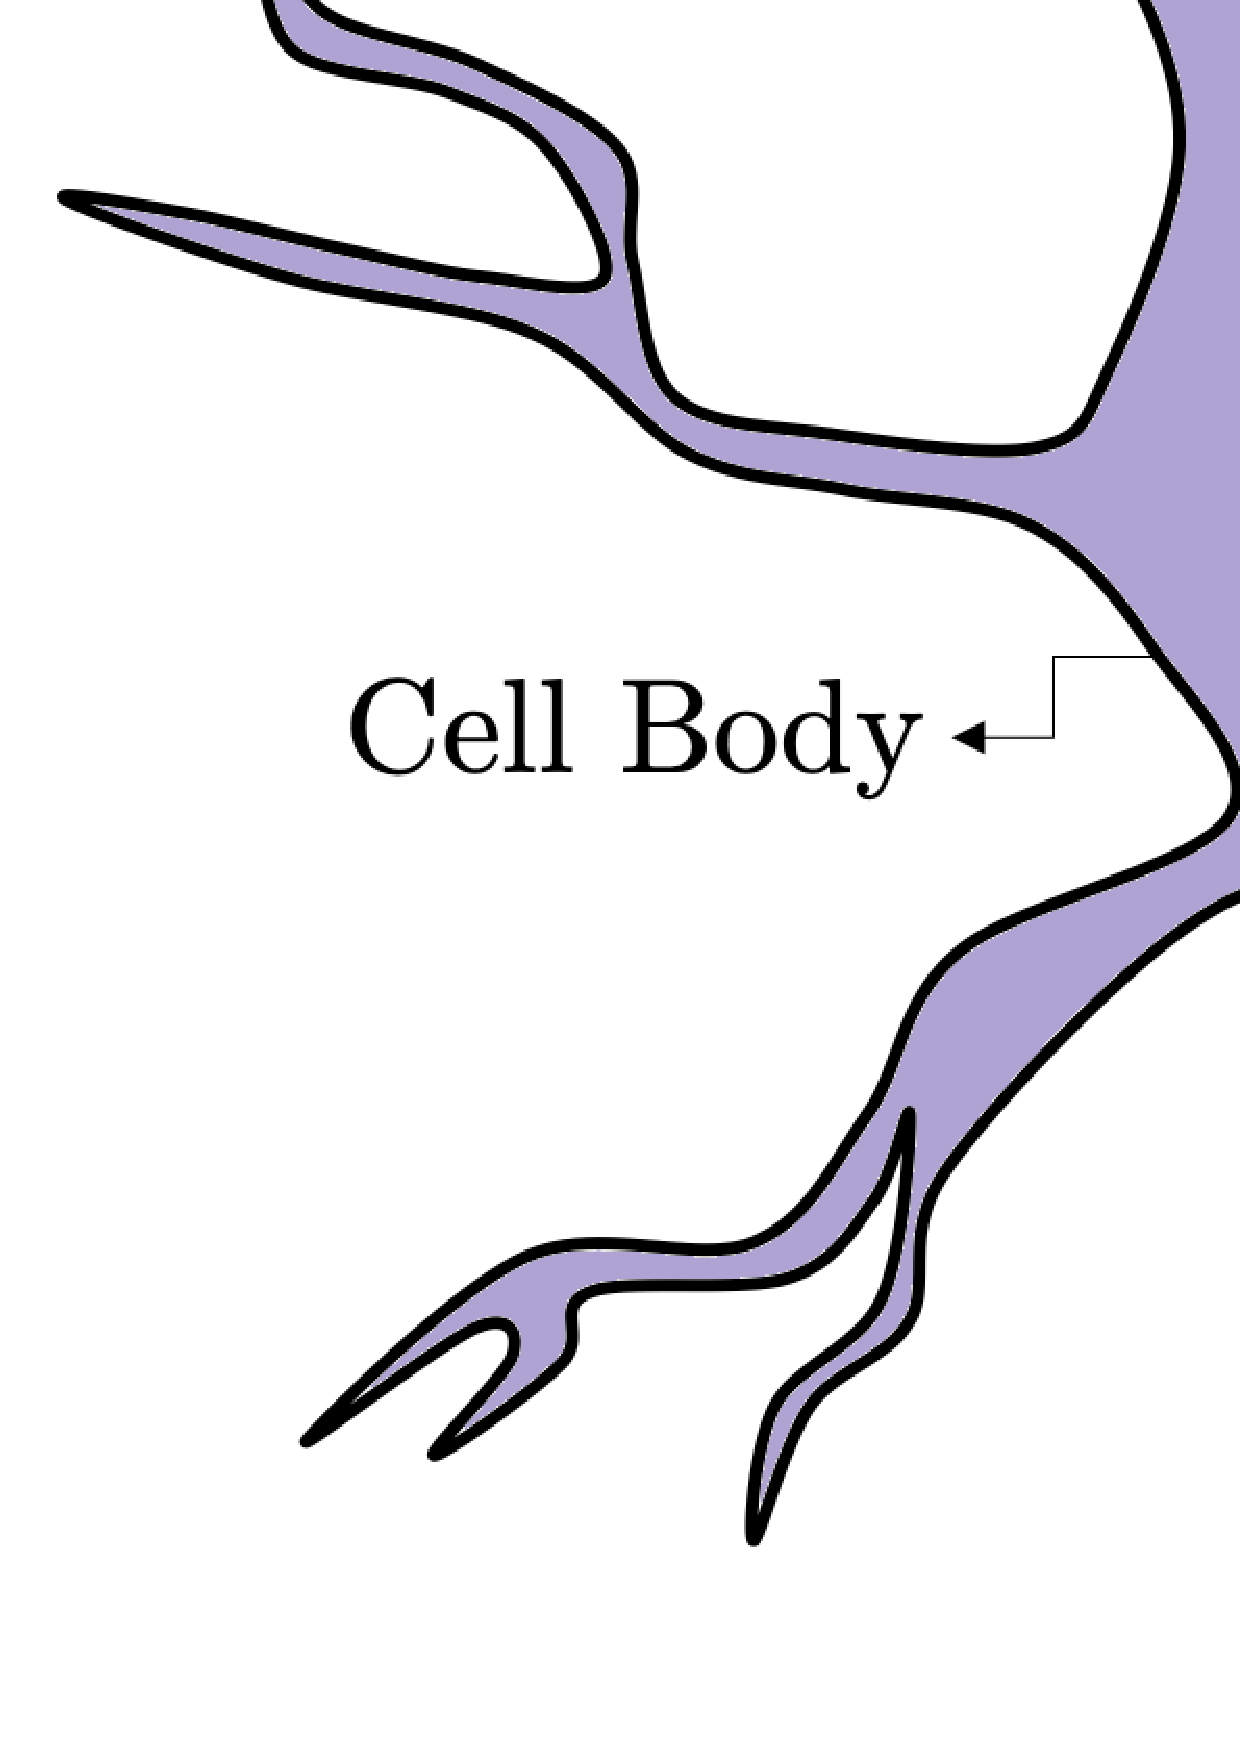
\includegraphics[width=0.95\textwidth]{biological_neuron.pdf}
      \caption[The \index{biological neuron}biological Neuron]{An illustration of the \index{biological neuron}biological Neuron.}
      \label{fig:biological_neuron}
\end{figure}

The biological neural systems are made up of microscopic nerve cells called neurons~\cite{ref:jain:1996}. Figure~\ref{fig:biological_neuron} illustrates a single \acs{BN}. The main components of the \acs{BN} include the cell body, \index{dendrites}\textit{dendrites} and the \index{axon}\textit{axon}. \Acp{NN} are formed through the connections between the \index{axon}axons and \index{dendrites}dendrites of various neurons. This is known as \index{synaptogenesis}\textit{synaptogenesis}~\cite{ref:huttenlocher:1997}. Such a connection is referred to as a \index{synapse}\textit{synapse}. Communication takes place, through the synapse, by electro-chemical pulse and is often referred to as an \textit{activation} or \textit{action potential}.  Communication signals propagate from the \index{dendrites}dendrites, through the cell body to the axon of a neuron, provoking a signal in the post-synaptic neuron~\cite{ref:engelbrecht:2007}. The greater the connection between two neurons, the stronger the communication.  Kennedy~\cite{ref:kennedy:2016} defines stronger \index{synapse}synapses as ones that contribute more depolarisation to the neural membrane upon activation than weaker ones. Stronger \index{synapse}synapses have a higher probability of generating an action potential in the post-synaptic neuron. During activation, the pre-synaptic neuron release neurotransmitters that bind to the post-synaptic neuron~\cite{ref:khanacademy:synapse}. The frequent release of these molecules cause the \index{synapse}synapse to grow. Connections that grow over time yield stronger signals (learning), while connections that are weak propagate low intensity signals and vanish over time (forgetting). The ability of synapses to strengthen and weaken over time is known as \index{synaptic plasticity}\textit{synaptic plasticity}~\cite{ref:huttenlocher:1997}.

\index{artificial neuron}
\section{Artificial Neuron}\label{sec:anns:an}

This section introduces the \acs{AN}. Brief discussion follow on the various components that make up the \acs{AN}.

The \acs{AN} implements a nonlinear mapping from $\mathbb{R}^{I}$ to
$\mathbb{R}^{T}$, usually in the ranges $[0,1]$ or $[-1,1]$, depending on the
activation function used~\cite{ref:engelbrecht:2007} and is given
as

\begin{equation}
      f_{AN} \colon \mathbb{R}^{I} \to \mathbb{R}^{T}
      \label{eq:an_function_mapping}
\end{equation}

where $f_{AN}$ is the mapping function produced by the \acs{AN}, $I$ is the total number of dimensions of the input in real-number space ($\mathbb{R}$), and $T$ is the total number of dimensions of the target (desired output) in real-number space.

The \acs{AN} implements various components and is illustrated in Figure~\ref{fig:artificial_neuron}.

\begin{figure}[htb]
      \centering
      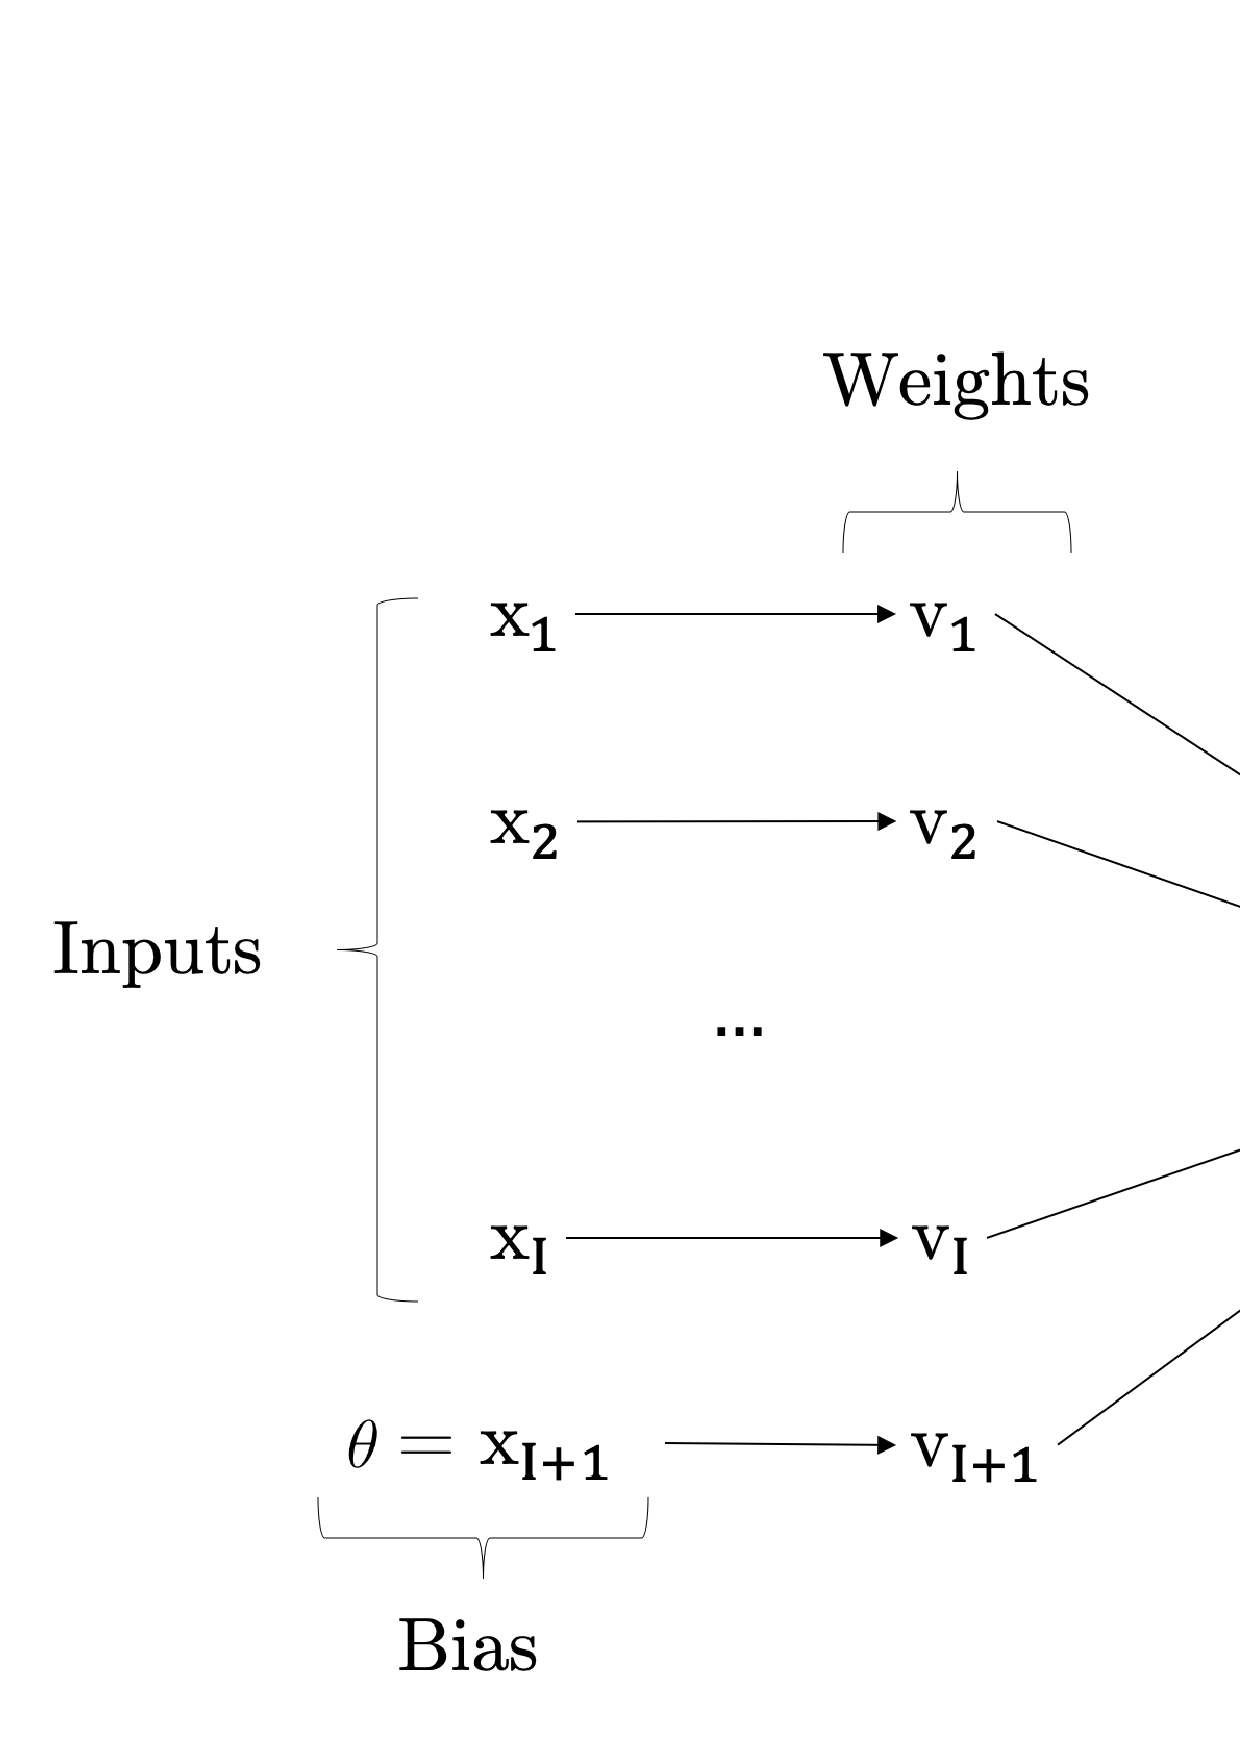
\includegraphics[width=\textwidth]{artificial_neuron.pdf}
      \caption[The \index{artificial neuron}artificial neuron]{An illustration of the \index{artificial neuron}artificial neuron.}
      \label{fig:artificial_neuron}
\end{figure}

Each of the components of the \acs{AN} is inspired by some element of the \acs{BN}. Brief descriptions of these are given as follows:

\begin{itemize}
      \item \textbf{Input:} The input models the activations received from the pre-synaptic neuron or from some environment sensor. Input is represented by the input vector $\boldsymbol{x}$, in Figure~\ref{fig:artificial_neuron}.

      \item \textbf{Weights:} The weights model the \index{synapse}synapses and connection strengths. Weights are represented by the weight vector $\boldsymbol{v}$, in Figure~\ref{fig:artificial_neuron}.

      \item \index{net input signal}\textbf{Net input signal:} The \index{net input signal}net input signal models the net resulting activations from all connected pre-synaptic neurons or environment sensors. The \index{net input signal}net input signal is represented by $net$, in Figure~\ref{fig:artificial_neuron}.

      \item \textbf{Biases:} The biases model a mechanism introduced to influence the strength of the activation (output signal) of the \acs{AN}. The bias is represented by $\theta$, in Figure~\ref{fig:artificial_neuron}.

      \item \index{activation function}\textbf{Activation function:} The activation function models the action potential of the \acs{BN} and is based on the net input signal. The \index{activation function}activation function is represented by $f$, in Figure~\ref{fig:artificial_neuron}.

      \item \textbf{Output:} The output models the activation by the post-synaptic neuron. Output is represented by the output vector $\boldsymbol{y}$, in Figure~\ref{fig:artificial_neuron}.
\end{itemize}

The following sections provide a detailed discussion on each of the above mentioned components.


\subsection{Input}\label{sec:anns:an:input}

Input signals are $I$-dimensional vectors of numerical values that are obtained either through some environment sensor or from other \acp{AN}. Input signals are often referred to as \index{features}\textit{features} or \index{independent variables}\textit{independent variables}~\cite{ref:francis:2001}. Throughout this dissertation, a single input vector is referred to as a \textit{pattern}. Input data must first be pre-processed before it is presented to the \acs{AN}. Input pre-processing techniques are presented in the following sections.


\subsubsection{Input Pre-Processing}\label{sec:anns:an:input:input_pre_processing}

Input pre-processing improves the training process and contributes to the success of the practical application of the \acs{ANN}~\cite{ref:kuzniar:2017}. The primary purpose of input pre-processing is to modify the input data so that it can better match predicted output data. There are many techniques to consider when pre-processing input data. These techniques include methods to encode data to certain formats, to scale to the correct ranges and to deal with incomplete, invalid or irrelevant data. For the purposes of this dissertation, \textit{data encoding} and \textit{normalisation} techniques are considered.


\index{encoding}
\subsubsection{Encoding}\label{sec:anns:an:input:encoding}

For qualitative data, the class labels have to be converted from textual to numerical representations. In general, class labels are encoded as numerical vectors~\cite{ref:srinidhi:2018, ref:brownlee:2017:one-hot}. One such encoding technique is referred to as \index{one-hot encoding}\textit{one-hot encoding}. Harris and Harris~\cite{ref:harris:2010} describe \index{one-hot encoding}one-hot encoding as a group of vector elements where the classes are represented with a single high element (represented by $1$) and all the others low (represented by $0$). Each element $y_k$, where $k$ is the $k$-th element of the encoded vector $\boldsymbol{y}$, uniquely refers to a class. An activation, represented by a value of $1$ at a given index thus represents a class associated with that index.

\index{normalisation}
\subsubsection{Normalisation}\label{sec:anns:an:input:normalisation}

Numerical data must be normalised and scaled appropriately for the \acs{AN}. In general, input data is normalised to a range that is appropriate for the \index{activation function}activation function being used by the \acs{AN}. Normalisation and scaling yields input data that is comparable to the output produced by the \acs{AN}. For the purposes of this disseration, the \index{min-max scaler}min-max scaler~\cite{ref:al:2006} and the \index{standard score scaler}standard score scaler~\cite{ref:jain:2005} are considered.

\index{min-max scaler}
\subsubsection{Min-Max Scaler}\label{sec:anns:an:input:min_max_scaler}

The \index{min-max scaler}min-max scaler, also called \index{unity-based normalisation}\textit{unity-based normalisation}, scales values to the range $[0,1]$. The \index{min-max scaler}min-max scaler is used as a pre-processing technique for target values when the \index{sigmoid}\textit{sigmoid} \index{activation function} activation function is used. The \index{min-max scaler}min-max scaler is given as

\begin{equation}
      x_{i,p}'  = \frac{x_{i,p} - x_{i_{min}}}{x_{i_{max}} - x_{i_{min}}}
      \label{eq:min_max_scaler}
\end{equation}

where $x_{i,p}^{'}$ is the normalised form of $x_{i,p}$, the $i$-th dimension of the input vector $\boldsymbol{x}_p$, $p \in \{1,2, \dots, P \}$, where $P$ is the total number of input patterns, $x_{i_{min}}$ and $x_{i_{max}}$ are respectfully the minimum and maximum values of the $i$-th dimension for all input vectors $\boldsymbol{x}_p$.

\index{standard score scaler}
\subsubsection{Standard Score Scaler}\label{sec:anns:an:input:standard_score_scaler}

The \index{standard score scaler}standard score scaler, also known as the \index{z-score scaler}\textit{z-score scaler}, scales values by subtracting the mean and scaling to the unit variance of each dimension $i$ for all input patterns $\boldsymbol{x}_p, p \in \{1,2, \dots, P\}$. The \index{standard score scaler}standard score scaler is used as a pre-processing technique for target values when the \index{hyperbolic tangent}\textit{hyperbolic tangent} \index{activation function}activation function\index{activation function} is used. The \index{standard score scaler}standard score scaler is given as

\begin{equation}
      x_{i,p}^{'} = \frac{x_{i,p} - \mu_i}{\sigma^2_i}
      \label{eq:standard_score_scaler}
\end{equation}

where $\mu_i$ and $\sigma^2_i$ are respectfully the mean and unit variance of the $i$-th dimension of all input vectors $\boldsymbol{x}_p$.

\subsection{Weights}\label{sec:anns:an:weights}

The connection strength that synapses in the \acs{BN} have is modeled in the \acs{AN} as weight vectors of numerical values associated with each dimension of the input. Weights can either dampen or strengthen the input by some negative or positive numerical value. Changes in the weight associated with a feature changes the influence that that particular feature has on the predicted output. Finding the correct value for each weight, such that the \acs{AN} yields optimal output, is an optimisation problem~\cite{ref:thierens:1993}. Research has shown that weight initialisation plays an important role in the efficient training of \acp{ANN}~\cite{ref:thimm:1995}.

\subsubsection{Weight Initialisation}\label{sec:anns:an:weights:initialisation}

Weight initialisation is the process by which candidate solutions (represented by the weights of the \acs{AN}) to the problem are ``placed'' in the search space. Weight initialisation influences the speed of convergence, the probability of convergence and the generalisation capabilities of \acp{ANN}~\cite{ref:fernandez:2001}. Finding the optimal initialisation values for weights is non-trivial and can be seen as another optimisation problem~\cite{ref:de:2016, ref:erdogmus:2003, ref:yam:2000}.

Weight initialisation is dependent on the \index{activation function}activation function used. If weights are initialised as values that are too small, the vanishing gradients problem can occur~\cite{ref:hanin:2018}. If weights are initialised as values that are too big, output of the activation function would not be in the active range. This leads to unit saturation, and exploding gradients can occur~\cite{ref:hanin:2018, ref:yadav:2018}.

Many different weight initialisation techniques have been developed~\cite{ref:erdogmus:2003}. Some techniques have been developed to address the problems that are mentioned above~\cite{ref:yadav:2018}. For the purposes of this dissertation, focus is put on \index{random uniform sampling}random uniform sampling, \index{Glorot uniform sampling}\textit{Glorot uniform (Xavier)} sampling and \index{Glorot normal sampling}\textit{Glorot normal} sampling~\cite{ref:glorot:2010}. Brief discussions on each of these weight initialisation techniques are presented as follows.


\index{random uniform sampling}
\subsubsection{Random Uniform Sampling}\label{sec:anns:an:weights:random_uniform_sampling}

\index{random uniform sampling}Random uniform sampling initialises weights uniformly in the range $[\omega_{min}, \omega_{max}]$, written as $w_{i} \sim \textit{U} (\omega_{min}, \omega_{max})$, where the $\omega_{min}$ and $\omega_{max}$ are respectfully the lower and upper bounds of the uniform distribution. Suggested parameter values are $(-1, 1)$ or $(-0.5, 0.5)$~\cite{ref:nguyen:1990}.


\index{Glorot uniform sampling}
\subsubsection{Glorot Uniform Sampling}\label{sec:anns:an:weights:glorot_uniform_sampling}

\index{Glorot uniform sampling}Glorot uniform sampling is a specialisation of \index{random uniform sampling}random uniform sampling, whereby $\omega = \sqrt{\frac{6}{fanin + fanout}}$ and $fanin$ is the number of input neurons to the weight vector and $fanout$ is the number of output neurons from the weight vector.

\index{Glorot normal sampling}
\subsubsection{Glorot Normal Sampling}\label{sec:anns:an:weights:glorot_normal_sampling}

\index{Glorot normal sampling}Glorot normal sampling initialises weights by sampling from a truncated normal distribution centred on a mean of $0$ and with $\sigma = \sqrt{\frac{2}{I + K}}$, where $\sigma$ is the standard deviation of the distribution. $I$ and $K$ are respectfully the number of input and output units in the weight vector. \index{Glorot normal sampling}Glorot normal sampling has been shown to decrease training time~\cite{ref:glorot:2010}.


\index{net input signal}
\subsection{Net Input Signal}\label{sec:anns:an:net_input}

\acp{AN} accumulate the net resulting input signal from all input dimensions into a value called the \index{net input signal}\textit{net input signal}, expressed as $net$. This signal is passed to the \index{activation function}activation function, which provokes an artificial action potential in the \acs{AN}.

A common way by which the \index{net input signal}net input signal is calculated is by means of \acp{SU}~\cite{ref:engelbrecht:2007}, which compute the \index{net input signal}net input signal as the weighted sum of all input signals and is given as

\begin{equation}
      net = \sum_{i=1}^{I}{x_{i}v_{i}}
      \label{eq:summation_units}
\end{equation}

where $x_{i}$ is the $i$-th dimension of the input vector $\boldsymbol{x}$, and $v_{i}$ is the $i$-th dimension of the weight vector $\boldsymbol{v}$, associated with the given input dimension.


\subsection{Biases}\label{sec:anns:an:biases}

A bias/threshold term $\theta$ is introduced to help translate the output of the \index{activation function}activation function~\cite{ref:benitez:1997}. The value of $\theta$ can be learned during the training process along with the weights of the \acs{ANN}. In order to simplify equations, the input and weight vectors are augmented such that the input and hidden layers have an additional neuron/unit, called the \textit{bias unit}~\cite{ref:engelbrecht:2007}. The net input signal can then be rewritten to consider the bias unit, leading to an augmented net input signal.


\subsubsection{Augmented Net Input Signal}\label{sec:anns:an:biases:augmented_net_input_signal}

The augmented net input signal, that includes the bias unit, has the form $net^{'} = net - \theta$, with $\theta = x_{i+1}v_{i+1}$. A constant value $x_{i+1} = -1$ can be used, meaning that the weight associated with the bias unit, $v_{i+1}$, is optimised along with the other weights during the optimisation process. The net input signal, as given in Equation~\eqref{eq:summation_units}, then changes as

\begin{equation}
      \begin{split}
            net{'} & = net - \theta \\
            & = \sum_{i=1}^{I} x_i v_i - \theta\\
            & = \sum_{i=1}^{I} x_i v_i + x_{i+1} v_{i+1} \\
            & = \sum_{i=1}^{I+1} x_i v_i
            \label{eq:augmented_vectors}
      \end{split}
\end{equation}


\subsection{Activation Functions}\label{sec:anns:an:act_functions}

An \index{activation function}activation function is used to model the action potential of the \acs{AN}~\cite{ref:ziv:1994, ref:hodgkin:1952}. The \index{activation function}activation function takes as a parameter, the augmented \index{net input signal}net input signal. When the output produced by the activation function surpasses some threshold value $\tau$, we consider that neuron to have ``fired'' an output signal. \index{activation function}Activation functions thus model \textit{phase shift}. In the context of classification problems, \index{activation function}activation functions form decision boundaries between classes. In the context of regression problems, \index{activation function}activation functions try to approximate some function that maps the input data to some target data.

In general, activation functions produce a non-linear mapping of $\mathbb{R}^{I}$ to the range $[0,1]$ or $[-1,1]$ as shown in Equations~\eqref{eq:an_function_mapping_0_1} and~\eqref{eq:an_function_mapping_minus_1_1} below.

\begin{equation}
      f_{AN}: \mathbb{R}^{I} \rightarrow [0,1]
      \label{eq:an_function_mapping_0_1}
\end{equation}

\begin{equation}
      f_{AN}: \mathbb{R}^{I} \rightarrow [-1,1]
      \label{eq:an_function_mapping_minus_1_1}
\end{equation}

Many different \index{activation function}activation functions have been developed~\cite{ref:karlik:2011}. For the purposes of this dissertation, focus is put on the \acf{ReLU}~\cite{ref:jarrett:2009, ref:nair:2010}, the \acf{LReLU}~\cite{ref:maas:2013}, the \index{sigmoid}sigmoid~\cite{ref:lecun:1988} and the \index{hyperbolic tangent}hyperbolic tangent~\cite{ref:lin:2008} \index{activation function}activation functions.


\subsubsection{Rectified Linear Unit}\label{sec:anns:an:act_functions:relu}

The \acf{ReLU} \index{activation function}activation function is an \index{activation function}activation function defined in the positive part of its argument and is given as

\begin{equation}
      f(x) = x^{+} = \max(0,x)
      \label{eq:relu}
\end{equation}

An advantage of \acs{ReLU} is that it is not susceptible to the \index{vanishing gradients problem}vanishing gradients problem~\cite{ref:xu:2015, ref:maksutov:2018} which occurs when gradients in the first layers of a multi-layer \acs{ANN} approach zero, and have no effect on the training process.


\subsubsection{Leaky Rectified Linear Unit}\label{sec:anns:an:act_functions:leaky_relu}

The \acf{LReLU} \index{activation function}activation function is a variant of the \acs{ReLU} \index{activation function}activation function that avoids zero gradients in the negative part of its argument by introducing a scaling parameter, $\alpha > 0$~\cite{ref:xu:2015}. Similar to \acs{ReLU}, \acs{LReLU} is not susceptible to the \index{vanishing gradients problem}vanishing gradients problem. However, \acs{LReLU} does not suffer from the \index{dying ReLU problem}dying \acs{ReLU} problem~\cite{ref:agarap:2018}, which occurs when the neurons that use \acs{ReLU} \index{activation function}activation functions become \textit{inactive} and only output $0$ due to a negative net input signal. The \acs{LReLU} \index{activation function}activation function is given as

\begin{equation}
      f_{AN}(net - \theta) =
      \begin{cases}
            net - \theta         & \text{if $net \geq \theta $} \\
            \alpha(net - \theta) & \text{otherwise}             \\
      \end{cases}
      \label{eq:leaky_relu}
\end{equation}

By introducing a parameter $\alpha > 0$, negative \index{net input signal}net input signals will still yield non-zero activations, resulting in non-zero gradients and avoiding gradient saturation. Non-zero gradients are required by some heuristics such as \acs{SGD} in order to be able to effectively train \acp{ANN}~\cite{ref:hanin:2018}. An illustration of \acs{LReLU} with various values for $\alpha$ and $\theta = 0$ is given in Figure~\ref{fig:anns:activation_functions:leaky_relu}.

\begin{figure}[htb]
      \centering
      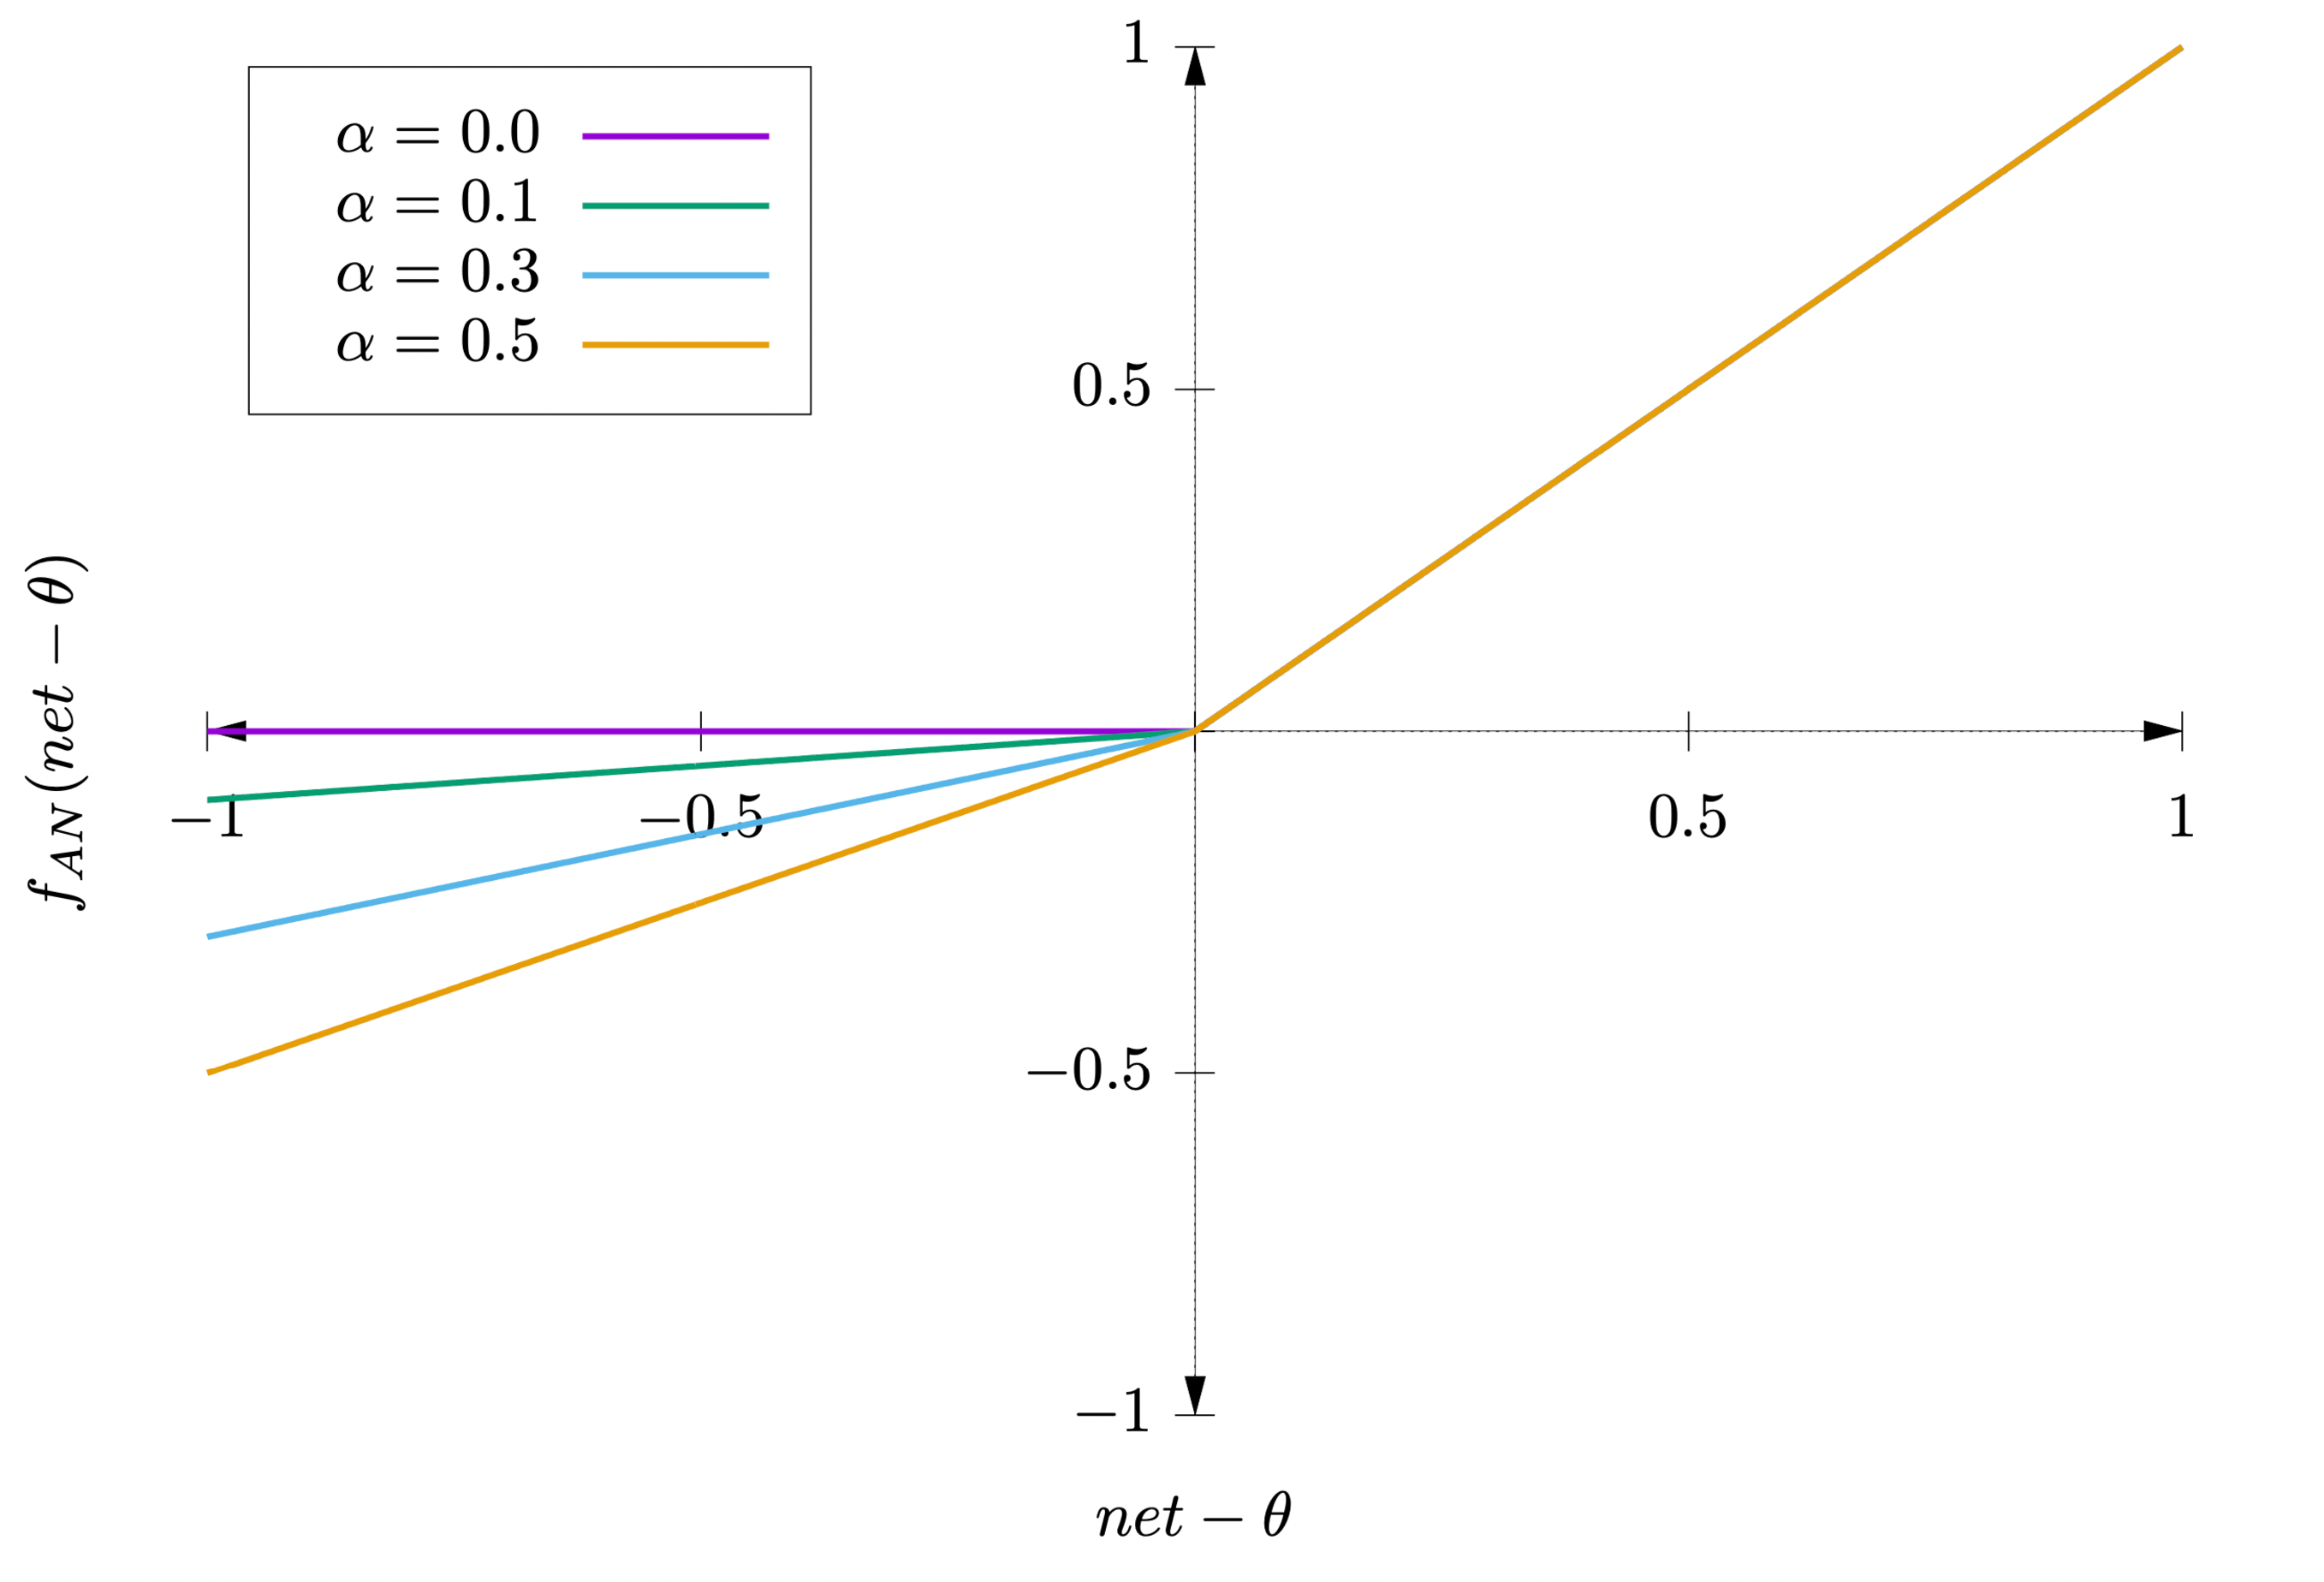
\includegraphics[width=0.75\textwidth]{lrelu.pdf}
      \caption[The \acs{LReLU} \index{activation function}activation function]{An illustration of the \acs{LReLU} \index{activation function}activation function with various values for $\alpha$ and $\theta = 0$.}
      \label{fig:anns:activation_functions:leaky_relu}
\end{figure}

\subsubsection{Sigmoid}\label{sec:anns:an:act_functions:sigmoid}

The \index{sigmoid}sigmoid activation is the continuous differentiable approximation of the step function, which was used in the original perceptron model developed by~\citeauthor{ref:rosenblatt:1957}~\cite{ref:rosenblatt:1957}, and yields output in the range $(0, 1)$. The \index{sigmoid}sigmoid \index{activation function}activation function is given as

\begin{equation}
      f_{AN}(net - \theta) = \frac{1}{1+e^{-\lambda(net - \theta)}}
      \label{eq:sigmoid}
\end{equation}

where $\lambda$ is a control parameter that controls the steepness of the sigmoid activation function and is usually set to $\lambda = 1$. An illustration of the \index{sigmoid}sigmoid \index{activation function}activation function with various values for $\lambda$ and $\theta = 0$ is given in Figure~\ref{fig:anns:activation_functions:sigmoid}.

\begin{figure}[htb]
      \centering
      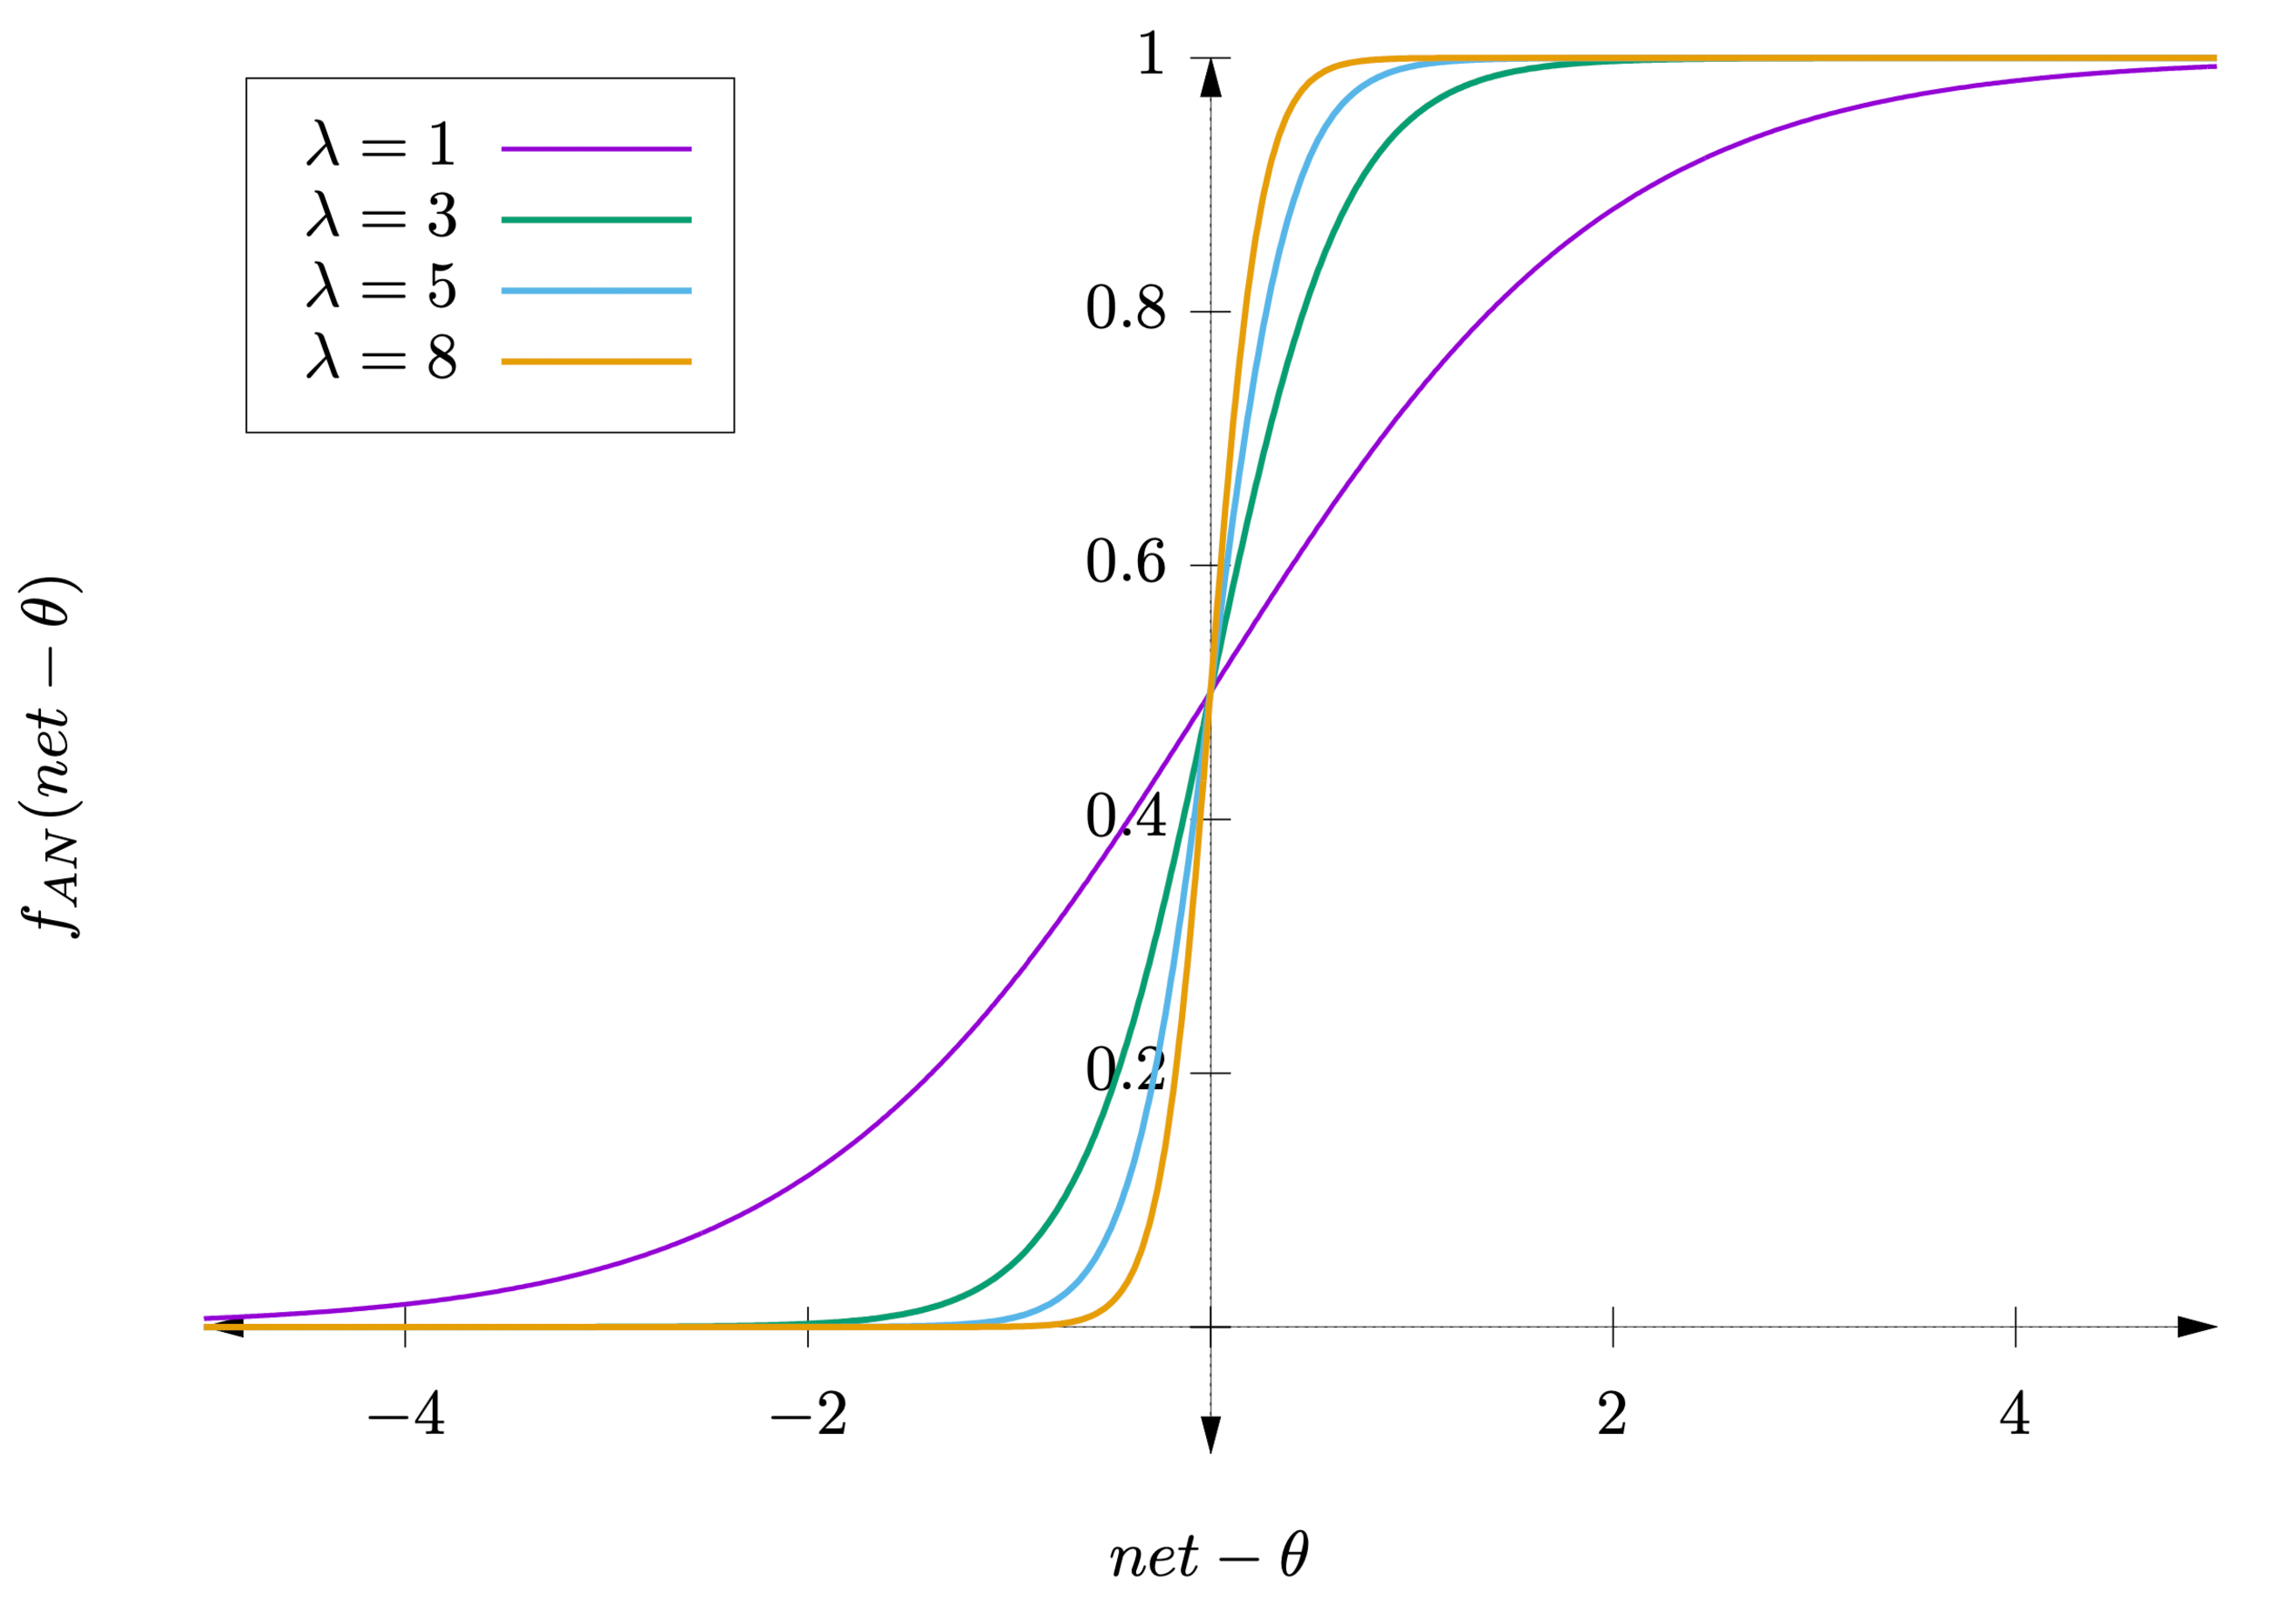
\includegraphics[width=0.75\textwidth]{sigmoid.pdf}
      \caption[The \index{sigmoid}sigmoid \index{activation function}activation function]{An illustration of the \index{sigmoid}sigmoid \index{activation function}activation function with various values for $\lambda$ and $\theta = 0$.}
      \label{fig:anns:activation_functions:sigmoid}
\end{figure}

\subsubsection{Hyperbolic Tangent}\label{sec:anns:an:act_functions:tanh}

The \index{hyperbolic tangent}hyperbolic tangent \index{activation function}activation function has a similar shape to that of the \index{sigmoid}sigmoid \index{activation function}activation function, but yields output in the range $(-1, 1)$. The \index{hyperbolic tangent}hyperbolic tangent \index{activation function}activation function is given as

\begin{equation}
      f_{AN}(net - \theta) = \frac{e^{\lambda(net - \theta)}-e^{-\lambda(net - \theta)}}{e^{\lambda(net - \theta)}+e^{-\lambda(net - \theta)}}
      \label{eq:hyperbolic_tangent}
\end{equation}

An illustration of the \index{hyperbolic tangent}hyperbolic tangent \index{activation function}activation function with various values for $\lambda$ and $\theta = 0$ is given in Figure~\ref{fig:anns:activation_functions:hyperbolic_tangent}.


\begin{figure}[htb]
      \centering
      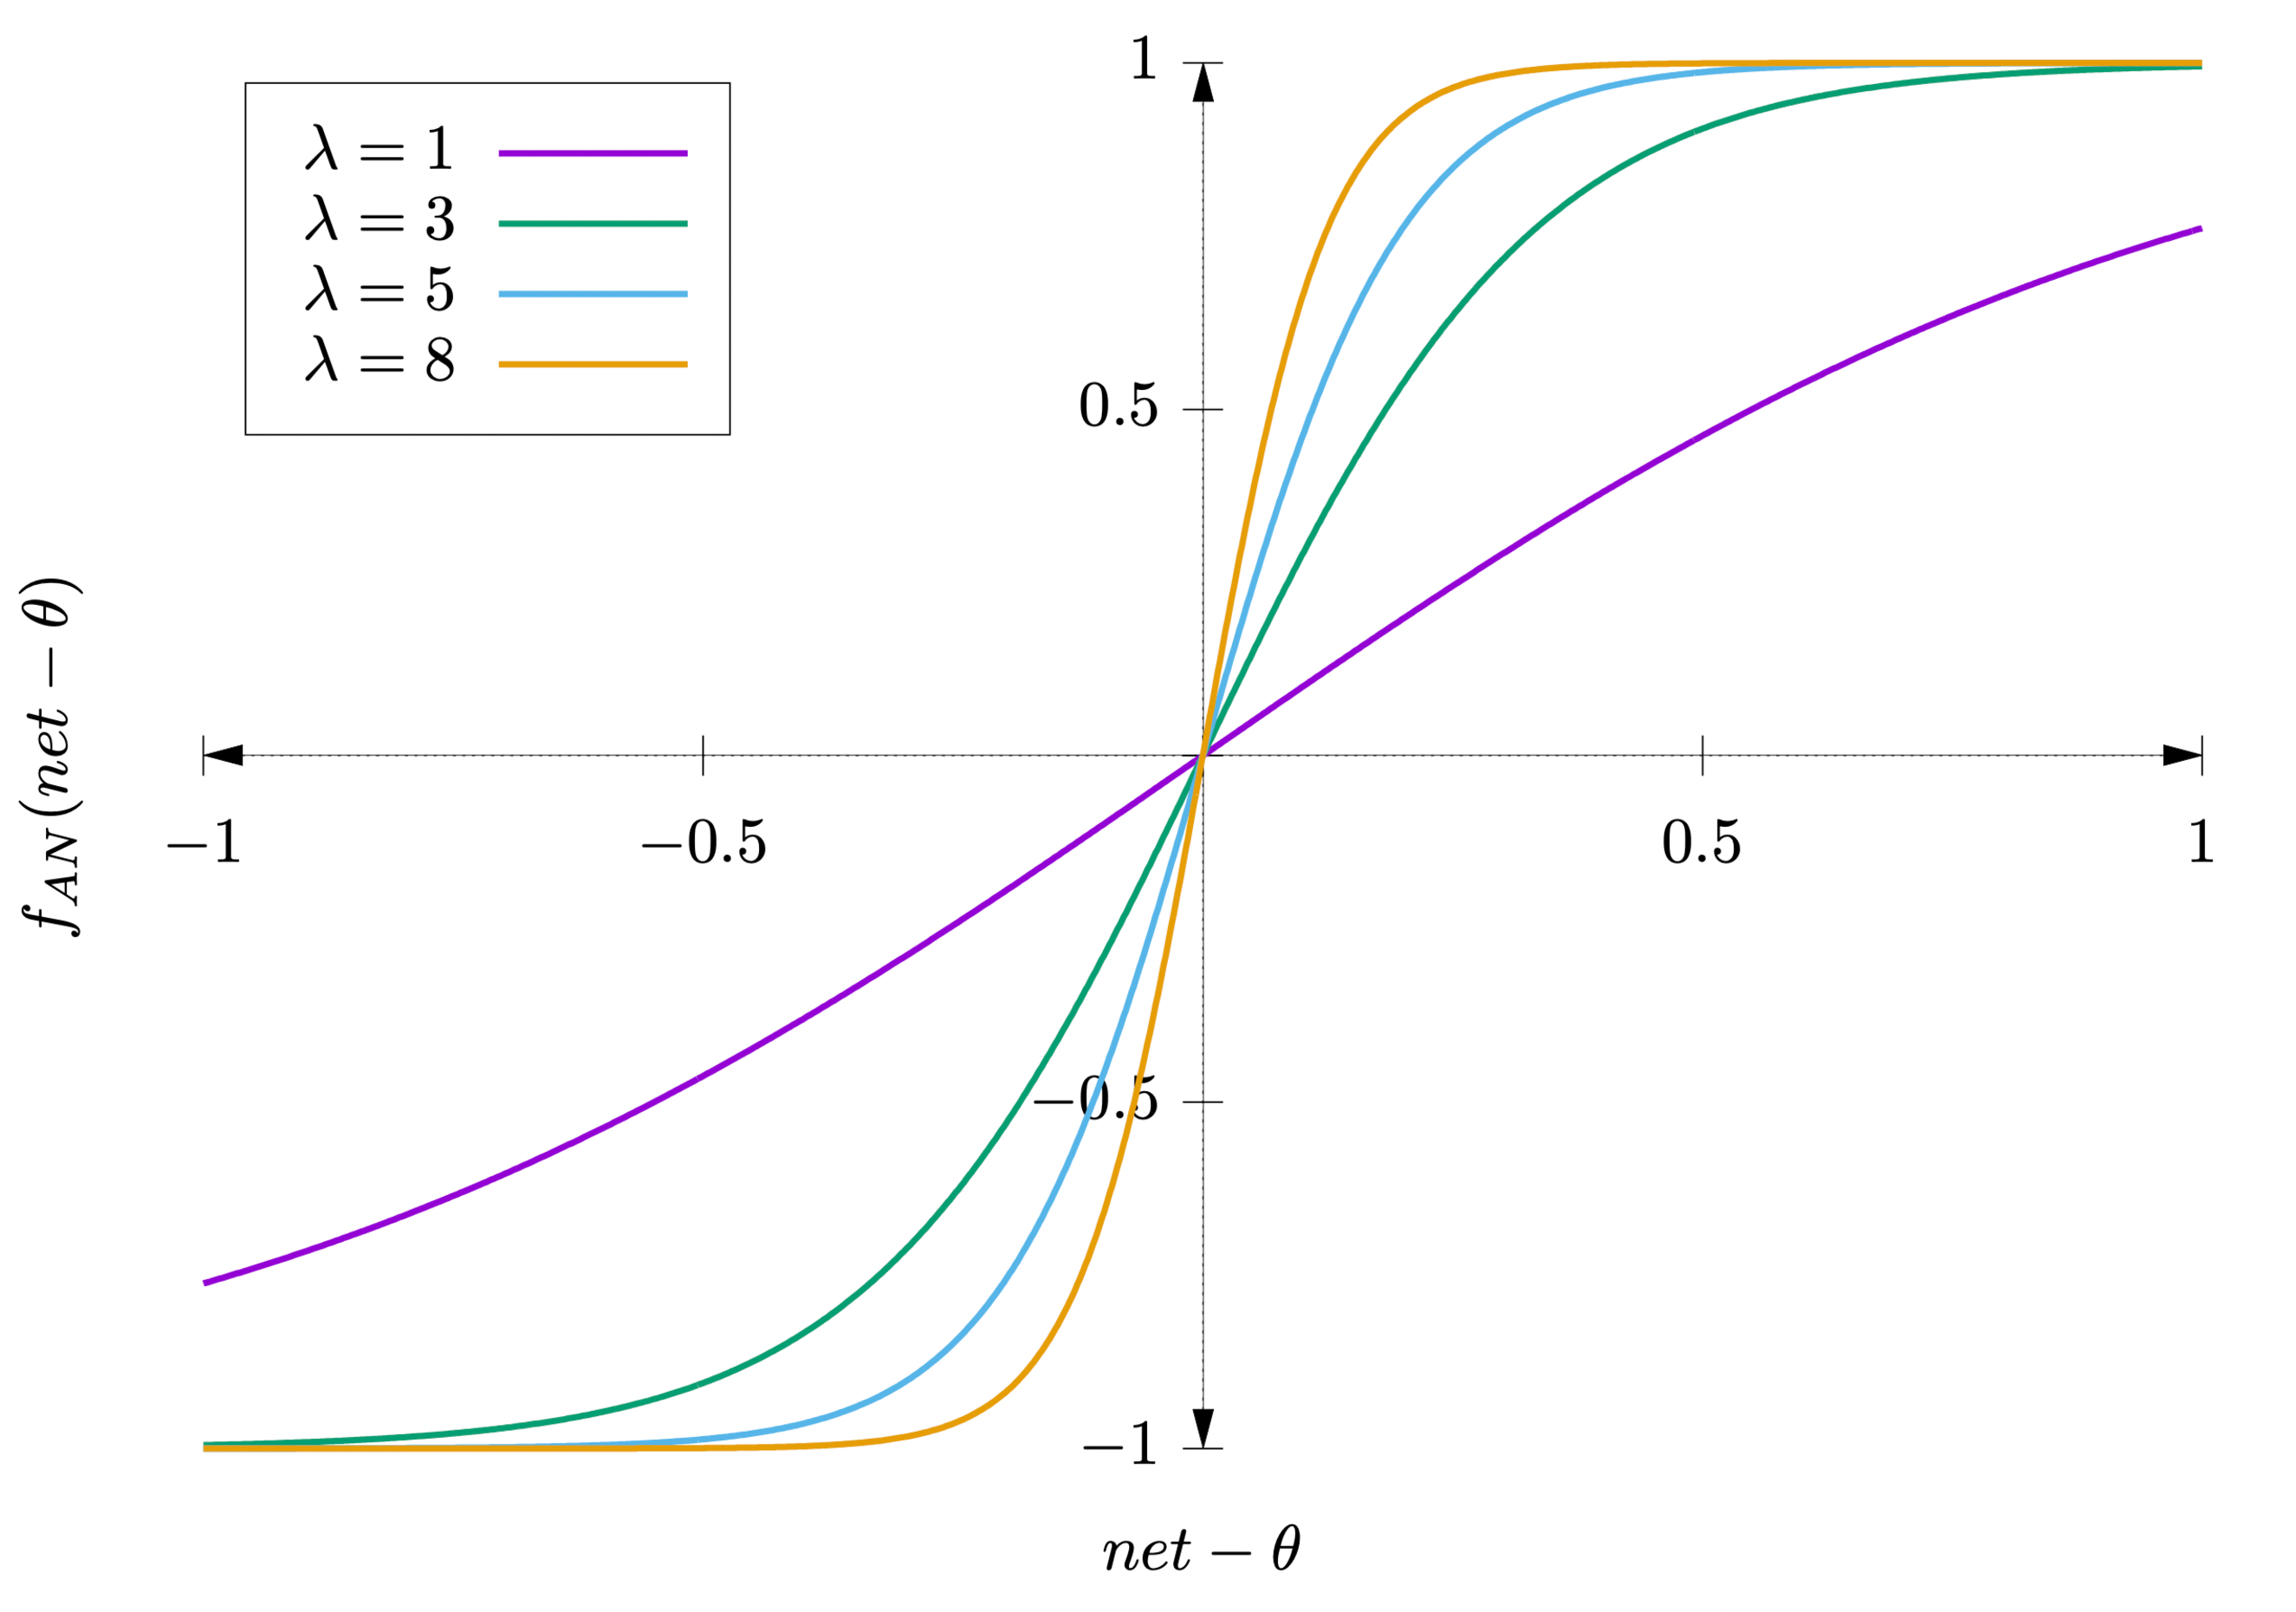
\includegraphics[width=0.75\textwidth]{tanh.pdf}
      \caption[The \index{hyperbolic tangent}hyperbolic tangent \index{activation function}activation function]{An illustration of the \index{hyperbolic tangent}hyperbolic tangent \index{activation function}activation function with various values for $\lambda$ and $\theta = 0$.}
      \label{fig:anns:activation_functions:hyperbolic_tangent}
\end{figure}


\subsection{Output}\label{sec:anns:an:output}

Output signals are numerical values that represent the output of the \acs{AN}'s \index{activation function}activation function. Output signals are often referred to as \textit{predictions}. Output values need to be post-processed to ensure the practical application of the \acs{AN}.

\subsubsection{Output Post-Processing}\label{sec:anns:an:output:output_post_processing}

Output post-processing converts output values to ranges that better match that of the target values. The post-processing techniques that are applicable depend on the type of problem (regression or classification), pre-processing techniques used, as well as the \index{activation function}activation function used. For the purposes of this dissertation, data decoding, normalisation and
re-scaling techniques are considered.


\subsubsection{Decoding}\label{sec:anns:an:output:decoding}

Data decoding refers to the process of undoing the encoding process. For min-max scaling, data is converted back to the range $(x_{min}, x_{max})$. In the context of an \acs{AN}, binary logistic regression problems map the output to the positive or negative class, usually separating the class decision boundary using a threshold value $\tau$. In the context of multiple \acp{AN}' output, the output is a vector of numerical values. The one-hot encoded output is then decoded by mapping the index of the output vector that yields the highest activation (argmax) to its associated class.

\subsubsection{Softmax}\label{sec:anns:an:output:softmax}

The \index{softmax}softmax function, also known as the \index{softargmax}\textit{softargmax}~\cite[p.~184]{ref:goodfellow:2016} or \index{normalised exponential function}\textit{normalised exponential function}~\cite{ref:bishop:2006} is a generalisation of the logistic function that converts a $K$-dimensional output vector $\boldsymbol{y}$ into a $K$-dimensional output vector $\boldsymbol{y^{'}}$ where each element $y^{'}_k$ is in the range $(0,1)$ and all elements sum up to $1$ as is shown in Equation~\eqref{eq:sum_after_softmax} below.

\begin{equation}
      \boldsymbol{y^{'}} \colon \mathbb{R}^{K} \to \left\{\boldsymbol{y^{'}} \in \mathbb{R}^{K} \vert y^{'}_k \in (0,1), \sum_{k=1}^{K} y_k = 1\right\}
      \label{eq:sum_after_softmax}
\end{equation}

The softmax function is then given as

\begin{equation}
      y^{'}_k = \frac{e^{y_k}}{\sum_{k = 1}^{K}e^{y_k}}
      \label{eq:softmax}
\end{equation}


\subsubsection{Argmax}\label{sec:anns:an:output:argmax}

The \index{argmax}argmax function is similar to the \index{softmax}softmax function, with the difference that the element $y_k, k \in \{1,2, \dots, K\}$ with the highest output value is set to $1$ and the rest are set to $0$. All elements still sum to $1$, but the activation is only observed at index $k$ where the activation is $1$. The \index{argmax}argmax function is given as

\begin{equation}
      y^{'}_k =
      \begin{cases}
            1 & \text{if $y_k = \max(y_1, y_2, \dots, y_K)$} \\
            0 & \text{otherwise}
            \label{eq:argmax}
      \end{cases}
\end{equation}

Figure~\ref{fig:anns:activation_functions:softmax_argmax} illustrates the comparison of transformations of the output vector $\boldsymbol{y}$, where the \index{sigmoid}sigmoid, the \index{softmax}softmax and the \index{argmax}argmax \index{activation function}activation functions are used.


\begin{figure}[htb]
      \centering
      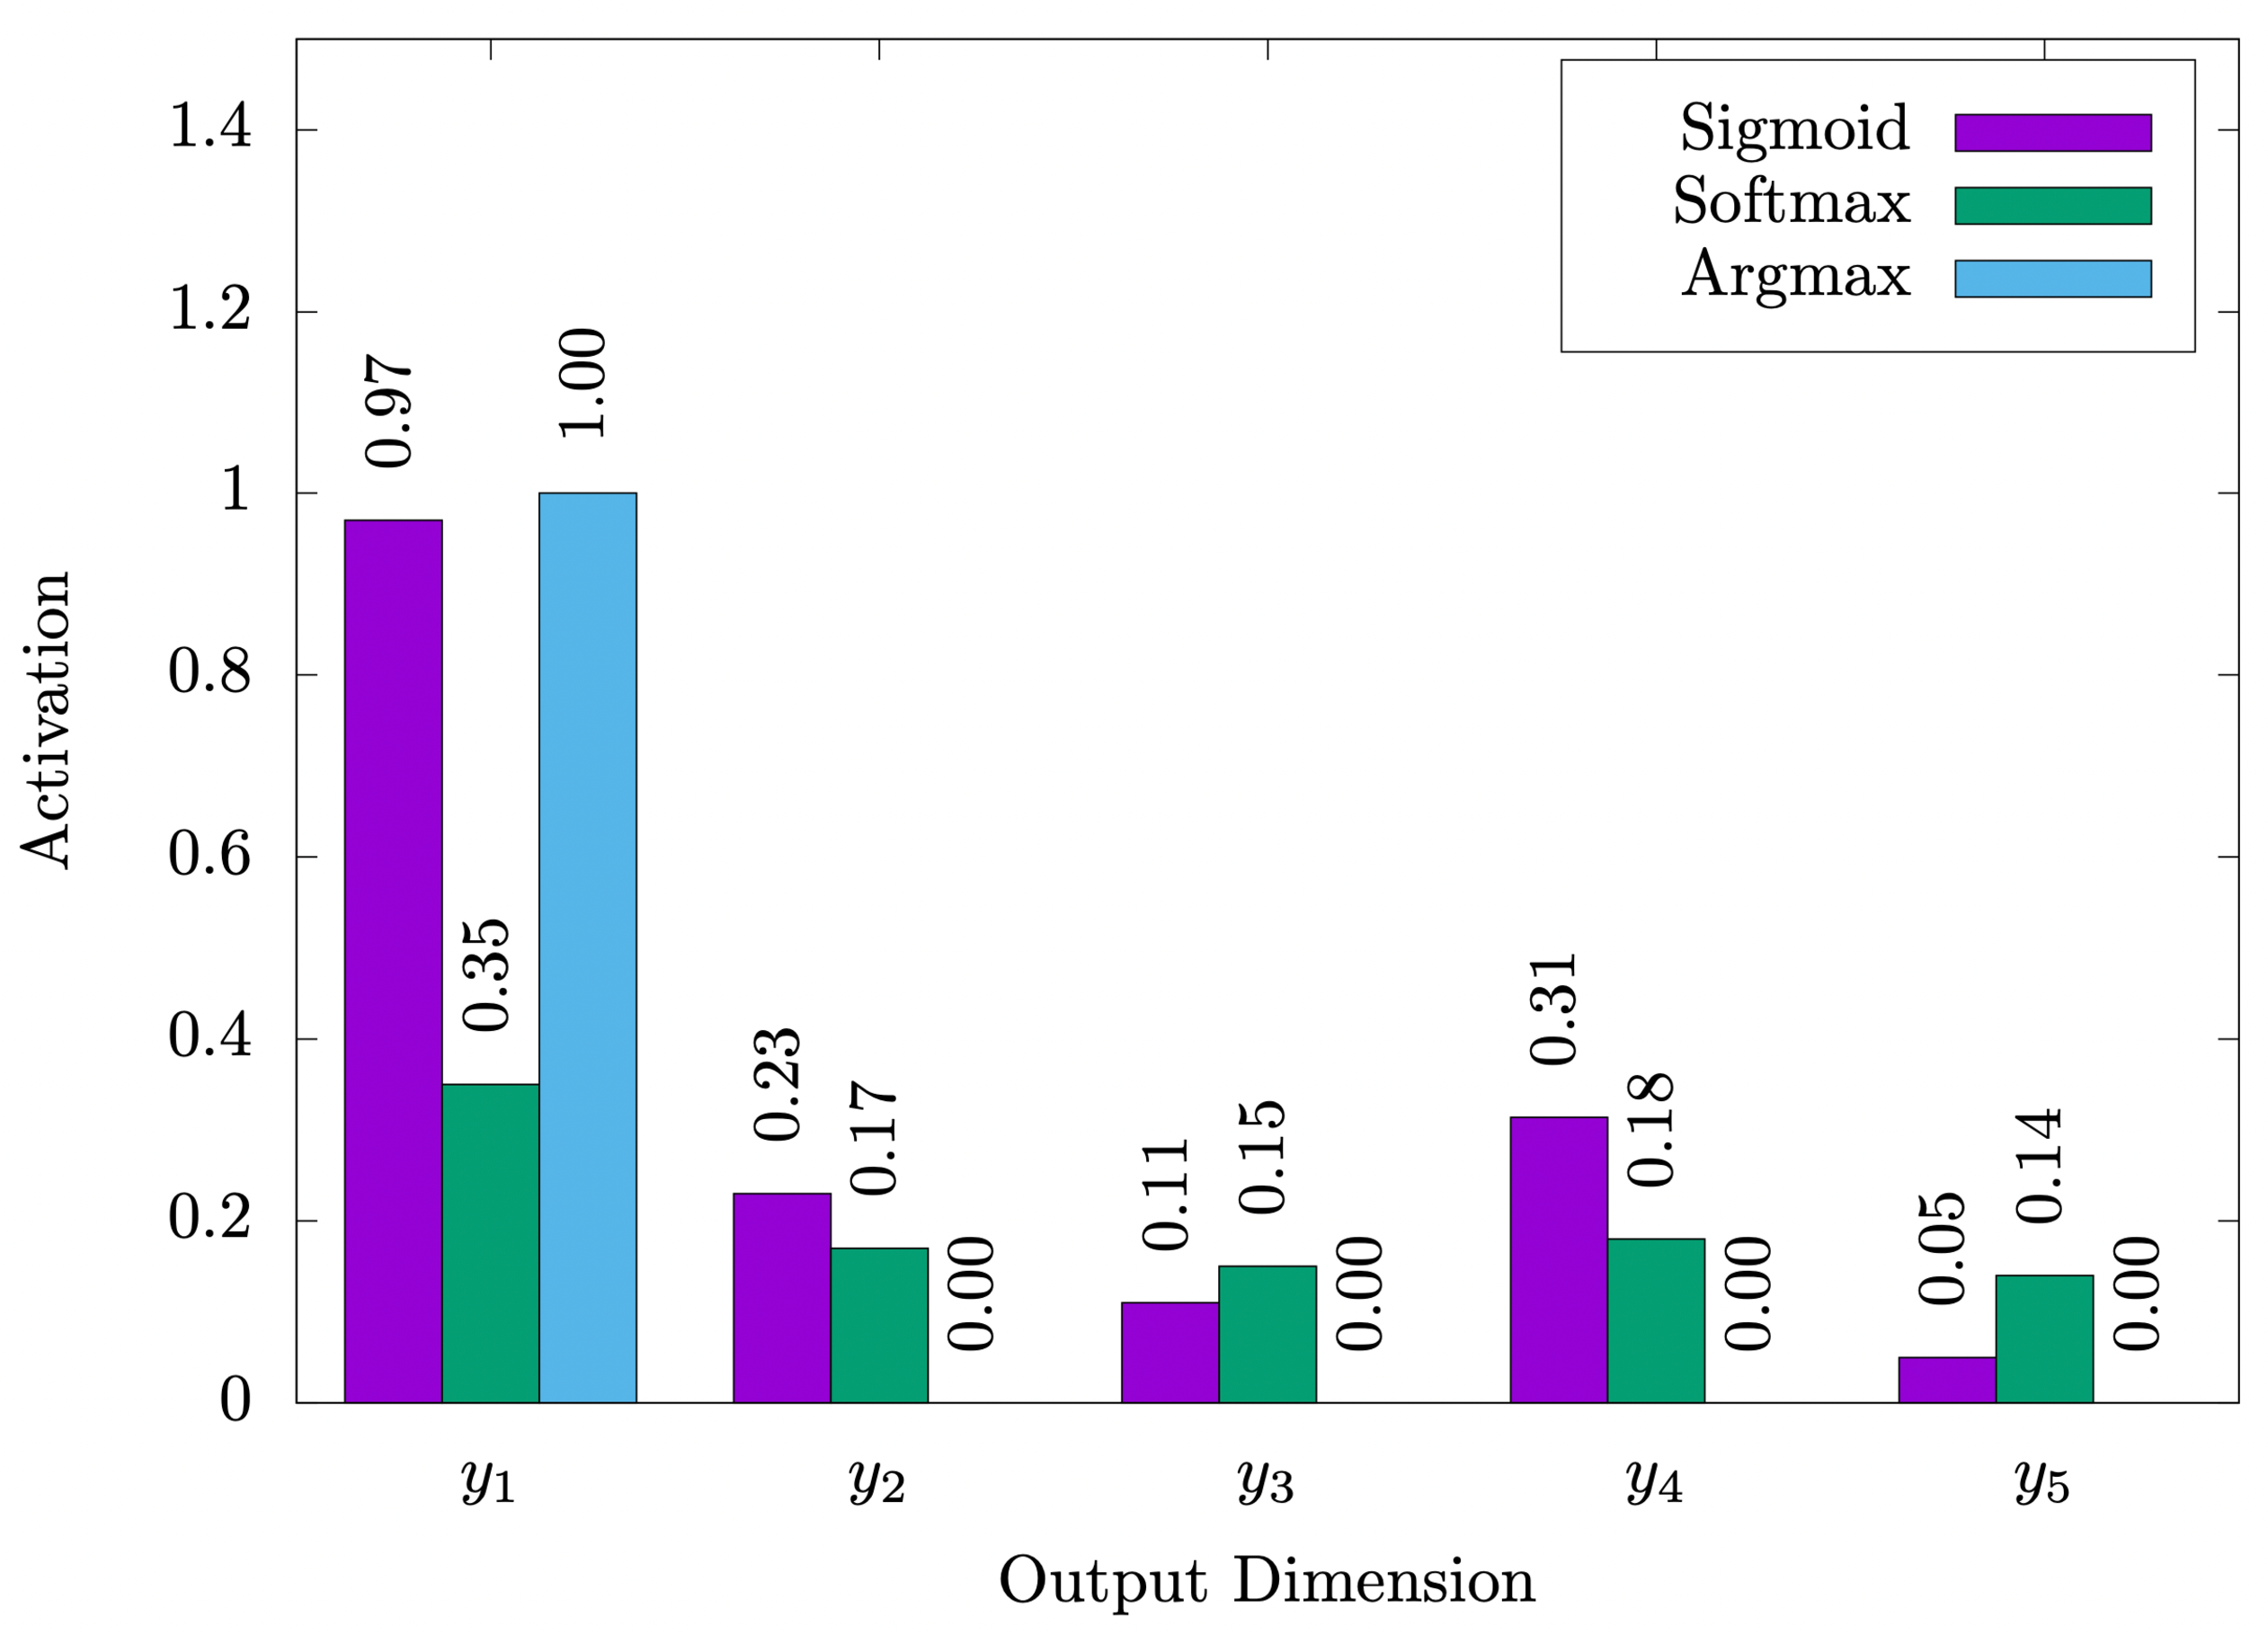
\includegraphics[width=0.65\textwidth]{output_modifiers.pdf}
      \caption[The results of \index{softmax}softmax and \index{argmax}argmax]{An illustration of \index{softmax}softmax and \index{argmax}argmax applied after the \index{sigmoid}sigmoid \index{activation function}activation function.}
      \label{fig:anns:activation_functions:softmax_argmax}
\end{figure}


\section{Artificial Neural Network} \label{sec:anns:ann}

Multiple \acp{AN} can be organised and used together forming a ``network'' of \acp{AN} referred to as an \acf{ANN}. This section presents \acp{ANN} and discussions follow on their applications, architecture, and topologies. Specific reference is made to \acf{FFNN}, a specific type of \acs{AN} used in this dissertation.

\subsection{Applications} \label{sec:anns:anns:applications}

\acp{ANN} are inspired by the biological brain. Our brains model biological neural networks with neuron counts in the hundreds of billions and synapse counts in the trillions. To emulate the computational capability of the human brain is not yet possible on modern day hardware.~\citeauthor{ref:sandberg:2008}~\cite{ref:sandberg:2008} approximates a computational requirement of 256 000 terabytes/s to emulate the entire brain. Despite our shortage in hardware capabilities, \acp{ANN} have been successfully applied to a range of problem classes.~\citeauthor{ref:engelbrecht:2007}~\cite{ref:engelbrecht:2007} summarises some common problems that are solved using \acp{ANN} and can be listed as follows.

\begin{itemize}
      \item \textbf{Classification}: Predicting the class of an input vector~\cite{ref:khan:2001}.

      \item \textbf{Pattern Matching}: Producing closely associated patterns based on an input vector~\cite{ref:cannady:1998, ref:kumar:1994}.

      \item \textbf{Pattern Completion}: Completing the missing parts of an input vector~\cite{ref:dayhoff:2001}.

      \item \textbf{Optimisation}: Producing optimal values of parameters in a optimisation problems~\cite{ref:specht:1991}.

      \item \textbf{Data Mining}: Feature discovery in large datasets~\cite{ref:singh:2009}.
\end{itemize}

The composition of \acp{AN} in an \acs{ANN} is expressed as the \textit{architecture} and \textit{topology} of the \acs{AN}. The exact composition to use depends on the problem being solved.

\subsection{Architecture} \label{sec:anns:anns:architecture}

The architecture of the \acs{ANN} refers to the way in which \acp{AN} are organised. \acp{ANN} can be organised in layers where a single layer can contain multiple \acp{AN}. Generally, each layer makes use of the same \index{activation function}activation function. Output from one layer is propagated as input to the next layer. This dissertation focuses on the simplest architecture, containing three particular layers, including the input, hidden and output layers. \acp{ANN} with this type of architecture are usually referred to as \textit{shallow} \acp{NN}. A description of each layer is given as follows.

\subsubsection{Input Layer}\label{sec:anns:anns:architecture:input}

The input layer contains the input data to the \acs{ANN}. Since the input layer simply provides the input data, some literature do not consider the input layer as an actual part of the \acs{ANN}~\cite{ref:engelbrecht:2007}.

\subsubsection{Hidden Layer}\label{sec:anns:anns:architecture:hidden}

The hidden layer contains a collection of ``hidden'' \acp{AN}, also referred to as \textit{hidden units} or \textit{nodes}. Hidden units are used if the target data is not linearly separable~\cite{ref:engelbrecht:2007}. It has been shown that \acp{ANN} that incorporate monotonically increasing differentiable \index{activation function}activation functions can approximate any continuous function with just one hidden layer, given that the hidden layer has enough hidden units~\cite{ref:hornik:1989}.

\subsubsection{Output Layer}\label{sec:anns:anns:architecture:output}

The output layer contains the final activations or the predictions of the \acs{ANN}. These outputs can be used to measure the performance of the \acs{ANN}.


\subsection{Topology}
\label{sec:anns:anns:topology}

The topology of the \acs{ANN} refers to the way that layers of \acp{AN} are connected to each other. There are many different topologies~\cite{ref:miikkulainen:2010}. For the purposes of this dissertation focus is put on a \index{fully connected topology}\textit{fully connected} topology where each \acs{AN} in one layer is connected to all \acp{AN} in the next, without any cycles~\cite{ref:zell:1994}.


\subsection{Feedforward Neural Networks}\label{sec:anns:anns:ffnns}

\acp{FFNN} were the first and simplest type of \acp{ANN} developed~\cite{ref:schmidhuber:2015} and implement input, hidden and output layers by arranging them in sequential order. Furthermore, \acp{FFNN} implement \index{fully connected topology}fully connected topologies. In \acp{FFNN}, information moves forward, in one direction, from the input nodes, through the hidden nodes and finally to the output nodes. Depending on the optimisation algorithm used, error correction information can be ``backpropagated'' through the network. An illustration of a \acs{FFNN} is given in Figure~\ref{fig:ffnn} below.

\begin{figure}[htb]
      \centering
      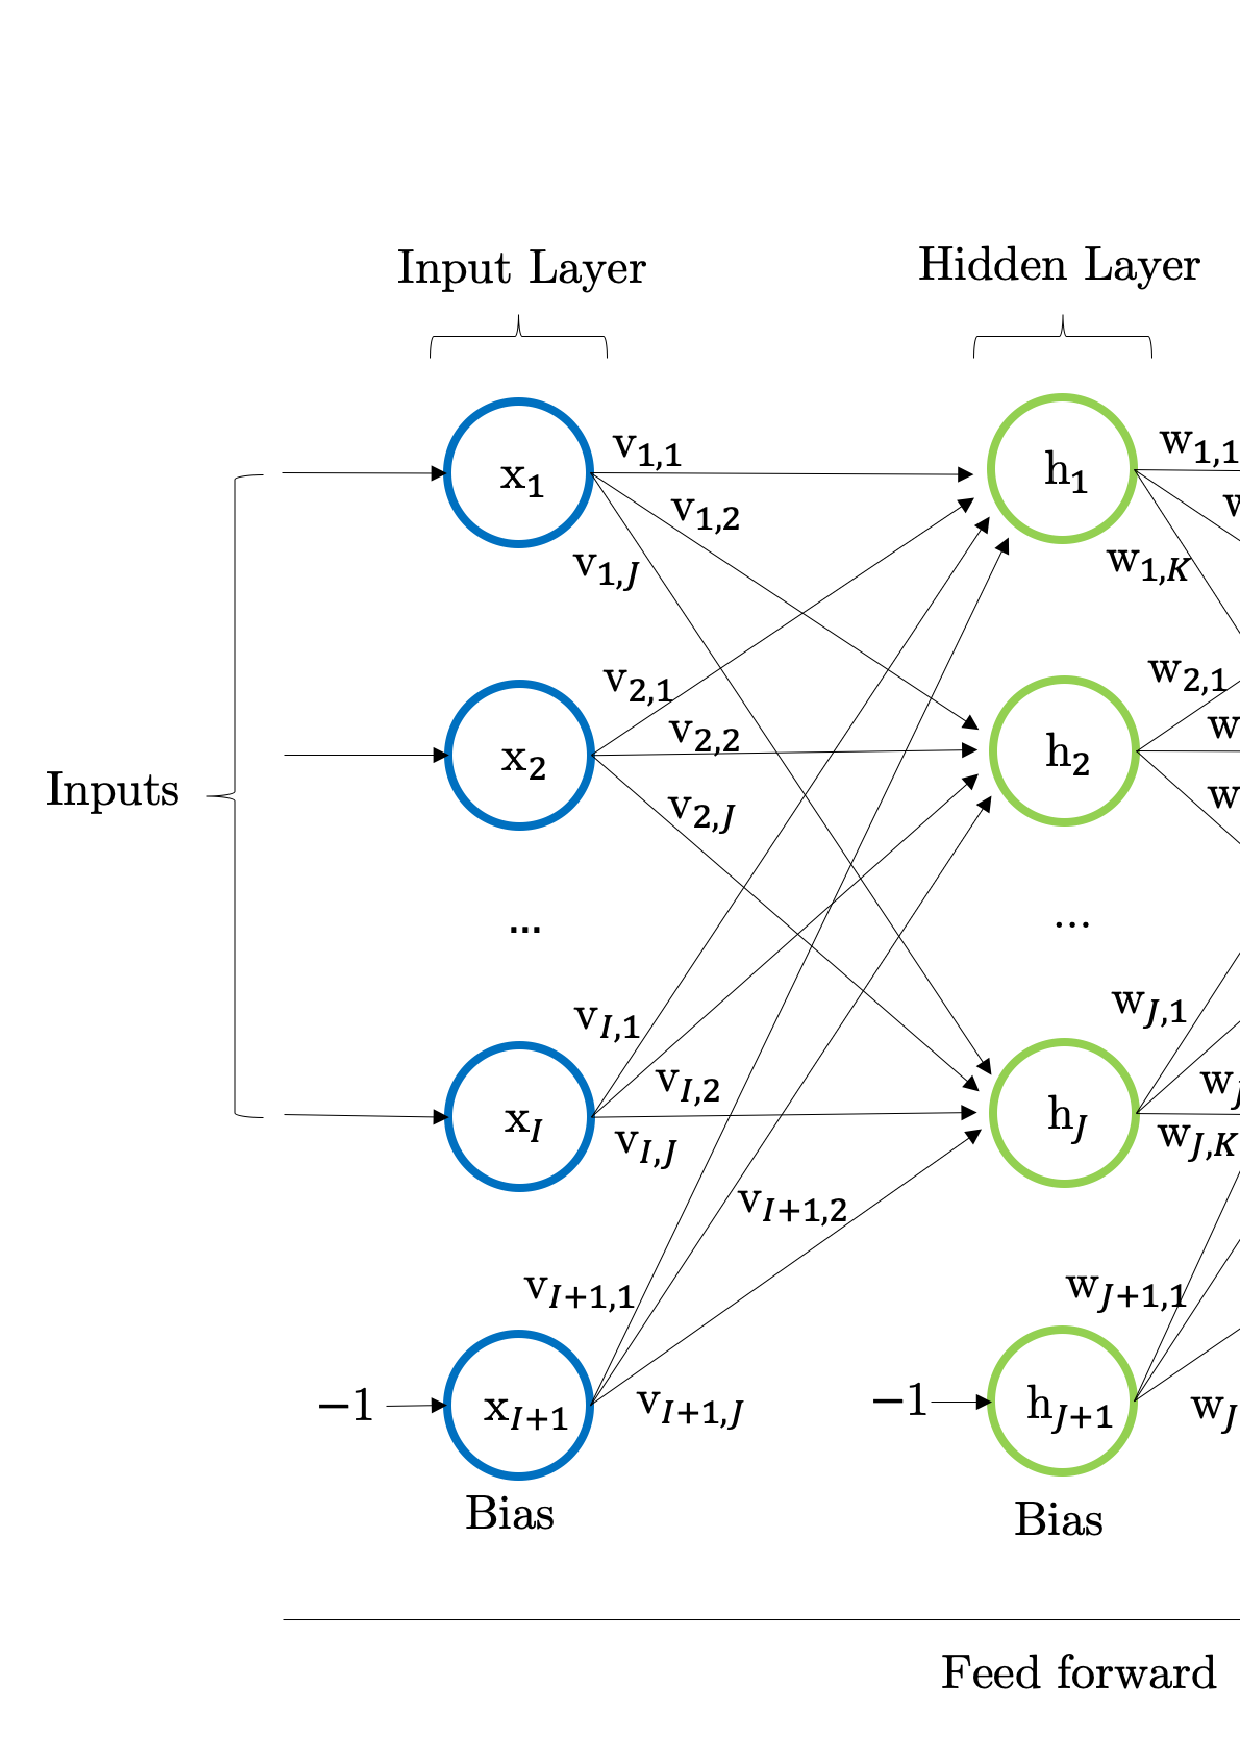
\includegraphics[width=0.98\textwidth]{feedforward_neural_network.pdf}
      \caption[A \index{feedforward neural network}feedforward neural network]{An illustration of a \index{feedforward neural network}feedforward neural network implementing input, hidden and output layers using a fully connected topology.}
      \label{fig:ffnn}
\end{figure}

In Figure~\ref{fig:ffnn}, $x_i$ refers to the $i$-th dimension in the input vector $\boldsymbol{x}$, $h_j$ refers to the $j$-th dimension in the hidden layer, $y_k$ refers to the $k$-th dimension in the output vector $\boldsymbol{y}$, $v_{i,j}$ refers to the weight associated with input node $x_i$ and the hidden node $h_j$, and $w_{j,k}$ refers to the weight associated with hidden node $h_j$ and the output node $y_k$.

Assuming the use of \acp{SU} and bias weights, the output for the \acs{FFNN} at index $k$, denoted $y_k$, is calculated as

\begin{equation}
      \label{eq:ffnn}
      \begin{split}
            y_k &= f\left(net_{h,y}\right) \\
            &= f\left(\sum_{j=0}^{J+1} h_j w_{j,k}\right) \\
            &= f\left(\sum_{j=0}^{J+1} f\left(net_{i,h}\right) w_{j,k}\right) \\
            &= f\left(\sum_{j=0}^{J+1} f\left(\sum_{i=0}^{I+1} x_i v_{i,j}\right) w_{j,k}\right) \\
      \end{split}
\end{equation}

The remainder of this dissertation makes use of \acp{FFNN} and is sometimes referred to as \textit{the model}.


\section{Training}
\label{sec:anns:training}

Details on the training of \acp{FFNN} are presented in this section along with
detailed discussions on \index{supervised learning}supervised learning and loss functions.

\textit{Training} is the process whereby the weights of the \acs{FFNN} are systematically changed with the aim of improving the \textit{performance} of the \acs{FFNN}. During the training process, the \acs{FFNN} is exposed to data while trying to produce some target outcome.

The degree to which the produced outcome differs from the target outcome is referred to as \textit{loss}. Since training of \acp{FFNN} is an optimisation problem, the goal of the training process is to minimise the loss of the \acp{FFNN} as it related to input and target data.

Finding the optimal weights that produce the best performance on a given task is an optimisation problem. The optimisation algorithm used to find the optimal weights is referred to as a \index{heuristic}\textit{heuristic}. \index{heuristic}Heuristics search for possible solutions in the solution-space and make use of information from the search space to guide to process.


\subsection{Supervised Learning}
\label{sec:anns:training:supervised_learning}

\index{supervised learning}Supervised learning is the process of training where the data that is presented to the \acs{FFNN} during training, includes the desired solution~\cite{ref:geron:2017}.  The \acs{FFNN} learns the mapping function from the input to the target output~\cite{ref:brownlee:2016}. The desired solutions are referred to as \textit{labels}. \index{supervised learning}Supervised learning can be used for both classification and regression problems.

The training data that is used during supervised learning, is split proportionally into a \textit{training} and \textit{validation} set. Data in the training set is used to train the \acs{FFNN}~\cite{ref:james:2013} and update the weights, while the validation dataset is used for hyper-parameter tuning, where the parameters of the training process are altered, but not the weights of the \acs{FFNN}.

Exposing the \acs{FFNN} to all training data once is referred to as an
epoch. The \acs{FFNN} is trained until some stopping condition is reached. Once the stopping condition has been reached, the \textit{performance} of the \acs{FFNN} is evaluated. The performance is directly related to the loss of the \acs{FFNN} as it relates to a \textit{test dataset}. The test dataset is a collection of data that is not used during training and is used to determine the generalisation capabilities of the \acs{FFNN} as it relates to unseen data. Overfitting and underfitting describe two possible outcomes of the training process.


\subsubsection{Overfitting}\label{sec:anns:training:process:overfitting}

\index{overfitting}Overfitting describes a scenario where the trained \acs{FFNN} performs well on training data, but does not generalise well to never before seen data from the test set~\cite{ref:tetko:1995, ref:geron:2017}. Geron~\cite{ref:geron:2017} describes \index{overfitting}overfitting as the case where \acs{FFNN} is too complex relative to the noisiness of the training data.

\subsubsection{Underfitting}\label{sec:anns:training:process:underfitting}

Underfitting describes a scenario where the \acs{FFNN} is not able to effectively learn the underlying structure of the training data~\cite{ref:tetko:1995, ref:geron:2017}. Geron~\cite{ref:geron:2017} describe underfitting as the case where the \acs{FFNN} is too simple relative to the underlying structure of the training data.\\
\\
There are two types of supervised learning algorithms based on when weights are updated~\cite{ref:engelbrecht:2007}. These include stochastic training and batch
training.


\subsubsection{Stochastic Training}\label{sec:anns:training:stochastic}

\index{stochastic training}Stochastic training, also known as \index{online learning}\textit{online learning}, is a \index{supervised learning}supervised learning variation whereby weights are adjusted after each training pattern presented. \index{stochastic training}Stochastic training benefits from shuffling data in the training dataset before presenting it to the \acs{FFNN}, in order to avoid overfitting or memorising the order in which patterns are presented~\cite{ref:engelbrecht:2007}. It has been shown that shuffling the training data can speed up convergence
\cite{ref:bengio:2012}.


\subsubsection{Batch Training}\label{sec:anns:training:batch}

\index{batch training}Batch training, also known as \index{offline learning}\textit{offline learning}, is a supervised training variation whereby weight changes are accumulated and used to adjust the weights only once, after all the training patterns have been presented.


\subsubsection{Mini-Batch Training}\label{sec:anns:training:mini_batch}

Research suggests a trade-off between stochastic and batch training by making use of mini-batches~\cite{ref:bengio:2012}. Mini-batch training is similar to batch training, however weights are updated after $\beta$ patterns have been presented, where $\beta$ is the mini-batch size.\\
\\
Performance metrics are used during training on the training set and evaluation on the test set. There are many different performance measurements that can be used, however this dissertation focuses on performance measures related to loss. Loss is calculated using an error function. The following section presents the reader with more detail on the error functions that can be used during the training process.

\subsection{Error Functions}\label{sec:anns:training:error_functions}

This dissertation focuses on a number of error functions, including \acf{SSE}, \acf{MSE}, \acf{RMSE}, \acf{MAE}, \acf{BinXE}, \acf{CatXE} and \acf{SparseCatXE}.


\subsubsection{Sum Squared Error}\label{sec:anns:training:error_functions:sse}

The \acs{SSE} is given as

\begin{equation}
      \epsilon = \sum_{p=1}^P \sum_{k=1}^K (\hat{y}_{k,p} - y_{k,p})^2
      \label{eq:sse}
\end{equation}

where $\hat{y}_{k,p}$ is $k$-th dimension of the target output of pattern $p$, $y_{k,p}$ is $k$-th dimension of the predicted output vector $\boldsymbol{y}_{p}$ for pattern $p$, $P$ is the number of patterns in the mini-batch, and $K$ is the number of dimensions in the output vector $\boldsymbol{y}$.


\subsubsection{Mean Squared Error}\label{sec:anns:training:error_functions:mse}

The \acs{MSE} is given as

\begin{equation}
      \epsilon = \frac{\sum_{p=1}^P \sum_{k=1}^K (\hat{y}_{k,p} - y_{k,p})^2}{PK}
      \label{eq:mse}
\end{equation}


\subsubsection{Root Mean Squared Error}\label{sec:anns:training:error_functions:rmse}

The \acs{RMSE} is given as

\begin{equation}
      \epsilon = \sqrt{\frac{\sum_{p=1}^P \sum_{k=1}^K (\hat{y}_{k,p} - y_{k,p})^2}{PK}}
      \label{eq:rmse}
\end{equation}


\subsubsection{Mean Absolute Error}\label{sec:anns:training:error_functions:mae}

The \acs{MAE} is given as

\begin{equation}
      \epsilon = \frac{\sum_{p=1}^P \sum_{k=1}^K |\hat{y}_{k,p} - y_{k,p}|}{PK}
      \label{eq:mae}
\end{equation}


\subsubsection{Binary Cross-Entropy}\label{sec:anns:training:error_functions:bin_xe}

\acs{BinXE} is used in classification problems, where there are only two classes in the target output data. \acs{BinXE} is given as

\begin{equation}
      \epsilon = -\frac{\sum_{p=1}^P \sum_{k=1}^K (\hat{y}_{k,p} \log{(y_{k,p})} + (1 - \hat{y}_{k,p})\log{(1 - y_{k,p})})}{PK}
      \label{eq:bin_xe}
\end{equation}


\subsubsection{Categorical Cross-Entropy}\label{sec:anns:training:error_functions:cat_xe}

\acs{CatXE} is used in classification problems where the target output or \textit{label} is a one-hot encoded vector. \acs{CatXE} is given as

\begin{equation}
      \epsilon = -\frac{\sum_{p=1}^P \sum_{k=1}^K \sum_{c=1}^C (\mathbbm{1}_{\hat{y}_{k,p} \in C_c} \log{(y_{k,p} \left[ y_{k,p} \in C_c \right])})}{PK}
      \label{eq:cat_xe}
\end{equation}
where $\mathbbm{1}$ is the indicator function that the $k$-th index observation belongs to the $c$-th class. $C$ is the total number of unique class labels. If $C = 2$, then \acs{BinXE} can be used instead.

\subsubsection{Sparse Categorical Cross-Entropy}\label{sec:anns:training:error_functions:sparse_cat_xe}

\acs{SparseCatXE} error function is similar to \acs{CatXE} with the only difference being that the target output or label is a one-hot embedding of a class represented as an integer, $c \in \{1,2, \dots, C\}$.


\section{Summary}\label{sec:anns:summary}

This chapter presented background information on the \acs{BN}. The \acs{AN} was introduced and discussions followed on the various components that make up the \acs{AN}. Details on input, weights and biases, \index{net input signal}net input signal, \index{activation function}activation functions, and output were provided. The \acs{ANN} was introduced. \acs{ANN} design was described in terms of architecture and topologies. Special emphasis was put on \acp{FFNN}. Background information on the training of \acp{FFNN} was presented. A variant of training, called \index{supervised learning}supervised learning was presented and led to discussions on datasets, performance measures and training outcomes. The chapter concluded with a number or error functions that can be used to calculate the loss in the context of supervised learning.

\chapter{Heuristics}\label{chap:heuristics}

\begin{quotation}
      \noindent ``It is not the strongest of the species that survives. It is also not the most intelligent that survives. It is the one that is the most adaptable to change.''
\end{quotation}
\begin{flushright}
      Charles Darwin
\end{flushright}

\noindent
Many different techniques have been used to train \acp{FFNN} \cite{ref:kingma:2014}. Finding the best technique to use to train an \acs{FFNN} has been shown to be problem dependent in many cases \cite{ref:kheiri:2017}. Every technique has its characteristics, constraints, advantages and disadvantages. At the time of writing, the majority of work that is published around the training of \acp{FFNN}, involves the use of gradient-based techniques \cite{ref:nel:2021}. Gradient-based techniques are not without flaws and can, for example, yield slow convergence or get trapped in local optima \cite{ref:mingguang:2009}. Other techniques have also been used to successfully train \acp{FFNN}, including meta-heuristics such as \acf{PSO} \cite{ref:rakitianskaia:2012, ref:vanwyk:2014}, \acf{DE} \cite{ref:espinal:2011} and \acfp{GA} \cite{ref:gupta:1999}.

Chapter~\ref{chap:anns} briefly introduced the reader to the concept of \index{heuristic}\index{heuristic}heuristics and \index{meta-heuristic}meta-heuristics. This chapter presents more detailed background information on various different \index{heuristic}heuristics that have been used to train \acp{FFNN}. Broadly speaking, this chapter focuses on two different groups of \index{heuristic}heuristics, including classical gradient-based approaches and population-based \index{meta-heuristic}meta-heuristics. Each technique is presented and discussed in detail. Pseudo-code algorithms are provided for each technique and discussions follow on advantages, disadvantages, capabilities and limitations. The remainder of this chapter is structured as follows.

\begin{itemize}
      \item \textbf{Section~\ref{sec:heuristics:optimisation}} provides a brief review of optimisation. It is shown that training of \acp{FFNN} is an optimisation problem.

      \item \textbf{Section~\ref{sec:heuristics:what_is_a_heuristic}} provides background information on the origins and definition the term \index{heuristic}\textit{heuristic}. It is shown that \index{heuristic}heuristics are a class of algorithms that are used to solve optimisation problems.

      \item \textbf{Section~\ref{sec:heuristics:gd}} presents the reader with seven low-level, gradient-based \index{heuristic}heuristics, including \acf{SGD}, \acf{Momentum}, \acf{NAG}, \acf{Adagrad}, \acf{RMSProp}, \acf{Adadelta} and \acf{Adam}.

      \item \textbf{Section~\ref{sec:heuristics:mh}} presents the reader with three different population-baed \index{meta-heuristic}meta-heuristics, including \acf{PSO}, \acf{DE} and \acfp{GA}.

      \item \textbf{Section~\ref{sec:heuristics:summary}} provides the reader with a brief summary of the chapter.
\end{itemize}

\section{Optimisation}\label{sec:heuristics:optimisation}

Optimisation is the task of finding a solution to a given problem that is better than alternative solutions. Better stated by Oldewage \cite{ref:oldewage:2017}, optimisation is the task of finding values for a set of variables such that some measure of optimality is satisfied given a set of constraints. Engelbrecht \cite{ref:engelbrecht:2007} breaks optimisations problems down into three components:

\begin{itemize}
      \item An \textbf{objective function}: Represents the quantity to be optimised and is used as the ``measure of optimality''. Optimisation can be defined in terms of the minimisation or maximisation of the objective function $f$.

      \item A \textbf{set of unknowns or independent variables}: Affects the outcome of the objective function $f$ and is denoted as $x$. $f(x)$ is thus the quantification of the objective function over the unknowns, represented by $x$. Note that $x$ could be a scalar value, a vector or a matrix and notation is left out for simplicity.

      \item A \textbf{set of constraints}: Restrict and limit the values that can be assigned to the unknowns, represented by $x$. Optimisation problems that must adhere to a set of constraints are referred to as \acfp{CSP}.
\end{itemize}

\noindent
Optimisation problems come in a wide variety, and can be defined in terms of the number of variables used (uni- vs. multivariate), the number of objective functions used (single- vs. multi-objective), the degree of linearity (linear vs. quadratic/polynomial), the number of optima (uni- vs. multi-modal), the nature of the environment (static vs. dynamic), the types of variables used (separable vs. inseparable, discrete vs. continuous) and the set of constraints that the solution must adhere to (constrained vs unconstrained).

Optima can be defined as \textit{local} or \textit{global} optima. Local optima is the best optimisation of $f(x)$ in a neighbourhood of solutions, while the global optima is the best optimisation of $f(x)$ over all solutions in the solution space.

As stated in Chapter~\ref{chap:anns}, the training of an \acp{FFNN} is a particular type of optimisation problem, where the goal is to find the configuration of \textit{weights}, such that the \ac{FFNN} yields output that minimises some loss function. The mechanism by which the optimal weights for a \acs{FFNN} is sough out, is executed by an \index{optimisation algorithm}optimisation algorithm known as a \index{heuristic}heuristic. Discussions on the details of heuristics are presented in the following sections.

\section{What is a heuristic?}\label{sec:heuristics:what_is_a_heuristic}

The term \textit{heuristic} comes from the Latin word \textit{heuristicus} which means ``to find out or discover''. \citeauthor{ref:romanycia:1985} \cite{ref:romanycia:1985} provides a complete study on the history and origins of the term \index{heuristic}\textit{heuristic}. From their research, a proposal is made to define \index{heuristic}heuristics in the context of \ac{AI}, as any device, be it a program, rule, piece of knowledge, which is added to a problem-solving system, in expectation that on average, the performance will improve.

In the context of this dissertation, a \index{heuristic}heuristic refers to an algorithmic search technique that serves as a guide to a search process where good solutions to a optimisation problem is being sought out. Different \index{heuristic}heuristics make use of different information during the search process \cite{ref:kheiri:2017}. During the training of \acp{FFNN}, \index{heuristic}heuristics such as gradient-based \index{heuristic}heuristics make use of the derivatives obtained by evaluating the \ac{FFNN}. It can thus be said that gradient-based \index{heuristic}heuristics make use of information directly from the \textit{search space}. On the contrary, \index{heuristic}heuristics such as \index{hmeta-euristic}meta-heuristics make use of meta-information obtained as a result of evaluating the \ac{FFNN} \cite{ref:blum:2003}. The meta-information that \index{meta-heuristic}meta-heuristics make use of could include ranked-performance of a population of candidate solutions, referred to as \textit{entities}. \index{meta-heuristic}Meta-heuristics are useful when there is imperfect information about the search space \cite{ref:bianchi:2009}, and are generally less problem-specific than other classes of \index{heuristic}heuristics \cite{ref:blum:2003}. This disseration takes a particular interest in gradient-based \index{heuristic}heuristics and \index{meta-heuristic}meta-heuristics. Each of these are presented in detail in the following sections.


\section{Gradient-Based Heuristics}\label{sec:heuristics:gd}

Gradient-based \index{heuristic}heuristics are optimisation techniques that make use of derivates obtained from evaluating the model being optimised. Specifically, in the context of a minimisation problem, these techniques are called \acf{GD} heuristics as they \textit{minimise} some loss function. \Acs{GD} is generally attributed to Cauchy \cite{ref:lemarechal:2012}, who first suggested it in 1847. In 1907 Hadamard \cite{ref:hadamard:1908} independently proposed a similar method.

Although \acs{GD} \index{heuristic}heuristics where not the first \index{heuristic}heuristics used to train \ac{FFNN}
\cite{ref:engelbrecht:2007}, they are certainly the most whidely used. \Acs{GD} heuristics have become increasingly popular partly due to their simplicity and low computational overhead compared to other \index{heuristic}heuristics such as \index{meta-heuristic}meta-heuristics and other second-order derivative methods such as Newtons' method. There are many variants of \acs{GD} \index{heuristic}heuristics, however, they all fundamentally apply the same generic \acs{GD} framework called \acl{BP}.

\subsection{Backpropagation}\label{sec:heuristics:gd:backpropagation}

Chapter~\ref{chap:anns} introduced the reader to \index {supervised learning}supervised learning and presented a number of loss functions. In the context of supervised learning, loss functions produce a scalar value $\epsilon$, that represents the error between the output of the \ac{FFNN} and the desired output. When using \acs{GD} to train \acp{FFNN}, the \index{loss function}loss function is used to adjust the weights of the \ac{FFNN} in order to minimise the error \cite{ref:engelbrecht:2007}. \citeauthor{ref:engelbrecht:2007} \cite{ref:engelbrecht:2007} states that training of \acp{FFNN} using \acs{GD}, is done by calculating the gradient of $\epsilon$ in \textit{weight-space}, and then moving the weight vector along the negative gradient. An illustration of \acs{GD} is given in Figure~\ref{fig:heuristics:gd:gd_illustration}.

\begin{figure}[htbp]
      \centering
      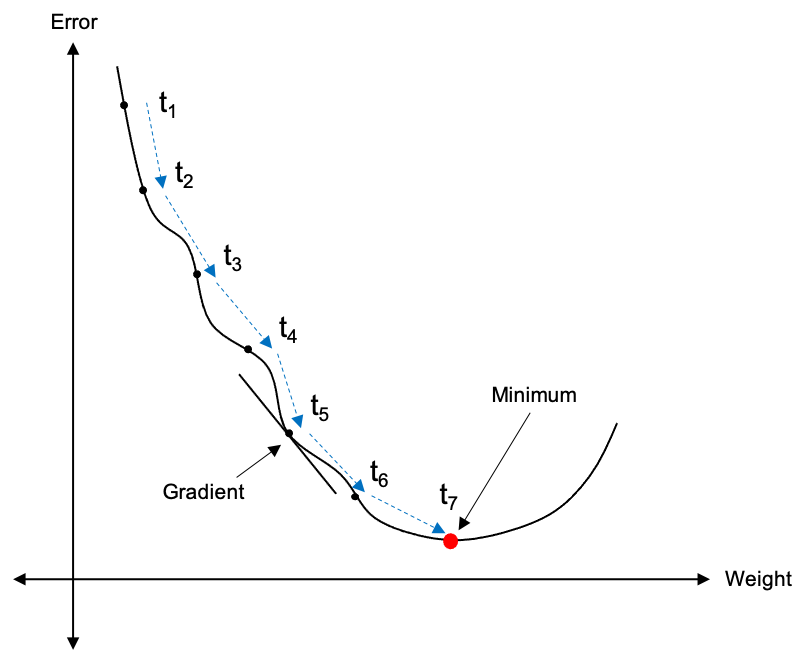
\includegraphics[width=0.85\textwidth]{images/gradient_descent.pdf}
      \caption{An illustration of \ac{GD} over various timesteps showing the minimisation of the error with regards to weight value.}
      \label{fig:heuristics:gd:gd_illustration}
\end{figure}

\noindent
The update step for \ac{GD} can be formulated as is shown in Equation~\eqref{eq:heuristics:gd:update_step_part_1} below.

\begin{equation}
      \label{eq:heuristics:gd:update_step_part_1}
      w_{i}(t) = w_{i}(t-1) + \Delta w_{i}(t)
\end{equation}

\noindent
In Equation~\eqref{eq:heuristics:gd:update_step_part_1} above, the delta weight $\Delta w$, at index $i$ and timestep $t$ is given by Equation~\eqref{eq:heuristics:gd:update_step_part_2} below.

\begin{equation}
      \label{eq:heuristics:gd:update_step_part_2}
      \Delta w_{i}(t) = -\eta\frac{\partial \epsilon}{\partial w_{i}}
\end{equation}

\noindent
In Equation~\eqref{eq:heuristics:gd:update_step_part_2} above, $\eta$ is the learning rate. The learning rate is an important hyper-parameter in gradient-based \index{heuristic}heuristic as it controls the step-size that is taken in the direction of the negative gradient at each timestep. Assuming the use of \acs{SSE} as the loss function, the partial derivative of $\epsilon$, relative to the weight $w$, at index $i$, is given by Equation~\eqref{eq:heuristics:gd:update_step_part_3} below.

\begin{equation}
      \label{eq:heuristics:gd:update_step_part_3}
      \frac{\partial \epsilon}{\partial w_{i}} = -2(t_{p} - o_{p})\frac{\partial f}{\partial net_{p}}z_{i,p}
\end{equation}

\noindent
In the context of training \textit{shallow} \acp{FFNN} using \index{supervised learning}supervised learning, the error signal is propagated backwards in the network from the output layer, through the hidden layer. The algorithm that propagates the error signal backwardds is known as \acf{BP}. \Acs{BP} was popularised by \citeauthor{ref:werbos:1994} \cite{ref:werbos:1994}. \citeauthor{ref:nel:2021} \cite{ref:nel:2021} states that \acs{BP} provides a procedure for updating the network weights, layer by layer, by evaluating the derivatives of the error function $\epsilon$ with respect to the weights at each layer. \citeauthor{ref:engelbrecht:2007} \cite{ref:engelbrecht:2007}describes the \acs{BP} process in two steps:

\begin{itemize}
      \item \textbf{Feedforward Pass}: During this phase the output values of the \acs{FFNN} is calculcated for each training pattern.
      \item \textbf{Backward Propagation}: During this phase the error signal that is calculated as is shown above in Equations~\eqref{eq:heuristics:gd:update_step_part_1}-~\eqref{eq:heuristics:gd:update_step_part_3} is propagated backwards from the output layer, through the hidden layer, to the input layer of the \ac{FFNN}. Weights are then adjusted as functions of the backpropagated error signal.
\end{itemize}


\subsection{Stochastic Gradient Descent}\label{sec:heuristics:gd:sgd}

This section shines light on the algorithmic implementation of \ac{BP} with specific context to \ac{SGD}. The algorithm is provided followed by a simplification of the update-step that provides the basis for the next gradient-based heuristics that follow.

The pseudo-code implementation for the \ac{SGD} algorithm is taken from \cite{ref:engelbrecht:2007} and is presented in Algorithm~\ref{algo:heuristics:gd:sgd} below.

\begin{algorithm}[H]
      \caption{The pseudo code algorithm for the \ac{SGD} heuristic.}
      \label{algo:heuristics:gd:sgd}
      \begin{algorithmic}
            \State Initialise weights, $\eta$, $\alpha$ and the number of epochs $t=0$;
            \While{stopping condition not met}
            let $\epsilon_{T} = 0$
            \For{each training pattern p}
            \State Do the feedforward pass phase to calculate $y_{j,p}$ ($\forall j = 1, \dots, J$) and $o_{k,p}$ ($\forall k = 1, \dots, K$);
            \State Compute the output error signals $\delta_{o_{k,p}}$ and the hidden layer error signals $\delta_{y_{j,p}}$;
            \State Adjust the weights $w_{kj}$ and $v_{ji}$ (backpropagation of errors);
            \State $\epsilon_{T}$ += $[\epsilon_{p} = \sum^{K}_{k=1}(t_{k,p} - o_{k,p})^{2}]$;
            \EndFor
            \State $t = t + 1$;
            \EndWhile
      \end{algorithmic}
\end{algorithm}

In order to provide a simplified frame of reference from which the gradient-based heuristics are compared, consider a simplification of the update-step for the weights of the \ac{FFNN} as is done using \ac{SGD} below.

\begin{equation}
      \label{eq:heuristics:gd:sgd}
      \begin{split}
            w = w - \eta \nabla_{w}\mathcal{E}(w)
      \end{split}
\end{equation}

In Equation~\ref{eq:heuristics:gd:sgd} $w$ refers to the weights of the \ac{FFNN}, $\eta$ refers to the learning rate as before and $\nabla_{w}\mathcal{E}(w)$ refers to the gradient of the loss/cost function w.r.t the output of the \ac{FFNN} as a result of its weights. Note that all subscripts w.r.t. layers and training patterns are omitted for convenience.

So far detailed mathematical descriptions have been provided to illustrate the concept of \ac{GD} and how it applies to the \ac{SGD} heuristic as applied to \ac{FFNN} training. It was mentioned that \ac{SGD} was one of the first widely used heuristics to train \ac{FFNN}, however, it is not without flaws. With stochastic learning, only one training pattern is presented at each iteration. As such, weight updates are done with high variance and noise \cite{ref:ruder:2016}. An illustration of the the fluctuations caused by \ac{SGD} during training is given in Figure~\ref{fig:heuristics:gd:sgd}.

\begin{figure}[htbp]
      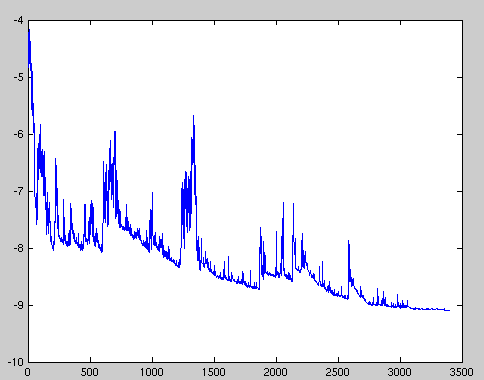
\includegraphics[width=\textwidth]{images/sgd.png}
      \caption{An illustration of \ac{SGD} fluctuations during training as taken from \cite{ref:sgd:2006}.}
      \label{fig:heuristics:gd:sgd}
\end{figure}

With batch learning, all the training patterns are presented at once and the \ac{FFNN} converges to the minimum of the loss/cost function w.r.t $w$. However, this is computationally expensive and intractable to implement in many situations. While \ac{SGD} is able to jump out of local minima into new, potentially better local minima \cite{ref:ruder:2016}, it does at first this seems advantageous. However, this complicates convergence to the exact minima as \ac{SGD} can potentially keep overshooting better minima. It is shown that a slow decrease in the learning rate $\eta$ will lead to the same convergence behaviour as with batch learning, almost certainly converging to local or global minima for non-convex and convex optimisation respectively. A compromise to this problem is to include mini-batches of training patterns where a small number of training patterns are presented to the \ac{FFNN} at once. This means that the input patterns from mini-batches are just approximations of the total population of training patterns. According to \citeauthor{ref:ruder:2016} \cite{ref:ruder:2016} this has two main advantages

\begin{itemize}
      \item Reduces the high variance of weight updates which leads to better convergence
      \item Allows for the implementation of \ac{SGD} using highly optimised matrix operations, common to the state-of-the-art \ac{ML} libraries used today.
\end{itemize}

In the context of this dissertation, \ac{SGD} refers to the mini-batch learning implementation. Although mini-batch \ac{SGD} does provide a compromise between single-pattern and batch learning there are still a number of challenges posed by this approach. These include:

\begin{itemize}
      \item The appropriate value to use for the learning rate $\eta$ is difficult to determine and is often problem-specific. A learning rate that is too small causes premature exploitation, leading to slow and bad convergence. On the contrary, a learning rate that is too high may lead to bad learning outcomes as the heuristic keeps overshooting good minima.

      \item Learning rate schedules \cite{ref:robbins:1951} can be introduced to dynamically change the learning rate throughout the training process, however, these schedules and their parameters have to be defined a priori and are thus problem specific \cite{ref:darken:1992}.

      \item The learning rate that has been introduced so far is applied to all weight updates. If the training data is sparse and the features have very different frequencies an equal update to all weights is inefficient. Larger weight updates are required for less frequently occurring features. This problem eludes to the credit assignment problem \cite{ref:rumelhart:1986} common to these \ac{GD} variants.

      \item It is difficult to avoid getting trapped in local minima, especially for highly non-convex loss/cost functions used for \ac{ANN} training. \cite{ref:dauphin:2014} argues that this difficulty arises not from local minima, but from sadle points. Sadle points are points at which one dimensions slopes upwards while another dimension slopes downwards. \cite{ref:ruder:2016} mentions that these sadle points are usually surrounded by plateaus of the same error, leading to gradients that are close to zero in all dimensions.
\end{itemize}


Alternative methods have been proposed that lead to better control over the convergence characteristics caused by \ac{GD} variants. The first of these include \ac{Momentum} and is presented next.


\subsection{Momentum}
\label{sec:heuristics:gd:momentum}

Research shows that \ac{SGD} has difficulty navigating ravines i.e. areas where the surface curves much more steeply in one dimension than in another \cite{ref:sutton:1986}. These ravines are common around local minima. As such, \ac{SGD} is shown to oscillate across the slopes of the ravine while only making minor progress towards the local minima. An illustration of this is given in Figure~\ref{fig:heuristics:gd:sgd_with_and_without_momentum}.

\begin{figure}[htbp]
      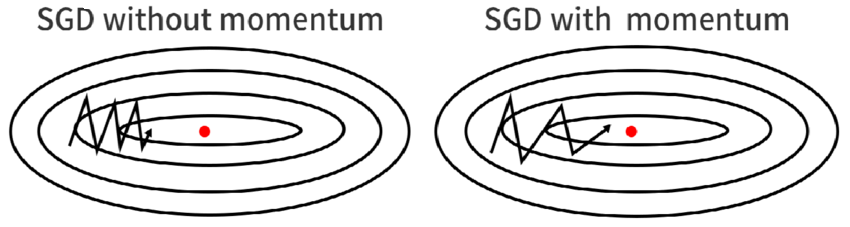
\includegraphics[width=\textwidth]{images/sgd_with_and_without_momentum.png}
      \caption{An illustration of \ac{SGD} with and without momentum taken from \cite{ref:du:2019}.}
      \label{fig:heuristics:gd:sgd_with_and_without_momentum}
\end{figure}

Momentum \cite{ref:qian:1999} is a variant of the \ac{SGD} that helps accelerate \ac{SGD} in the relevant direction, dampening oscillations. \cite{ref:ruder:2016} mentions that this is done by adding a fraction $\alpha$ of the weight update vector of the previous timestep to the current weight update vector. The accumulation of momentum is presented in Equation~\ref{eq:heuristics:gd:momentum_part_1} while the update step is then amended in Equation~\ref{eq:heuristics:gd:momentum_part_2} below.

\begin{equation}
      \label{eq:heuristics:gd:momentum_part_1}
      \begin{split}
            v_{t} = \alpha v_{t-1} + \eta \nabla_{w}\mathcal{E}(w)
      \end{split}
\end{equation}

\begin{equation}
      \label{eq:heuristics:gd:momentum_part_2}
      \begin{split}
            w = w - v_{t}
      \end{split}
\end{equation}

By redefining the \ac{SGD} update steps as shown above, the \ac{Momentum} heuristic allows for the increase of momentum for dimensions whose gradients point in the same direction, while simultaneously reducing momentum for dimensions whose gradients change direction, leading to faster convergence and less oscillation. The momentum term $\alpha$ is usually set to 0.9 \cite{ref:engelbrecht:2007}\cite{ref:ruder:2016}.


\subsection{Nesterov Accelerated Gradients}
\label{sec:heuristics:nag}

\Acl{NAG} is a variant of the \ac{Momentum} heuristics developed by Ilya Sutskever \cite{ref:sutskever:2013-2} and is inspired from Yurii Nesterov's \cite{ref:nesterov:1983} work on optimising convex functions. \ac{NAG} provides an improvement to the momentum accumulation term by providing a look-ahead term that better refines the weight update step. In the \ac{NAG} heuristic, the gradient is not calculated w.r.t the current weights, but rather w.r.t the approximate future positions of the weights \cite{ref:ruder:2016}. An illustration of this is taken from Geoffrey Hinton's lecture on mini-batch \ac{GD} \cite{ref:hinton:2012} and is presented in Figure~\ref{fig:heuristics:gd:nag} below.

\begin{figure}[htbp]
      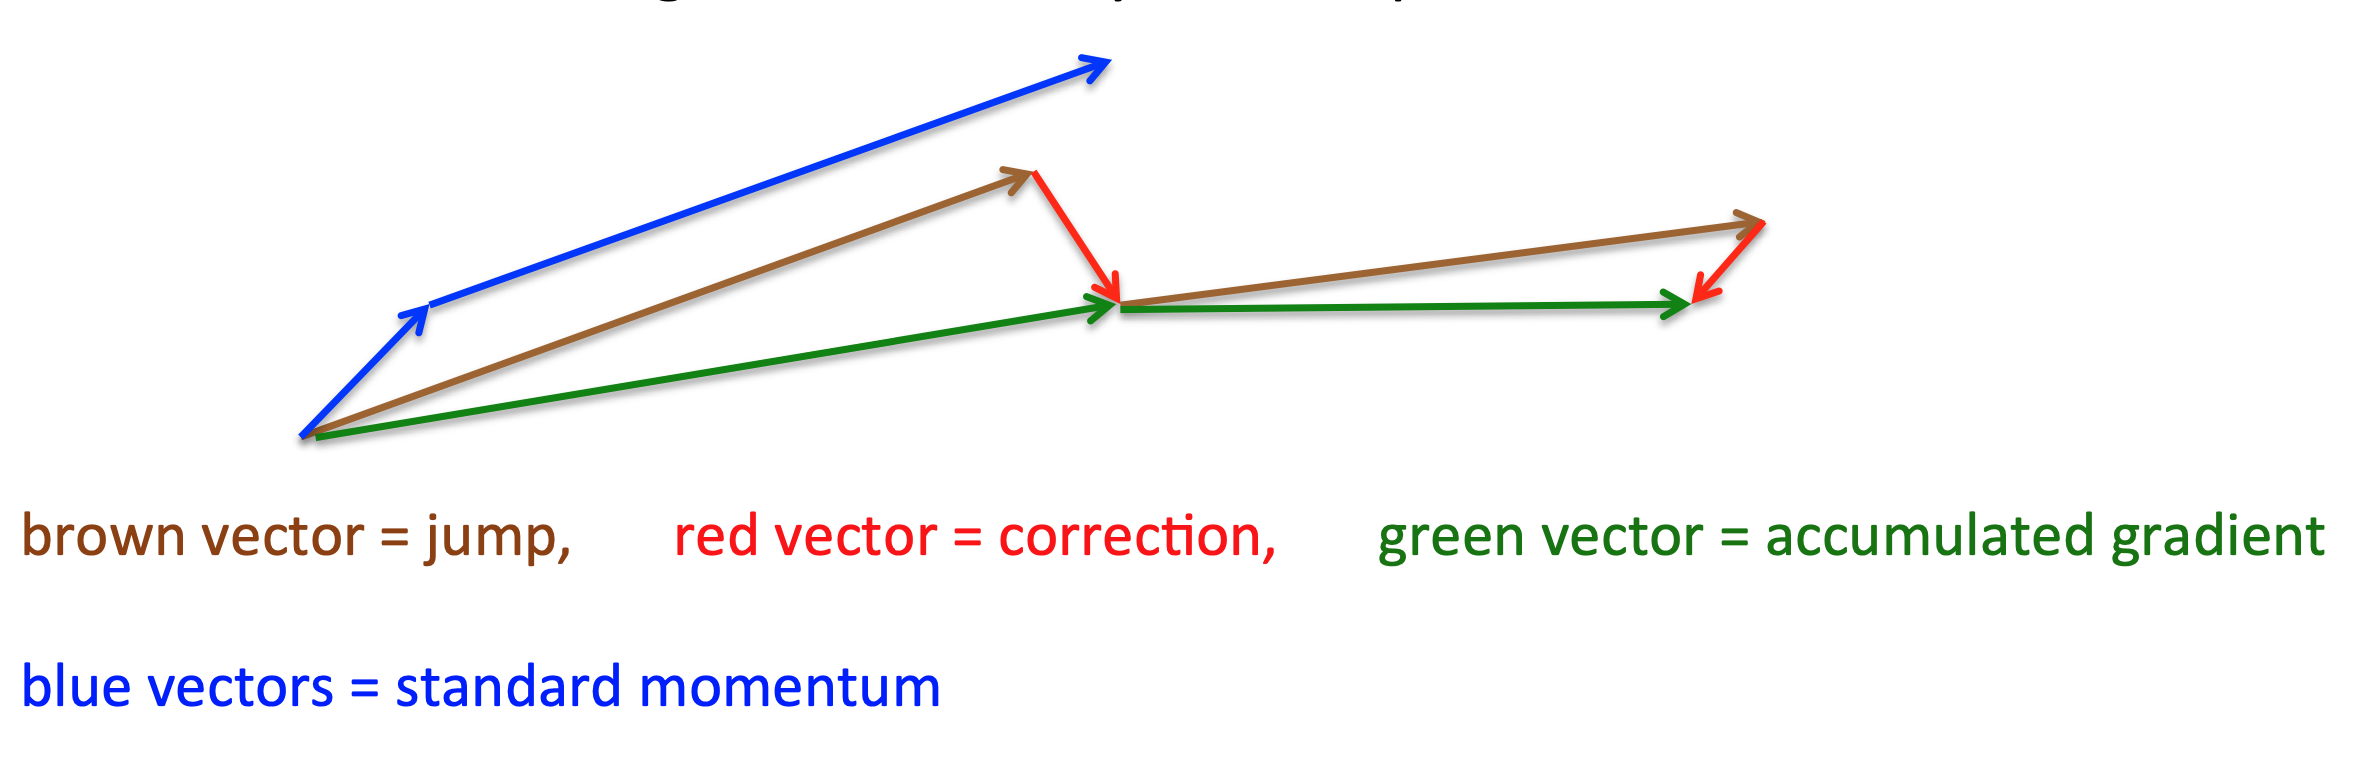
\includegraphics[width=\textwidth]{images/nag.png}
      \caption{An illustration of the weight update vector for \ac{NAG} taken from \cite{ref:hinton:2012}.}
      \label{fig:heuristics:gd:nag}
\end{figure}


\citeauthor{ref:ruder:2016} \cite{ref:ruder:2016} explains the update step as is done by \ac{NAG} is follows. \ac{Momentum} first computes the current gradient. This is seen by the small blue vector presented in Figure~\ref{fig:heuristics:gd:nag}. A large step is taken in the direction of the updated accumulated gradient, presented by the big blue vector. \ac{NAG} then first takes a big step in the direction of the previous accumulated gradient presented by the brown vector. At this point the gradient is measured and \ac{NAG} then makes a correction (red vector), which results in the complete NAG update (green vector). By anticipating approximate future positions of the weights, the weight update step as defined by \ac{NAG} controls the optimisation process from from going too fast and results in increased responsiveness. The \ac{NAG} weight vector update steps are given in Equations~\ref{eq:heuristics:gd:nag_part_1} and~\ref{eq:heuristics:gd:nag_part_2} below.

\begin{equation}
      \label{eq:heuristics:gd:nag_part_1}
      \begin{split}
            v_{t} = \alpha v_{t-1} + \eta \nabla_{w}\mathcal{E}(w - \alpha v_{t-1})
      \end{split}
\end{equation}

\begin{equation}
      \label{eq:heuristics:gd:nag_part_2}
      \begin{split}
            w = w - v_{t}
      \end{split}
\end{equation}

The next logical step in the improvement of the weight vector update step is to tailor the update steps for each weight parameter controlling the magnitude of the update step based on the relevance and importance for that dimension.

\subsection{Adaptive Gradients}
\label{sec:heuristics:adagrad}

\Acl{Adagrad} is an adaptation of \ac{SGD} which implements a learning rate for every parameter in the weight vector and is developed by Duchi et al. \cite{ref:duchi:2011}. \citeauthor{ref:ruder:2016} \cite{ref:ruder:2016} mentions that \Ac{Adagrad} adapts the learning rate to the weights, performing small updates (i.e. low learning rates) for weights associated with frequently occurring features and larger updates (i.e. high learning rates) for weights associated with infrequent features. For this reason \ac{Adagrad} is well suited for dealing with situations with very sparse training data.

In the \ac{GD} variants presented thus far, the weight updates have been applied to all weights at once using the same learning rate $\eta$ for all dimensions of the weight update vector. \Ac{Adagrad} uses a different learning rate for every weight $w_{i}$ at every timestep $t$. The weight update step as implemented by \ac{Adagrad} is presented in Equation~\ref{eq:heuristics:gd:adagrad_part_1} below.

\begin{equation}
      \label{eq:heuristics:gd:adagrad_part_1}
      \begin{split}
            w_{t+1,i} = w_{t,i} - \frac{\eta}{\sqrt{G_{t,ii} + \epsilon}}.\nabla_{w_{i}}\mathcal{E}(w_{t,i})
      \end{split}
\end{equation}

where $w_{i}$ is the $i$-th dimension of the weight vector, $G_{ii} \in \mathbb{R}^{d \times d}$ is a diagonal matrix where each diagonal element $i,i$ is the sum of the squared of the gradients w.r.t. $w_{i}$ up to timestep $t$ and $\epsilon$ is a smoothing term that avoids division by zero, usually set in the order of $1 \times 10^{-8}$ \cite{ref:ruder:2016}. Since $G_{t}$ contains the sum of the squares of the gradients with respect to all parameters $w$ along its diagonal, the weight update step can be vectorised and updated using the matrix-vector product between $G_{t}$ and $\nabla_{w_{i}}\mathcal{E}(w_{i})$. This is presented in Equation~\ref{eq:heuristics:gd:adagrad_part_2} below.

\begin{equation}
      \label{eq:heuristics:gd:adagrad_part_2}
      \begin{split}
            w_{t+1} = w_{t} - \frac{\eta}{\sqrt{G_{t} + \epsilon}} \odot \nabla_{w_{i}}\mathcal{E}(w_{t})
      \end{split}
\end{equation}

\Ac{Adagrad}'s main benefit is that it does not require the need to manually tune the learning rate. However, a problem with \ac{Adagrad} is the accumulation of the sums of squared gradients in the denominator. Since every term that is added is positive, this number keeps growing, leading to a situation where the learning rate shrinks to the point that the heuristic is no longer able to learn. \acl{Adadelta} aims to improve on this problem.

\subsection{Adaptive Learning Rate}
\label{sec:heuristics:adadelta}

In Section~\ref{sec:heuristics:adagrad} it was mentioned that one of the main problems of \ac{Adagrad} is that it has an aggressively monotonically decreasing learning rate because of the accumulation of the sum of squared gradients in its denominator. Zeiler \cite{ref:zeiler:2012} presents an improvement on \ac{Adagrad} that eliminates this problem. \citeauthor{ref:ruder:2016} \cite{ref:ruder:2016} mentions that instead of accumulating all past squared gradients as in the case of \ac{Adagrad}, \ac{Adadelta} restricts the window of accumulation to a window with a fixed size $W$. However, storing $W$ previous squared gradients is very inefficient. Instead, the accumulation of the sum of gradients over $W$ steps is defined recursively as a decaying average of all past squared gradients. The moving average $E[g^{2}]_{t}$ at timestep $t$ then depends only a fraction $\alpha$ of the previous average and current gradient, similar to the update step for \ac{Momentum}. In order to simplify the notation of update steps, let $g = \nabla_{w_{i}}\mathcal{E}(w_{t})$. The moving average update step for $E[g^{2}]_{t}$ is then presented in Equation~\ref{eq:heuristics:gd:adadelta_part_1} below.

\begin{equation}
      \label{eq:heuristics:gd:adadelta_part_1}
      \begin{split}
            E[g^{2}]_{t} = \alpha E[g^{2}]_{t - 1} + (1 - \alpha)g_{t}^{2}
      \end{split}
\end{equation}

The value for $\alpha$ is set to a similar value, 0.9, as was done with \ac{Momentum}. For sake of clarity, the basic \ac{SGD} update step is rewritten in terms of the weight update vector $\Delta w_{t}$. This is presented in Equations~\ref{eq:heuristics:gd:adadelta_part_2} and~\ref{eq:heuristics:gd:adadelta_part_2} below.

\begin{equation}
      \label{eq:heuristics:gd:adadelta_part_2}
      \begin{split}
            \Delta w_{t} = -\eta g_{t,i}
      \end{split}
\end{equation}

\begin{equation}
      \label{eq:heuristics:gd:adadelta_part_3}
      \begin{split}
            w_{t+1} = w_{t} + \Delta w_{t}
      \end{split}
\end{equation}

The weight update vector for \ac{Adagrad} as defined in Equation~\ref{eq:heuristics:gd:adagrad_part_2} is then rewritten as


\begin{equation}
      \label{eq:heuristics:gd:adagrad_part_2_new}
      \begin{split}
            \Delta w_{t} = - \frac{\eta}{\sqrt{G_{t} + \epsilon}} \odot g_{t}
      \end{split}
\end{equation}

The diagonal matrix $G_{t}$ is then replaced with the decaying average over the past $W$ squared gradients as presented in Equation~\ref{eq:heuristics:gd:adadelta_part_4} below.

\begin{equation}
      \label{eq:heuristics:gd:adadelta_part_4}
      \begin{split}
            \Delta w_{t} = - \frac{\eta}{\sqrt{E[g^{2}]_{t} + \epsilon}} g_{t}
      \end{split}
\end{equation}

Since the denominator is the \ac{RMS} error criterion of the gradient, the criteria short-hand notation is used as follows.

\begin{equation}
      \label{eq:heuristics:gd:adadelta_part_5}
      \begin{split}
            \Delta w_{t} = - \frac{\eta}{RMS[g]_{t}} g_{t}
      \end{split}
\end{equation}

\citeauthor{ref:ruder:2016}\cite{ref:ruder:2016} highlights that the original authors \cite{ref:zeiler:2012} noted that the units of the update step as presented in Equation~\ref{eq:heuristics:gd:adadelta_part_2} do not match i.e. the update vector should have the same hypothetical units as the weight vector. To realize this, another exponentially decaying average is defined in terms of squared weight updates as is presented in Equation~\ref{eq:heuristics:gd:adadelta_part_6} below.

\begin{equation}
      \label{eq:heuristics:gd:adadelta_part_6}
      \begin{split}
            E[\Delta w^{2}]_{t} = \alpha E[\Delta w^{2}]_{t - 1} + (1 - \alpha)\Delta w^{2}
      \end{split}
\end{equation}

The \ac{RMS} error of weight updates is thus

\begin{equation}
      \label{eq:heuristics:gd:adadelta_part_7}
      \begin{split}
            RMS[\Delta w]_{t} = \sqrt{E[\Delta w^{2}]_{t} + \epsilon}
      \end{split}
\end{equation}

Note that $RMS[\Delta w]_{t}$ is unknown at timestep $t$. It is thus approximated with the \ac{RMS} of weight updates until the previous timestep. The learning rate in Equation~\ref{eq:heuristics:gd:adadelta_part_5} is then replaced as follows.

\begin{equation}
      \label{eq:heuristics:gd:adadelta_part_8}
      \begin{split}
            \Delta w_{t} = - \frac{RMS[\Delta w]_{t-1}}{RMS[g]_{t}} g_{t}
      \end{split}
\end{equation}

Finally, the weight update step for \ac{Adadelta} is concluded as follows.

\begin{equation}
      \label{eq:heuristics:gd:adadelta_part_9}
      \begin{split}
            w_{t+1} = w_{t} + \Delta w_{t}
      \end{split}
\end{equation}

The main advantage of \ac{Adadelta} is that one does not have to provide a default learning rate a priori as it is no longer included in the weight update step.

\subsection{Root Mean Squared Error Propagation}
\label{sec:heuristics:rmsprop}

\Ac{RMSProp} is a similar heuristic to \ac{Adadelta} presented by Geoffrey Hinton \cite{ref:hinton:2012} and was developed independently around the same time. \citeauthor{ref:ruder:2016}\cite{ref:ruder:2016} mentions that \ac{RMSProp} is in fact the same as the first weight update vector as defined for \ac{Adadelta}. The update step for \ac{RMSProp} is then defined in terms of a decaying running average of gradients squared as is presented again for convenience in Equations~\ref{eq:heuristics:gd:rmsprop_part_1} and~\ref{eq:heuristics:gd:rmsprop_part_2} below.


\begin{equation}
      \label{eq:heuristics:gd:rmsprop_part_1}
      \begin{split}
            E[g^{2}]_{t} = \alpha E[g^{2}]_{t - 1} + (1 - \alpha)g_{t}^{2}
      \end{split}
\end{equation}

\begin{equation}
      \label{eq:heuristics:gd:rmsprop_part_2}
      \begin{split}
            w_{t+1} = w_{t} - \frac{\eta}{\sqrt{E[g^{2}]_{t} + \epsilon}} g_{t}
      \end{split}
\end{equation}

Note that \ac{RMSProp} still includes the learning rate term $\eta$ meaning that a default learning rate is required a priori. This is one of the disadvantages of \ac{RMSProp}. Hinton suggests $\alpha$ be set to 0.9 and $\eta$ be set to $0.001$ \cite{ref:hinton:2012}.


\subsection{Adaptive Moments Estimation}
\label{sec:heuristics:adam}

\Ac{Adam} is another variant of \ac{SGD} that includes adaptive learning rates and is presented by Kingma et. al \cite{ref:kingma:2014}. However, in addition to storing an exponentially decaying average of past squared gradients like \ac{Adadelta} and \ac{RMSProp}, \ac{Adam} also stores an exponentially decaying average of past gradients $v_{t}$, similar to \ac{Momentum} \cite{ref:ruder:2016}. \citeauthor{ref:heusel:2017} \cite{ref:heusel:2017} uses the analogy that \ac{Momentum} can be seen as a ball running down a slope, while \ac{Adam} behaves like a heavy ball with friction, which thus prefers flat minima in the error surface.

The decaying averages for past gradients and past squared gradients is given in Equations~\ref{eq:heuristics:gd:adam_part_1} and~\ref{eq:heuristics:gd:adam_part_2} respectively.

\begin{equation}
      \label{eq:heuristics:gd:adam_part_1}
      \begin{split}
            m_{t+1} = \beta_{1}m_{t} + (1 - \beta_{1})g_{t}
      \end{split}
\end{equation}


\begin{equation}
      \label{eq:heuristics:gd:adam_part_2}
      \begin{split}
            v_{t+1} = \beta_{2}v_{t} + (1 - \beta_{2})g^{2}_{t}
      \end{split}
\end{equation}

In Equations~\ref{eq:heuristics:gd:adam_part_1} and~\ref{eq:heuristics:gd:adam_part_2} above, $\beta_{1}$ and $\beta_{2}$ are decay rates, similar to $\alpha$ for \ac{Momentum}.

\citeauthor{ref:ruder:2016} \cite{ref:ruder:2016} mentions that $v_{t}$ and $w_{t}$ presented above are estimates of the first moment (the mean) and the second moment (the uncentered variance) of the gradients respectively. It is from these moment terms that the name \acl{Adam} is derived. \citeauthor{ref:kingma:2014} \cite{ref:kingma:2014} mentions that because $v_{t}$ and $w_{t}$ is initialised to be vectors of 0's, they are biased towards 0. This is especially true during the initial timesteps and/or when the decay rates $\beta_{1}$ and $\beta_{2}$ are small (i.e. $\beta_{1}$ and $\beta_{2}$ is close to 1). These biases need to be corrected. The bias-corrected first and second moment estimates are presented in Equations~\ref{eq:heuristics:gd:adam_bc_first_moment} and~\ref{eq:heuristics:gd:adam_bc_second_moment} below.

\begin{equation}
      \label{eq:heuristics:gd:adam_bc_first_moment}
      \begin{split}
            \hat{m}_{t} = \frac{m_{t}}{1 - \beta^{t}_{1}}
      \end{split}
\end{equation}


\begin{equation}
      \label{eq:heuristics:gd:adam_bc_second_moment}
      \begin{split}
            \hat{v}_{t} = \frac{v_{t}}{1 - \beta^{t}_{2}}
      \end{split}
\end{equation}

The \ac{Adam} update rule is then presented in Equation~\ref{eq:heuristics:gd:adam} below.

\begin{equation}
      \label{eq:heuristics:gd:adam}
      \begin{split}
            w_{t+1} = w_{t} - \frac{\eta}{\sqrt{\hat{v}_{t}} + \epsilon}\hat{m}_{t}
      \end{split}
\end{equation}

\citeauthor{ref:kingma:2014} \cite{ref:kingma:2014} suggest default values $B_{1}=0.9$, $B_{2}=0.999$ and $\epsilon = 1 \times 10^{-8}$. This section provided the reader with a collection of gradient-based heuristics. The next section introduces meta-heuristics.

\section{Meta-Heuristics}
\label{sec:heuristics:mh}

Gradient-based methods are sensitive to the type of problem that they it applied to, with hyper-parameter selection often dominating the research focus \cite{ref:bengio:2000}\cite{ref:feurer:2019}. In the context of \acp{HH}, it is important to consider a diverse set of low-level heuristics to select from. Apart from gradient-based methods, alternative heuristics must thus be considered. \cite{ref:blum:2003} mentions since the 1980's, a new kind of approximate algorithm has emerged which basically tries to combine basic heuristic methods in higher level frameworks aimed at efficiently and effectively exploring a search space. These methods referred to as metaheuristics. This section aims to introduce the reader to the concept of meta-heuristics. Specifically, this section focuses on population-based meta-heuristics. Three well known meta-heuristics are presented. Each of these have been shown to train \ac{FFNN}. These meta-heuristics include \ac{PSO}, \ac{DE} and \acp{GA}. \cite{ref:carvalho:2006} compared various \ac{PSO} variants for training \acp{FFNN}. \cite{ref:espinal:2011} compared \ac{DE} and \ac{PSO} when applied to \ac{FFNN} training and \cite{ref:gupta:1999} compared \ac{BP} to a \ac{GA} for training \acp{FFNN}.

A formal definition for meta-heuristics is required. The term \aclp{MH} was first introduced by \citeauthor{ref:glover:1986}\cite{ref:glover:1986} in 1986. The world derives from the composition of two Greek words. Heuristic derives from the verb \textit{heuriskein} which means ``to find''. The suffix, \textit{meta} means ``beyond, in an upper level''. Before this term was widely adopted, \acp{MH} were often called \textit{modern heuristics} \cite{ref:reeves:1993}. \cite{ref:blum:2003} mentions that there is a debate as to what the formal defintion of \acp{MH} is and suggests the definition of \acp{MH} to be high level strategies for exploring search spaces by using different methods. \citeauthor{ref:blum:2003} \cite{ref:blum:2003} provides characterists of meta-heuristics. These characterists are given as follows.

\begin{itemize}
      \item \ac{MH} are strategies to guide the search process.

      \item The goal of \acp{MH} is to efficiently explore the search space in order to find (near) optimal solutions.

      \item Techniques that constitute \ac{MH} algorithms range from simple local search to complex learning processes.

      \item \ac{MH} algorithms are approximate and usually non-deterministic.

      \item \acp{MH} may incorporate some mechanism to avoid getting trapped in local minima.

      \item The basic concept of \acp{MH} permit an abstract level description.

      \item \acp{MH} are not problem-specific.

      \item \acp{MH} may make use of domain-specific knowledge  in the form of heuristics that are controlled by the upper level strategy.

      \item Today's more advanced \acp{MH} use search experience (embodied in some form of memory) to guide the search/optimisation process.
\end{itemize}

\citeauthor{ref:blum:2003} \cite{ref:blum:2003} proposes the classification of heuristics as follows:

\begin{itemize}
      \item Nature inspired vs. non-nature inspired.
      \item Population-based vs. single point search.
      \item Dynamic vs. statis objective functions.
      \item One vs. various neighbourhood structures.
      \item Memory usage vs. memory-less methods.
\end{itemize}

The first of these \ac{MH} algorithms that are relevant to this dissertation include \ac{PSO}. The concept of \acp{PSO} is presented and discussed next.


\subsection{Particle Swarm Optimisation}
\label{sec:heuristics:mh:pso}

\Ac{PSO} is a stochastic population-based search algorithm based on the social behaviour of birds in a flock \cite{ref:kennedy:1995}. By definition, the \ac{PSO} heuristic is nature-inspired.  \Acp{PSO} were first presented  by \citeauthor{ref:kennedy:1995}\cite{ref:kennedy:1995}. It was also Kennedy and Eberhart that first applied \acp{PSO} to train of \acp{FFNN} \cite{ref:eberhart:1995}\cite{ref:kennedy:1997}. The application of \acp{PSO} in the context of training \ac{FFNN} have been widely studied \cite{ref:rakitianskaia:2012}\cite{ref:vanwyk:2014} and it has been found to perform well. This section aims to provide the reader with the detail of \ac{PSO} implementation.

In general, this dissertation uses the term \textit{entity} for candidate solutions and a \textit{population} for a collection of entities. \citeauthor{ref:engelbrecht:2007}\cite{ref:engelbrecht:2007} mentions that in \acp{PSO} individual candidate solutions are referred to as \textit{particles} and the population is referred to as a \textit{swarm}. These particles are ``flown'' through a hyperdimensional space. Changes in particle position is due to social-psychological tendencies of individuals to emulate the success of other individuals. The changes in the particle position are then influenced by the experience or knowledge of the particle's neighbours. It can be said that the position of a particle is thus influenced by the positions of other particles in the swarm resulting in a symbiotic cooperative heuristic. The social behaviour of particles is modeled such that they stochastically return to previously successful regions in the search space.

\citeauthor{ref:vanwyk:2014}\cite{ref:vanwyk:2014} mentions that the swarm is usually arranged in a predefined structure, called a \textit{neighbourhood topology} that governs the communication between particles. Two different configurations of neighbourhood topologies exists. These are referred to as \textit{Local best (lbest)} \ac{PSO} and \textit{global best (gbest)} \ac{PSO}. There are two main differences between the two approaches in terms of their convergence characteristics \cite{ref:eberhart:1996}. These include:

\begin{itemize}
      \item Due to the larger particle interconnectivity of \textit{gbest} \ac{PSO}, the heuristic converges faster than with \textit{lbest} \ac{PSO}. \cite{ref:engelbrecht:2007} mentions that faster convergence comes at a cost of less diversity.
      \item As a consequence of larger diversity, the \textit{lbest} \ac{PSO} is less susceptible to getting trapped in local minima.
\end{itemize}

\citeauthor{ref:shi:1998}\cite{ref:shi:1998} proposed a modification of the original \ac{PSO} as was presented by \citeauthor{ref:kennedy:1995}. Their implementation focuses on the \textit{gbest} \ac{PSO} with \textit{inertia} weights. This dissertation focuses on their implementation of \textit{global best} \ac{PSO} and is discussed next.

The particles in this configuration has a number of properties associated with them \cite{ref:vanwyk:2014}. These include:

\begin{itemize}
      \item \textbf{Position}: Refers to the candidate solution that is represented by the particle and defines the particle position within the optimisation problem's hyper-dimensional solution space. Let the current position of particle $i$ at timestep $t$ be denoted by $x_{i}(t)$ and let $N$ be the search space dimensionality.
      \item \textbf{Velocity}: Represents a step size for the particle in the search space. The velocity vector of particle $i$ at timestep $t$ is denoted $v_{i}(t)$.
      \item \textbf{Solution Quality}: Refers to the evaluation of the particle's position with respect to the objective function. Let $f(x_{i}(t)$ denote the quality of the solution represented by the particle's position.
      \item \textbf{Personal Best Position}: Refers to a cognitive memory construct where each particle keeps track of their personal best position found during optimisation thus far. The personal best position is denoted $y_{i}(t)$.
      \item \textbf{Global Best Position}: Refers to a social memory construct where the each particle has a reference to the best solution found in the particle's neighbourhood thus far. In the case of \text{gbest} \ac{PSO}, the global best position is the best position of the entire swarm. The personal best position is denoted $\hat{y}_{i}(t)$.
\end{itemize}

During initialisation particles are randomly places within the search space by sampling from a uniform distribution such that $x_{i} \sim U(x_{min}, x_{max})$ and the velocity is set to vector of 0 such that $v_{i} = 0$. At timestep 0, the particle's initial position is set to be the particle's personal best solution such that $y_{i}(0) = x_{i}(0)$. The particle's update step is then broken into two parts. These include a velocity update step presented in Equation~\ref{eq:heuristics:pso:velocity} followed by a position update step as presented in Equation~\ref{eq:heuristics:pso:position} below.

\begin{equation}
      \label{eq:heuristics:pso:velocity}
      \begin{split}
            v_{ij}(t+1) = wv_{ij}(t) + c_{1}r_{1}(t)[y_{ij}(t) - x_{ij}(t)] + c_{2}r_{2}(t)[\hat{y}_{ij}(t) - x_{ij}(t)]
      \end{split}
\end{equation}

\begin{equation}
      \label{eq:heuristics:pso:position}
      \begin{split}
            x_{ij}(t+1) = x_{ij}(t) + v_{ij}(t+1)
      \end{split}
\end{equation}

In Equations~\ref{eq:heuristics:pso:velocity} and~\ref{eq:heuristics:pso:position}, $i$ refers to the $i$-th particle in the swarm, $j$ refers to the $j$-th dimension of vectors with dimensionality $N$ defined by the optimisation problem. A breakdown of the components introduced above is required. The velocity update step consists of:

\begin{itemize}
      \item \textbf{Previous Velocity}: Denoted by the term $wv_{ij}(t)$. This term represents the particle's momentum and is used to formulate an update step for the particle in the search space. \citeauthor{ref:vanwyk:2014}\cite{ref:vanwyk:2014} mentions that it forces the particle to maintain a consistent direction, preventing drastic changes in terms of update steps. This term is then scaled by the \textit{inertia} weight control parameter, denoted $w$. Inertia weight was introduced by \citeauthor{ref:shi:1998}\cite{ref:shi:1998} as a mechanism to control the exploration and exploitation abilities of the swarm. It was also introduced as a mechanism to eliminate velocity clamping (discussed later in the section). The introduction of inertia weight was successful in addressing the first objective, however did not quite provide a way to totally eliminate velocity clamping \cite{ref:shi:2001}.

      \item \textbf{Cognitive Component}: Denoted by the term $c_{1}r_{1}(t)[y_{ij} - x_{ij}(t)]$. This component represents the particle's personal  experience. It introduces an attractor to the particle's personal best position so far. The cognitive component is stochastically scaled with random numbers $r{1} \sim U(0,1)^N$ and the cognitive acceleration coefficient $c_{1}$ is used to control the influence of the cognitive attractor.

      \item \textbf{Social Component}: Denoted by the term $c_{2}r_{2}(t)[\hat{y}_{ij} - x_{ij}(t)]$. This component represents the particle's social  experience. It introduces an attractor to the swarm's best position so far. The social component is also stochastically scaled with random numbers $r{2} \sim U(0,1)^N$, while also introducing the social acceleration coefficient $c_{2}$ that is used to control the influence of the social attractor.
\end{itemize}

A concept known as \textit{velocity clamping} is mentioned above. \citeauthor{ref:vanwyk:2014}\cite{ref:vanwyk:2014} mentions that when \acp{PSO} where first developed, it was possible for particle velocities to become inappropriately large during optimisation leading to situations where particles fly out of the feasible search space. This is known as \textit{swarm explosion} and occurs when there are frequent changes in the global best position. In order to address this issues, the concept of \textit{velocity clamping} was introduced \cite{ref:eberhart:1996}. The idea behind velocity clamping is to restrict particle velocities to some $V_{max}$ threshold, in essence, modeling a form of terminal velocity. Velocity clamping is applied after the velocity update step and is given in Equation~\ref{eq:heuristics:pso:velocity_clamping} below.

\begin{equation}
      \label{eq:heuristics:pso:velocity_clamping}
      \begin{split}
            v_{ij}(t+1)=
            \begin{cases}
                  v'_{ij}(t+1) & \text{if } |v'_{ij}(t+1)| < V_{max,j}   \\
                  -V_{maxj}    & \text{if } v'_{ij}(t+1) \leq -V_{max,j} \\
                  V_{maxj}     & \text{if } v'_{ij}(t+1) \geq V_{max,j}
            \end{cases}
      \end{split}
\end{equation}

$V_{max}$ then becomes another hyper-parameter that must be defined a priori. Appropriate values $V_{max}$ may prevent swarm explosion, but also has an effect on the exploration and exploitation of the heuristic. If $V_{max}$ is small, particle update steps are small, resulting in exploitation \cite{ref:eberhart:1996}. If $V_{max}$ is big, it allows for larger update steps, promoting more exploration. A balance is needed between exploration and exploitation. Similar to other strategies, such as learning rate schedules for gradient-based heuristics, adaptive strategies such as those proposed in \cite{ref:fan:2002} have been developed, but are beyond the scope of this dissertation.

It should be noted that the choice of control parameter play a vital role on the behaviour and characteristics of the \ac{PSO}. Van den Berg and Engelbrecht \cite{ref:vandenberg:2007}\cite{ref:vandenberg:2006} have done extensive work on the effects of different values for control parameters. For the purposes of this dissertation, the $c_{1}$ and $c_{2}$ control parameter are set to $1.496180$ and the inertia weight $w$ is set to $0.0729844$ as these correspond to values used in \cite{ref:eberhart:2000} and have been shown to be appropriate for a number of problems.

An example of the pseudo code implementation of the \textit{gbest} \ac{PSO} is taken from \cite{ref:engelbrecht:2007} and is given in Algorithm~\ref{algo:heuristics:pso:gbest} below.

\begin{algorithm}[H]
      \caption{The pseudo code algorithm for the gbest \ac{PSO} heuristic.}
      \label{algo:heuristics:pso:gbest}
      \begin{algorithmic}
            \State Create and initialise an $N_{x}$ dimensional swarm;
            \While{stopping condition not met}
            \For{each particle $i = 1, \dots, N_{s}$}
            \State // Set the personal best position;
            \If{$f(x_{i}) < f(y_{i})$ }
            \State $y_{i} = x_{i}$;
            \EndIf

            \State // Set the global best position;
            \If{$f(x_{i}) < f(\hat{y})$ }
            \State $\hat{y} = x_{i}$;
            \EndIf
            \EndFor

            \For{each particle $i = 1, \dots, N_{s}$}
            \State // Perform velocity update step;
            \State $v_{ij} = wv_{ij} + c_{1}r_{1}[y_{ij} - x_{ij}] + c_{2}r_{2}[\hat{y}_{ij} - x_{ij}]$
            \State // Perform position update step;
            \State $x_{ij} = x_{ij} + v_{ij}$
            \EndFor
            \EndWhile
      \end{algorithmic}
\end{algorithm}

This section provided the reader with the implementation details of the \ac{PSO} heuristic. It was mentioned that \ac{PSO} have been used to train \acp{FFNN} on many occasions with successful outcomes. The following section presents the reader with the next population-based \ac{MH} that is considered.

\subsection{Differential Evolution}
\label{sec:heuristics:mh:de}

This section aims to introduce the reader to the next population-based \ac{MH} called \acl{DE}. Similar to \ac{PSO}, \Ac{DE} is a stochastic population-based search strategy developed by Storm and Price \cite{ref:price:2006} in 1995. \Ac{DE} shares a lot of similarities with other evolutionary \ac{MH} paradigms such as \acp{PSO} and \acp{GA}. However, \ac{DE} differs significantly in the sense that it makes use of distance and direction information from the current population to guide the search process \cite{ref:engelbrecht:2007}. Originally, \ac{DE} was focused on multi-dimensional real-values optimisation problems, but unlike gradient-based heuristics, it does not require any gradient information. This means that \ac{DE} does not require the underlying optimisation problem to be differentiable, meaning that it can be applied to problems that are discrete, noisy and dynamic \cite{ref:rocca:2011}.

Lots of research has been done on using \ac{DE} to train \acp{FFNN}. Some notable work include \cite{ref:ilonen:2003}\cite{ref:slowik:2008}\cite{ref:mingguang:2009}. In these works, the authors often highlight the low computational complexity and simplicity of implementation for \ac{DE}.

Similar to other \acp{EA}, variation from one generation to the next is achieved through the application of crossover and mutation operators. Engelbrecht \cite{ref:engelbrecht:2007} mentions that for other \acp{EA} if both these operators are used, crossover is applied first after which the generated offspring is mutated. For other \acp{EA} mutation step sizes are sampled from some probability distribution. \ac{DE} differs from these implementations in that

\begin{itemize}
      \item mutation is applied first to generate a \textit{trial vector}, which is then used within the crossover operator to produce one offspring and
      \item mutation step sizes are not sampled from prior known probability distributions.
\end{itemize}

In \ac{DE} mutation step sizes are influenced by the differences in positions of different entities in the current population. The positions of entities in the population provide valuable information about the fitness landscape. This is under the assumption that entities are initially uniformly placed in the search space. \ac{DE} aims to exploit this concept in order to find optimal solutions. There are three main components to the \ac{DE} heuristic. These include mutation, crossover and selection operators \cite{ref:price:2006}. Each of these are presented briefly next.

\subsubsection{Mutation}
\label{sec:heuristics:mh:de:mutation}

The purpose of the mutation operator is to produce a trial vector for each entity in the current population by mutating a target vector with a weighted differential \cite{ref:engelbrecht:2007}. This trial vector is used in the crossover operator (discussed next) to produce offspring. The mutation process then follows as such. For each each parent $x_{i}(t)$ generate a trial vector $u_{i}(t)$ as follows.

\begin{itemize}
      \item Select a target vector, $x_{i_{1}}(t)$ from the population the is not the same as the parent i.e. $i \neq i_{1}$.
      \item This is followed by randomly selecting two other individuals $x_{i_{2}}(t)$ and $x_{i_{3}}(t)$. Importantly, all of these entities must be unique such that $i \neq i_{1} \neq i_{2} \neq i_{3}$ and $i_{2}, i_{3} \sim U(1, N_{s}$ where $N_{s}$ is the size of the swarm.
      \item These individual entities are then used to calculate the trial vector by perturbing the target vector as presented in Equation~\ref{eq:heuristics:de:mutation} below.
\end{itemize}


\begin{equation}
      \label{eq:heuristics:de:mutation}
      \begin{split}
            u_{i}(t) = x_{i_{1}} + \beta(x_{i_{2}}(t) - x_{i_{3}}(t))
      \end{split}
\end{equation}

In Equation~\ref{eq:heuristics:de:mutation} $\beta \in (0, \infty)$ is the scale factor and controls the amplification of the differential variation \cite{ref:engelbrecht:2007}. Note that in the above steps, the selection strategy to select the target vector is not specified. Selection is discussed in Section~\ref{sec:heuristics:mh:de:selection} below.


\subsubsection{Crossover}
\label{sec:heuristics:mh:de:crossover}

In the context of \acp{EA}, reproduction and recombination is done through the crossover operation. The same applies to \ac{DE}. The \ac{DE} crossover operator implements a discrete recombination of the trial vector, $u_{i}(t)$ (as was generated in Section~\ref{sec:heuristics:mh:de:mutation} above) and the parent vector $x_{i}(t)$ to produce new offspring $x'_{i}(t)$. The crossover operator is given in Equation~\ref{eq:heuristics:de:crossover} below.

\begin{equation}
      \label{eq:heuristics:de:crossover}
      \begin{split}
            x'_{ij}(t)=
            \begin{cases}
                  u_{ij}(t) & \text{if } j \in \mathcal{J} \\
                  x_{ij}(t) & \text{otherwise }
            \end{cases}
      \end{split}
\end{equation}

In Equation~\ref{eq:heuristics:de:crossover}, $x_{ij}(t)$ refers to the $j$-th element of the vector $x_{i}(t)$ and $\mathcal{J}$ refers to a set of crossover points or indices at which perturbation is done. Different techniques for determining the set, $\mathcal{J}$ has been proposed \cite{ref:storn:1996}\cite{ref:storn:1997}. These include:

\begin{itemize}
      \item \textbf{Binomial crossover}: A crossover mask is generated by randomly selecting indices from the set of possible crossover points $\{1,2,\dots,N_{x}$ where $N_{x}$ is the problem dimension. This techique is presented in Algorithm~\ref{algo:heuristics:de:bin} below. In Algorithm~\ref{algo:heuristics:de:bin} $p_{r}$ is the crossover probability. The higher the value of $p_{r}$, the more points will be included in the set $\mathcal{J}$. A \textit{Bernoulli} distribution (presented in Chapter~\ref{chap:probability} can be used to generate the binomial crossover mask. Note that due to the probabilistic nature of this process, it is possible that no crossover points are selected. To counteract this situation, a randomly selected crossover point $j^{*}$ is included in the set $\mathcal{J}$ such that $\mathcal{J} \neq \emptyset$ where $\emptyset$ is the empty set.
      \item \textbf{Exponential crossover}: \citeauthor{ref:engelbrecht:2007}\cite{ref:engelbrecht:2007} states that with exponential crossover a sequence of adjacent crossover points are selected start from some randomly selected crossover index. This means that the set of possible crossover points $\mathcal{J}$ is a circular array in indices. This technique does not require the selection of an additional crossover point $j^{*}$ as this technique includes at the very least one index, which is the starting index that is randomly selected. From this point, the next index is selected until $U(0,1) \geq p_{r}$ or $|\mathcal{J}| = N_{x}$. $p_{r}$ is the same crossover probability as mentioned above for binomial crossover. The implementation of exponential crossover is given in Algorithm~\ref{algo:heuristics:de:exp} below.
\end{itemize}

\begin{algorithm}[H]
      \caption{The pseudo code algorithm for the binomial crossover technique for \ac{DE}.}
      \label{algo:heuristics:de:bin}
      \begin{algorithmic}
            \State $j^{*} \sim U(1,N_{x})$;
            \State $\mathcal{J} \gets \mathcal{J} \cup \{j^{*}\}$;
            \For{each $j \in \{1, \dots, N_{x}\}$}
            \If{$U(0,1) < p_{r}$ and $j \neq j^{*}$ }
            \State $\mathcal{J} \gets \mathcal{J} \cup \{j\}$;
            \EndIf
            \EndFor
      \end{algorithmic}
\end{algorithm}

\begin{algorithm}[H]
      \caption{The pseudo code algorithm for the exponential crossover technique for \ac{DE}.}
      \label{algo:heuristics:de:exp}
      \begin{algorithmic}
            \State $\mathcal{J} \gets \{\}$;
            \State $j \sim U(0,N_{x} - 1)$;
            \Repeat
            \State $\mathcal{J} \gets \mathcal{J} \cup \{j + 1 \}$;
            \State $j = (j+1) \mod N_{x}$
            \Until{ $U(0,1) \geq p_{r}$ or $|\mathcal{J} = N_{x}$;}
      \end{algorithmic}
\end{algorithm}

\subsubsection{Selection}
\label{sec:heuristics:mh:de:selection}

Selection refers to the technique that is used to determine which entities are included in the mutation operator to produce a trial vector \cite{ref:engelbrecht:2007} as was shown in Section~\ref{sec:heuristics:mh:de:mutation} above. Various selection operators have been suggested. With reference to the mutation operator, most \ac{DE} implementations make use of random selection or the best entity is used as the target vector $x_{i_{1}}(t)$. To construct the population for the next generation, deterministic selection is used. As such, a parent is replaced if the offspring produces a better solution that the parent such that $f(x'_{i}(t)) \leq f(x_{i}(t))$. \citeauthor{ref:engelbrecht:2007}\cite{ref:engelbrecht:2007} states that this is to ensure the average fitness of the population does not deteriorate.


\subsubsection{General Differential Evolution Algorithm}

Algorithm~\ref{algo:heuristics:de:general_de} is taken from \cite{ref:engelbrecht:2007} and presents the general \ac{DE} algorithm. The population is initialised by randomly placing entities in the search space such that the positions of the entities are confined to some search boundary. As such, $x_{ij}(t) \sim U(x_{min,j}, x_{max,j})$, where $x_{min,j}$ and $x_{max,j}$ define the search boundaries.

\begin{algorithm}[H]
      \caption{The pseudo code for the general \ac{DE} heuristic.}
      \label{algo:heuristics:de:general_de}
      \begin{algorithmic}
            \State Set the generation counter, $t = 0$;
            \State Initialise the control parameters, $\beta$ and $p_{r}$
            \While{stopping condition not met}
            \For{each entity $x_{i}(t) \in \mathcal{C}(t)$ }
            \State Evaluate the fitness, $f(x_{i}(t))$;
            \State Create the trial vector, $u_{i}(t)$ by applying the mutation operator;
            \State Create an offspring, $x'_{i}(t)$ by applying the crossover operator;
            \If{$f(x'_{i}(t))$ is better than $f(x_{i}(t))$ }
            \State Add $x'_{i}(t)$ to $\mathcal{C}(t+1)$;
            \Else
            \State Add $x_{i}(t)$ to $\mathcal{C}(t+1)$;
            \EndIf
            \EndFor
            \EndWhile
            \State Return the individual with the best fitness as the solution;
      \end{algorithmic}
\end{algorithm}

As with other heuristics, \ac{DE} also contains a set of control parameters. These include:

\begin{itemize}
      \item \textbf{Population size:} The population size has a direct influence on the exploration ability of the \ac{DE} heuristic \cite{ref:engelbrecht:2007}. The larger the population size, the more differential vectors are available and thus, more directions can be explored.

      \item \textbf{Scaling Factor:} The scaling factor, $\beta \in (0, \infty)$ controls the amplification of the differential variations $(x_{i_{2}}(t) - x_{i_{3}}(t))$. A lower scaling factor leads to smaller step sizes and as a result, convergence will take longer. Larger values facilitate exploration, but could cause the algorithm to overshoot. Similar to other heuristics, adaptive mechanisms can be used to dynamically alter the scaling factor throughout the optimisation process, however this is beyond the scope of this dissertation.


      \item \textbf{Recombination Probability:} The probability of recombination, $p_{r}$ has a direct influence on the diversity of the \ac{DE} heuristic \cite{ref:engelbrecht:2007}. This parameter controls the number of elements that are included during crossover. The higher the probability of recombination, the more variation is introduced in the new population. Similar to the scaling factor, dynamic techniques can be used to adjust this value dynamically during optimisation.
\end{itemize}

\subsubsection{DE/$x$/$y$/$z$ Notation}

Many variants of \ac{DE} have been created and researched \cite{ref:mezura:2006}. A general notation for \ac{DE} heuristic variants have been developed by Storn et al. \cite{ref:storn:1996}\cite{ref:storn:1997}. The notation follows the form \textit{DE/$x$/$y$/$z$} where $x$,$y$ and $z$ refer to the components that are used by the particular \ac{DE}. A breakdown of this notation is provided as follows.

\begin{itemize}
      \item \textbf{$x$:} The selection mechanism for the target vector.
      \item \textbf{$y$:} The number of difference vectors to include.
      \item \textbf{$z$:} The type of crossover operator used.
\end{itemize}

For this dissertation, \textit{random} and \textit{best entity} selection, a single difference vector and binomial and exponential crossover is considered. This results in the \ac{DE} notations as follows.

\begin{itemize}
      \item DE/rand/1/bin
      \item DE/best/1/bin
      \item DE/rand/1/exp
      \item DE/best/1/exp
\end{itemize}

This section provided the reader with the details around the implementation of the \ac{DE} heuristic. The last population-based \ac{MH} is presented next.


\subsection{Genetic Algorithms}
\label{sec:heuristics:mh:ga}

\Ac{EC} refers to a collection of nature-inspired optimisation algorithms that lend their foundation to biological evolution. \citeauthor{ref:engelbrecht:2007}\cite{ref:engelbrecht:2007} mentions that \ac{EC} refers to computer-based problem solving systems that use computational models of evolutionary processes such as natural selection, survival of the fittest and reproduction. It was Charles Darwin's theory of \textit{natural selection} that became the foundation of biological evolution \cite{ref:darwin:1987}. \citeauthor{ref:engelbrecht:2007}\cite{ref:engelbrecht:2007} summarises the Darwinian theory of evolution \cite{ref:darwin:2012} as follows. In a world with limited resources and stable populations, each individual competes with others for survival. Those individuals with the ``best'' characteristics (traits) are more likely to survive and to reproduce and those characteristics will be passed on to their offspring. These desirable characteristics are inherited by the following generations and (over time) become dominant among the population. Evolution via natural selection of a randomly chosen population of entities can be seen as a search through the space of possible chromosome values. This makes the \ac{EC} search process a stochastic search for an optimal solution to the given problem.

So far the reader has been introduced to two population-based \acp{MH}. These include \ac{PSO} and \ac{DE}. The \ac{DE} heuristic that was presented in Section~\ref{sec:heuristics:mh:de} is one type of \ac{EC} algorithm. This section introduces another population-based, nature-inspired optimisation \ac{EC} algorithm named \aclp{GA}. The detail of the implementation of \acp{GA} is given in this section. Importantly, the application of \acp{GA} is presented in the context of training \acp{FFNN}. \acp{GA} have been widely used to train \acp{FFNN} \cite{ref:montana:1989}\cite{ref:siddique:2001}\cite{ref:miller:1989}. This section shines light on how this is done.

\Acp{GA} where first proposed by Fraser \cite{ref:fraser:1957} and later by Bremermann \cite{ref:bremermann:1962} and Reed et al. \cite{ref:reed:1967}. However, Holland \cite{ref:holland:1992} is widely regarded as the father of \acp{GA}. Similar to \acp{DE}, \acp{GA} are also nature-inspired population-based \acp{MH} and model genetic evolution of entities in a hypothetical population. As with other \acp{EA}, \acp{GA} implement a number of operators that drive the optimisation process.  Primarily, \acp{GA} implement selection, modeling survival of the fittest and crossover, modeling reproduction. The remainder of this section follows the same approach as was done with \ac{DE} where the different operators are discussed. However, it is necessary to first provide the reader with the generic \ac{EC} algorithm. This algorithm is also referred to as the canonical \ac{GA} (CGA) and was proposed by Holland \cite{ref:holland:1992}. The generic \ac{EC} algorithm is taken from \cite{ref:engelbrecht:2007} and is is presented in Algorithm~\ref{algo:heuristics:ga:generic_ec} below.

\begin{algorithm}[H]
      \caption{The pseudo code for the generic \ac{EC} heuristic.}
      \label{algo:heuristics:ga:generic_ec}
      \begin{algorithmic}
            \State Let $t = 0$ be the generation counter;
            \State Create an initialise an $N_{x}$-dimensional population, $\mathcal{C}(0)$, to consist of $N_{s}$ individuals;
            \While{stopping condition not met}
            \State Evaluate the fitness, $f(x_{i}(t))$ of each individual $x_{i}(t)$;
            \State Perform reproduction to create offspring;
            \State Select the new population, $\mathcal{C}(t+1)$;
            \State Advance to the new generation, i.e. $t = t + 1$
            \EndWhile
            \State
      \end{algorithmic}
\end{algorithm}

From Algorithm~\ref{algo:heuristics:ga:generic_ec} above it can be seen that a number of components influence the search process. These include:

\begin{itemize}
      \item \textbf{Encoding}: Refers to the representation of a candidate solution to some optimisation problem as the chromosomes of some entity.

      \item \textbf{Fitness Function}: Refers to the objective function that measures the fitness of an entity. Fitness refers to the survivability of an entity and measures the strength of a candidate solution represented by the entity's chromosomes.

      \item \textbf{Initialisation}: Refers to the initialisation strategy used to generate the initial population. Often entities' chromosomes are uniformly sampled in the feasible search space for the underlying optimisation problem.

      \item \textbf{Selection}: Refers to the techniques that are used to select entities for reproduction and generation of the new population as well as the selection of genes for mutation. Selection is implemented through selection operators.

      \item \textbf{Reproduction}: Refers to the generation of the next population and is implemented through crossover operators.
\end{itemize}

Note that the initial implementations of \ac{EC} heuristics such as \acp{GA} did not contain a mutation operator as this was only introduced later. The following sections provide the crossover, mutation and selection operators for \acp{GA}.

\subsubsection{Crossover}
\label{sec:heuristics:mh:ga:crossover}

As with \ac{DE}, crossover operators model the reproduction of entities in the population. Broadly speaking, the crossover operators can be divided into three main categories \cite{ref:engelbrecht:2007} and are based on arity of the operator i.e. the number of parents used for reproduction.

\begin{itemize}
      \item \textbf{Asexual: } Offspring is generated from one parent.

      \item \textbf{Sexual: } Offspring is generated from two parents and can produce one or two offspring.

      \item \textbf{Multi-recombination: } Offspring is generated from more than two parents and can produce one or more offspring.
\end{itemize}

\citeauthor{ref:engelbrecht:2007}\cite{ref:engelbrecht:2007} mentions that crossover operators can be further classified based on their encoding/representation scheme. These include binary-specific operators used for binary representations and operators focused on floating-point representations. Since the focus is put on training \acp{FFNN}, from this point on, floating-point representations are assumed.

During crossover, parents are selected using a selection operator. Selection operators are discussed later in Section~\ref{sec:heuristics:mh:ga:selection}. As with \acp{DE}, recombination is applied probabilistically and thus, selection of a parent does not guarantee reproduction. Each parent has a probability $p_{c}$ of producing offspring. Usually a high crossover probability is used \cite{ref:engelbrecht:2007}. In addition to recombination, \acp{GA} implement a replacement policy where fit offspring can replace weaker parents in the population.

Although floating-point representations of chromosomes are assumed, binary crossover operators can also be used since they produce a mask that defines how parents are recombined. Specifically, in the context of this dissertation, focus is put on \textit{uniform} crossover. Uniform crossover refers to a crossover operator where an $N_{x}$-dimensional crossover mask is generated randomly \cite{ref:syswerda:1989}. Uniform crossover is illustrated in Figure~\ref{fig:heuristics:mh:ga:uniform_crossover} below and the algorithm for uniform crossover is given in Algorithm~\ref{algo:heuristics:mh:ga:uniform_crossover}.


\begin{figure}[htbp]
      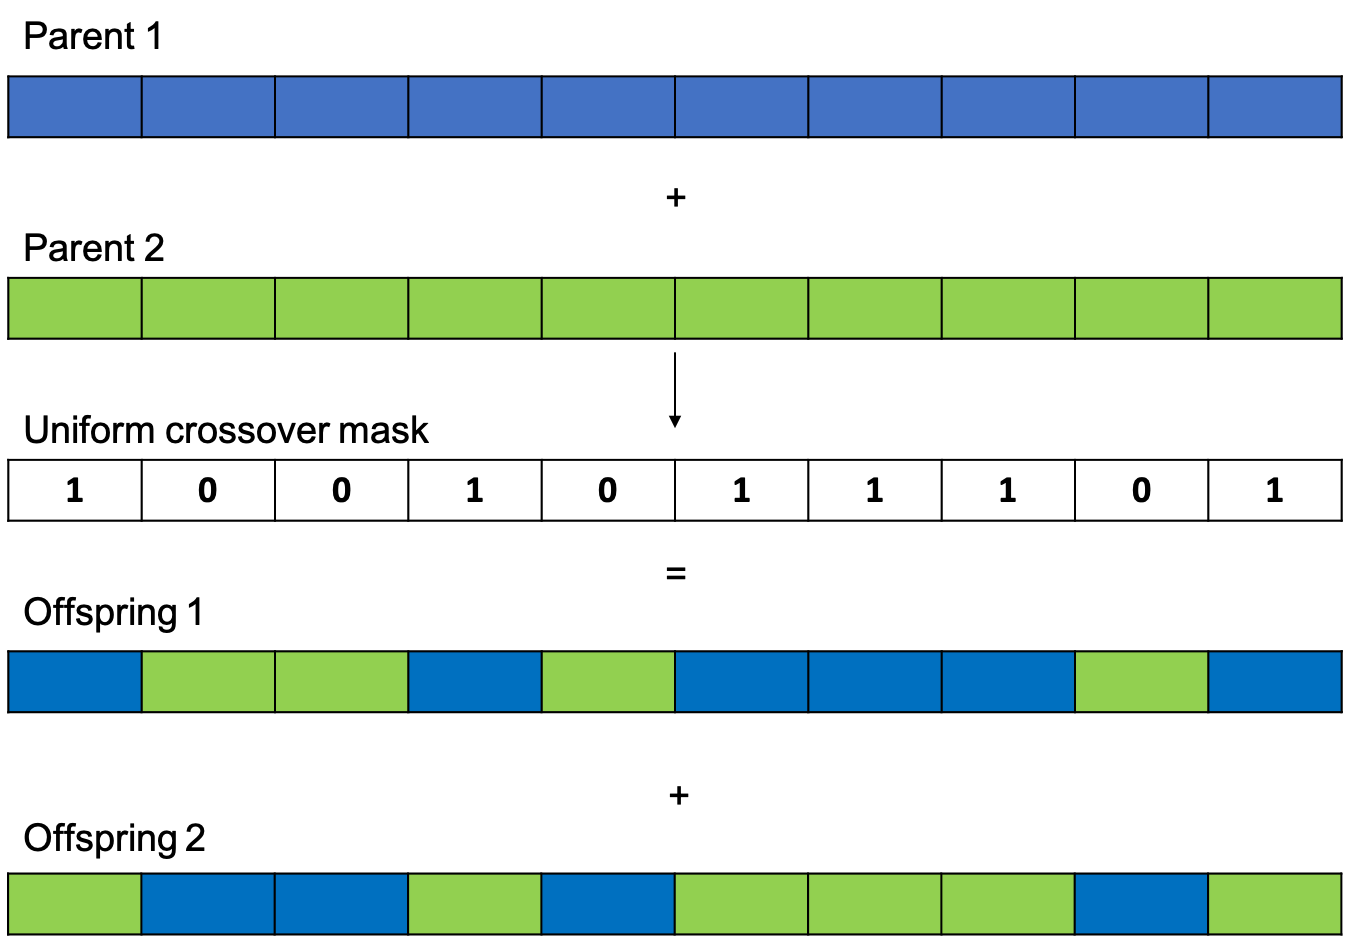
\includegraphics[width=\textwidth]{images/uniform_crossover.png}
      \caption{An illustration of the uniform crossover operator as it applies to sexual recombination, resulting in two new offspring.}
      \label{fig:heuristics:mh:ga:uniform_crossover}
\end{figure}


\begin{algorithm}[H]
      \caption{The pseudo code for the uniform crossover operator as used by \acp{GA}.}
      \label{algo:heuristics:mh:ga:uniform_crossover}
      \begin{algorithmic}
            \State Initialise the mask, $m_{j}(t) = 0 \forall j = 1, \dots, N_{x}$;
            \For{$j = 1$ to $N_{x}$}
            \If{$U(0,1) \leq p_{x}$}
            \State $m_{j}(t) = 1$;
            \EndIf
            \EndFor
            \State
      \end{algorithmic}
\end{algorithm}

In Algorithm~\ref{algo:heuristics:mh:ga:uniform_crossover} above, $p_{x}$ is the bitswapping probability.


\subsubsection{Mutation}
\label{sec:heuristics:mh:ga:mutation}

The mutation operator is applied in order to introduce new genetic material into an existing entity \cite{ref:engelbrecht:2007}. In doing so, diversity is added into the genetic characteristics of the population. Mutation is applied at a certain mutation probability $p_{m}$ to each gene of the offspring $x_{i}(t)$ to produce mutated offspring $x'_{i}(t)$. \citeauthor{ref:engelbrecht:2007}\cite{ref:engelbrecht:2007} mentions that the mutation probability, also referred to as the mutation rate is usually small such that $p_{m} \in [0,1]$ to ensure that good solutions are not distorted too much.

Similar to the crossover operator, mutation operators can be classified according to the representation scheme used. In the context of training
\acp{FFNN}, binary crossover operators such as the \textit{uniform} mutation operator can be used to generate a mutation mask that specifies which genes are mutated. For the purposes of this dissertation, the application of the mutation operator on $x_{ij}(t)$ results in a small update step for that gene such that $x'_{ij}(t) = x_{ij}(t) + v_{ij}(t)$. In this case, $v_{ij}(t) \sim U(-limit, limit)$ and $limit = \sqrt{\frac{6}{fanin + fanout}}$ as presented for Glorot uniform sampling in~\ref{chap:anns}. An adaptation of the uniform mutation operator is then provided in Algorithm~\ref{algo:heuristics:mh:ga:uniform_mutation} below.

\begin{algorithm}[H]
      \caption{The pseudo code for the uniform mutation operator as used by \acp{GA}.}
      \label{algo:heuristics:mh:ga:uniform_mutation}
      \begin{algorithmic}
            \For{$j = 1$ to $N_{x}$}
            \If{$U(0,1) \leq p_{m}$}
            \State Sample update step $v_{ij}(t) \sim U(-limit, limit)$
            \State $x'_{ij}(t) = x_{ij}(t) + v_{ij}(t)$;
            \EndIf
            \EndFor
            \State
      \end{algorithmic}
\end{algorithm}

An illustration of the adapted uniform mutation operator is presented in Figure~\ref{fig:heuristics:mh:ga:uniform_mutation} below.

\begin{figure}[htbp]
      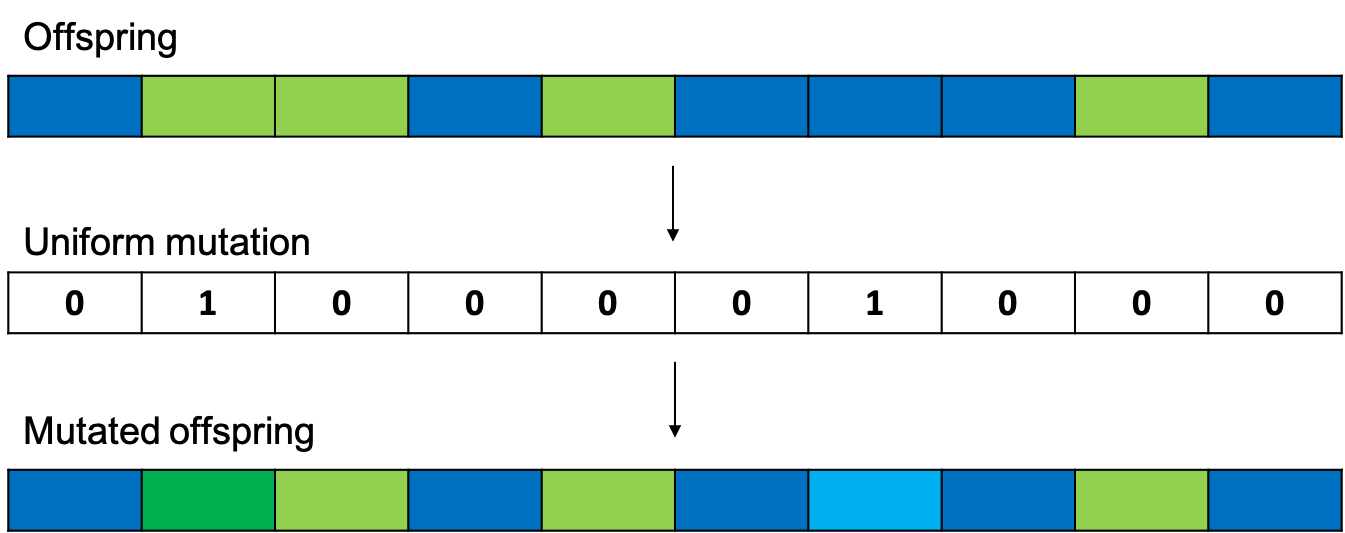
\includegraphics[width=\textwidth]{images/uniform_mutation.png}
      \caption{An illustration of the adapted uniform mutation operator as it applies to mutated offspring.}
      \label{fig:heuristics:mh:ga:uniform_mutation}
\end{figure}

\subsubsection{Selection}
\label{sec:heuristics:mh:ga:selection}

Selection is a widely used concept in all \acp{EA} and models survival of the fittest in the evolutionary context. The main idea behind the selection operator is to emphasise better solutions \cite{ref:engelbrecht:2007}. This is done in two of the main components of \acp{EA}. These include

\begin{itemize}
      \item \textbf{Selection of the new population: } A new population of candidate solutions are is selected at the end of each generation to serve as the population for the next generation. The new population can be selected from both the parents and offspring. The selection operator is thus responsible for ensuring that good entities survive to the next generation.

      \item \textbf{Reproduction: } Offspring is created through the crossover and/or the mutation operators. In terms of crossover, good solutions should have a high probability of reproducing to ensure that offspring contain genetic material of the best entities. In terms of mutation, selection mechanisms should focus on weaker entities. By mutating weak entities, the hope is to introduce better traits, increasing their chance to survive.
\end{itemize}

\citeauthor{ref:engelbrecht:2007}\cite{ref:engelbrecht:2007} mentions that selection operators are characterised by their \textit{selective pressure}. Selective pressure is defined as the speed at which the best entity's solution will occupy the entire population by repeated application of the selection operator alone \cite{ref:back:1994}. A selection operator with a high selective pressure rapidly decreases the diversity in the population. This could lead to premature convergence. A high selective pressure limits the exploration abilities of the population. Similar to other components and operators presented in this chapter, selection mechanisms should maintain a balance between exploration and exploitation.

Various selection mechanisms have been proposed. For the purposes of this dissertation, focus is put on the following selection mechanisms and concepts.

\begin{itemize}
      \item \textbf{Tournament Selection: } Tournament selection selects a group of $N_{ts}$ entities randomly from the population such that $N_{ts} < N_{s}$, where $N_{s}$ is the population size. The performance of the selected $N_{ts}$ entities are then compared and the best entities from this group is selected and returned by the operator. It should be mentioned that for sexual crossover of two parents, tournament selection is applied twice, first for the first parent and the again for the second parent. \citeauthor{ref:engelbrecht:2007}\cite{ref:engelbrecht:2007} mentions that tournament selection prevents the best entities from dominating provided that $N_{ts}$ is not too large. This results in a lower selective pressure. If $N_{ts}$ is too small, the chances that bad entities will be selected increase.

      \item \textbf{Rank-based Selection: } Rank-based selection uses the rank-ordered fitness values to determine the probability of selection and not the absolute fitness value. It can therefore be said that selection is independent of actual fitness values. \citeauthor{ref:engelbrecht:2007}\cite{ref:engelbrecht:2007} mentions that the advantage of this approach is that the best entities will not dominate the selection process. Non-deterministic linear sampling selects an entity $x_{i}(t)$ such that $i \sim U(0, U(0, N_{s} - 1))$. Importantly, in the context of a minimisation problem, entities are first sorted in decreasing order of fitness value, assuming that the best heuristic is then contained at index 0, while the worst entity is contained at index $N_{s} - 1$.

      \item \textbf{Elitism: } Elitism refers to the process of ensuring that the best entities from the current population survive to the next generation. The best entities are simply passed on to the next generation without mutation. The more entities that survive to the next generation, the lower the diversity of the new population. It is later shown in~\ref{chap:bhh} that the proposed \ac{BHH} can incorporate a form of elitism in its credit assignment strategy.
\end{itemize}


\subsubsection{Control Parameters}
\label{sec:heuristics:mh:ga:control_parameters}

Throughout this section a number of control parameters have been provided that affect the performance of the \ac{GA}. These include the population size $N$, the crossover rate $p_{c}$ and the mutation rate $p_{m}$. \citeauthor{ref:engelbrecht:2007}\cite{ref:engelbrecht:2007} mentions that these values are usually kept static. However, it is widely accepted that these parameters have a significant impact on the performance of the \ac{GA}.  Finding optimal values for $p_{c}$ and  $p_{m}$ empirically can be a time consuming process. As such, dynamic parameter values can be introduced, however, this is beyond the scope of this dissertation.


\section{Summary}
\label{sec:heuristics:summary}

This chapter provided the reader with detailed background information on different heuristics that have been shown to be able to train \acp{FFNN}. Two main groups of heuristics where discussed. These include gradient-based heuristics and \aclp{MH}. For each of these groups a number of different variants have been discussed. A total of ten different heuristics have been introduced and where possible, their advantages, disadvantages and characteristics have been discussed.

The next chapter aims to build on the foundations provided in this chapter by putting focus on \acp{HH}. It is shown that \acp{MH} implement a heuristic pool of lower-level heuristics such as those presented in this chapter.











\section{Hyper-Heuristics}
\label{sec:hhs}
\chapter{Probability Test}
\label{chap:probability}

\begin{quotation}
    \textit{I flip the coin in the air. Heads. I flip the coin in the air.
        Tails. I do this, probably hundreds of times, until finally, ten heads
        in a row. Suddenly it hit me. Despite knowing the odds, despite knowing
        that it might take a long time, we still hope, because we know, no
    matter the odds, there is still a chance.}
\end{quotation}

Probability theory finds its application in many fields today ranging from
finance to medicine. It is a powerful tool that allows us to predict the
future, with a certain degree of surity. Probability theory finds its place in
the field of \ac{ML} too. In 1991,
\citeauthor{ref:denker:1991}, \cite{ref:denker:1991} proposed a way to transform
\ac{ANN} outputs to probability distributions . In 1993,
\citeauthor{ref:neal:1993} \cite{ref:neal:1993} developed the first \ac{MCMC}
sampling algorithm for Bayesian \acp{NN}. This shows that probability theory
can be used as a mechanism for learning in \acp{ANN}.

The purpose of this chapter is to provide the necessary background information
needed to understand probability theory as it plays a vital role in the
formulation of the \ac{BHH}.  The chapter is structured as follows:

\begin{itemize}
    \item
    Section~\ref{sec:probability:probability} gives a brief overview of what
    probability is and how it is used.
    
    \item
    Section~\ref{sec:probability:joint_probability} gives a brief overview of
    how probabilities are interpreted for random events that are considered
    jointly.

    \item
    Section~\ref{sec:probability:cond_probability} introduces conditional
    probability. Brief discussions follow on the \textit{frequentist} view
    of conditional probability as well as the \textit{Bayesian} view of
    conditional probability through \textit{Bayes Theorem}.

    \item
    Section~\ref{sec:probability:likelihood} gives a brief overview of the
    concept of likelihood. A brief discussion follow on how likelihood is used
    alongside probability.

    \item
    Section~\ref{sec:probability:probability_distributions} presents relevant
    probability distributions, including the \index{beta
    distribution}\textit{beta} distribution, the \index{dirichlet
    distribution}\textit{dirichlet} distribution, the \index{bernoulli
    distribution}\textit{bernoulli} distribution, the \index{binomial
    distribution}\textit{binomial} distribution, the \index{categorical
    distribution}\textit{categorical} distributions, and the \index{multinomial
    distribution}\textit{multinomial} distribution.

    \item
    Section~\ref{sec:probability:conjugate_priors} presents the conjugate prior
    probability distributions for the \index{bionomial likelihood}binomial
    likelihood as well as the \index{categorical likelihood}\index{multinomial
    likelihood}categorical/multinomial likelihood.

    \item
    Section~\ref{sec:probability:bayesian_stats} presents \textit{Bayesian}
    statistics. It is shown how Bayes' Theorem can be used as an inferencing
    mechanism. Detailed discussions follow on \index{Bayesian
    optimisation}Bayesian optimisation methods such as \index{Bayesian
    inference}\textit{Bayesian inference} and \index{Bayesian analysis}\textit{Bayesian analysis}.

    \item
    Finally, a brief summary of the chapter is given in
    Section~\ref{sec:probability:conclusion}.
\end{itemize}

\section{Probability}
\label{sec:probability:probability}

In everyday conversation, the term \textit{probability} is a measure of one's
belief in the occurrence of a future event \cite{ref:wackerly:2014}.
Consider flipping an unbiased, fair coin. One could consider the probability of
an outcome, whether it is heads or tails, to be a ratio of the possible number
of outcomes. In the case of a coin, the number of outcomes is just two. This
means that one can \textit{believe} that the coin would land with the head-side
up with $1/2$ odds.

Probability can be inferred and confirmed through past events. The support of
these inferred probabilities get stronger as more and more samples of
independent random events, such as flipping of a fair coin, are gathered.  In
the case of flipping a fair coin, the \ac{CLT} shows that the normalised sum of
events tends toward a normal distribution with a mean value of $0.5$ if the
number of events observed $n$ is large (usually $n \geq 30$)
\cite{ref:wackerly:2014}. This shows that the probability of the coin landing
on heads is $50\%$. An illustration of a coin flipping simulation that shows
the central limit theorem on various sample sizes is provided below:

\begin{figure}[ht]
    \centering
    \begin{subfigure}[b]{0.5\textwidth}
        \centering
        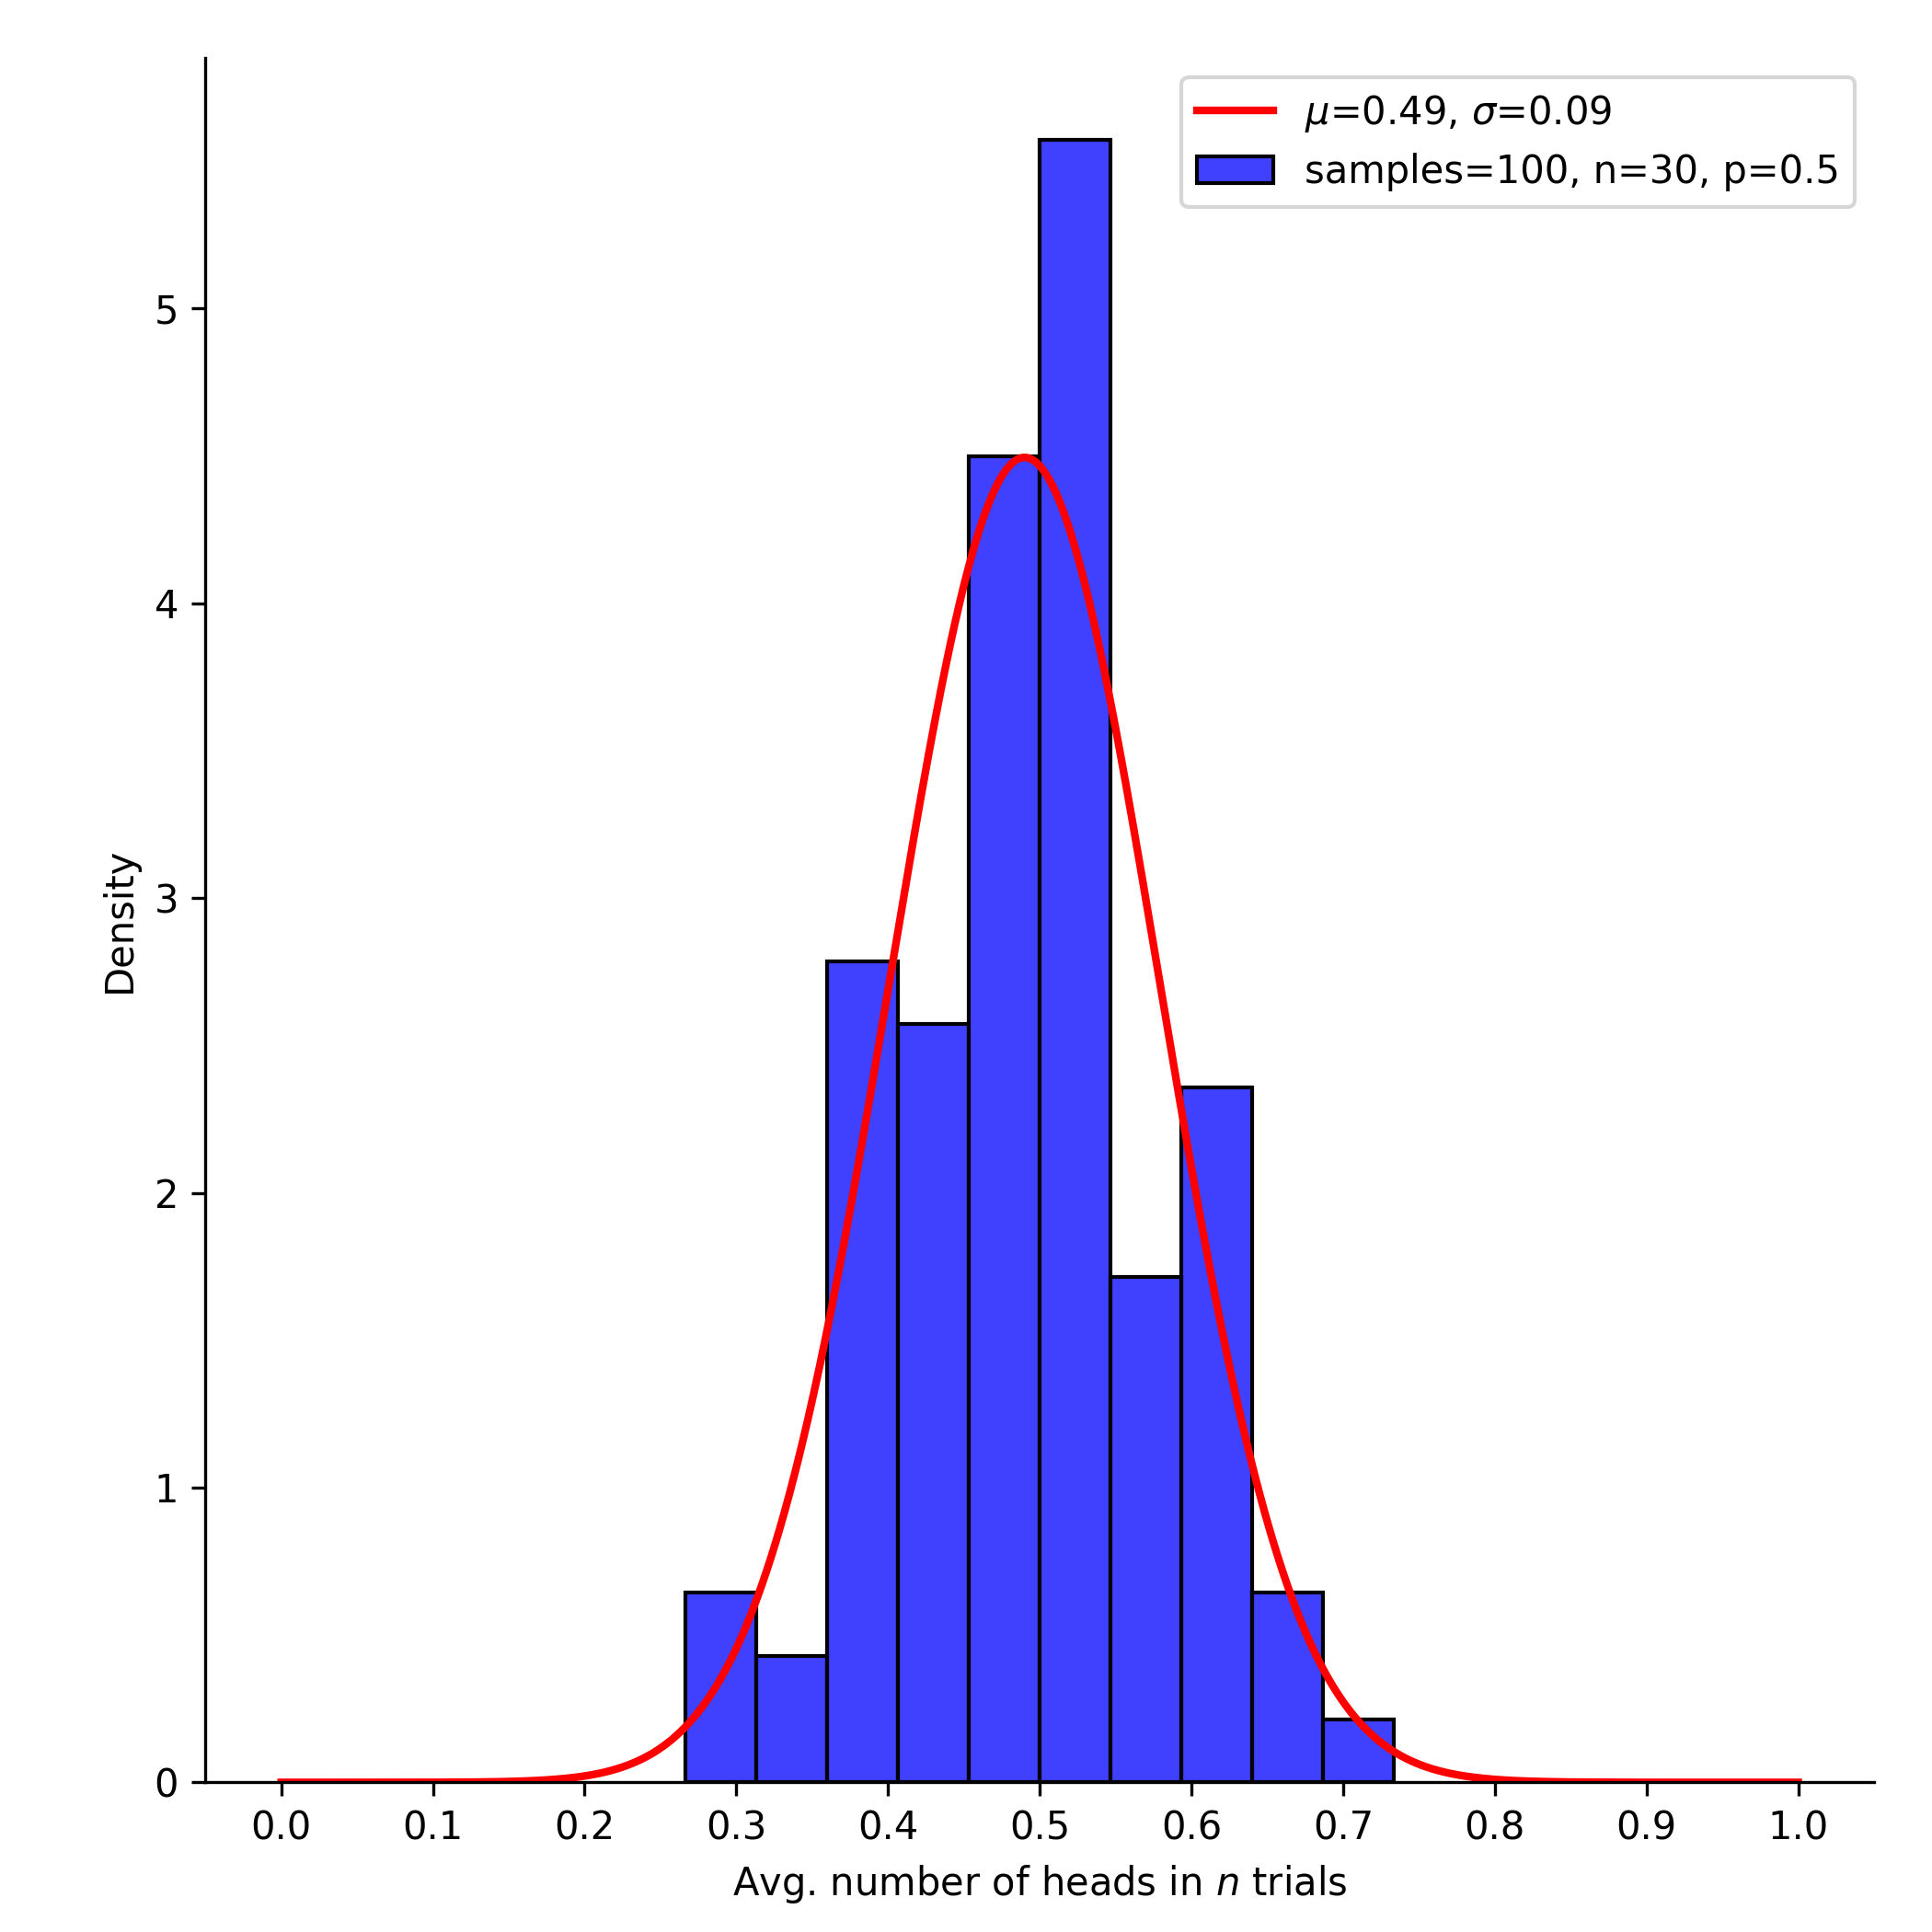
\includegraphics[width=\textwidth]{coin_flip_samples_100.png}
        \caption[Coin flip simulation. Samples=100]{100 samples}
        \label{fig:coin_flip_simulation_samples_100}
    \end{subfigure}
    \hfill
    \begin{subfigure}[b]{0.5\textwidth}
        \centering
        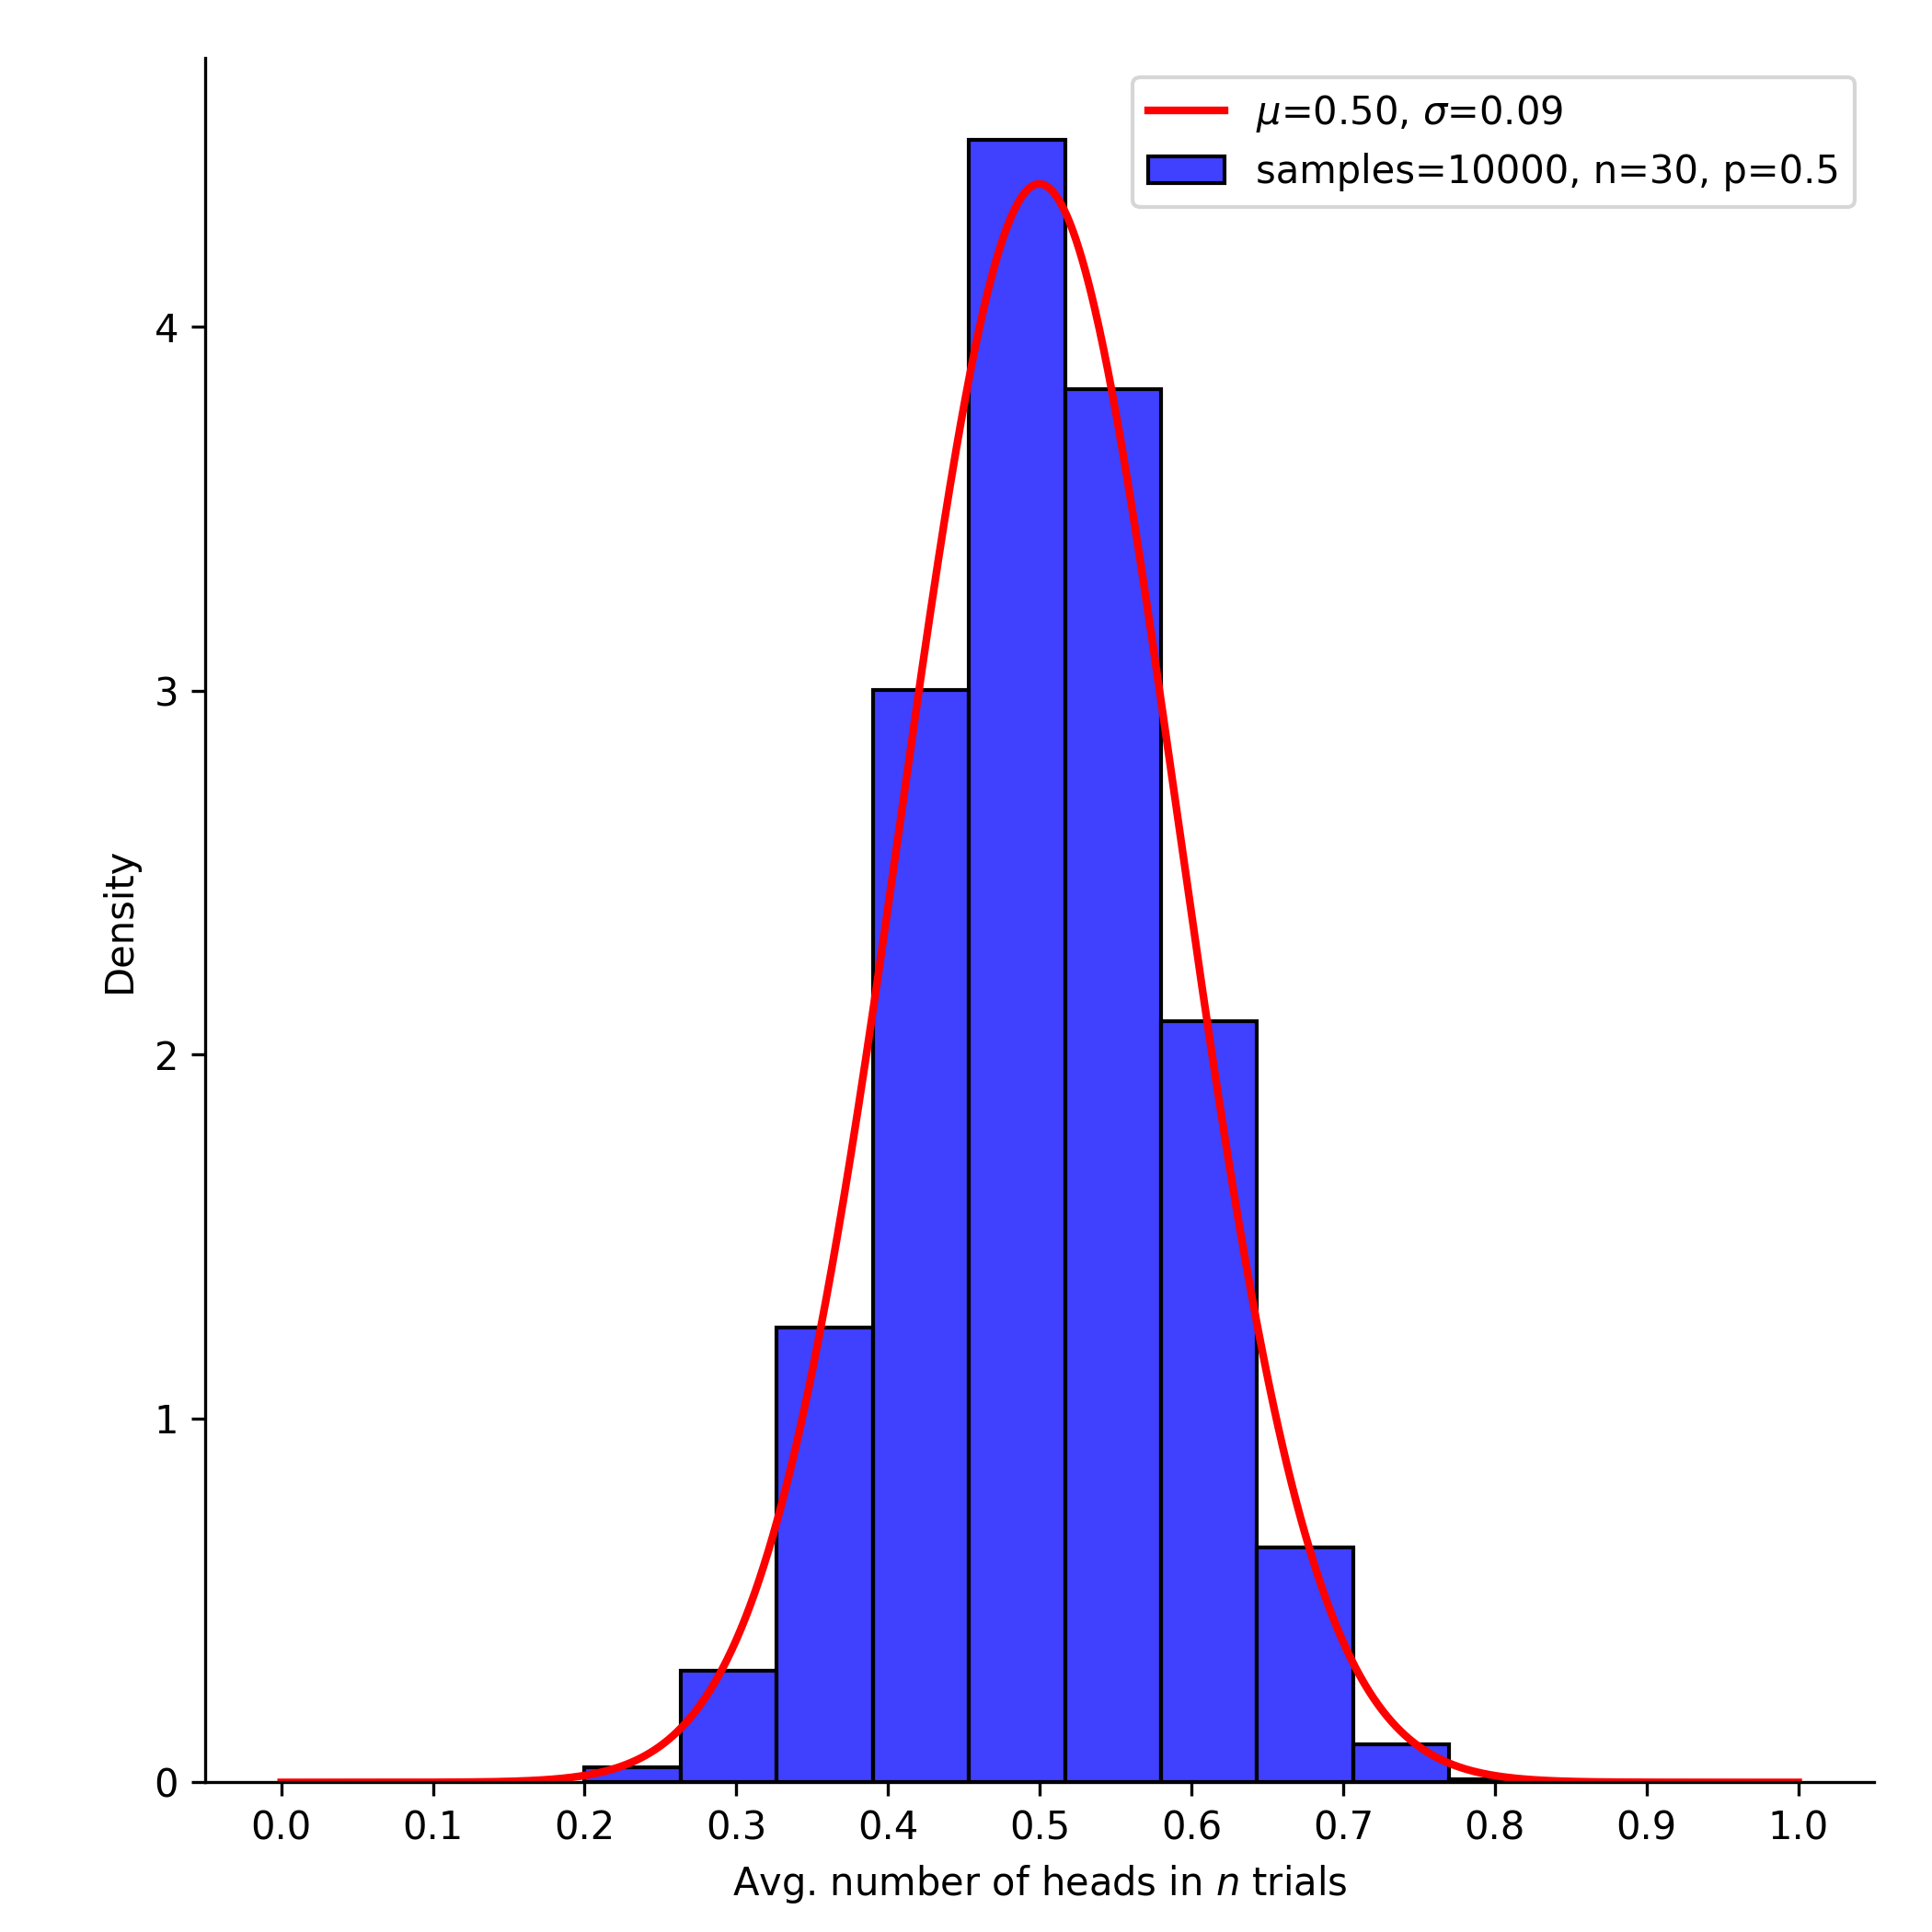
\includegraphics[width=\textwidth]{coin_flip_samples_10000.png}
        \caption[Coin flip simulation. Samples=100]{10000 samples}
        \label{fig:coin_flip_simulation_samples_10000}
    \end{subfigure}
    \caption{An illustration of the \index{central limit theorem}central limit theorem on a coin flip simulation}
    \label{fig:coin_flip_simulation}
\end{figure}








\section{Joint Probability}
\label{sec:probability:joint_probability}












\section{Conditional Probability}
\label{sec:probability:cond_probability}












\subsection{Frequentist}
\label{sec:probability:cond_probability:frequentist}












\subsection{Bayes Theorem}
\label{sec:probability:cond_probability:bayes_theorem}












\section{Likelihood}
\label{sec:probability:likelihood}












\section{Probability Distributions}
\label{sec:probability:probability_distributions}












\subsection{Beta Distribution}
\label{sec:probability:probability_distributions:beta}

The Beta distribution is a family of univariate continuous probability distributions over some $x$, with support on the interval $[0,1]$. It is parametrised by two shape parameters $\alpha > 0, \alpha \in \mathbb{R}$ and $\beta > 0, \beta \in \mathbb{R}$. The Beta distribution is denoted as $Beta(\alpha, \beta)$. The  PDF of the Beta distribution is given below as:

\begin{equation}
P(x | \alpha, \beta) = f_{Beta}(x; \alpha, \beta) = \frac{1}{B(\alpha, \beta)} x^{\alpha - 1} (1 - x)^{\beta - 1}
\end{equation}

where the normalising  constant $B(\alpha, \beta)$ is defined as:

\begin{equation}
B(\alpha, \beta) = \frac{\Gamma(\alpha)\Gamma(\beta)}{\Gamma(\alpha + \beta)}
\end{equation}

and $\Gamma$ is the Gamma function as defined below:

\begin{equation}
\Gamma(n) = ( n - 1)!
\end{equation}

The Gamma function can also be written as:

\begin{equation}
\Gamma(n+1) = n!
\end{equation}

If should be noted that $\alpha$ and $\beta$ determine the shape of the distribution. There exists a special case when $\alpha = \beta$. This is referred to as the symmetric Beta distribution. In the case where $\alpha = \beta = 1$ the distribution is equivalent to the uniform distribution over all points in its support. The Beta distribution for various values of $\alpha$ and $\beta$, including the symmetric version is presented below in figures (???):

INSERT FIGURE HERE.

The expected value of $x$ is given below as:

\begin{equation}
E[x] = \frac{\alpha}{\alpha + \beta}
\end{equation}

Similarly, the expected value of the natural logarithm of $x$ can be calculated as shown below:

\begin{equation}
E[\ln(x)] = \psi({\alpha}) - \psi(\alpha + \beta)
\end{equation}

where $\psi$ is the logarithmic derivative of the Gamma function, called the Digamma function. The Digamma function is defined below as:

\begin{equation}
\psi(n) = \frac{d}{dn}\ln(\Gamma(n)) = \frac{\Gamma'(n)}{\Gamma(n)}
\end{equation}

Finally, the mode of the distribution is given below as:

\begin{equation}
Mo[x] = E[x] - 1 = \frac{\alpha - 1}{\alpha + \beta - 1}
\end{equation}










\subsection{Dirichlet Distribution}
\label{sec:probability:probability_distributions:dirichlet}


The Dirichlet distribution is a family of multivariate continuous probability distributions over some $x$ in $K$ dimensions. The Dirichlet distribution is the multivariate generalization of the Beta distribution and is thus sometimes referred to by its alternative name, the Multivariate Beta Distribution (MBD). The Dirichlet distribution is parametrised by some vector $\alpha = (\alpha_{1}, \dots, \alpha_{K}), \forall_{k=1}^{K} \alpha_{k} > 0, \alpha_{k} \in \mathbb{R}$. $\alpha$ is referred to as the  concentration parameter. The Dirichlet distribution of order $K \geq 2$ with parameters $\alpha$, denoted $Dir(\alpha)$, has a PDF as given below:

\begin{equation}
P(x | \alpha) =  f_{Dir}(x; K, \alpha) = \frac{1}{B(\alpha)}  \prod_{k=1}^{K} x_{k}^{\alpha_{k} - 1}
\end{equation}

where the normalising constant $B(\alpha)$ is defined as:

\begin{equation}
B(\alpha) = \frac{\prod_{k=1}^{K} \Gamma(\alpha_{k})}{\Gamma(\alpha_{0})}
\end{equation}

and $\alpha_{0}$ is defined as:

\begin{equation}
\alpha_{0} = \sum_{k=1}^{K}\alpha_{k}
\end{equation}

Importantly, the set $\{x_{k}\}_{k=1}^{K}$ belongs to the standard $K-1$ probability simplex $S$, meaning that $x_{K} = 1 - \sum_{k=1}^{K-1}x_{k}$ with support $\forall_{k=1}^{K} x \in [0,1]$. Under the simplex $S$, this means that the sum over all values of the vector $x$ must be 1. The simplex can thus be rewritten as $\sum_{k=1}^{K}x_{k} = 1$.

Similar to the Beta distribution, $\alpha$ determines the shape of the distribution in $K$ dimensions and thus, there also exist a special case, referred to as the symmetric distribution when $\forall_{k=1}^{K} \alpha_{k} = c$, where $c$ is some constant. In the case where $c = 1$, the distribution is referred to as a flat distribution and yields the uniform distribution over all points in $S$. The Dirichlet distribution of order $K = 3$, for various values of $\alpha$ , including the symmetric version is presented in figures (???) below:

INSERT FIGURE HERE.


The expected value of $x$ is given below as:

\begin{equation}
E[x_{k}] = \frac{\alpha_{k}}{\alpha_{0}}
\end{equation}

Similarly, the expected value of the natural logarithm of $x_{k}$ can be calculated as follows:

\begin{equation}
E[\ln(x_{k})] = \psi({\alpha_{k}}) - \psi(\alpha_{0})
\end{equation}


where $\psi$ is the Digamma function as defined in Equation (???). Finally, the mode of the distribution is given as:

\begin{equation}
\begin{split}
	Mo[x_{k}] &= E[{x_{k}] -K^{-1}} \\
		&=  \frac{\alpha_{k} - 1}{\alpha_{0} - K}
\end{split}
\end{equation}













\subsection{Bernoulli Distribution}
\label{sec:probability:probability_distributions:bernoulli}

The Bernoulli distribution is a discrete probability distribution over some random variable $x$ that takes the value of $1$ with probability $\theta$ and $0$ with probability $1-\theta$. It is denoted as $Ber(\theta)$ with support $x \in \{0, 1\}$. In probability theory, the Bernoulli distribution is often used to explain the possible outcomes of a single experiment that asks a \textit{yes-no} question such as flipping a coin (ref ???). The outcome of such an experiment is a boolean value. The Bernoulli distribution has a PMF as given below:

\begin{equation}
P(x | \theta) = f_{Ber}(x; \theta) =
	\begin{cases}
		\theta & \text{if}\ x=1 \\
      	1 - \theta & \text{if}\ x=0
	\end{cases}
\end{equation}

The above equation can also be expressed as:

\begin{equation}
f_{Ber}(x; \theta) = \theta^{x}(1-\theta)^{1-x}
\end{equation}

% (See 3rd paragraph: $https://en.wikipedia.org/wiki/Central_limit_theorem$???). 
\todo[inline]{See comment in code}
The mean of the Bernoulli distribution approaches $\theta$ over many samples as
explained in the Central Limit Theorem The expected value of the distribution is thus given as:

\begin{equation}
E[x] = \theta
\end{equation}

while the mode of the distribution is given as:

\begin{equation}
Mo[x_{k}] = 
\begin{cases}
	0 & \text{if}\ \theta < 0.5 \\
    	0,1 & \text{if}\ \theta = 0.5 \\
    	1 & \text{if}\ \theta > 0.5 \\
\end{cases}
\end{equation}




\subsection{Binomial Distribution}
\label{sec:probability:probability_distributions:bin}


The Binomial distribution is a discrete probability distribution over a random variable $x$ taking on a number of successes, in $N$ sequential independent experiments that each ask a \textit{yes-no} question. The probability of a single independent experiment yielding a success is given as $\theta$ and the Binomial distribution is denoted as $Bin(N, \theta)$ with support $x \in \{0, 1, \dots, N\}$.  It should be noted that the Binomial distribution is the extension of the Bernoulli distribution over $N$ independent sequential experiments and thus, each experiment also yields some boolean outcome. When $N=1$, the experiment is referred to as a Bernoulli trial and the distribution is just a Bernoulli distribution and when $N > 1$, the sequence of outcomes is referred to as a Bernoulli process. The PMF of the Binomial distribution is given as follows:

\begin{equation}
    P(x \vert \theta; N) = f_{Bin}(x; N, \theta) = \binom{N}{x} \theta^{x}(1-\theta)^{1-x}
\end{equation}

The mean of the Binomial distribution is just $N\theta$ given the Central Limit Theorem (See paragraph 3 $https://en.wikipedia.org/wiki/Central_limit_theorem$ ???). The expected value of the Binomial distribution is thus given as:

\begin{equation}
E[x] = N\theta
\end{equation}

while the mode of the distribution is given as:

\begin{align}
\begin{split}
Mo[x_{k}] &= E[x] + \theta \\
	&= N\theta  + \theta \\
	&= (N  + 1)\theta
\end{split}
\end{align}



\subsection{Categorical Distribution}
\label{sec:probability:probability_distributions:categorical}

The Categorical distribution is a discrete probability distribution over some random variable $x$, taking on any one of $K$ possible categories. There is no innate underlying ordering to these categories, so for simplicity, each category is assigned a numerical representative value such that $k = (1, \dots, K)$. The probabilities for all outcomes is given by the probability vector $\theta = (\theta_{1}, \dots, \theta_{K})$.  This means that the probability $P(x=k)=\theta_{k}$, with support $x \in \{1, \dots, K\}$. The Categorical distribution, denoted $Cat(\theta)$ is the generalization of the Bernoulli distribution and is sometimes referred to it by its alternative names, the Generalized Bernoulli Distribution (GBD) or the Multinoulli distribution. In probability theory, the Categorical distribution is often used to explain the outcome of a single experiment with more than two possible outcomes such as rolling a die (ref ??). The PMF of the Categorical distribution is given as:

\begin{equation}
P(x | \theta; K) = f_{Cat}(x; K, \theta) = \prod_{k=1}^{K}\theta_{k}^{[x = k]}
\end{equation}

where $[x = k]$ is the Iversion Bracket (ref ???), yielding 1 if $x = k$ and 0 otherwise. From this, one can conclude that:

\begin{equation}
f_{Cat}(x=k; K, \theta) = \theta_{k}
\end{equation}

The random variable $x$ can also be encoded in binary format, yielding a vector $x = (x_{1}, \dots, x_{K})$ of Bernoulli distributions such that the support is $\forall_{k=1}^{K} x_{k} \in \{0, 1\}$. Importantly, if the outcome of the random event is of category $k$, then $x_{k} = 1$ and $\forall_{j=1}^{K} x_{j} = 0, j \neq k$ so that the standard $K-1$ probability simplex $S$ still holds. The PMF of the Categorical distribution can then be rewritten as follows:

\begin{equation}
f_{Cat}(x; K, \theta) = \prod_{k=1}^{K}\theta_{k}^{\mathbbm{1}_{1}(x_{k})}
\end{equation}

where $\mathbbm{1}(x_{k})$ is the Indicator Function, yielding 1 if $x_{k} = 1$ and 0 otherwise.

Since there is no innate order to the underlying categories, the mean of the distribution does not yield any relevant information (ref??). The mode of the distribution is given below as:

\begin{equation}
Mo[x] = \argmax_{k}(\theta_{1}, \dots, \theta_{K})
\end{equation}


\subsection{Multinomial Distribution}
\label{sec:probability:probability_distributions:multinomial}

The Multinomial distribution is a discrete probability distribution over some random variable $x = (x_{1}, \dots\, x_{K})$ that takes on the counts for each occurrence of $K$ possible classes in $N$ independent trials. The probabilities for all possible outcomes in a single trial is given by the probability vector $\theta = (\theta_{1}, \dots, \theta_{K})$. The Multinomial distribution, denoted $Mul(N, K, \theta)$, is thus the generalization of the Binomial distribution to $K$ dimensions. Note that when:

\begin{itemize}
	\item When $K$ is 2 and $N = 1$, the Multinomial distribution is the Bernoulli distribution.
	\item When $K$ is 2 and $N > 1$, the Multinomial distribution is the Binomial distribution.
	\item When $K > 2$ and $N = 1$, the Multinomial distribution is the Categorical distribution.
\end{itemize}
  
The support for the Multinomial is $\forall_{i=1}^{K} x_{k} \in \{1, \dots, N\}, \sum_{k=1}^{K}x_{k} = N$ and the PMF for the Multinomial distribution is given as:

\begin{equation}
P(x | \theta; N; K) = f_{Mul}(x; N, K, \theta) = \frac{N!}{\prod_{k=1}^{K}x_{k}!} \prod_{k=1}^{K}\theta_{k}^{x_{k}}
\end{equation}

Similar to the Categorical distribution, the random variable $x$ can also be encoded in binary format, yielding an $N \times K$ matrix $X$ of Bernoulli distributions. The support is then given as $X \in \{0, 1\}^{N \times K}, \forall_{i=1}^{N}\sum_{k=1}^{K} x_{i,k} = 1$ so that the standard $K-1$ probability simplex $S$ still holds for each trial. The PMF of the Multinomial distribution can then be rewritten as follows:

\begin{equation}
\begin{split}
f_{Mul}(x; N, K, \theta) &= \frac{N!}{\prod_{k=1}(\sum_{i=1}^{N}x_{i, k})!}\prod_{i=1}^{N}\prod_{k=1}^{K}\theta_{k}^{\mathbbm{1}_{1}(x_{i,k})} \\
	&= \frac{N!}{\prod_{k=1}(\sum_{i=1}^{N}x_{i, k})!} \prod_{k=1}^{K}\theta_{k}^{\sum_{i=1}^{N}\mathbbm{1}_{1}(x_{i,k})} \\
	&= \frac{N!}{\prod_{k=1}(\sum_{i=1}^{N}x_{i, k})!} \prod_{k=1}^{K}\theta_{k}^{N_{k}} \\
\end{split}
\end{equation}

where $N_{k}$ is a summary variable denoting the number of times a category $k$ occurs over all trials in $N$. The reason why the Categorical and Multinomial distributions are presented as binary encoded vectors is to simplify the proof of their conjugate priors as will be shown next. This is further supported by the fact that NNs often use binary encoding of feature vectors. The combination of these probabilitic methods and NNs forms the basic of this research dissertation.






\section{Conjugate Priors}
\label{sec:probability:conjugate_priors}












\subsection{Binomial Likelihood}
\label{sec:probability:conjugate_priors:binom_likelihood}

The conjugate prior to a Bernoulli distribution is the Beta distribution
(ref???). This is shown by demonstrating that the posterior distribution has the
same functional form $\mathcal{A}(v)$ as the prior distribution as follows: \\
\textbf{Setup}:

\begin{itemize}
	\item Let $I$ be a number of independent, identical  (iid) random events.
	\item Let $\alpha \in \mathbb{R}, \alpha > 0$ and $\beta \in \mathbb{R}, \beta >0$ be the shape parameters to the Beta distribution.
	\item Let $\theta$ be the probability of a success. With $\theta | \alpha, \beta \sim Beta(\alpha, \beta)$.
	\item $P(\theta)$ is the prior probability distribution with the functional form $\mathcal{A}(v)$.
	\item Let $X = (x_{1}, \dots, x_{I})$ be the outcomes of independent, identical random events, each with boolean outcome. That is $x_{i} | \theta \overset{\text{iid}}{\sim} Ber(\theta)$ and thus $\mathcal{L}(x_{i} \vert \theta)$ is the Bernoulli log likelihood.
	\item Let $\mathcal{D}$ denote all the prior data $X, \alpha, \beta$.
	\item Let $N_{1} = \sum_{i=1}^{I} \mathbbm{1}(x_{i} = 1)$ and $N_{0} = \sum_{i=1}^{I} \mathbbm{1}(x_{i} = 0)$.
	\item  The likelihood of the Bernoulli distribution is:
	
\begin{equation}
\begin{split}
	\mathcal{L}(\mathcal{D}) &=  P(\mathcal{D} | \theta) \\
	&\propto \theta^{N_{1}}(1-\theta)^{N_{0}}
\end{split}
\end{equation}

\end{itemize}

\textbf{Then}:

\begin{itemize}
	\item  By Bayes Theorem, the posterior distribution with given prior data $\mathcal{D}$ is given as:
	
\begin{equation}
\begin{split}
	P(\theta | \mathcal{D}) &= \frac{P(\mathcal{D} | \theta) P(\theta)}{P(\mathcal{D})}
\end{split}
\end{equation}

	\item Since the denominator sums to $1$, one could get rid of the denominator and constants for the Bernoulli likelihood and the Beta prior, by expressing the posterior as proportional to:

\begin{equation}
\begin{split}
		P(\theta | \mathcal{D}) &\propto \left[\theta^{N_{1}}(1-\theta)^{N_{0}}\right] \left[\theta^{\alpha - 1} (1 - \theta)^{\beta - 1}\right] \\
		&\propto \theta^{(N_{1} + \alpha) - 1}(1-\theta)^{(N_{0} + \beta) - 1} \\
		&\propto Beta(N_{1} + \alpha, N_{0} + \beta) 
\end{split}
\end{equation}

\item Yielding a posterior of the same functional form $\mathcal{A}(v)$ as the prior, but with updated prior parameters $\alpha' = N_{1} + \alpha$ and $\beta' = N_{0} + \beta$.

\end{itemize}

This shows that the Beta distribution is the conjugate prior to the Bernoulli likelihood.

Furthermore, it should be noted now that this updating of one's prior beliefs by new evidence as shown above forms the basis for this entire research dissertation. (<<Mention something here about the quote from the master algorithm) >> This is shown in more detail in Chapter (???), however, for now, let us now consider the conjugate prior to the Categorical and Multinomial distributions.











\subsection{Categorical and Multinomial Likelihood}
\label{sec:probability:conjugate_priors:cat_mult_likelihood}

The conjugate prior to a Categorical and Multinomail distribution is the Dirichlet distribution (ref???). Similar to the proof of the conjugate prior for the Bernoulli distribution as shown above, this means that the posterior distribution must have the same functional form $\mathcal{A}(v)$ as the prior distribution. This is shown as follows: \\
\textbf{Setup}:

\begin{itemize}
	\item Let $I$ be a number of independent, identical (iid) random events.
	\item Let $K$ be a number of possible outcomes for each event, with $K \geq 2$.
	\item Let $\alpha = (\alpha_{1}, \dots, \alpha_{K}), \forall_{k=1}^{K} \alpha_{k} \in \mathbb{R}, \alpha_{k} > 0$ be the concentration parameters to the Dirichlet distribution.
	\item Let $\theta = (\theta_{1}, \dots, \theta_{K}), \forall_{k=1}^{K} \theta{k} \in (0,1), \sum_{k}^{K} \theta{k} = 1$ be the probability of each class in $K$ and $\theta$ belongs to the standard $K-1$ probability simplex $S$. With $\theta | \alpha \sim Dir(K, \alpha)$. 
	\item $P(\theta)$ is the prior probability distribution with the functional form $\mathcal{A}(v)$.
	\item Let $X = (x_{1}, \dots, x_{I})$ be the outcomes of independent, identical random events, each with $K$ possible outcomes. That is $x_{i} | \theta \overset{\text{iid}}{\sim} Cat(\theta)$ and thus $\mathcal{L}(x_{i} \vert \theta)$ is the Categorical log likelihood.
	\item Let $\mathcal{D}$ denote all the prior data $X, \alpha$.
	\item Let $N = (N_{1}, \dots, N_{K}), N_{k} = \sum_{i=1}^{I} \mathbbm{1}(x_{i,k} = 1)$, denote the counts for each occurrence of a class $k$.
	\item The likelihood of the Categorical and Multinomial distributions is:
	
\begin{equation}
\begin{split}
	\mathcal{L}(\mathcal{D}) &=  P(\mathcal{D} | \theta) \\
	&\propto \prod_{k=1}^{K} \theta_{k}^{N_{k}}
\end{split}
\end{equation}
\end{itemize}

\textbf{Then}:

\begin{itemize}
	\item  By Bayes Theorem, the posterior distribution with given prior data $\mathcal{D}$ is given as:
	
\begin{equation}
\begin{split}
	P(\theta | \mathcal{D}) &= \frac{P(\mathcal{D} | \theta) P(\theta)}{P(\mathcal{D})}
\end{split}
\end{equation}

	\item Since the denominator sums to $1$, one could get rid of the denominator and constants for the Dirichlet prior, by expressing the posterior as proportional to:

\begin{equation}
\begin{split}
		P(\theta | \mathcal{D}) &\propto \prod_{k=1}^{K} \theta_{k}^{N_{k}} \prod_{k=1}^{K} \theta_{k}^{\alpha_{k} - 1}\\
		&\propto \prod_{k=1}^{K} \theta_{k}^{(N_{k} + \alpha_{k}) - 1} \\
		&\propto Dir(K, N + \alpha) 
\end{split}
\end{equation}

\item Yielding a posterior of the same form $\mathcal{A}(v)$ as the prior, but with updated prior parameters $\alpha' = N + \alpha$.

\end{itemize}

This shows that the Dirichlet distribution is the conjugate prior to the Categorical and Multinomial likelihood.









\section{Bayesian Statistics}
\label{sec:probability:bayesian_stats}












\subsection{Bayesian Inference}
\label{sec:probability:bayesian_stats:bayesian_inference}












\subsection{Bayesian Analysis}
\label{sec:probability:bayesian_stats:bayesian_analysis}












\section{Conclusion}
\label{sec:probability:conclusion}




\chapter{Bayesian Hyper-Heuristic}
\label{chap:bhh}

\begin{quote}
      \textit{
            ``The result is a posterior distribution which the agent may use as its new prior in the next step.'' - Pedro Domingos, The Master Algorithm: How the Quest for the Ultimate Learning Machine Will Remake Our World.
      }
\end{quote}

The above quote was the inspiration for the development of a novel \ac{HH} that uses \index{Bayesian}\textit{Bayesian} probability concepts as a selection mechanism to drive the heuristic selection process. Thus far the reader was presented with all of the necessary background information on \acp{ANN} in Chapter \ref{chap:anns}, low-level \index{heuristic}heuristics/\index{Optimiser}optimisers in Chapter \ref{chap:heuristics}, \acp{HH} in Chapter \ref{chap:hhs}  and lastly, \index{probability theory}probability theory in Chapter \ref{chap:probability}. These elements form the fundamental components that make up the proposed \Ac{BHH}. A detailed specification on the \Ac{BHH} can now be formulated. This chapter provides the detail around the theory, concept and implementation of the \Ac{BHH} and explains how it used to train \acp{ANN}. It is shown throughout this chapter that the \Ac{BHH} implements a probabilistic optimisation technique that implements and biases a \index{Gaussian Process}\textit{Gaussian process} towards good optimisation and performance. The remainder of the chapter is structured as follows:

\begin{itemize}
      \item \textbf{Section \ref{sec:bhh:overview}} provides a brief overview of the \Ac{BHH} optimiser.

      \item \textbf{Section \ref{sec:bhh:architecture}} presents the general architecture, \Ac{HH} framework and the various components that make up the \index{Optimiser}optimiser.

      \item \textbf{Section \ref{sec:bhh:heuristic_pool}} discusses the collection of low-level \index{heuristic}heuristics, referred to as the \index{heuristic}\textit{heuristic pool} and puts emphasis on the importance of a diverse set of low-level \index{heuristic}heuristics.

      \item \textbf{Section \ref{sec:bhh:entity_pool}} discusses the detail of the \index{Population}population and its \index{entity}entities, with specific detail provided on entity (local) and population (global) state and memory.

      \item \textbf{Section \ref{sec:bhh:initialisation_step}} presents the initialisation strategy in detail.

      \item \textbf{Section \ref{sec:bhh:selection_mechanism}} presents the \index{Bayesian}\textit{Bayesian} probabilistic model that is used as a selection mechanism.

      \item \textbf{Section \ref{sec:bhh:heuristic_entity_selections}} discusses heuristic-entity selections and how these two concepts are utilised together.

      \item \textbf{Section\ref{sec:bhh:model}} discusses the models that can be optimised using the \Ac{BHH}, specifically referring to its application to training \acp{FFNN}.

      \item \textbf{Section \ref{sec:bhh:train_test_datasets}} briefly discussed the role of the train and test datasets during training.

      \item \textbf{Section \ref{sec:bhh:loss_function}} discusses model evaluation and the role of the loss/cost function.

      \item \textbf{Section \ref{sec:bhh:domain_barrier}} discusses the domain barrier that exists between the high-level \ac{BHH} and low-level heuristics in the \index{heuristic pool}heuristic pool.

      \item \textbf{Section \ref{sec:bhh:performance_log}} presents the performance log and discusses performance measurement in more detail.

      \item \textbf{Section \ref{sec:bhh:credit_assignment_strategy}} discussed credit assignment and move acceptance strategies in detail.

      \item \textbf{Section \ref{sec:bhh:optimisation_step}} presents the learning mechanisms by which the probabilistic model can be optimised.

      \item \textbf{Section \ref{sec:bhh:hyper_parameters}} summarises and discusses the associated \index{hyper-parameters}hyper-parameters and default values.

      \item The pseudo-code algorithm for the \ac{BHH} is given in \textbf{Section \ref{sec:bhh:algorithm}}.

      \item Finally, a summary of the chapter is provide in \textbf{Section \ref{sec:bhh:summary}}.
\end{itemize}


\section{Overview}
\label{sec:bhh:overview}

This section provides an overview of the workings of the \Ac{BHH}. To start the discussion, consider the following analogy:\\
\\
\textit{
      Bob is a teacher at a high school. Every year his students perform really well and he wins the prize for best teacher, evaluated by student performance. He is able to do this not just because he is a good teacher, but he understands that each student has a learning technique that works best for him/her. He exploits this concept by tailoring the teaching process to each students such that the result is an optimum mark for that student and by definition, the whole class. Bob knows that it is too timely to get to know each student, so he devises a model that does the allocations for him. This model uses a process of observation. With each evaluation opportunity he experiments by allocating different learning techniques to different students. He evaluates the student for the given opportunity and keeps a log of which learning technique he assigned to the student as well as the outcome. With each evaluation opportunity he updates his model by biasing the assignment process such that students generally get assigned learning techniques that yield the best performance for them.
}\\
\\
The key take-out from the analogy above is the concept that Bob can maximise student performance by updating his beliefs, over time, about which learning technique to assign to which (type of) student. He does this by biasing selection/assignment towards the best combinations of student, learning technique
and evaluation opportunity. This is the basic nature of the \Ac{BHH}. The students are analogous to a population of entities. The learning techniques are analogous to heuristics/optimisers. Evaluation opportunities are analogous to optimisation problems to be optimised. Student performance is analogous to optimisation capability and performance measurement. The general goal of the \ac{BHH} can be summarised as aiming to select and managing the appropriate  heuristic/optimiser and update step for each entity, at each optimisation step, while optimising some underlying model, which for this dissertation, is to train \acp{FFNN}.

Formal classification of the \Ac{BHH} is needed. Burke et al.~\cite{ref:burke:2010} proposed a classification mechanism that was discussed in detail in Chapter \ref{chap:hhs}. The same classification mechanism is used to classify the \ac{BHH}. For the first dimension of the classification, the authors propose that the \Ac{BHH} be classified as a \textit{selection} \ac{HH}. For the second dimension of the classification proposed, the authors propose that the \Ac{BHH} be classified as utilising \textit{perturbation} low-level heuristics. Furthermore, the \ac{BHH} is also classified as a population-based approach that includes meta-heuristics. Burke et al.~\cite{ref:burke:2010} further proposed the classification of \acp{HH} according to the source of the feedback used during learning. It can thus be said that the \ac{BHH} employs online learning according to this criteria, classifying it as an \textit{adaptive} \ac{HH}. A \textit{population-based, selection, meta-hyper-heuristic that utilised perturbation of low-level heuristics and online learning} seems like an mouthful, but technically, that is it's full and formal classification. A breakdown and motivation of these classifications is given below:

\begin{itemize}
      \item \textbf{Population-Based:} The \ac{BHH} follows a population-based approach where a number of different \index{candidate solution}candidate solutions, referred to as \index{entity}\textit{entities} work together to yield a global best solution. There is also the concept of a shared global state or memory.

      \item \textbf{Selection:} The \ac{BHH} implements a \index{heuristic}heuristic selection mechanism that selects from a collection of lower level \index{heuristic}heuristics' in a so-called \index{heuristic hool}\textit{heuristic pool}. There is also a measure of acceptance criteria through credit assignment strategies.

      \item \textbf{Meta:} Incorporates the classical/analytical gradient-based low level \index{heuristic}heuristics (typically from the \ac{ML} research space) as well as meta-heuristics such as other population-based \index{Meta-Heuristic}meta-heuristics (typically \ac{EC} research space).

      \item \textbf{Hyper-Heuristic:} There exists a domain barrier where the \ac{BHH} searches through the \textit{heuristic space} while lower level heuristics search through the \textit{solution space}.

      \item \textbf{Perturbation of Low-Level Heuristics:} Refers to the iterative optimisation approach followed by the \ac{BHH}. The \ac{BHH} considers a number of randomly initialised candidate solutions in the form of entities in a population. It is applied in an iterative manner, during the training process. It generally employs the two main processes of \acp{HH} with perturbation of heuristics. These include a \textit{selection step} that selects from low-level heuristics and applies them to entities/candidate solutions. It also includes an \textit{acceptance strategy}. The \ac{BHH} maintains entity and population state through update step operations that proxy update steps from different heuristics. More details on this concept is given later in Section \ref{sec:bhh:heuristic:proxies}.

      \item \textbf{Online Learning:} Refers to the source of the feedback used during training. The \ac{BHH} optimises, at a higher level, the selection and application of the \index{heuristic space}\textit{heuristic space} while low-level heuristics optimise entities' solution to the underlying model, in this case a \ac{FFNN}. This happens during training time, yielding the classification of utilising \textit{online} learning.
\end{itemize}

More detailed consideration of these elements are required. The following sections break down the \Ac{BHH} into its various parts, starting with a discussion on the high-level architecture next.


\index{Architecture}
\section{Architecture}
\label{sec:bhh:architecture}

This section aims to present the reader with all the high level components in the architecture of the \Ac{BHH}. Burke et al.~\cite{ref:burke:2010} proposed an initial framework for \acp{HH} and Grobler~\cite{ref:grobler:2015} further proposed a framework for a heterogeneous meta-\ac{HH}. These frameworks have been adapted for the implementation of the \Ac{BHH}. An illustration of the high-level architecture of the \Ac{BHH} is given in Figure \ref{fig:bhh_architecture} below.

\begin{figure}[H]
      \centering
      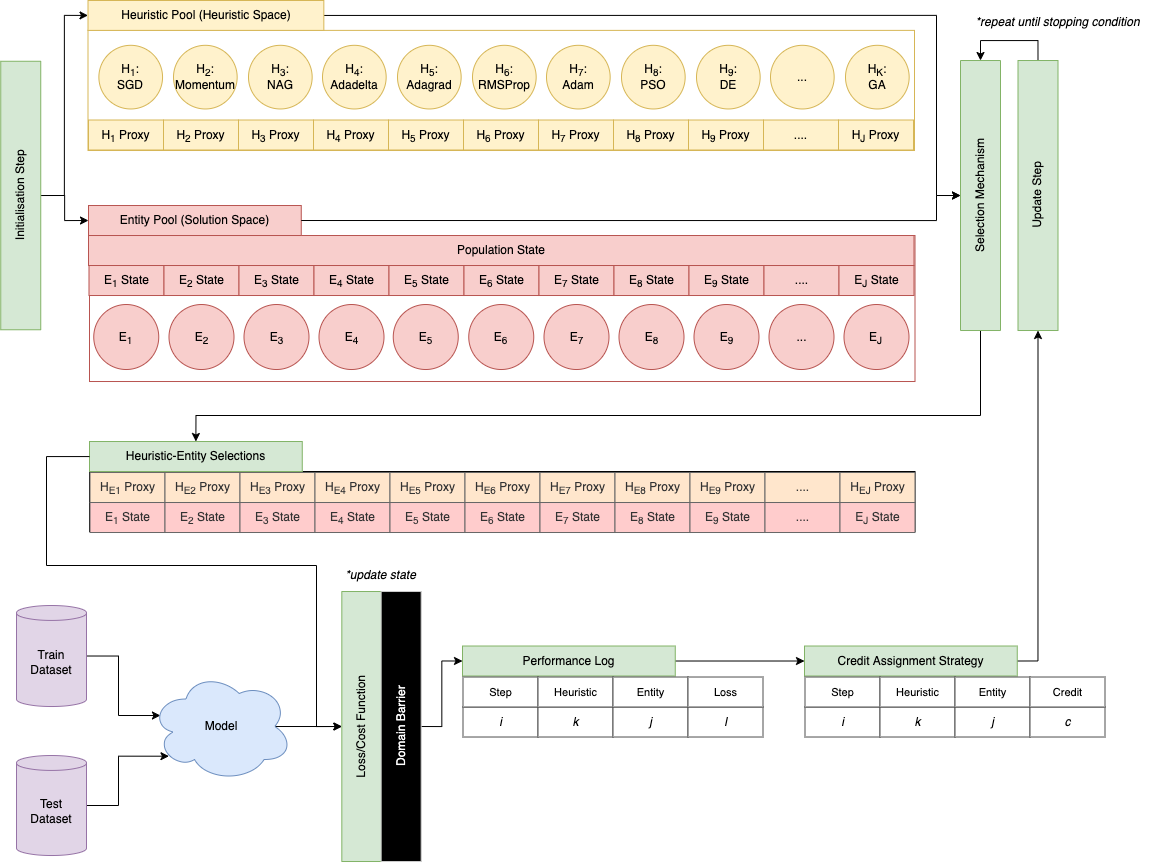
\includegraphics[width=1.0\textwidth]{bhh_architecture.png}
      \caption[The \index{Bayesian Hyper-Heuristics}Bayesian Hyper-Heuristic Architecture]{An illustration of
            the architecture and high level components of the \index{Bayesian Hyper-Heuristics}Bayesian Hyper-Heuristic.}
      \label{fig:bhh_architecture}
\end{figure}

At a high level, the architecture presented in Figure \ref{fig:bhh_architecture} above, presents the following main components:

\begin{itemize}
      \item \textbf{Heuristic Pool}: Contains a collection of low-level \index{heuristic}heuristics/\index{optimiser}optimisers. This is the \index{heuristic space}\textit{heuristic} space. Each heuristic has a proxy that is used to relay heuristic state update operations.

      \item \textbf{Entity Pool}: A collection of \index{entity}entities in a \index{population}population. These entities represent candidate solutions to the model. Each entity has its own state, but there is also a shared global population state.

      \item \textbf{Initialisation Step}: This is the execution of some initialisation strategy that determines how the entities in the entity pool (population) and the heuristics in the heuristic pool are initialised.

      \item \textbf{Selection Mechanism}: This is the implementation of the selection mechanism of selection \acp{HH}. In the case of the \ac{BHH}, the selection mechanism is a Bayesian probabilistic model.

      \item \textbf{Heuristic-Entity Selections}: This is the results of the selection mechanism. Heuristics are sampled/selected for each entity. Each entity's state will thus be manipulated by that particular heuristic's proxy methods.

      \item \textbf{Model}: The \index{model}model to be optimised. This forms the problem domain. In the case of this dissertation, the model is a \ac{FFNN}.Technically the model here simply refers to the architectural structure of the model, while entities represent that candidate solution (weights) to the model.

      \item \textbf{Train and Test Datasets}: The training set is used to train the model while the test set is used to evaluate the model's generalisation capabilities.

      \item \textbf{Loss/Cost Function}: The loss/cost function is the metric  by which the model is evaluated. In the case of supervised learning, the loss/cost function is a measure of distance between predicted output and the ground truth.

      \item \textbf{Domain Barrier}: A constraint on information flow, prohibiting high level components in the \index{heuristic space}\textit{heuristic} space from interacting and relaying information related to the \index{solution space}\textit{solution} space.

      \item \textbf{Performance Log}: Contains a record of heuristic-entity performance at each step of the training process.

      \item \textbf{Credit Assignment Strategy}: Implements a specific strategy to determine if the performance of an entity-heuristic combination is better than others or not.

      \item \textbf{Update Step}: The high level heuristic update step. This involves the mechanism by with the \ac{BHH} is optimised.
\end{itemize}

The above components are not described in enough detailed to properly illustrate their role in the \Ac{BHH}. To ensure proper clarity is given to each of these elements, a detailed discussion on each of these elements are presented next.


\index{Heuristic Pool}
\section{Heuristic Pool}
\label{sec:bhh:heuristic_pool}

This section discusses the concept of the heuristic pool, as implemented by the \ac{BHH}. Generally speaking, they heuristic pool is just a collection of low-level heuristics and make up the set of possible heuristics to select from. This is referred to as \text{heuristic space}. Importantly, since \acp{HH} optimise in heuristic space, it is from these lower-level heuristics that the \ac{BHH} must select and apply. The heuristic pool can then be defined in terms of size and/or heuristics that are included in the pool. These two aspects pose very important design choices. Both of these concepts can be empirically tested, however, one could argue the choice of design. Fundamentally, these design choices are about diversity. A brief discussion is given next on the trade-offs between exploration, exploitation and capability.

\index{Exploration}
\index{Exploitation}
\subsection{Diversity: Exploration, Exploitation and Capability}
\label{sec:bhh:heuristic_pool:diversity}

As with all \acp{HH}, the heuristics to be included in the heuristic pool is of great importance and should be carefully decided upon. A heuristic's eligibility for inclusion is determined by the following factors:

\begin{itemize}
      \item \textbf{Capability}: Certain heuristics are only capable of solving or optimising for certain problem types and domains. Examples include continuous vs. discrete, differentiable vs.  non-differentiable or static vs. dynamic problems.

      \item \textbf{Exploration and Exploitation Trade-off}: Some heuristics explore or exploit more than others. This could be due to the nature of the implementation or due to some hyper-parameter such as a learning rate.
\end{itemize}

An argument for diversity must thus be made. One of the benefits of \acp{HH} in general is that it will learn which heuristics to apply and when. The trade-off between exploration and exploitation should thus be outsourced to the \ac{BHH} itself. By including a diverse set of heuristics, based on the criteria mentioned above, the \ac{BHH} will learn to select and apply the appropriate heuristic at the appropriate time throughout the training process, naturally balancing a trade-off between exploration and exploitation. Heuristics that initially explore a lot should be selected when exploration is needed and heuristics that exploit a lot should be selected accordingly.

Notice however that diversity can not be achieved by simply including many different heuristics. The \ac{BHH} is still constraint by heuristic pool size. Consider that for every heuristic that is included, the demand for samples size required to learn with statistical certainty exponentially increases. Not only does a large heuristic pool drastically complicate the learning that is required by the \ac{BHH}, but it also drastically complicates the process of maintaining state. The next section provides the concept of heuristic update step proxies, an important component of the \ac{BHH}.

\index{Proxies}
\subsection{Proxies}
\label{sec:bhh:heuristic:proxies}

The concept of proxies arise from the sparsity of state as maintained by different heuristics. Since heuristics maintain different states, there is an uncertainty of state transition when switching between heuristics. Consider an example where the heuristic pool consists of just two heuristics. One heuristic is a gradient-based heuristic that maintains momentum such as \ac{Adam}. The other is a meta-heuristic that does not require a gradient at all such as \ac{PSO}. Both these heuristics track different parameters in their state. For \ac{Adam}, the expected gradient mean and variance is maintained, while the \ac{PSO} maintains record of the gbest and pbest solutions all of entities. A solution to this is to proxy heuristic state update operations. This allows us to maintain state in two parts:

\begin{itemize}
      \item \textbf{Primary State}: This refers to state the is originally maintained by a heuristic. The selected heuristic simply applies the normal state update operations to its state.

      \item \textbf{Proxied State}: This refers to state that is not directly maintained by the current selected heuristic, but can be updated by outsourcing the required state update operation to another heuristic.
\end{itemize}

Effectively this means that both primary and proxied state elements must be maintained together. Since entities represent candidate solutions, which are a form of state, entities are ideal components to store these state parameters. Thus, entities are extended to include the primary state elements of all the underlying low-level heuristics as well as the candidate solution (weights) for the model. At each heuristic-entity application step, all state elements per entity are updated either by primary method or by proxied method. The \ac{BHH} thus incorporates a state update operation proxy mapping as given in the example in Table \ref{tab:bhh:heuristic_pool:proxy_mapping_example} below.

\begin{table}[htbp]
      \centering
      \caption{State update operation proxy mapping example.}
      \label{tab:bhh:heuristic_pool:proxy_mapping_example}%
      \par\bigskip
      \resizebox{0.5\textwidth}{!}{
            \begin{tabular}{ccccc}
                                                                  &   & \multicolumn{3}{c}{State Parameter}                                                                                                                                                                                      \\
                  \cmidrule{3-5}                                  &   & 1                                                                      & 2                                                                      & 3                                                                      \\
                  \cmidrule{3-5}    \multirow{3}[1]{*}{Heuristic} & A & \cellcolor[rgb]{ .776,  .937,  .808}\textcolor[rgb]{ 0,  .38,  0}{n/a} & \cellcolor[rgb]{ 1,  .922,  .612}\textcolor[rgb]{ .612,  .341,  0}{B}  & \cellcolor[rgb]{ .776,  .937,  .808}\textcolor[rgb]{ 0,  .38,  0}{n/a} \\
                                                                  & B & \cellcolor[rgb]{ .776,  .937,  .808}\textcolor[rgb]{ 0,  .38,  0}{n/a} & \cellcolor[rgb]{ .776,  .937,  .808}\textcolor[rgb]{ 0,  .38,  0}{n/a} & \cellcolor[rgb]{ 1,  .922,  .612}\textcolor[rgb]{ .612,  .341,  0}{A}  \\
                                                                  & C & \cellcolor[rgb]{ .776,  .937,  .808}\textcolor[rgb]{ 0,  .38,  0}{n/a} & \cellcolor[rgb]{ 1,  .922,  .612}\textcolor[rgb]{ .612,  .341,  0}{B}  & \cellcolor[rgb]{ 1,  .922,  .612}\textcolor[rgb]{ .612,  .341,  0}{A}  \\
            \end{tabular}%
      }
\end{table}%

From the example given in Table \ref{tab:bhh:heuristic_pool:proxy_mapping_example}, when heuristic A is selected, it will outsource state update operations from heuristic B, for state parameter 2. Heuristic B will outsource from heuristic A, for state parameter 3. Finally, heuristic C will outsource from heuristic A and B, for state parameters 2 and 3 respectively. In this way, all heuristics maintain all the state parameters.

Notice however that this is a simple concept in principle, but requires detailed decomposition of the heuristics included in the heuristic pool.  Overlapping and unique state parameters must be identified so that a proxy mapping such as the one given in Table \ref{tab:bhh:heuristic_pool:proxy_mapping_example} can be constructed. A suggestion to simplify this process is to borrow concepts from the equations of motion from physics. These include \textit{position}, \textit{velocity}, \textit{acceleration} and \textit{momentum}. Expressing heuristic update steps according to these parameters drastically simplify the process. However, it is possible that heuristics implement unique state parameters that do not overlap, these have to be catered for in the proxy mapping.

These state parameters and update operations should not be considered in isolation. An example of this is position and velocity. Consider for example heuristics such as \acl{DE} and \aclp{GA}. These heuristics recombine entities. In this case, the concept of an equation of motion does not entirely make sense, since the displacement of its position is not a result of maintaining velocity or momentum, but rather by pure displacement through recombination. In this particular case, a solution to this is to apply the recombination operation to all secondary state parameters as well or to nullify secondary state parameters. Unfortunately there is no general solution and each heuristic must be carefully considered. The \ac{BHH} incorporates both of these approaches. The next section provides the reader with details around the entity pool.

\index{Entity Pool}
\section{Entity Pool}
\label{sec:bhh:entity_pool}

This section presents the details around the \index{entity pool}\textit{entity pool}. The \index{entity pool}entity pool refers to a collection of so-called individual \index{entity}\textit{entities}. A common naming convention for such a collection is a \textit{population} of entities. Similar to the heuristic pool that was described in Section \ref{sec:bhh:heuristic_pool} above, the entity pool size is an important design choice. The correct population size is thus a hyper-parameter that can be empirically evaluated.

The entity pool maintains two different types of state. These include entity (local) and population (global) state. Each of these are discussed in more detail next.

\index{Entity State}
\subsection{Entity State}
\label{sec:bhh:entity_pool:entity_state}

\index{entity}Entities represent \index{candidate solution}candidate solutions to the \index{model}model's trainable parameters (weights) and other heuristic-specific state parameters as was just discussed above in Section \ref{sec:bhh:heuristic:proxies}. It can be said that entities implement \textit{local} state. It was mentioned that these \index{entity}entities can be treated as physical \index{particle}\textit{particles} in a hyper-dimensional physical environment. This means that these \index{entity}entities model concepts from physics. For example, the candidate solution is represented as the \index{entity}entity's \textit{position} and an \index{entity}entity's velocity and acceleration, is analogous to the gradient and momentum of an \index{entity}entity respectfully. Examples of \index{Entity State}entity state parameters as derived from various low-level heuristics is given as follows:

\begin{itemize}
      \item \textbf{position}: General parameter that represents the actual candidate solution and is thus a primary state parameter for all heuristics.

      \item \textbf{velocity}: Directly implemented by heuristics such as \acp{PSO} can be derived proportionally from the gradient for gradient-based heuristics such as \ac{Momentum}.

      \item \textbf{gradient}: The last know gradient as derived from gradient-based heuristics.

      \item \textbf{position delta}: The last computed position delta between the current timestep and the previous timestep.

      \item \textbf{sum of the gradients squared}: As required and maintained by heuristics such as \ac{Adagrad}.

      \item \textbf{expected position delta variance}: As required and maintained by heuristics such as \ac{Adadelta}.

      \item \textbf{expected gradient mean}: As required and maintained by heuristics such as \ac{Momentum}, \ac{NAG} and \ac{Adam}.

      \item \textbf{expected gradient variance}: As required and maintained by heuristics such as \ac{RMSProp}, \ac{Adadelta} and \ac{Adam}.

      \item \textbf{personal best position}: Parameter that tracks that best known position by the entity thus far. As required and maintained by heuristics such as \ac{PSO}.

      \item \textbf{personal best loss}: Parameter that tracks that best known loss by the entity thus far. As required and maintained by heuristics such as \ac{PSO}.

      \item \textbf{loss}: General parameter that tracks the loss as achieved by the the entity throughout training.
\end{itemize}

From the list above it should become clear that entity state becomes increasingly complicated as the number of distinct heuristics included in the heuristic pool increases. Consider next the global state that is maintained.

\index{Population State}
\subsection{Population State}
\label{sec:bhh:entity_pool:population_state}


The \index{Population State}\textit{population state} refers to a collection of parameters that are shared between the \index{entity}entities in the population. This state is also referred to as \index{global state}\textit{global} state and represents the entity pool's memory of the population. The \index{population state}population state generally contains state parameters that are of importance to multiple heuristics and usually track the state of the population as a whole and not individual heuristic states. Some examples of population state that can arise from different heuristics is given below:

\begin{itemize}
      \item \textbf{\textit{entities}}: Naturally, the population state contains the list of entities in the population. List size determined by \index{Population Size}population size. Naturally this list contains multiple entities as with population based approaches such as \acp{PSO} and \acp{GA}.

      \item \textbf{\textit{ibest}} and \textbf{\textit{ibest loss}}: Refers to the best position and loss achieved by the population for the current iteration/step. This parameter is introduced by the \ac{BHH} itself through the requirements of the \textit{ibest} credit assignment strategy.

      \item \textbf{\textit{rbest}} and \textbf{\textit{rbest loss}}: Refers to the best position and loss achieved by the population for the current replay buffer/window size. This parameter is introduced by the \ac{BHH} itself through the requirements of the \textit{rbest} credit assignment strategy.

      \item \textbf{\textit{gbest}} and \textbf{\textit{gbest loss}}: Refers to the overall/global best position and loss achieved by the population for the entire training process. This parameter is introduced by heuristics such as \acp{PSO} and is also introduced by the \ac{BHH} itself through the requirements of the \textit{gbest} credit assignment strategy.
\end{itemize}

The reader was now introduced to both the heuristic pool and entity pool. The next section considers how the \ac{BHH} is initialised and makes specific reference to how these two pools of elements are initialised.

\section{Heuristic-Entity Selections}
\label{sec:bhh:heuristic_entity_selections}

The \ac{BHH} selects from the heuristic pool a low-level heuristic to be applied to an entity. The outcome of this selection process is a table that tracks which heuristic has been selected for which entity. The selection process is executed by the selection mechanism of the \ac{BHH} and is discussed later in Section \ref{sec:bhh:selection_mechanism}. These heuristic-entity combinations are applied to an underlying model. The next section provides clarity on the model component from the architecture of the \ac{BHH}.

\index{Model}
\section{Model}
\label{sec:bhh:model}

The \index{Model}model refers to the target \index{model}model to be optimised and is usually expressed as a complex mathematical function. For this dissertation, the authors focused specifically on shallow \acp{FFNN} (only one hidden layer). Figure \ref{fig:shallow_ffnn} below presents such a shallow \acp{FFNN}.

\begin{figure}[H]
      \centering
      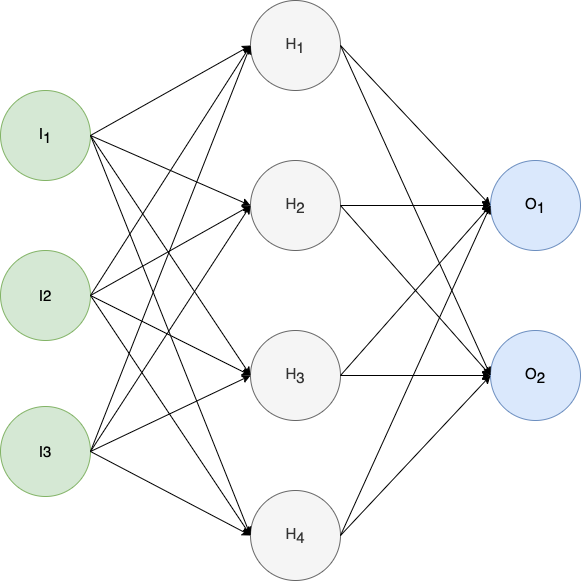
\includegraphics[width=0.4\textwidth]{shallow_ffnn.pdf}
      \caption[Shallow \index{Feedforward Neural Network}Feedforward Neural Network]{An illustration of
            a shallow \index{Feedforward Neural Network}Feedforward Neural Network.}
      \label{fig:shallow_ffnn}
\end{figure}

\section{Train and Test Datasets}
\label{sec:bhh:train_test_datasets}

The training of \ac{FFNN} is a supervised learning problem as was highlighted in Chapter \ref{chap:anns}. Therefore, the \ac{BHH} trains the model on training data from the training set, while is reserves an unseen set of test data in the test dataset for evaluation. It should be mentioned that the goal of the \ac{BHH} is to generalise well to the test set across a number of problem domains. As was previously mentioned, the test set should be sufficiently large to truly evaluate for generalisation capabilities. For the \ac{BHH}, it is proposed to have a 80-20\% split between the training and test set.

\section{Loss/Cost Function}
\label{sec:bhh:loss_function}

Chapter \ref{chap:anns} presented the concept of a loss/cost function that is used to evaluate the performance of \acp{ANN}. The \ac{BHH} uses this loss/cost function to evaluate the performance of a heuristic-entity combination. For classification problems, generally some entropy loss is used. For classification problems with 2 classes, \ac{BinXE} is used and for classification problems with more than 2 classes, the \ac{SparseCatXE} is used. For regression problems it is recommended to use some mean error measurement such as \ac{MSE} or \ac{RMSE}.

The loss/cost function is very important as this metric is used to evaluate model performance as a result of the application of a heuristic to an entity's candidate solution. The \ac{BHH} used this performance metric to bias towards good heuristic-entity combinations.  The continuous valued cost/loss function is translated into a discrete valued representation through a credit assignment strategy that is implemented in the \ac{BHH}. The credit assignment strategies is discussed in Section \ref{sec:bhh:credit_assignment_strategy}.

\section{Domain Barrier}
\label{sec:bhh:domain_barrier}

The domain barrier presents the boundary of information flow between the heuristic space and the solution space. It is mentioned in Section \ref{sec:bhh:loss_function} that the heuristic-entity loss is used by the \ac{BHH}. Notice that the \ac{BHH} uses this performance information and no information from the solution space itself. Furthermore, the \ac{BHH} maps this loss to a credit assignment problem as is mentioned by Burke et al.~\cite{ref:burke:2010}. The \ac{BHH} at a high level, is not aware of the actual candidate solution that is represented by the entity, but rather just that there is a candidate solution with a unique identifier that, together with a heuristic, produced a certain level of performance. The domain barrier is a feature that occurs in al \acp{HH}.  Burke et al.~\cite{ref:burke:2010} states that the \ac{HH} collects domain-independent information from the domain barrier. A number of examples of domain independent information is given, these include the number of heuristics, the changes in evaluation function, whether a new solution was found or generated, the distance between two solutions, whether it has become stuck.

\index{Performance Log}
\section{Performance Log}
\label{sec:bhh:performance_log}

Recall that the \ac{BHH} incorporates a Bayesian probabilistic implementation. Evidence is required to train the \ac{BHH}. The performance log is used to keep memory of a slice of the performance history. The performance log is simply a tabular implementation that tracks random events. The \ac{BHH} suggests the following metrics to keep track of in the performance log:

\begin{itemize}
      \item \textbf{step}: The current mini-batch step.

      \item \textbf{heuristic}: The selected heuristics' index.

      \item \textbf{entity}: The applied entity's index.

      \item \textbf{loss}: The heuristic-entity performance metric.

      \item \textbf{ibest loss}: Keeps track of the \textit{iteration} best loss. Thus, the best loss value achieved by all all entity-heuristic combinations for a single mini-batch step.

      \item \textbf{rbest loss}:  Keeps track of the \textit{replay} best loss. Thus, the best loss value achieved by all all entity-heuristic combinations over all mini-batch steps currently in the performance log.

      \item \textbf{gbest loss}:  Keeps track of the \textit{global} best loss. Thus, the best loss value achieved by all all entity-heuristic combinations over all mini-batch steps thus far.
\end{itemize}

The performance log as implemented by the \ac{BHH} is given in Table \ref{tab:bhh:performance_log:performance_log_example} below.

\begin{table}[htbp]
      \centering
      \caption{Performance log example showing the first 5 entity's selected heuristics for step 1 and their resulting performance measurements.}
      \label{tab:bhh:performance_log:performance_log_example}%
      \par\bigskip
      \resizebox{\textwidth}{!}{
            \begin{tabular}{cccccccc}
                  \textbf{step} & \textbf{entity} & \textbf{heuristic} & \textbf{loss} & \textbf{ibest loss} & \textbf{pbest Loss} & \textbf{rbest loss} & \textbf{gbest loss} \\
                  \midrule
                  1             & 1               & 1                  & 0.016444      & 0.016444            & 0.016444            & 0.016444            & 0.016444            \\
                  1             & 2               & 2                  & 0.337965      & 0.016444            & 0.337965            & 0.016444            & 0.016444            \\
                  1             & 3               & 1                  & 0.134781      & 0.016444            & 0.134781            & 0.016444            & 0.016444            \\
                  1             & 4               & 1                  & 0.998719      & 0.016444            & 0.998719            & 0.016444            & 0.016444            \\
                  1             & 5               & 3                  & 0.708702      & 0.016444            & 0.708702            & 0.016444            & 0.016444            \\
            \end{tabular}%
      }
\end{table}%

The performance log itself introduces a number of design considerations as well. Since the log contains a slice of memory, there should exists a trade-off between the following parameters:

\begin{itemize}
      \item \textbf{performance log size}: The larger the performance log, the longer memory is retained.The performance log size controls the recency of evidence from which new beliefs must be derived. This parameter is called the \textit{replay} window size, a term borrowed from \ac{RL} and should be empirically tested. If the replay window size is too small, it does not accumulate enough samples/evidence to really statistically make accurate classifications. If the replay window size is too back, the \ac{BHH} might remember too much of past performance and it could be that past performance is not indicative of future performance during the training process. Notice then that the performance log must be pruned to maintain a fixed replay window size. Dynamic replay window sizes is left as a research component for the future.

      \item \textbf{performance log reanalysis}: Consider the temporal nature of the performance log. Since it tracks all random events across all steps in the training process, it is needed to reanalyse the performance log appropriately in order to update the past information in the performance log with newly added data. An example of this is when a new rbest value has been found. Then the entire performance log's rbest loss must be updated.
\end{itemize}

The performance log should be considered along with the selection of credit assignment strategy used. These are discussed next.


\index{Credit Assignment Strategy}
\section{Credit Assignment Strategy}
\label{sec:bhh:credit_assignment_strategy}

The credit assignment strategy is an implementation that maps a continuous performance metric into a discrete credit metric. This component implements the ``move acceptance'' process as proposed by Özcan et al.~\cite{ref:ozcan:2006,ref:ozcan:2008}. It determines if a given performance is deemed good or not. This simple discrete transformation is subject to the credit assignment problem as discussed by Burke et al.~\cite{ref:burke:2010}. A good credit assignment strategy will correctly allocate credit to the appropriate heuristic-entity combination. THe magnitude of this credit is to be empirically tested.  It is later shown how these credit metrics are used to accumulate ``pseudo counts'' which concentrates/biases heuristic selection towards good performing heuristics. The \ac{BHH} propose the following initial credit assignment strategies.

\begin{itemize}
      \item \textbf{ibest}: Credit is assigned to the heuristic-entity combination that set the \textit{ibest} loss value, meaning that it is the entity-heuristic combination that achieved the best performance in the current mini-batch iteration.

      \item \textbf{pbest}: Credit is assigned to the heuristic-entity combination that set the \textit{pbest} loss value, meaning that it is the entity-heuristic combination that was able to improve on it's personal best past performance loss.

      \item \textbf{rbest}: Credit is assigned to the heuristic-entity combination that set the \textit{rbest} loss value, meaning that it is the entity-heuristic combination that achieved the best performance in the current replay window.

      \item \textbf{gbest}: Credit is assigned to the heuristic-entity combination that set the \textit{gbest} loss value, meaning that it is the entity-heuristic combination that achieved the overall best performance so far.

      \item \textbf{symmetric}: A credit assignment strategy that gives credit to all entity-heuristic combinations regardless of performance. This credit assignment strategy suggests that ``symmetric'' credit assignment be given. As a result, any bias that arise from uncertainty or as a result of an untrained \ac{BHH} model, in the beginning, is maintained and further strengthened throughout the training process . Notice that this credit assignment strategy does not randomly assign credit, it simply assigns credit to the all events that are a result of random selection, which could be possibly be biased.
\end{itemize}

The implementation of a credit assignment strategy is a pure, stateless function that translates input $P$ from the performance log into output $C$ as is given in Table \ref{tab:bhh:credit_assignment_strategy:credit_assignment_example} below.


\begin{table}[htbp]
      \centering
      \caption{Credit assignment strategy output table showing \textit{ibest} credit assignment for the first 5 entity's and their selected heuristics for step 1 of the training process.}
      \label{tab:bhh:credit_assignment_strategy:credit_assignment_example}%
      \par\bigskip
      \resizebox{0.4\textwidth}{!}{
            \begin{tabular}{cccc}
                  \textbf{step} & \textbf{entity} & \textbf{heuristic} & \textbf{credit} \\
                  \midrule
                  1             & 1               & 1                  & true            \\
                  1             & 2               & 2                  & false           \\
                  1             & 3               & 1                  & false           \\
                  1             & 4               & 1                  & false           \\
                  1             & 5               & 3                  & false           \\
            \end{tabular}%
      }
\end{table}%

Credit assignment is a key component of the \ac{BHH} is it will later be shown in Section \ref{sec:bhh:optimisation_step} how these credit assignments are used to optimise the \ac{BHH}. First, it is necessary to present the selection mechanism.


\index{Selection Mechanism}
\section{Selection Mechanism}
\label{sec:bhh:selection_mechanism}

This section aims to provide the reader with the detail around the selection mechanism as it is implemented by the \ac{BHH}. It is mentioned throughout this document that the \ac{BHH} implements a predictive model based on Bayesian probabilistic concepts. In probabilistic modeling it is necessary to identify all the random events that can occur.

\index{Random Events}
\subsection{Random Events}
\label{sec:bhh:selection_mechanism:random_events}

Observation of random events is treated as evidence. In the context of a Bayesian approach, this evidence is used to update prior beliefs. The \ac{BHH} distinguishes between the following events:

\begin{itemize}
      \item \textbf{$H$}: The event of observing \textit{heuristics}.
      \item \textbf{$E$}: The event of observing \textit{entities}.
      \item \textbf{$C$}: The event of observing \textit{credit assignments}.
\end{itemize}

It should be noted that this information is observed direclty from the performance log presented in Table \ref{tab:bhh:credit_assignment_strategy:credit_assignment_example} above. From the above list, the event $C$ is dependent on the occurrence of $H$ and $E$. However, for simplification, an argument for independence can be made.

\index{Independence}
\subsection{Independence}
\label{sec:bhh:selection_mechanism:independence}

The dependence between random events can have a drastic impact on the probabilistic model that is implemented. For simplicity, the \ac{BHH} assumes independence between events, although the event $C$ is clearly dependent on the occurrence of $H$ and $E$. Notice that the \ac{BHH} is fundamentally a classifier, classifying which heuristic to select given an entity and performance criteria. It is later shown in Section \ref{sec:bhh:selection_mechanism:naive_bayes} that the \ac{BHH} implements a Naïve Bayes classifier. Domingos et al.~\cite{ref:domingos:1997} mentions that although Bayesian classifiers’ probability estimates are only optimal under quadratic loss if the independence assumption holds, the classifier itself can be optimal under zero-one loss (misclassification rate) even when this assumption is violated by a wide margin. This means that independence can be assumed when the probabilistic model is used as a classifier and not to get real probabilities. Evaluating for proportionality and not precision allows for the assumption of independence.

\index{Bayes' Theorem}
\subsection{Bayes' Theorem}
\label{sec:bhh:selection_mechanism:bayes_theorem}

Section \ref{sec:bhh:selection_mechanism:random_events} presented the reader with the random events that are observed by the \ac{BHH} and Section \ref{sec:bhh:selection_mechanism:independence} provided an argument for independence between events. Chapter \ref{chap:probability} presented Bayes Theorem, but for convenience, it is given again in Equation~\eqref{eq:bhh:selection_mechanism:bayes_theorem} below.

\begin{equation}
      \label{eq:bhh:selection_mechanism:bayes_theorem}
      P(A \vert B) = \frac{P(B \vert A)P(A)}{P(B)}
\end{equation}

As was indicated in Section \ref{sec:bhh:selection_mechanism:independence}, Equation~\eqref{eq:bhh:selection_mechanism:bayes_theorem} can be evaluated for proportionality since the \ac{BHH} is not concerned with actual accurate selection probabilities, but rather implements a Bayesian classifier. The resulting proportionality is expressed in Equation~\eqref{eq:bhh:selection_mechanism:bayes_theorem_prop_to} below

\begin{equation}
      \label{eq:bhh:selection_mechanism:bayes_theorem_prop_to}
      P(A \vert B) \propto P(B \vert A)P(A)
\end{equation}

Notice how the Equation~\eqref{eq:bhh:selection_mechanism:bayes_theorem_prop_to} implements a Bayesian conditionally. This conditionality can be extended to include multiple criteria. The next section shows how the Bayesian classifier is implemented by providing the detail around the implemented predictive model.


\subsection{Predictive Model}
\label{sec:bhh:selection_mechanism:predictive_model}

Finally the reader is presented with the underlying predictive model as implemented by the \ac{BHH}. This component is arguably the most important component of the entire \ac{BHH} as it fundamentally drives the output of the \ac{BHH}. Bayes Theorem as was shown again in Section \ref{sec:bhh:selection_mechanism:bayes_theorem} above can be used to implement a predictive model to predict which heuristic to select, given the conditionality of a particular entity and a particular credit assignment criteria is met. Consider the following setup. Let

\begin{itemize}
      \item $I$: Denote the maximum number of instances in the replay window.
      \item $J$: Denote the entity pool (population) size.
      \item $K$: Denote the heuristic pool size.
      \item $L$: Denote the number of credit assignment output classes. Since the output of credit assignment is boolean, $L = 2$.

      \item $\alpha = (\alpha_{1}, \dots, \alpha_{K})$: Denote the concentration parameters for the heuristic probability distribution.
      \item $\beta = (\beta_{1}, \dots, \beta_{K})^{J}$: Denote the concentration parameters for the entity-heuristic probability distributions.
      \item $\gamma = (\gamma_{1}, \dots, \gamma_{K})^{L}$: Denote the concentration parameters for the credit-heuristic probability distribution.

      \item $\theta \vert \alpha \sim Dir(\alpha; K)$: Denote the heuristic probability distribution, implementing a Dirichlet probability distribution parameterised by $\alpha$ and $K$. Heuristic selection probabilities are sampled from this distribution.
      \item $\phi \vert \beta \sim Dir(\beta; K)^{J}$: Denote the entity-heuristic probability distribution, implementing a Dirichlet probability distribution parameterised by $\beta$ and $K$ for each entity in the entity pool with population size $J$. Entity-heuristic probabilities are sampled from this distribution.
      \item $\psi \vert \gamma_{1}, \gamma_{0}  \sim Beta(\gamma_{1}, \gamma_{0})$: Denote the credit-heuristic probability distribution, implementing a Beta probability distribution parameterised by $\gamma_{1}$ and $\gamma_{0}$. Credit-heuristic probabilities are sampled from this distribution.

      \item $H \vert \theta \sim Mult(\theta; I, K)$: Denote the distribution of heuristics (event $H$), implementing a Multinomial distribution, parameterised by the sampled heuristic selection probability $\theta$, the heuristic pool size $K$ and maximum number of instances $I$.
      \item $E \vert \phi \sim Mult(\phi; I, K)^{J}$: Denote the distribution of entity-heuristic combinations (event $E$), implementing a Multinomial distribution, parameterised by the sampled entity-heuristic selection probability $\phi$, the heuristic pool size $K$ and maximum number of instances $I$, for each entity in $J$.
      \item $C \vert \psi \sim Bin(\psi, I)$: Denote the distribution of credit-heuristic combinations (event $C$), implementing a Binomial distribution, parameterised by the sampled credit-heuristic selection probability $\psi$ and the maximum number of instances $I$.
\end{itemize}

The parameterised predictive model, as derived from Bayes theorem presented in Equation~\eqref{eq:bhh:selection_mechanism:bayes_theorem} is then given in Equation~\eqref{eq:bhh:selection_mechanism:predictive_model} below.

\begin{equation}
      \label{eq:bhh:selection_mechanism:predictive_model}
      \begin{split}
            P(H \vert E, C;  \theta, \phi, \psi)
            &= \frac{
                  P(E, C \vert H;  \phi, \psi)  P(H \vert \theta)
            }{
                  P(E, C \vert \theta, \phi, \psi)
            } \\
            &= \frac{
                  P(E \vert H;  \phi)  P(C \vert H;  \psi) P(H \vert \theta)
            }{
                  P(E \vert \theta, \psi) P(C \vert \theta, \phi)
            } \\
            &= \frac{
                  P(E \vert H;  \phi)  P(C \vert H;  \psi) P(H \vert \theta)
            }{
                  \left[ \sum_{k}^{K} P(E, H=k \vert \theta, \psi) \right] \left[ \sum_{k}^{K}  P(C, H=k \vert \theta, \phi) \right]
            } \\
            &= \frac{
                  P(E \vert H;  \phi)  P(C \vert H;  \psi) P(H \vert \theta)
            }{
                  \left[ \sum_{k}^{K} P(E \vert H=k \vert \phi) P(H=k \vert \theta) \right] \left[ \sum_{k}^{K} P(C \vert H=k \vert \psi) P(H=k \vert \theta) \right]
            }
      \end{split}
\end{equation}

Notice the joint probability over events $E$ and $C$ given the selection of a heuristic $H$ denoted by the sums of the products of the separate parts, for $E$ and $C$, in the denominator. The calculation in the denominator can be intractable as has been previously indicated. However, in order to derive the posterior distribution as given in Equation~\eqref{eq:bhh:selection_mechanism:bayes_theorem}), one only has to evaluate to proportionality as is given in Equation~\eqref{eq:bhh:selection_mechanism:predictive_model_prop_to} below.

\begin{equation}
      \label{eq:bhh:selection_mechanism:predictive_model_prop_to}
      \begin{split}
            P(H \vert E, C;  \theta, \phi, \psi) &\propto P(E \vert H;  \phi)  P(C \vert H;  \psi) P(H \vert \theta)
      \end{split}
\end{equation}

The predictive model thus models the \textit{proportional} probability of the event (selection of) heuristic $H$, given allocation to entity $E$ and credit $C$, parameterised by sampled $\theta$, $\phi$ and $\psi$. These parameters are in turn parameterised by concentrations $\alpha$, $\beta$, $\gamma_{1}$ and $\gamma_{0}$ which denote the prior beliefs of the \ac{BHH}.


\index{Naïve Bayes}
\subsection{Naïve Bayes}
\label{sec:bhh:selection_mechanism:naive_bayes}

This section aims to dissect the probabilistic model that is presented in Equestion \ref{eq:bhh:selection_mechanism:predictive_model_prop_to}. It has been established in Section \ref{sec:bhh:selection_mechanism:independence} that for \index{Naïve Bayes} naïve Bayes classifiers, independence between events can be assumed. The following derived \acp{PMF} are provided as fundamental building blocks that are later shown to be used in the optimisation process of the \ac{BHH} as is shown in Section \ref{sec:bhh:optimisation_step}.

The independence between events for the class label $H$ simply yields the \ac{PMF} of the Multinomial distribution as presented in Equation~\eqref{eq:bhh:selection_mechanism:naive_bayes:h_pmf} below.

\begin{equation}
      \label{eq:bhh:selection_mechanism:naive_bayes:h_pmf}
      \begin{split}
            P(H \vert \theta)
            &\propto \prod_{i=1}^{I} \prod_{k=1}^{K} P(h_{i,k} \vert \theta_{k}) \\
            &\propto \prod_{i=1}^{I} \prod_{k=1}^{K} \theta_{k}^{\mathbbm{1}_{1}(h_{i,k})} \\
            &\propto \prod_{k=1}^{K} \theta_{k}^{\sum_{i=1}^{I} \mathbbm{1}_{1}(h_{i,k})} \\
            &\propto \prod_{k=1}^{K} \theta_{k}^{N_{k}}
      \end{split}
\end{equation}

Where $N_{k}$ is a summary variable such that $N_{k} = \sum_{i=i}^{I}
      \mathbbm{1}_{1}(h_{i,k})$, denoting the count of occurrences of the event
$h_{i}$ taking on class $k$, i.e. the count of occurrences of heuristic $k$ in
$I$ independent, identical runs.

The independence between events $E$ given class label $H$ is denoted by the likelihood of $E$
conditional to the occurrence of heuristic $k$ and model parameter $\phi$ as
presented in Equation~\eqref{eq:bhh:selection_mechanism:naive_bayes:EgH_pmf} below.

\begin{equation}
      \label{eq:bhh:selection_mechanism:naive_bayes:EgH_pmf}
      \begin{split}
            P(E \vert H;  \phi)
            &\propto \prod_{i=1}^{I} \prod_{j=1}^{J} \prod_{k=1}^{K} P(e_{i,j,k} \vert h_{i,k} ; \phi_{j,k})  \\
            &\propto \prod_{i=1}^{I} \prod_{j=1}^{J} \prod_{k=1}^{K} \phi_{j,k}^{\mathbbm{1}_{1}(e_{i,j,k})\mathbbm{1}_{1}(h_{i,k})} \\
            &\propto \prod_{j=1}^{J} \prod_{k=1}^{K} \phi_{j,k}^{ \sum_{i}^{I} \left[ \mathbbm{1}_{1}(e_{i,j,k}) \mathbbm{1}_{1}(h_{i,k}) \right]} \\
            &\propto \prod_{j=1}^{J} \prod_{k=1}^{K} \phi_{j,k}^{N_{j,k}}
      \end{split}
\end{equation}

Where $N_{j,k}$ is a summary variable such that $N_{j,k} = \sum_{i=i}^{I}
      \mathbbm{1}_{1}(e_{i,j,k})\mathbbm{1}_{1}(h_{i,k})$, denoting the count of
occurrences of the events $e_{i}$ taking on class $j$ and $h_{i}$ taking on
class $k$, i.e. the count of occurrences of both entity entity $e$ and heuristic
$k$ occurring together in $I$ independent, identical runs.

Finally, the independence between events for the performance criteria feature $C$ given class
label $H$ is denoted by the likelihood of $C$ conditional to the occurrence of
heuristic $k$ and model parameter $\psi$ as given in Equation~\eqref{eq:bhh:selection_mechanism:naive_bayes:CgH_pmf} below.

\begin{equation}
      \label{eq:bhh:selection_mechanism:naive_bayes:CgH_pmf}
      \begin{split}
            P(C\vert H;  \psi)
            &\propto\prod_{i=1}^{I} \prod_{k=1}^{K} P(c_{i,k} \vert h_{i,k} ; \psi_{k})  \\
            &\propto \prod_{i=1}^{I} \prod_{k=1}^{K} \psi_{k}^{\mathbbm{1}_{1}(c_{i,k})\mathbbm{1}_{1}(h_{i,k})} (1 - \psi_{k})^{\mathbbm{1}_{0}(c_{i,k})\mathbbm{1}_{1}(h_{i,k})}\\
            &\propto \prod_{k=1}^{K} \psi_{k}^{\sum_{i=1}^{I} \mathbbm{1}_{1}(c_{i,k})\mathbbm{1}_{1}(h_{i,k})} (1 - \psi_{k})^{\sum_{i=1}^{I} \mathbbm{1}_{0}(c_{i,k})\mathbbm{1}_{1}(h_{i,k})}\\
            &\propto \prod_{k=1}^{K} \psi_{k}^{N_{1,k}} (1 - \psi_{k})^{N_{0,k}} \\
            &\propto \prod_{k=1}^{K} \psi_{k}^{N_{1,k}} (1 - \psi_{k})^{(N_{k} - N_{1,k})}
      \end{split}
\end{equation}

Where $N_{k}$ is the summary variable as described for Equation~\eqref{eq:bhh:selection_mechanism:naive_bayes:CgH_pmf} above.
$N_{1,k}$ is a summary variable such that $N_{1,k} = \sum_{i=1}^{I}
      \mathbbm{1}_{1}(c_{i,k})\mathbbm{1}_{1}(h_{i,k})$, denoting the count of
occurrences of the events $c_{i}$ taking on a success $(c_{i}=1)$ and $h_{i}$
taking on class $k$, i.e. the count of occurrences of both succeeding in the
performance criteria and heuristic $k$ occurring together in $I$ independent,
identical runs. Similarly $N_{0,k} = N_{k} - N_{1,k}$ would denote the count of
occurrences of the events $c_{i}$ taking on a failure $(c_{i}=0)$ and $h_{i}$
taking on class $k$.


Given the assumptions of the naïve Bayes classifier, one could supplement Equations \ref{eq:bhh:selection_mechanism:naive_bayes:h_pmf}, \ref{eq:bhh:selection_mechanism:naive_bayes:EgH_pmf} and \ref{eq:bhh:selection_mechanism:naive_bayes:CgH_pmf} above into the proportional evaluation of the predictive model as given in Equation~\eqref{eq:bhh:selection_mechanism:predictive_model_prop_to}. This is presented in Equation~\eqref{eq:bhh:selection_mechanism:naive_bayes:HgEC_pmf} below.

\begin{equation}
      \label{eq:bhh:selection_mechanism:naive_bayes:HgEC_pmf}
      \begin{split}
            P(H \vert E, C;  \theta, \phi, \psi)
            &\propto P(E \vert H;  \phi)  P(C \vert H;  \psi) P(H \vert \theta)  \\
            &\propto \left[ \prod_{j=1}^{J} \prod_{k=1}^{K} \phi_{j,k}^{N_{j,k}} \right] \left[ \prod_{k=1}^{K} \psi_{k}^{N_{1,k}} (1 - \psi_{k})^{(N_{k} - N_{1,k})} \right] \left[ \prod_{k=1}^{K} \theta_{k}^{N_{k}} \right]
      \end{split}
\end{equation}

Computationally the equation presented in Equation~\eqref{eq:bhh:selection_mechanism:naive_bayes:HgEC_pmf} will underflow if the resulting probabilities are very small.


\index{Numerical Stability}
\subsection{Numerical Stability}
\label{sec:bhh:selection_mechanism:numerical_stability}

When evaluating for Equation~\eqref{eq:bhh:selection_mechanism:naive_bayes:HgEC_pmf}, the numerical stability is shown to underflow if the resulting probabilities from its parts are very small. Multiplying multiple fractional parameters leads to an even smaller fractional number. Probabilities might be very low at some points during training. Consider an example where training has stagnated, effectively leading to a scenario where a credit assignment strategy never fulfills a credit assignment, yielding an extremely small probability for $\psi$. A solution to this problem is to apply the \textit{log-sum-exp trick}, parameterising distributions no longer using logits rather than probabilities. The transformation of Equation~\eqref{eq:bhh:selection_mechanism:naive_bayes:HgEC_pmf} using the log-sum-exp trick is given below in Equation~\eqref{eq:bhh:selection_mechanism:numerical_stability:log_sum_exp}.

\begin{equation}
      \label{eq:bhh:selection_mechanism:numerical_stability:log_sum_exp}
      \begin{split}
            LSE(P(h_{k} \vert e_{j}, c_{1};  \theta, \phi, \psi)) = \ln(\exp(\phi_{j,k}) +  \exp(\psi_{k}) + \exp(\theta_{k}))
      \end{split}
\end{equation}

The log-sum-exp trick as shown above caters for very small probabilities, however, there might be a situation where  a random event is never seen, purely by chance. This results in a scenario referred to as \textit{mode collapse} and is discussed next.

\index{Mode Collapse}
\subsection{Mode Collapse}
\label{sec:bhh:selection_mechanism:mode_collapse}

Mode collapse is the situation that occurs where the selective pressure towards a heuristic is close to zero, as a results of random sampling, low initial bias or bad performance. This leads to a situation where to probabilistic model continually decrease the selective pressure until the selection probability of that heuristic is 0, yielding no further observations of that particular random event. This could be problematic and should be addressed.

The \ac{BHH} addresses this issue by:

\begin{itemize}
      \item Using \textit{symmetric} initialisation of the concentration parameters $\alpha$, $\beta$, $\gamma_{1}$ and $\gamma_{0}$.

      \item Setting the lower-bound of the concentration parameters $\alpha$, $\beta$, $\gamma_{1}$ and $\gamma_{0}$ to 1, so that a selection probability of 0 is highly improbable.

      \item Continuously resampling heuristics throughout the training process, before and after optimisation, eliminating mode collapse as a result of just random sampling.
\end{itemize}

Another suggestion is to ensure that at least one of every heuristic is always selected during training. The \ac{BHH} does not incorporate this model as this could result in a situation where a bad choice of heuristic is continually used throughout the training process, possibly resulting in bad update steps/selections. Instead the \ac{BHH} relies on the underlying learning process to control the selective pressure according to performance and nothing else. If this leads to a situation where mode collapse occurs, the \ac{BHH} accepts this outcome.

This section briefly touched on parameter initialisation. The next section discusses the initialisation process of the \ac{BHH} in detail.

\section{Initialisation Step}
\label{sec:bhh:initialisation_step}

This section sheds light into the initialisation of the \ac{BHH} and how it applies to the heuristic and entity pools. Since the heuristic pool is a collection of stateless heuristic proxy operations, there is no explicit initialisation that is applied to the heuristic pool itself. On the contrary, the entity pool is stateful and maintain candidate solutions. Chapter \ref{chap:anns} presented various initialisation strategies to randomly place candidate solutions in the solution space. The \ac{BHH} can make use of any of these initialisation strategies and as such, by default makes use of \index{Glorot uniform sampling}Glorot uniform sampling. All other entity state parameters are initialised to be zero.

The selection mechanism also requires initialisation. Section \ref{sec:bhh:selection_mechanism:predictive_model} introduces the concentration parameters $\alpha$, $\beta$, $\gamma_{1}$ and $\gamma_{0}$. These parameters \textit{symmetrically} initialised, meaning that they are all initialised to the value of one in all dimensions. Section \ref{sec:bhh:optimisation_step:a_priori_bias} shows that these concentration parameters can be used to introduce \textit{a priori} biases based on expert knowledge. The next section provides the detail around the selection mechanism that is implemented by the \ac{BHH}.


\section{Optimisation Step}
\label{sec:bhh:optimisation_step}

Thus far the reader has been presented with all the fundamental components of the \ac{BHH}. The final step that is missing is to present the optimisation step by which the optimisation process takes place. This section aims to provide a solid  mathematical explanation to show exactly how the \ac{BHH} is able to learn.

The \ac{BHH} is an adaptive \ac{HH}, meaning that it implements online learning. Online learning refers to the continuous learning process that is executed by the \ac{BHH} while training is taking place. Throughout the training process, concentration parameters are updated strategically to guide the selection mechanism towards heuristics that perform well. The learning capability of the \ac{BHH} lies in the careful updating of these concentration parameters.

Generally there are two different techniques that are used to train naïve Bayes classifiers. The frequentist approach implements \ac{MLE} and the Bayesian approach implements \ac{MAP}. These methods are provided in Sections \ref{sec:bhh:optimisation_step:mle} and \ref{sec:bhh:optimisation_step:map} respectively. It should be mentioned that the \ac{BHH} makes use of \ac{MAP} to optimise the underlying model, however, the authors deem it necessary to provide the details of \ac{MLE} as it contains fundamental mathematical building blocks that are required to understand \ac{MAP}.

It has been established that the \ac{BHH} is a selective \ac{HH} that biases heuristic selection towards a certain performance bias. The concept of performance biases is discussed next.

\index{Performance Bias}
\subsection{Performance Bias}
\label{sec:bhh:optimisation_step:performance_bias}

The intent of the \ac{BHH} is to gather evidence that is can use to update its prior beliefs about which heuristics perform well during training. These beliefs are represented by the concentration parameters $\alpha$, $\beta$, $\gamma_{1}$ and $\gamma_{0}$. A change in prior beliefs is represented by a change in these concentration parameters. Sections \ref{sec:bhh:optimisation_step:mle} and \ref{sec:bhh:optimisation_step:map} show how the concentration parameters are updated throughout the training process, yielding the mechanism by which optimisation takes place.

Specifically, it can be said, that the optimisation process employed by the \ac{BHH} updates \textit{pseudo counts} of events that it observes in its performance logs. These pseudo counts track the occurrence of a heuristic, an entity and resulting performance of these two elements. Through the credit assignment strategy that was discussed in Section \ref{sec:bhh:credit_assignment_strategy}, these pseudo counts are biased towards entity-heuristic combinations that meet credit requirements and yield credit allocations i.e. credit pseudo counts. It is through this concept that the \ac{BHH} is able to bias selection towards performance.

The above mentioned concepts discuss heuristic selection bias by means of online learning. Another possibility is to introduce \textit{a priori} information in the form of expert knowledge. This concept is discussed next.

\index{A Priori Bias}
\subsection{A Priori Bias}
\label{sec:bhh:optimisation_step:a_priori_bias}

Section \ref{sec:bhh:optimisation_step:performance_bias} above discusses the role of concentration parameters on the \ac{BHH}. It is further mentioned in Section \ref{sec:bhh:initialisation_step} that these concentration parameters are symmetrically initialised. This simply means that they are uniformly initialised to all have the value of one in all dimensions.

Consider that the intent of the \ac{BHH} is to learn which heuristics to select during training. An expert can inject expert knowledge into the \ac{BHH} by means of these concentration parameters. An example of this is given as follows. It might be well known that a particular heuristic will perform well on a given problem domain. This could be through empirical analysis, part experiences, logical reasoning and deduction or simply by nature of the heuristic itself. A slight bias can be introduced to this heuristic before training starts but slightly scaling the initialised concentration parameter for that particular heuristic so that is more than the other concentration parameters. The \ac{BHH} interprets this encoded concentration parameter as a prior belief and aims to update this parameter as new evidence is collected. The next section introduces the mathematics behind \ac{MLE}.

\index{Maximum Likelihood Estimation}
\subsection{Maximum Likelihood Estimation}
\label{sec:bhh:optimisation_step:mle}

In probability theory and statistics, \ac{MLE} is a method that estimates the parameters of some assumed prior probability distribution given newly observed data and evidence. This section shows that the values for $\theta$, $\phi$ and $\psi$ can be estimated by \ac{MLE} to yield equations \ref{eq:bhh:optimisation_step:mle:theta}, \ref{eq:bhh:optimisation_step:mle:phi} and \ref{eq:bhh:optimisation_step:mle:psi} below.

\begin{equation}
      \label{eq:bhh:optimisation_step:mle:theta}
      \begin{split}
            \hat{\theta}_{k} = E[\theta_{k}] = \frac{N_{k}}{N}
      \end{split}
\end{equation}

\begin{equation}
      \label{eq:bhh:optimisation_step:mle:phi}
      \begin{split}
            \hat{\phi}_{j,k} = E[\phi_{j,k}] = \frac{N_{j,k}}{N_{j}}
      \end{split}
\end{equation}

\begin{equation}
      \label{eq:bhh:optimisation_step:mle:psi}
      \begin{split}
            \hat{\psi}_{k} = E[\psi_{k}] = \frac{N_{1,k}}{N_{k}}
      \end{split}
\end{equation}

The calculations of the \ac{MLE} for $\hat{\theta}_{k}$, $\hat{\phi}_{j,k}$ and
$\hat{\psi}_{k}$ are now presented. The log likelihood of $\hat{\theta}$, $\hat{\phi}$ and $\hat{\psi}$ as derived
from the Equation~\eqref{eq:bhh:selection_mechanism:predictive_model_prop_to} is given in Equation~\eqref{eq:bhh:optimisation_step:mle:log_likelihood_all} below.

\begin{equation}
      \label{eq:bhh:optimisation_step:mle:log_likelihood_all}
      \begin{split}
            & \mathcal{L}(\theta, \phi, \psi) \\
            &= \ln\left(\left[ \prod_{j=1}^{J} \prod_{k=1}^{K} \phi_{j,k}^{N_{j,k}} \right] \left[ \prod_{k=1}^{K} \psi_{k}^{N_{1,k}} (1 - \psi_{k})^{(N_{k} - N_{1,k})} \right] \left[ \prod_{k=1}^{K} \theta_{k}^{N_{k}} \right] \right) \\
            &= \ln \left( \prod_{j=1}^{J} \prod_{k=1}^{K} \phi_{j,k}^{N_{j,k}} \right) +  \ln \left( \prod_{k=1}^{K} \psi_{k}^{N_{1,k}} (1 - \psi_{k})^{(N_{k} - N_{1,k})} \right) + \ln \left( \prod_{k=1}^{K} \theta_{k}^{N_{k}} \right) \\
            &= \left( \sum_{j=1}^{J} \sum_{k=1}^{K} N_{j,k} \ ln \left( \phi_{j,k}
            \right) \right) \\
            &+ \left( \sum_{k=1}^{K} N_{1,k} \ln \left( \psi_{k} \right) + \left( N_{k} - N_{1,k} \right) \ln \left( 1 - \psi_{k} \right) \right) + \left( \sum_{k=1}^{K} N_{k} \ln \left( \theta_{k} \right) \right)
      \end{split}
\end{equation}

Equation~\eqref{eq:bhh:optimisation_step:mle:log_likelihood_all} can be broken down into each of its factors. Consider the log likelihood of $\psi$  as denoted by Equation~\eqref{eq:bhh:optimisation_step:mle:log_likelihood_psi} below.

\begin{equation}
      \label{eq:bhh:optimisation_step:mle:log_likelihood_psi}
      \begin{split}
            \mathcal{L}(\psi) &=  \sum_{k=1}^{K} N_{1,k} \ln \left( \psi_{k} \right) + \left( N_{k} - N_{1,k} \right) \ln \left( 1 - \psi_{k} \right)
      \end{split}
\end{equation}

The MLE for $\hat{\psi_{k}} $ can be calculated by taking the derivative of Equation~\eqref{eq:bhh:optimisation_step:mle:log_likelihood_psi} with respect to $\psi_{k}$ and equating to zero as presented in Equation~\eqref{eq:bhh:optimisation_step:mle:proof_log_likelihood_psi} as follows.

\begin{equation}
      \label{eq:bhh:optimisation_step:mle:proof_log_likelihood_psi}
      \begin{split}
            \frac{\partial \mathcal{L}(\psi)}{\partial \psi_{k}} &= N_{1,k} \frac{1}{ \psi_{k}} + \left( N_{k} - N_{1,k} \right) \frac{-1}{ \left( 1 - \psi_{k} \right) } \\
            0 &=  \frac{ N_{1,k} \left( 1 - \psi_{k} \right) +  \left( N_{1,k} - N_{k} \right) \psi_{k}}{ \psi_{k} \left( 1 - \psi_{k} \right) } \\
            0 &=  N_{1,k} \left( 1 - \psi_{k} \right) +  \left( N_{1,k} - N_{k} \right) \psi_{k} \\
            0 &=  N_{1,k} - N_{1,k} \psi_{k}  +  N_{1,k} \psi_{k} - N_{k}\psi_{k} \\
            0 &=  N_{1,k} - N_{k}\psi_{k} \\
            N_{k}\psi_{k} &=  N_{1,k} \\
            \hat{\psi}_{k} &=  \frac{N_{1,k}}{N_{k}} \\
      \end{split}
\end{equation}


The value for $\hat{\theta_{k}} $ can be calculated similarly. However, one has to compensate for the $K-1$ simplex $S$ by adding error factor $\epsilon$ to correct values for  $\theta$ where $\sum_{k}^{K} \theta_{k} \neq 1$. The new log likelihood function is then given in Equation~\eqref{eq:bhh:optimisation_step:mle:proof_log_likelihood_theta_part_1} below.

\begin{equation}
      \label{eq:bhh:optimisation_step:mle:proof_log_likelihood_theta_part_1}
      \begin{split}
            \mathcal{L}(\theta, \epsilon)
            &=  \left( \sum_{k=1}^{K} N_{k} \ln \left( \theta_{k} \right) \right) + \epsilon \left( 1 - \sum_{k=1}^{K} \theta_{k} \right) \\
            &=  \left( \sum_{k=1}^{K} N_{k} \ln \left( \theta_{k} \right) \right) + \left( \epsilon -  \epsilon \sum_{k=1}^{K} \theta_{k} \right)
      \end{split}
\end{equation}

Solving first for $\epsilon$ yields Equation~\eqref{eq:bhh:optimisation_step:mle:proof_log_likelihood_theta_part_2} below.

\begin{equation}
      \label{eq:bhh:optimisation_step:mle:proof_log_likelihood_theta_part_2}
      \begin{split}
            \frac{\partial \mathcal{L}(\theta, \epsilon)}{\partial \epsilon} &= 1 - \sum_{k=1}^{K} \theta_{k}  \\
            \sum_{k=1}^{K} \theta_{k}  &= 1
      \end{split}
\end{equation}

Then solving for $\theta_{k}$ yields Equation~\eqref{eq:bhh:optimisation_step:mle:proof_log_likelihood_theta_part_3} as presented below.

\begin{equation}
      \label{eq:bhh:optimisation_step:mle:proof_log_likelihood_theta_part_3}
      \begin{split}
            \frac{\partial \mathcal{L}(\theta, \epsilon)}{\partial \theta_{k}} &=  N_{k} \frac{1}{\theta_{k}}  + \epsilon(-1) \\
            \frac{N_{k}}{\theta_{k}} &= \epsilon \\
            N_{k} &= \theta_{k} \epsilon \\
            \sum_{k=1}^{K} N_{k} &= \sum_{k=1}^{K} \theta_{k} \epsilon \\
            N &= \epsilon \sum_{k=1}^{K} \theta_{k} \\
            N &= \epsilon
      \end{split}
\end{equation}

Substituting back into the Equation yields Equation~\eqref{eq:bhh:optimisation_step:mle:proof_log_likelihood_theta_part_4} below.

\begin{equation}
      \label{eq:bhh:optimisation_step:mle:proof_log_likelihood_theta_part_4}
      \begin{split}
            N_{k} &= \theta_{k} \epsilon \\
            N_{k} &= \theta_{k} N \\
            \hat{\theta}_{k} &= \frac{N_{k}}{N}\\
      \end{split}
\end{equation}

The value for $\hat{\phi}_{j, k} $ is calculated very similarly. To compensate for the $K-1$ simplex $S$ an error factor $\lambda = (\lambda_{1}, \dots, \lambda_{J})$ is added. This follows in Equation~\eqref{eq:bhh:optimisation_step:mle:proof_log_likelihood_phi_part_1} as is presented below.

\begin{equation}
      \label{eq:bhh:optimisation_step:mle:proof_log_likelihood_phi_part_1}
      \begin{split}
            \mathcal{L}(\phi, \lambda)
            &=  \left( \sum_{j=1}^{J} \sum_{k=1}^{K} N_{j,k} \ ln \left( \phi_{j,k} \right) \right) + \sum_{j=1}^{J} \lambda_{j} \left( 1 - \sum_{k=1}^{K} \phi_{j,k} \right) \\
            &=  \left( \sum_{j=1}^{J} \sum_{k=1}^{K} N_{j,k} \ ln \left( \phi_{j,k} \right) \right) + \sum_{j=1}^{J} \lambda_{j} - \sum_{j=1}^{J} \lambda_{j} \sum_{k=1}^{K} \phi_{j,k} \\
      \end{split}
\end{equation}

Solving first for $\lambda_{j}$ yields Equation~\eqref{eq:bhh:optimisation_step:mle:proof_log_likelihood_phi_part_2} as is given below.

\begin{equation}
      \label{eq:bhh:optimisation_step:mle:proof_log_likelihood_phi_part_2}
      \begin{split}
            \frac{\partial \mathcal{L}(\phi, \lambda)}{\partial \lambda_{j}} &= 1 - \sum_{k=1}^{K} \phi_{j,k}  \\
            \sum_{k=1}^{K} \phi_{j,k}  &= 1
      \end{split}
\end{equation}

Then solving for $\phi_{j,k}$ yields Equation~\eqref{eq:bhh:optimisation_step:mle:proof_log_likelihood_phi_part_3} below.

\begin{equation}
      \label{eq:bhh:optimisation_step:mle:proof_log_likelihood_phi_part_3}
      \begin{split}
            \frac{\partial \mathcal{L}(\phi, \lambda)}{\partial \phi_{j,k}} &= N_{j,k} \frac{1}{\phi_{j,k}}  - \lambda_{j} \\
            \frac{N_{j,k}}{\phi_{jk}} &= \lambda_{j} \\
            N_{j,k} &= \phi_{j,k} \lambda_{j} \\
            \sum_{k=1}^{K} N_{j,k} &= \sum_{k=1}^{K} \phi_{j,k} \lambda_{j} \\
            N_{j} &= \lambda_{j} \sum_{k=1}^{K} \phi_{j,k} \\
            N_{j} &= \lambda_{j}
      \end{split}
\end{equation}

Substituting back into the Equation yields equation \ref{eq:bhh:optimisation_step:mle:proof_log_likelihood_phi_part_4} below.

\begin{equation}
      \label{eq:bhh:optimisation_step:mle:proof_log_likelihood_phi_part_4}
      \begin{split}
            N_{j,k} &= \phi_{j,k} \lambda_{j} \\
            N_{j,k} &= \phi_{j,k} N_{j} \\
            \hat{\phi}_{j,k} &= \frac{N_{j,k}}{N_{j}}\\
      \end{split}
\end{equation}

This section provided the mathematical derivations of the MLE equations for $\theta$, $\phi$ and $\psi$. The next section provides the detail around \ac{MAP}, the optimisation process utilised by the \ac{BHH}.

\index{Maximum a Posteriori Estimation}
\subsection{Maximum a Posteriori Estimation}
\label{sec:bhh:optimisation_step:map}

Another approach to optimising the values for $\hat{\theta}_{k}$, $\hat{\phi}_{j,k}$ and $\hat{\psi}_{k}$ is to optimise the parameters by their probability distributions' parameters. This process is referred to as \index{Bayesian analysis}\textit{Bayesian analysis}. This section provides the mathematical details of the Bayesian analysis and \ac{MAP} as it is implemented by the \ac{BHH}.

Bayesian analysis makes use of the \textit{posterior} probability distribution. The posterior distribution is simply expressed as:

\begin{equation*}
      \label{eq:bhh:optimisation_step:map:bayesian_analysis_lamens}
      \begin{split}
            POSTERIOR \propto LIKELIHOOD \times PRIOR
      \end{split}
\end{equation*}

The likelihood is presented in Equation~\eqref{eq:bhh:optimisation_step:map:bayesian_analysis_lamens} above. The event $H$ is a multinomial distribution with parameter $\theta$. It is known that the conjugate prior to a multinomial distribution is a Dirichlet probability distribution (see Chapter \ref{chap:probability}. The \textit{prior} probability distribution for  $\theta_{k}$ is thus presented in Equation~\eqref{eq:bhh:optimisation_step:map:map_theta_prior} below.

\begin{equation}
      \label{eq:bhh:optimisation_step:map:map_theta_prior}
      \begin{split}
            P(\theta | \alpha)
            &\propto \prod_{k=1}^{K} \theta_{k}^{\alpha_{k} -1}
      \end{split}
\end{equation}

Furthermore, the event $E$ is also a multinomial distribution with parameter $\phi$. The \textit{prior} probability distribution for $\phi_{j,k}$ is thus presented in Equation~\eqref{eq:bhh:optimisation_step:map:map_phi_prior} below.

\begin{equation}
      \label{eq:bhh:optimisation_step:map:map_phi_prior}
      \begin{split}
            P(\phi \vert \beta)
            &\propto \prod_{j=1}^{J}  \prod_{k=1}^{K} \phi_{j,k}^{\beta_{j,k} -1}
      \end{split}
\end{equation}

Finally, the event $C$ is a binomial distribution with parameter $\psi$. It is known that the conjugate prior to a binomial distribution is a Beta probability distribution (see Chapter \ref{chap:probability}). The prior probability distribution for $\psi_{k}$ is thus presented in Equation~\eqref{eq:bhh:optimisation_step:map:map_psi_prior} below.

\begin{equation}
      \label{eq:bhh:optimisation_step:map:map_psi_prior}
      \begin{split}
            P(\psi | \gamma_{1}, \gamma_{0})
            &\propto \prod_{k=1}^{K} \psi_{k}^{\gamma_{1,k}} (1- \psi_{k})^{\gamma_{2,k}}
      \end{split}
\end{equation}

Putting the likelihood and priors together yields the posterior distribution as given in Equation~\eqref{eq:bhh:optimisation_step:map:map_psi_prior} below.

\begin{equation}
      \label{eq:bhh:optimisation_step:map:posterior}
      \begin{split}
            & P(\theta, \phi, \psi \vert H, E, C;  \alpha, \beta, \gamma_{1}, \gamma_{0}) \\
            &\propto P(H \vert E, C; \theta, \phi, \psi)P(\theta, \phi, \psi \vert \alpha, \beta, \gamma_{1}, \gamma_{0}) \\
            &\propto P(E \vert H; \phi) P(C \vert H; \psi) P(H \vert \theta) P(\phi \vert \beta) P(\psi \vert \gamma_{1}, \gamma_{0}) P(\theta \vert \alpha)  \\
            &\propto \left[ \prod_{j=1}^{J} \prod_{k=1}^{K} \phi_{j,k}^{N_{j,k}} \right] \left[ \prod_{k=1}^{K} \psi_{k}^{N_{1,k}} (1 - \psi_{k})^{(N_{k} - N_{1,k})} \right] \left[ \prod_{k=1}^{K} \theta_{k}^{N_{k}} \right] \\
            &\times \left[ \prod_{j=1}^{J} \prod_{k=1}^{K} \phi_{j,k}^{\beta_{j,k} - 1} \right] \left[ \prod_{k=1}^{K} \psi_{k}^{\gamma_{1,k} - 1} (1 - \psi_{k})^{\gamma_{2,k} - 1} \right] \left[ \prod_{k=1}^{K} \theta_{k}^{\alpha_{k} - 1} \right] \\
            &\propto \left[ \prod_{j=1}^{J} \prod_{k=1}^{K} \phi_{j,k}^{(N_{j,k} + \beta_{j,k}) - 1} \right] \\
            &\times \left[ \prod_{k=1}^{K} \psi_{k}^{(N_{1,k} + \gamma_{1,k}) - 1} (1 - \psi_{k})^{(N_{0,k} + \gamma_{2,k} )- 1} \right] \\
            &\times \left[ \prod_{k=1}^{K} \theta_{k}^{(N_{k} + \alpha_{k}) - 1} \right]
      \end{split}
\end{equation}

From Equation~\eqref{eq:bhh:optimisation_step:map:posterior} above, it can be seen that the posterior distribution has the same form $\mathcal{A}(v)$ as the prior distribution. The concentration update operations can then be given in equations \ref{eq:bhh:optimisation_step:map:alpha_update_operation}, \ref{eq:bhh:optimisation_step:map:beta_update_operation}, \ref{eq:bhh:optimisation_step:map:gamma1_update_operation} and \ref{eq:bhh:optimisation_step:map:gamma2_update_operation} below.

\begin{equation}
      \label{eq:bhh:optimisation_step:map:alpha_update_operation}
      \begin{split}
            \alpha_{k}(t+1) = N_{k} + \alpha_{k}(t)
      \end{split}
\end{equation}

\begin{equation}
      \label{eq:bhh:optimisation_step:map:beta_update_operation}
      \begin{split}
            \beta_{j,k}(t+1) = N_{j,k} + \beta_{j,k}(t)
      \end{split}
\end{equation}

\begin{equation}
      \label{eq:bhh:optimisation_step:map:gamma1_update_operation}
      \begin{split}
            \gamma_{1,k}(t+1) = N_{1,k} + \gamma_{1,k}(t)
      \end{split}
\end{equation}

\begin{equation}
      \label{eq:bhh:optimisation_step:map:gamma2_update_operation}
      \begin{split}
            \gamma_{2,k}(t+1) = N_{0,k} + \gamma_{2,k}(t)
      \end{split}
\end{equation}

It can be seen that the prior and posterior probability distributions are of the same shape $\mathcal{A}(v)$. It can therefore be said that the \ac{BHH} implements a Gaussian process. Since the reselection of heuristics happen at regular intervals, the outcome of a selection in one iteration may influence the outcome of another in the next iteration. It can thus be said that the \ac{BHH} implements a \ac{HMM}.

The section concludes the optimisation process that is implemented by the \ac{BHH}. Throughout this chapter a number of hyper-parameters have been identified. These are summarised and discussed in the next section.


\index{Hyper-Parameters}
\section{Hyper-Parameters}
\label{sec:bhh:hyper_parameters}

This section provides the reader with a breakdown of all the hyper-parameters that were identified and briefly mentioned in this chapter. Some logical arguments can be made as to what their values should be, however it is still up to empirical analysis to determine the effects of certain hyper-parameter design decisions. Were possible, a range of possible values is provided. Each of the hyper-parameters are discussed in their own sections next.

\index{Heuristic Pool}
\subsection{Heuristic Pool}
\label{sec:bhh:hyper_parameters:heuristic_pool}

Section \ref{sec:bhh:heuristic_pool} provided the reader with the context and detail of the heuristic pool as it is included in the architecture of the \ac{BHH}. A detailed discussion was given around the importance of diversity and balancing exploration and exploitation capabilities. The heuristic pool hyper-parameter refers to the heuristic-pool configuration that is used. This configuration should account for the following factors.

\begin{itemize}
      \item The type of low-level heuristics to include in the heuristic pool. This dissertation investigates two main groups including gradient-based and meta-heuristics.
      \item The low-level heuristic's hyper-parameters. At a lower-level, each of these heuristics have their own set of hyper-parameters.
      \item The heuristic pool size. This refers to the number of heuristics in the heuristic pool.
\end{itemize}

The granularity of design choices at a high level is not as strict for the \ac{BHH} as it is for low-level heuristics. If one is unsure as to which low-level hyper-parameters to use, one could simply include multiple configurations of that low-level heuristic, each just with its own unique hyper-parameter configurations. Take note that it has not been established yet if this is to the benefit or detriment of \ac{BHH}. These configurations increase the heuristic pool size and could also counteract eachother.  It is thus still important to include relevant heuristics that is appropriate to the underlying problem being solved. These heuristics should contain a balance between exploration and exploitation, either through the nature of their implementation or through careful hyper-parameter selection. Often times hyper-parameter schedules are used. This is also possible with the \ac{BHH}.


\index{Population Size}
\subsection{Population Size}
\label{sec:bhh:hyper_parameters:population_size}

\index{Population Size}\textit{Population size} refers to the number of \index{entity}entities included in the \index{Entity Pool}entity pool/\index{Population}population. The exact \index{Population Size}population size to use is to be determined empirically. Naturely, an assumption is made that a larger population could lead to better results, assuming that entities are initialised to be spread uniformly across the solution search space. Oldewage~\cite{ref:oldewage:2017} mentions that a large number of particles (entities) may be able to traverse a greater portion of the search space as every particle provides additional information about the search space. However, it is to be determined if this is indeed the case for the \ac{BHH}. The authors propose the following considerations when picking a \index{population size}population size:

\begin{itemize}
      \item When considering the lower bound of possible \index{population size}population sizes, take into account the highest, minimum \index{population size}population size required by all low-level \index{heuristic}heuristics. For example, if one includes \Ac{DE} into the \index{heuristic}heuristic pool, one needs a \index{population size}population size of at least 4. For \acp{PSO}, the minimum population size is 3.
      \item When considering the upper bound of possible \index{population size}population sizes, take into account that the bigger the \index{population size}population size, the more computationally expensive it is to execute the training process. Furthermore, there could exists a point of \index{diminishing returns}\textit{diminishing returns} where an increase in \index{population size}population size does not yield any better outcome. Once again, this is to be empirically tested. To extend on this, consider that the \Ac{BHH} is a \Ac{HH} that utilises a \index{Bayesian}Bayesian probabilistic approach in it's selection mechanism. This means that a larger observed sample size (of entity and heuristic selection events) is needed to statistically and reliably update the selection mechanism's trainable parameters.
\end{itemize}

\subsection{Credit}
\label{sec:bhh:hyper_parameters:credit}

The credit hyper-parameter refers to the credit assignment strategy that is used. This dissertation proposed 5 different credit assignment strategies that were presented in Section \ref{sec:bhh:credit_assignment_strategy}. The choice of credit assignment is assumed to be problem-dependent, however, this is to be empirically tested. Apart from the credit assignment strategy itself, one has to consider the following components related to credit assignment:

\begin{itemize}
      \item When to apply credit?
      \item What should the credit assignment score be (default = 1)
      \item To what degree should credit assignment be allocated to past results in the performance log
\end{itemize}

It should be noted that this dissertation proposed an initial set of credit assignment strategies that are discrete in outcome. Perhaps an alternative is to include some measure of success, not just an indicator of success. This allows for the implementation of continuous valued outcomes from the credit assignment strategies. Take into account that this could also drastically increase the complexity of the underlying predictive model implemented by the \ac{BHH}.

A number of other hyper-parameters are specifically included to address the above challenges. These include \textit{reselection}, \textit{replay} and \textit{reanalysis window sizes} along with \textit{burn in}, \textit{discounted rewards} and \textit{normalisation}. These are discussed next.

\index{Reselection}
\subsection{Reselection}
\label{sec:bhh:hyper_parameters:reselection}

The reselection window size is a hyper-parameter that controls how often heuristic selections are resampled from the heuristic distribution, parameterised by the heuristic selection probability that is learnt as was discussed in Section \ref{sec:bhh:selection_mechanism:predictive_model}. The choice of reselection should be influenced by the following considerations. If reselection happens too frequently, it does not allow heuristics sufficient time to smooth out update steps which could be detrimental to the outcomes of the \ac{BHH}. If reselection happens too infrequently, it does not allow for sufficient room to collect samples/evidence from which learning is done. Naturally, the correct reselection window size to use is to be determined empirically.

\index{Replay}
\subsection{Replay}
\label{sec:bhh:hyper_parameters:replay}

The replay window size is a hyper-parameter that controls how much historical performance information is kept in memory for the \ac{BHH} to learn from. This is a parameter that is borrowed from \ac{RL} and aims to control the effect that past performances has on the \ac{BHH}. An assumption is made that the correct replay window size  to use could be problem dependent. However, logical arguments can be deduced. A replay window size that is too small includes little to no memory. This results in a situation where the \ac{BHH} simply looks at the most recent evidence that is collected and nothing more. This could be a beneficial or detrimental to the \ac{BHH}. On the contrary, if the replay window size is big, then the \ac{BHH} tracks a longer history of past performances. Once again, the this could be beneficial or detrimental to the \ac{BHH}.

\index{Reanalysis}
\subsection{Reanalysis}
\label{sec:bhh:hyper_parameters:reanalysis}

The reanalysis window size is a hyper-parameter that controls how often the \ac{BHH} updates its past beliefs (priors). Consider that this parameter goes hand in hand with the reselection and replay window sizes. If the reanalysis window is too small, the \ac{BHH} prematurely updates its priors. Similar to other hyper-parameters discussed thus far, the correct value to use for the reanalysis window size is to be determined empirically. However, some logical exclusions can be made. A reanalysis window size that is smaller than the reselection window size does not make sense, since the effects of reanalysis is only realised during reselection. A reanalysis window size that is too big could lead to a situation where the delay in updating priors could be detrimental to the outcomes of the \ac{BHH}.

\index{Burn In}
\subsection{Burn In}
\label{sec:bhh:hyper_parameters:burn_in}

Burn in is a hyper-parameter that is borrowed from \ac{MCMC} and aims to delay the learning process of the \ac{BHH}. The intent of this hyper-parameter is to determine if heuristics need time to execute before reselection starts. Notice that a delay in the learning process does not mean that reselection doesn't occur or performance information is not collected in the replay window. Therefore, it should be noted that the burn in window size, reselection window size and replay window size should be considered together. If the replay size is smaller than the burn in window size, no performance information is accumulated and the \ac{BHH} essentially starts with a prior that is no better than the initial symmetric initialisation that was done.

\index{Discounted Rewards}
\subsection{Discounted Rewards}
\label{sec:bhh:hyper_parameters:discounted_rewards}

Discounted rewards is another hyper-parameter that is borrowed from \ac{RL}. This hyper-parameter is a flag that determines if discounted rewards is enabled or not. Discounted rewards refers to an operation where the credit assignments for past performance is exponentially decreased further into the past. An exponential decay factor or 0.5 is proposed. The intent of the discounted rewards flag is to scale the effect of past performances that are further back into the performance log such that they have a smaller impact than more recent evidence on the performance achieved by the \ac{BHH}.

\index{Normalisation}
\subsection{Normalisation}
\label{sec:bhh:hyper_parameters:normalisation}

Normalisation is a hyper-parameter that aims to provide a mechanism of control for the degree to which exploration is allowed. Figure \ref{sec:bhh:hyper_parameters:discounted_rewards:normalisation} shows the effect of different concentrations ($\alpha$ and $\beta$) on the Beta probability distribution. By normalising the concentration parameters for the \ac{BHH} ($\alpha$, $\beta$, $\gamma_{1}$ and $\gamma_{0}$), the variance of the selection probability distributions increase, allowing for sampled probabilities further from the mean and thus allowing for more exploration.


\begin{figure}[htbp]
      \begin{subfigure}{0.5\textwidth}
            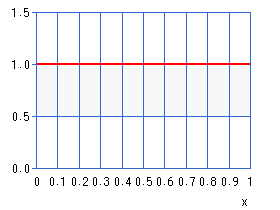
\includegraphics[width=\textwidth]{images/beta_1_1.png}
            \caption{$\alpha=1$, $\beta=1$}
            \label{sec:bhh:hyper_parameters:normalisation_beta_1_1}
      \end{subfigure}
      \begin{subfigure}{0.5\textwidth}
            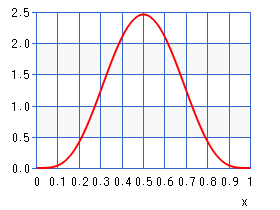
\includegraphics[width=\textwidth]{images/beta_5_5.png}
            \caption{$\alpha=5$, $\beta=5$}
            \label{sec:bhh:hyper_parameters:normalisation_beta_5_5}
      \end{subfigure}
      \par\bigskip
      \begin{subfigure}{0.5\textwidth}
            \centering
            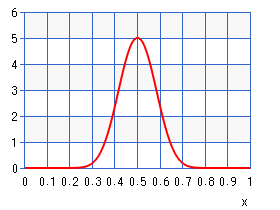
\includegraphics[width=\textwidth]{images/beta_20_20.png}
            \caption{$\alpha=20$, $\beta=20$}
            \label{sec:bhh:hyper_parameters:normalisation_beta_20_20}
      \end{subfigure}
      \par\bigskip
      \caption{Beta probability distribution with varying $\alpha$ and $\beta$ values.}
      \label{sec:bhh:hyper_parameters:discounted_rewards:normalisation}
\end{figure}

This concludes the hyper-parameters that are used by the \ac{BHH}. The following section discusses the default value for proxied update step operations.

\subsection{Defaults}
\label{sec:bhh:hyper_parameters:defaults}

Section \ref{sec:bhh:heuristic:proxies} provided the reader with the concept of proxied heuristic update step operations. As was mentioned in Section \ref{sec:bhh:hyper_parameters:heuristic_pool}, low-level heuristics each have their own set of hyper-parameters as well. This means that a set of default low-level parameters must be allocated specifically for these proxies. Consider a scenario where two instances of \ac{Adam} is included in the heuristic pool. Each has its own set of hyper-parameters that (should) differ from each other. In the case of \ac{Adam}, there are 4 hyper-parameters that include learning rate, $\beta1$, $\beta2$ and $\epsilon$. If another heuristic needs to proxy \ac{Adam}'s ``expected gradient mean operation'', a default $\beta1$ parameter must be supplied. Notice that this is only the case where multiple instances of a heuristic is included and there is uncertainty about which instance's hyper-parameters to use for the proxied heuristic update steps. If there is only one instance of a particular heuristic, that instance's hyper-parameters are used. The next section provides the reader with the pseudo-code algorithm for the \ac{BHH}.

\section{Algorithm}
\label{sec:bhh:algorithm}

This section provides the reader with a high level pseudo-code implementation of the \ac{BHH}. This is given in Algorithm \ref{algo:bhh} below.

\begin{algorithm}[H]
      \caption{The pseudo code for the \index{Bayesian Hyper-Heuristic} Bayesian Hyper-Heuristic optimiser}
      \label{algo:bhh}
      \begin{algorithmic}
            \State step $\gets 0$

            \State select initial heuristics
            \State initialise population and entities
            \State evaluate entities' initial position
            \State update population state

            \While{stopping condition not met}
            \For{all entities in entity pool}
            \If{selected heuristic is gradient-based}
            \State get gradients
            \EndIf

            \State apply low-level heuristic and proxy operations
            \State update population state
            \State log performance to performance log

            \If {step < burn-in window size}
            \State select heuristic
            \Else
            \If {step $\mathbin{\%}$ reanalysis window size = 0}
            \State apply Bayesian analysis
            \EndIf

            \If {step $\mathbin{\%}$ reselection window size = 0}
            \State select heuristic
            \EndIf

            \If {step > replay window size}
            \State prune performance log
            \EndIf
            \EndIf
            \EndFor
            \State step $\gets$ step + $1$
            \EndWhile
      \end{algorithmic}
\end{algorithm}

\section{Summary}
\label{sec:bhh:summary}

This chapter provided the reader with extensive detail on the inner workings and design of the \ac{BHH}. The \ac{BHH} was formally classified and the details around various components of the \ac{BHH}'s architecture was presented. Formal mathematical descriptions of the Bayesian selection method have been provided. The optimisation process, by means of Bayesian analysis has been presented and a pseudo code implementation of the \ac{BHH} was presented.

This concludes the background information and literature studies that is required to propose a methodology for an empirical process. This methodology is provided in the next chapter.

\chapter{Methodology}
\label{chap:methodology}

\begin{quote}
      \textit{Observation, reason and experimentation make up what we call the scientific method. $\sim$ Richard P. Feynman}
\end{quote}


Chapter \ref{chap:introduction} set out the objectives of the dissertation. These objectives can broadly be split between background information and an empirical component. So far, chapters \ref{chap:introduction}-\ref{chap:bhh} provided the necessary background information. This chapter now provides the detailed specification of the methodology that is followed for the empirical process and the analysis of the results. The remainder of the chapter is structured as follows:

\begin{itemize}
      \item \textbf{Section \ref{sec:methodology:overview}} provides a brief overview of the entire empirical process, leaving the detail to subsequent sections.

      \item \textbf{Section \ref{sec:methodology:datasets}} presents the detail around the datasets that are used.

      \item \textbf{Section \ref{sec:methodology:model}} provides the details of the models (\acs{FFNN}s) that are being trained.

      \item \textbf{Section \ref{sec:methodology:heuristics}} presents the detail around the different \index{heuristic}heuristics that are used along with their hyper-parameters.

      \item \textbf{Section \ref{sec:methodology:baseline_bhh}} provides the detail of the configuration of the \acs{BHH} baseline.

      \item \textbf{Section \ref{sec:methodology:performance_measures}} sheds light into the performance evaluation measures that are used.

      \item \textbf{Section \ref{sec:methodology:stopping_conditions}} discusses the stopping conditions that are used.

      \item \textbf{Section \ref{sec:methodology:experiments}} presents the different experimental groups that is executed.

      \item \textbf{Section \ref{sec:methodology:implementation}} sheds some light as to the implementation and execution of the empirical process.

      \item \textbf{Section \ref{sec:methodology:statistical_analysis}} presents the procedures that are followed in during the statistical analysis of the results.

      \item Finally, a summary of the chapter is provided in \textbf{Section \ref{sec:methodology:summary}}
\end{itemize}

\section{Overview of Empirical Process}
\label{sec:methodology:overview}

The purpose of the empirical process is to present and execute a carefully crafted experiment/test that produces data that can be used to reject of verify some hypothesis about the element under investigation. This dissertation has outlined a set of 3 objectives that require such empirical processes to evaluate the \ac{BHH}. This section outlines what these empirical processes entail.

Each empirical test sets out some configuration of elements to be evaluated. These generally include a set of parameters that are altered between experiments. Each experiment is evaluated by means of a performance measurement. In the context of training \acp{FFNN}, the underlying model (\ac{NN}) is trained across a number of datasets. Each dataset is split into a training and test set. The training set is used to train the model, while the test set is used to evaluate the model. Training epochs are split into mini-batch iterations, with each dataset containing a specified mini-batch size. Evaluation takes place at every mini-batch step. These experiments contain a number of components, each with a set of paramaters. Due to the stochastic nature of the experiments, each experiment is repeated over a number of runs to provide sufficient sample for statistical certainty. Each run contains a different random seed. Each evaluation's results are analysed for statistical significance. It is from these statistical analyses that findings and conclusions are then made.

Detail around each of these elements are now provided, starting with the datasets that are used.

\section{Datasets}
\label{sec:methodology:datasets}

This section provides the detail around the different datasets that are used throughout the empirical process. These datasets originate from the UCI Machine Learning Repository~\cite{ref:uci:2022}. Datasets are grouped by problem type and include 8 classification and 7 regression datasets. The classification datasets are given in Table \ref{tab:methodology:datasets:classification} and the regression datasets are given in Table \ref{tab:methodology:datasets:regression} below.

\begin{table}[htbp]
      \centering
      \caption{Classification datasets}
      \label{tab:methodology:datasets:classification}%
      \par\bigskip
      \resizebox{\textwidth}{!}{
            \begin{tabular}{ccccccccc}
                  \textbf{dataset} & \textbf{output} & \textbf{types}             & \textbf{attributes} & \textbf{classes} & \textbf{instances} & \textbf{batch} & \textbf{steps} & \textbf{citation}          \\
                  \midrule
                  iris             & multivariate    & real                       & 4                   & 3                & 150                & 16             & 10             & ~\cite{ref:fisher:1936}    \\
                  car              & multivariate    & categorical                & 6                   & 4                & 1728               & 128            & 14             & ~\cite{ref:bohanec:1988}   \\
                  abalone          & multivariate    & categorical, integer, real & 8                   & 28               & 4177               & 256            & 17             & ~\cite{ref:waugh:1995}     \\
                  mushroom         & multivariate    & categorical                & 22                  & 2                & 8214               & 512            & 17             & ~\cite{ref:schlimmer:1987} \\
                  wine\_quality    & multivariate    & real                       & 12                  & 11               & 4898               & 256            & 20             & ~\cite{ref:cortez:2009}    \\
                  bank             & multivariate    & real                       & 17                  & 2                & 45211              & 512            & 89             & ~\cite{ref:moro:2014}      \\
                  diabetic         & multivariate    & integer                    & 55                  & 3                & 100000             & 1024           & 98             & ~\cite{ref:strack:2014}    \\
                  adult            & multivariate    & categorical, integer       & 14                  & 2                & 48842              & 256            & 191            & ~\cite{ref:kohavi:1996}    \\
            \end{tabular}%
      }
\end{table}%

\begin{table}[htbp]
      \centering
      \caption{Regression datasets}
      \label{tab:methodology:datasets:regression}%
      \par\bigskip
      \resizebox{\textwidth}{!}{
            \begin{tabular}{cccccccc}
                  \textbf{dataset}     & \textbf{output}          & \textbf{types} & \textbf{attributes} & \textbf{instances} & \textbf{batch} & \textbf{steps} & \textbf{citation}         \\
                  \midrule
                  fish\_toxicity       & multivariate             & real           & 7                   & 908                & 64             & 15             & ~\cite{ref:cassotti:2015} \\
                  housing              & univariate               & real           & 13                  & 506                & 32             & 16             & ~\cite{ref:harrison:1978} \\
                  forest\_fires        & multivariate             & real           & 13                  & 517                & 32             & 17             & ~\cite{ref:cortez:2007}   \\
                  student\_performance & multivariate             & integer        & 33                  & 649                & 32             & 21             & ~\cite{ref:cortez:2008}   \\
                  parkinsons           & multivariate             & integer, real  & 26                  & 5875               & 256            & 23             & ~\cite{ref:tsanas:2009}   \\
                  air\_quality         & multivariate, timeseries & real           & 15                  & 9358               & 256            & 37             & ~\cite{ref:de:2008}       \\
                  bike                 & univariate               & integer, real  & 16                  & 17389              & 256            & 68             & ~\cite{ref:fanaee:2014}   \\
            \end{tabular}%
      }
\end{table}%

Details on how the datasets where preprocessed and prepared is given in Appendix \ref{app:datasets}. The concept of class balancing is briefly discussed next.

\subsection{Class Balancing}

A number of classification datasets as given in Table \ref{tab:methodology:datasets:classification} above contain unbalanced classes. A decision was made to not make use of class balancing. This was simply to eliminate as many variables adn factors in the empirical process as possible, as it is already a complicated process.  It is therefore suggested that the \ac{BHH} first be studied under the assumption of balanced classes and then only apply class balancing. In future research opportunities, class balancing should be utilised.

The next section presents the models and the configurations that are used.


\section{Models}
\label{sec:methodology:model}

As the title of the dissertation suggests, these empirical process are focused on the training of \acp{FFNN}. In theory, one should be able to swap these \acp{FFNN} out for any other mathematical model that can be optimised. All models that are trained in this dissertation are shallow \acp{NN}, meaning they only have one hidden layer. The architecture of a model is dependent on the dataset being trained on, the type of problem it is (classification or regression), the number of input dimensions and the number of output dimensions. The models and their configuration, as it is used for each dataset, is given below in Table \ref{tab:methodology:models:configurations}


% Table generated by Excel2LaTeX from sheet 'Model Configurations'
\begin{table}[htbp]
      \centering
      \caption{Model configurations}
      \label{tab:methodology:models:configurations}%
      \par\bigskip
      \resizebox{\textwidth}{!}{
            \begin{tabular}{rcccccccc}
                  \textbf{dataset}     & \textbf{inputs} & \textbf{hidden} & \textbf{output} & \textbf{biases} & \textbf{parameters} & \textbf{topology} & \textbf{l1 activation} & \textbf{l2 activation} \\
                  \midrule
                  fish\_toxicity       & 6               & 3               & 1               & yes             & 25                  & dense             & LReLU ($\alpha = 0.3$) & sigmoid                \\
                  iris                 & 4               & 5               & 3               & yes             & 43                  & dense             & LReLU ($\alpha = 0.3$) & softmax                \\
                  air\_quality         & 12              & 8               & 1               & yes             & 113                 & dense             & LReLU ($\alpha = 0.3$) & sigmoid                \\
                  housing              & 13              & 8               & 1               & yes             & 121                 & dense             & LReLU ($\alpha = 0.3$) & sigmoid                \\
                  wine\_quality        & 13              & 10              & 7               & yes             & 217                 & dense             & LReLU ($\alpha = 0.3$) & softmax                \\
                  parkinsons           & 21              & 10              & 1               & yes             & 231                 & dense             & LReLU ($\alpha = 0.3$) & sigmoid                \\
                  car                  & 21              & 10              & 4               & yes             & 264                 & dense             & LReLU ($\alpha = 0.3$) & softmax                \\
                  forest\_fires        & 43              & 16              & 1               & yes             & 721                 & dense             & LReLU ($\alpha = 0.3$) & sigmoid                \\
                  abalone              & 10              & 36              & 28              & yes             & 1432                & dense             & LReLU ($\alpha = 0.3$) & softmax                \\
                  bank                 & 51              & 32              & 1               & yes             & 1697                & dense             & LReLU ($\alpha = 0.3$) & softmax                \\
                  bike                 & 61              & 32              & 1               & yes             & 2017                & dense             & LReLU ($\alpha = 0.3$) & sigmoid                \\
                  student\_performance & 99              & 32              & 1               & yes             & 3233                & dense             & LReLU ($\alpha = 0.3$) & sigmoid                \\
                  adult                & 108             & 64              & 1               & yes             & 7041                & dense             & LReLU ($\alpha = 0.3$) & softmax                \\
                  mushroom             & 117             & 64              & 1               & yes             & 7617                & dense             & LReLU ($\alpha = 0.3$) & softmax                \\
                  diabetic             & 2369            & 32              & 3               & yes             & 75939               & dense             & LReLU ($\alpha = 0.3$) & softmax                \\
            \end{tabular}%
      }
\end{table}%

It should be noted that for the classification problems, the \index{softmax}softmax activation is not actually part of the model. It is just added for predictive output and is not needed during evaluation. The loss functions (\ac{SparseCatXE} and \ac{BinXE}) that are used contains a \index{softmax}softmax function. Models' initial weights are initialised by means of \index{Glorot uniform sampling}Glorot uniform sampling.

\section{Heuristics/Optimisers}
\label{sec:methodology:heuristics}

This section provides the details of the standalone \index{heuristic}heuristics/optimisers that are used in the empirical process.

Table \ref{tab:methodology:heuristics} contain a list of all the standalone \index{heuristic}heuristics that are used as well as their hyper-parameter configuration.

% Table generated by Excel2LaTeX from sheet 'BHH Baseline'
\begin{table}[htbp]
      \centering
      \caption{Heuristics/optimisers and their hyper-parameter configuration of their}
      \label{tab:methodology:heuristics}%
      \par\bigskip
      \resizebox{0.8\textwidth}{!}{

            \begin{tabular}{llll}
                  \textbf{heuristic} & \textbf{configuration}    & \textbf{value} & \textbf{citation}          \\
                  \midrule
                  sgd                & learning\_rate            & 0.1**0.01      & ~\cite{ref:sutskever:2013} \\
                  momentum           & learning\_rate            & 0.1**0.01      & ~\cite{ref:sutskever:2013} \\
                                     & momentum                  & 0.9            &                            \\
                  nag                & learning\_rate            & 0.1**0.01      & ~\cite{ref:sutskever:2013} \\
                                     & momentum                  & 0.9            &                            \\
                  adagrad            & learning\_rate            & 0.1**0.01      & ~\cite{ref:duchi:2011}     \\
                                     & epsilon                   & 1E-07          &                            \\
                  rmsprop            & learning\_rate            & 0.1**0.01      & ~\cite{ref:hinton:2012}    \\
                                     & rho                       & 0.95           &                            \\
                                     & epsilon                   & 1E-07          &                            \\
                  adadelta           & learning\_rate            & 1.0**0.95      & ~\cite{ref:zeiler:2012}    \\
                                     & rho                       & 0.95           &                            \\
                                     & epsilon                   & 0.0000001      &                            \\
                  adam               & learning\_rate            & 0.1**0.01      & ~\cite{ref:kingma:2014}    \\
                                     & beta1                     & 0.9            &                            \\
                                     & beta2                     & 0.95           &                            \\
                                     & epsilon                   & 1E-07          &                            \\
                  pso                & population\_size          & 10             & ~\cite{ref:van:2010}       \\
                                     & learning\_rate            & 0.1**0.01      &                            \\
                                     & inertia\_weight (w)       & 0.729844       &                            \\
                                     & cognitive\_control (c1)   & 1.49618        &                            \\
                                     & social\_control (c2)      & 1.49618        &                            \\
                                     & velocity\_clip\_min       & -1.0           &                            \\
                                     & velocity\_clip\_max       & 1.0            &                            \\
                  de                 & population\_size          & 10             & ~\cite{ref:mezura:2006}    \\
                                     & selection\_strategy       & best           &                            \\
                                     & xo\_strategy              & exp            &                            \\
                                     & recombination probability & 0.9**0.1       &                            \\
                                     & beta                      & 2.0**0.1       &                            \\
                  ga                 & population\_size          & 10             & ~\cite{ref:lambora:2019}   \\
                                     & selection\_strategy       & rand           &                            \\
                                     & xo\_strategy              & bin            &                            \\
                                     & mutation\_rate            & 0.2**0.05      &                            \\
            \end{tabular}%
      }
\end{table}%

Take note that for Table \ref{tab:methodology:heuristics}, values that contains an asterisk ($*$) are configured on a schedule with the initial value depicted first and the decay rate is depicted last. The number of steps is the total number of steps for that particular dataset it is being applied to.

Also take note that a learning rate was added to the \ac{PSO} as an attempt to avoid overshooting solutions later in the training process. This parameter does not traditionally form part of the \ac{PSO}, but it was found to work sufficiently here.

The next section provides the details around the \ac{BHH} baseline.



















TODO: Proxy Mapping Table



























\section{BHH Baseline}
\label{sec:methodology:baseline_bhh}

The \ac{BHH} baseline is a name given to a specific configuration of the \ac{BHH}, which during development, has been found to provide reasonable performance. It was decided that this configuration will be the cornerstone configuration from which all other \index{heuristic}heuristics and their configurations are evaluated. The \ac{BHH} baseline represents the main component that is evaluated in this dissertation. The configuration for the \ac{BHH} baseline is given in Table \ref{tab:methodology:bhh_baseline_configuration} below:

% Table generated by Excel2LaTeX from sheet 'BHH Baseline'
\begin{table}[htbp]
      \centering
      \caption{BHH baseline configurations}
      \label{tab:methodology:bhh_baseline_configuration}%
      \par\bigskip
      \resizebox{0.8\textwidth}{!}{
            \begin{tabular}{rrcc}
                  \multicolumn{1}{c}{\textbf{hyper-heuristic}} & \multicolumn{1}{c}{\textbf{variant}} & \textbf{configuration} & \textbf{value} \\
                  \midrule
                  \multicolumn{1}{l}{bhh}                      & \multicolumn{1}{l}{baseline}         & heuristic\_pool        & all            \\
                                                               &                                      & population             & 5              \\
                                                               &                                      & credit                 & ibest          \\
                                                               &                                      & reselection            & 10             \\
                                                               &                                      & replay                 & 10             \\
                                                               &                                      & reanalysis             & 10             \\
                                                               &                                      & normalise              & false          \\
                                                               &                                      & discounted\_rewards    & false          \\
            \end{tabular}%
      }
\end{table}%

Table \ref{tab:methodology:bhh_baseline_configuration} refers to the \index{heuristic}heuristic pool that is used as \textit{all}. This refers to a configuration where the heuristic pool contains all the low-level heuristics as presented in Section \ref{sec:methodology:heuristics}. This list of low-level \index{heuristic}heuristics naturally also then form the list of standalone heuristics/optimisers to which the \ac{BHH} is compared and analysed as is described later in  Section \ref{sec:methodology:experiments:standalone_optimisers}. Specifically the finer details of the implementation of the \ac{BHH}, the low-level \index{heuristic}heuristic pool and how it is used is given in Chapter \ref{chap:bhh}.


\section{Performance Measures}
\label{sec:methodology:performance_measures}

This section sheds light into the performance measures that are used to evaluate the different experimental runs.

Chapter \ref{chap:anns} provided the reader with a number of techniques that are used to evaluate \ac{FFNN} performance during training. Broadly these techniques measure the output of some loss/cost function and accuracy for classification problems. For the classifications problems, the loss metrics used included \ac{SparseCatXE} and \ac{BinXE}. Their accuracy equivalent metrics are then also used. For regression problems, \ac{RMSE} is used as a loss metric.

As mentioned in the preceding sections, datasets are split into a training set and a test dataset. The training set is used to train the model and the test set is used to test the model. Evaluation takes place at the end of each mini-batch iteration. Loss and accuracy is measured for both training and test datasets and is captured at each mini-batch iteration.

Post processing of the results yield a average rank (by test loss metric) between configurations at each mini-batch step across all runs. This test loss metric and rank then form experimental results that are then statistically analysed.

\section{Stopping Conditions}
\label{sec:methodology:stopping_conditions}

This section sheds light on the stopping conditions that are used.

Early stopping is a technique where training is prematurely stopped due to training saturation. A popular technique for early stopping includes a check to see if the validation/test loss has improved in the last $k$ steps. If the loss has not improved, the training is halted and the last best model weights are used.

It was decided not to use early stopping in this empirical process. Since the \ac{BHH} is a novel \ac{HH}, there are lots of uncertainty around its performance. It is unsure as to how the \ac{BHH} will behave, should overfitting take place. By eliminating early stop, the \ac{BHH} is evaluated until a maximum number of epochs (30) is reached. It is recommended that future research make use of early stopping.

The different experimental groups are given next.







\section{Experiments}
\label{sec:methodology:experiments}

This section presents the experimental groups that form part of the empirical process. There are broadly 3 main groups. These include a behavioural case study, a critical evaluation of the \ac{BHH} baseline's performance compared to other standalone low-level \index{heuristic}heuristics and finally an analysis of different \ac{BHH} variants is done by analysing the effects of different parameter values on the outcomes of the \ac{BHH}. Each of these sections are discussed in more detail below.


\subsection{Behavioural Case Study}
\label{sec:methodology:experiments:case_study}

This experimental group is concerned with objectively studying the behaviour of the \ac{BHH} baseline across a number of runs. This is meant to be an introductory analysis of the \ac{BHH} and includes analysis of the selection mechanism as well as the perturbative nature of the \ac{BHH}. It is important to mention that this experimental group is not meant to be statistically analysed, but to rather provide a detailed visual analysis of a number of hand-picked example runs, to determine if the \ac{BHH} is behaving as expected. It also provides a gentle introduction to the \ac{BHH}'s inner workings. From these observations, it is determined if the \ac{BHH} is learning and that selection is indeed biasing towards better performance. It also provides an opportunity to determine the outcome of the perturbative component of the \ac{BHH} which includes proxied \index{heuristic}heuristic update step operations.

Two different configurations of the \ac{BHH} baseline is trained using the iris dataset~\cite{ref:fisher:1936}. These configurations include a replay window size of 10 (short memory) and a high replay window size of 250 (long memory). Each configuration is repeat 3 times. Finally these configurations are compared to a run that is purely random.

The analysis is primarily done by dissecting the output of various parameters and studying the plots of their values. From these plots, conclusions about the \ac{BHH}'s behaviour is made.

\subsection{Standalone Optimisers}
\label{sec:methodology:experiments:standalone_optimisers}

THis section presents the details with the experimental group that focuses on evaluating the performance of the \ac{BHH} with that of standalone \index{heuristics}/optimisers.

For this experimental group, the heuristics and optimisers as presented in Section \ref{sec:methodology:heuristics} are used, along with their specified parameters. Each of these are then compared to that of the \ac{BHH} baseline configuration which is presented in Section \ref{sec:methodology:baseline_bhh}.

The next section provides the details around different \ac{BHH} variants that are evaluated.

\subsection{BHH Variants}
\label{sec:methodology:experiments:bhh_variants}

This section provides the details of the experimental group that focuses on \ac{BHH} variants and the effect that different hyper-parameter configurations can have on the outcome of the \ac{BHH}.

The different variants and their possible configurations is given in Table \ref{tab:methodology:experiments:bhh_variants} below.

\begin{table}[htbp]
      \centering
      \caption{BHH variants and their configuration}
      \label{tab:methodology:experiments:bhh_variants}%
      \par\bigskip
      \resizebox{0.9\textwidth}{!}{
            \begin{tabular}{rcc}
                  \multicolumn{1}{c}{\textbf{hyper-heuristic}} & \textbf{variant}    & \textbf{values}                   \\
                  \midrule
                  \multicolumn{1}{l}{bhh}                      & heuristic\_pool     & all,gd,mh                         \\
                                                               & population          & 5,10,15,20,25                     \\
                                                               & credit              & ibest,pbest,rbest,gbest,symmetric \\
                                                               & reselection         & 1,5,10,15,20                      \\
                                                               & replay              & 1,5,10,15,20                      \\
                                                               & reanalysis          & 1,5,10,15,20                      \\
                                                               & burn\_in            & 0,5,10,15,20                      \\
                                                               & normalise           & false,true                        \\
                                                               & discounted\_rewards & false,true                        \\
            \end{tabular}%
      }
\end{table}%

Take note that the \index{heuristics}heuristic pool options \textit{gd} and \textit{mh} refers to the \index{heuristics}heuristic pool configurations where the heuristic pools contain only gradient-descent heuristics or only \{index{meta-heuristics}meta-heuristics  respectively.

The next section explains in detail how the results are statistically analysed.

\section{Statistical Analysis}
\label{sec:methodology:statistical_analysis}

This section provides the detail of the process that is used to execute the statistical analysis of the results.

Various experimental groups and the details of the configuration is given in the preceding sections. Each of these experimental groups are statistically analysed on their own. To ensure there is statistically sufficient sample, each experimental group and configuration is trained for 30 epochs, repeated over 30 runs. As it is mentioned above, the results contain performance evaluation data in the form of training and testing, loss and accuracy measurements. Each experimental run is then ranked by these metrics. Each run is executed using a unique seeding value such such that each run is identical in its setup and configuration (apart from seeding values) and independent of the other runs.

Each experimental group goes through a set of steps that are followed during the statistical analysis process. First, the descriptive analysis is done to ensure that each experiment has the required data it needs. This includes 30 runs per configuration, across 15 datasets, across the applicable number of experimental configurations set up by that particular experimental group. The spread of the data is analysed to evaluate for overfit and outliers are identified. The skewness of the results is evaluated per dataset and the \index{Shapiro-Wilk}Shapiro-Wilk test for normality ($\alpha$ = 0.001) is used to determine in the results are normally distributed. The full statistical analysis reports are presented in Appendix \ref{app:statistical_analysis} and provides descriptive plots of the data's distribution. Furthermore, the \index{Levene}Levene's test for equality of variance ($\alpha$ = 0.001) is used.

Dependent on the outcomes of the above statistical tests, the appropriate statistical significance test is then executed. For configurations of independent variables where there are only 2 classes, the Mann-Whitney U\index{Mann-Whitney U} independent samples t-Test ($\alpha$ = 0.001) is executed and for configurations of 3 or more configuration classes, the \ac{ANOVA} statistical test ($\alpha$ = 0.001) is used. The\index{Kruskal-Wallis} Kruskal-Wallis ranked non-parametric test for statistical significance ($\alpha$ = 0.001) is used for cases where data is not normally distributed.

As mentioned earlier in the chapter, results are analysed for statistical significance over all the steps during the training process across all runs. This helps determine if there is statistical difference in the execution of various experimental configurations, throughout the entire training process, but also to cater for overfitting, which is to be studied as well.

Regardless of the statistical test that is used, a post-hoc Tukey honest significant difference test ($\alpha$ = 0.001) is used from which significant ranking is retrieved. Descriptive and critical difference plots are then retrieved from these results to provide visual aid, but all conclusions are made from statistically analysed data as mentioned above.

\section{Implementation and Execution}
\label{sec:methodology:implementation}

This section sheds some light as to the details of the implementation and execution of the empircal process.

All implementation is done from first principles in Python 3.9 using Tensorflow 2.7 and Tensorflow Probability 0.15.0. Most underlying function are reused from the Tensorflow library, however, all heuristics/optimisers are implemented from first principles to fit the \ac{HH} framework that was developed. All source code and data is provided is resources in this dissertation.

It should be noted that this implementation makes heavy use of CPU processing, due to the nature of modeling flattening for the \index{heuristic}heuristics. For this reason, execution is much more timely and costly than with GPU training. The authors hope that as the \ac{BHH} evolves, that better GPU implementations may speed up execution times.

With regards to the computational power that was used the execute this empirical process. All experiments were run on the CHPC's cluster. This included 14 servers each running 24-56 cores and 256GB memory each. The entire empirical process took 6 days.

\section{Summary}
\label{sec:methodology:summary}

This chapter provided the detail around the methodology that is used to execute the empirical process. The datasets, models and heuristics that are used during the empirical process have been presented in detail. A baseline \ac{BHH} has been formulated. The empirical process was defined in terms of a number of different experiments and finally, the process of statistical analysis of the results was provided.

The results and findings of the empirical process are presented in the following chapter.

\chapter{Results}
\label{chap:results}


\begin{quote}
	\textit{
		``Without data, you are just another person with an opinion.'' - W. Edwards Deming
	}
\end{quote}

The last step in the scientific process requires the presentation and objective discussion of empirical findings with good statistical backing. From the problem statements and motivations made in Chapter \ref{chap:introduction}, goals have been defined that broadly include literature studies and a sound empirical process. Thus far, the reader has been provided with a vast scope of background information relevant to the development of the \Acs{BHH}. Chapters \ref{chap:introduction} - \ref{chap:probability} provided the background information, literature studies and existing landscape of research for \acp{ANN}, \index{heuristic}heuristics/\index{optimiser}optimisers, \acp{HH} and probability theory. These elements all share common elements that are required to understand the proposed \Acp{BHH} which was presented in Chapter \ref{chap:bhh}. The details around the empirical process was formally proposed in the methodology as presented in Chapter \ref{chap:methodology}. Finally, the results for the empirical process can be presented and this chapter aims to provide these results.

As a reminder, the empirical process is split into two main experimental groups. These include a behavioural case study and set of comparative studies. This chapter is organised into the same logical pattern. Each of these experimental groups is provided as its own section for detailed analysis and discussion of findings. The remainder of the chapter is structured as follows:

\begin{itemize}
	\item \textbf{Section \ref{sec:results:overview}} provides a brief overview of the general empirical process, high level discussion points and a brief discussion on results interpretation.

	\item \textbf{Section \ref{sec:results:case_study}} provides a detailed analysis of the behaviour of the \Acs{BHH} over a few example runs during training and testing and is meant to introduce the analysis of the \Acs{BHH} from a behavioural characteristic point of view. In this section, focus is put on the learning process itself and to determine what happens during training. It aims to provide insight into ``how'' and ``when'' the \Acs{BHH} learning happens.

	\item \textbf{Section \ref{sec:results:standalone}} provides the first of a series of comparative studies. This section presents the comparative analysis that studies the performance capabilities of the baseline configuration of the \Acs{BHH} to that of standalone/individual low level \index{heuristic}heuristics/\index{optimiser}optimisers. The sections that follow focus on the effect of various parameters on the \Acs{BHH}.

	\item \textbf{Sections \ref{sec:results:heuristic_pool}} - \ref{sec:results:discounted_rewards} capture the results of these empirical processes and focus on the configuration of the \textit{heuristic pool}, the \textit{population size}, \textit{credit assignment strategies}, \textit{reselection} window size, \textit{replay} window size, \textit{reanalysis} window size, \textit{burn in}, \textit{normalisation} and \textit{discounted rewards}, respectfully.

	\item \textbf{Section \ref{sec:results:computational_requirements}} contains a brief discussion on the computational requirements.

	\item \textbf{Section \ref{sec:results:overfitting}} provides a brief discussion on overfitting.

	\item Finally, a summary of the findings is given in \textbf{Section \ref{sec:results:summary}}.
\end{itemize}

\section{Overview}
\label{sec:results:overview}

This section aims to provide a general high level discussion on the outcomes of the empirical process as an introduction to the more detailed discussions to follow. Consider again the goals that have been defined in \ref{chap:introduction}. The empirical component addresses three different angles of analysis:

\begin{enumerate}
	\item Analysing the behaviour of the \Acs{BHH} during training and testing to determine if the the concept works and that the \Acs{BHH} is indeed learning. This component looks at the \Acs{BHH} in isolation and simply evaluates the outcomes of its behaviour over a few example runs and repeats this process for two groups of \Acs{BHH} variants based on \textit{replay} window size.

	\item Comparing the performance capabilities of the \Acs{BHH} to that of well-known low-level \index{heuristic}heuristics that are well researched and understood. This component looks at how the \Acs{BHH} performs given a frame of reference to compare to. Careful consideration of results interpretation must be given here and is discussed in more detail below.

	\item Analysing the effects of various configurations of hyper-parameters for the \Acs{BHH}. This component looks at which parameters have a statistically significant impact on the outcomes of the \Acs{BHH}.
\end{enumerate}

It is important to briefly discuss how results should be interpreted. Traditionally, for typical low-level heuristic training, evaluation of performance is done at a chosen point in time and based on a particular dependent variable. This could be a fixed number of training steps/epochs, early stopped conditions or any other stopping condition. The metric of interest could be a loss value, an accuracy or a rank. Algorithms/heuristics in question are then logically ranked/organised according to their final solution and conclusions are made based on these findings. However, the following arguments suggest an alternative approach for this empirical study:

\begin{itemize}
	\item
	      Since there does not exist any research on this specific implementation of \acp{HH} and its application to \acs{FFNN} training, there is no clear point at which it is known that the learning of the \acs{BHH} becomes detrimental to the training process. For example, there exists a currently unknown point during training where the performance bias towards the ``best'' \index{heuristic}heuristic no longer yield improved training or test generalisation outcomes. To cater for this, a fixed maximum number of training epochs have been chosen that empirically have been shown to be sufficient to notice diminishing returns in the outcome. \index{Early stopping}Early stopping was considered, but purposefully not implemented. This is to allow the study of the behaviour and capabilities of the \Acs{BHH} up to and beyond the point of diminishing returns.

	\item
	      The training process is to some degree analogous and comparable to a dynamic optimisation problem as previously discussed. This means that the performance of \index{heuristic}heuristics, and thus the \Acs{BHH}, vary at different times during the training process. This hints to the hypothesis that was set in Chapter \ref{chap:introduction} and suggests that there is no single \index{heuristic}heuristic that is always the best \index{heuristic}heuristic to use during all of training. Rather, there exists an applicable, relevant \index{heuristic}heuristic (or combination of \index{heuristic}heuristics) to use at a given point in time during the training process and can change as the process continues. This means the selected \index{heuristic}heuristic at time step $t$ is not necessarily the best heuristic to select at timestamp $t+1$. This argument is further supported by the fact that these experiments are trained on mini-batches, resulting in a lot of noise during training. This noise can cause the \Ac{BHH} to want to "correct" a certain learnt belief. This introduces the same challenges as with \Ac{RL}: Consider delayed rewards, size of rewards, unlearning behaviour that is no longer required, all of which affect the training process throughout and not just at the point of stopping.
\end{itemize}


Based on the points made above, each experimental group is to be evaluated in isolation and has a specific area of focus. For all experimental groups, heuristics are evaluated during \textbf{all} the steps of the training and testing process. For this reason, ranking \index{heuristic}heuristic should not necessarily lead to the conclusion that one heuristic is \textit{better} than another, but rather, that there is a statistically significant difference between the outcomes of heuristics, relative to the entire training and testing process for a given experimental group. The authors suggest further research to include early stopping conditions for the ranking to make entirely sense. However, that does not mean the ranking approach is useless. It still provides a measure of comparison and is indeed indicative of statistically significant outcomes.

The points that have been discussed above have been observed during the empirical process. It is shown in the succeeding sections that the \Acs{BHH} is capable of training \Acp{FFNN} and that it does so relatively well. It is shown that the \Acs{BHH} is generally capable of providing good test generalisations when compared to existing low-level \index{heuristic}heuristics. However, it is shown that the majority of the influence of the \Acs{BHH} occurs during the first few epochs of the training process. Initially uniformly randomised candidate solutions has more room to learn in the initial phases of training in comparison to later phases where learning has become stagnated. It is also shown that this pivotal point of diminishing return is problem specific. Further to this pivotal point, it is shown that the \Acs{BHH} is subject to over-fitting, quite drastically. There are various conclusions that can be made from this point, but the detail is left to the relevant sections to follow.

The following section provides the results and findings for a behavioural case study of the \Acp{BHH} on the iris dataset.


\section{Case Study}
\label{sec:results:case_study}

This section provides a study on the behaviour of the \Acs{BHH} during training and testing. It is important to mention that this experimental group does not necessarily focus on the exact metrics, but rather on the general behaviour of the \Ac{BHH}. This means that statistical analysis and statistical certainty as is not required. Instead, a number of example runs have been executed purely for the intent of analysing behaviour. Furthermore, this behavioural case study is executed on a very small, but well-known toy dataset called \textit{iris}. Iris is not usually considered for full empirical processes due to its size and simplicity. Although there are fourteen other datasets to choose from, iris provides a very simple, relevant and relate-able case study that illustrate the necessary points sufficiently.

Figure \ref{fig:results:case_study:iris:metric_plots} illustrate these runs during training and testing. Take note of the legend as provided in Figure \ref{fig:results:case_study:iris:legend}. There are two variants of the \Acs{BHH} included here, each with three repeated runs, seeded according to run number:

\begin{itemize}
	\item \Acp{BHH} with a very \textbf{short memory}, i.e. replay windows size = 10
	\item \Acp{BHH} with a very \textbf{long memory}, i.e. replay windows size = 250
\end{itemize}

These two groups have been chosen as their parameters have been shown to provide drastically different outcomes from each other during training and forms a good basis for behavioural analysis. For more details on replay window size, see Section \ref{sec:results:replay}.

A breakdown of the run notation as provided in Figure \ref{fig:results:case_study:iris:legend} is then given as follows:

\begin{itemize}
	\item \textbf{iris} - The dataset in question
	\item \textbf{bhh} - The heuristic in question
	\item \textbf{hp:all} - The heuristic pool (hp) in question. ``All'' refers to all the implemented lower-level heuristics including both classical gradient-based heuristics/optimisers as well as meta-heuristics.
	\item \textbf{ps:5} - The population size (ps) in question. In this case, population size = 5.
	\item \textbf{bi:0} - The burn in window size (bi) in question. In this case, burn in window size = 0.
	\item \textbf{rp:10} - The replay window size (rp) in question. In this case, replay window size = 10.
	\item \textbf{rs:10} - The reselection window size (rp) in question. In this case, reselection window size = 10.
	\item \textbf{ra:10} - The reanalysis window size (rp) in question. In this case, reanalysis window size = 10.
	\item \textbf{nm:False} - The normalisation flag (nm) in question. In this case, normalisation is disabled.
	\item \textbf{ct:ibest} - The credit assignment strategy (ct) in question. In this case, the credit assignment strategy used is \textit{ibest}.
	\item \textbf{dr:False} - The discounted rewards flag (dr) in question. In this case, discounted rewards is disabled.
\end{itemize}

From figure \ref{fig:results:case_study:iris:metric_plots} it is shown that the \Acs{BHH} exhibit similar behaviours to that of lower-level heuristics. Figures \ref{fig:results:case_study:iris:train:loss} and \ref{fig:results:case_study:iris:train:accuracy} illustrates a smooth training process, converging to a well-known minimum loss for the iris dataset. In Figures \ref{fig:results:case_study:iris:test:loss} and \ref{fig:results:case_study:iris:test:accuracy} it is shown that the \Acs{BHH} generalised well on the test set. Generalisation improved up to about epoch 10 before overfitting starts occurring. From this, it can be concluded that most of the learning, for this particular dataset, takes place in the first 10 epochs of the training process. From this point onwards, the \Acs{BHH} tries to undo ``bad'' selections made earlier. It is interesting to notice that despite overfitting, the \Acs{BHH} was able to ``correct'' itself to some degree (up to epoch 20), but never really converged back on the minimum it reached up to epoch 10. Early stopping should prohibit this from happening, but this is left for further research.

\begin{figure}[htbp]
	\begin{subfigure}{0.49\textwidth}
		\centering
		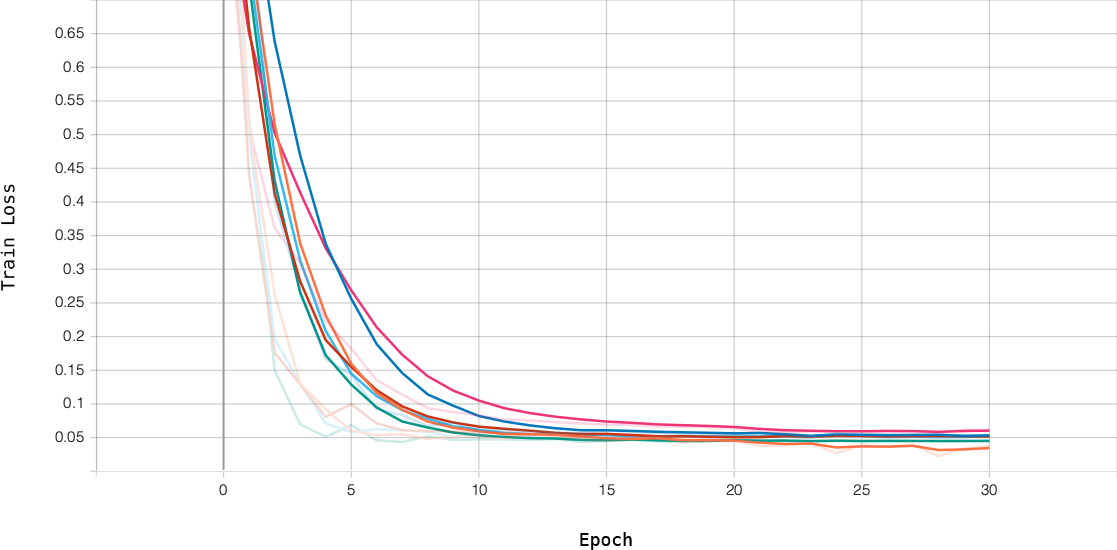
\includegraphics[width=\textwidth]{bhh_case_study/iris/train_loss.png}
		\caption{Train loss}
		\label{fig:results:case_study:iris:train:loss}
	\end{subfigure}
	\begin{subfigure}{0.49\textwidth}
		\centering
		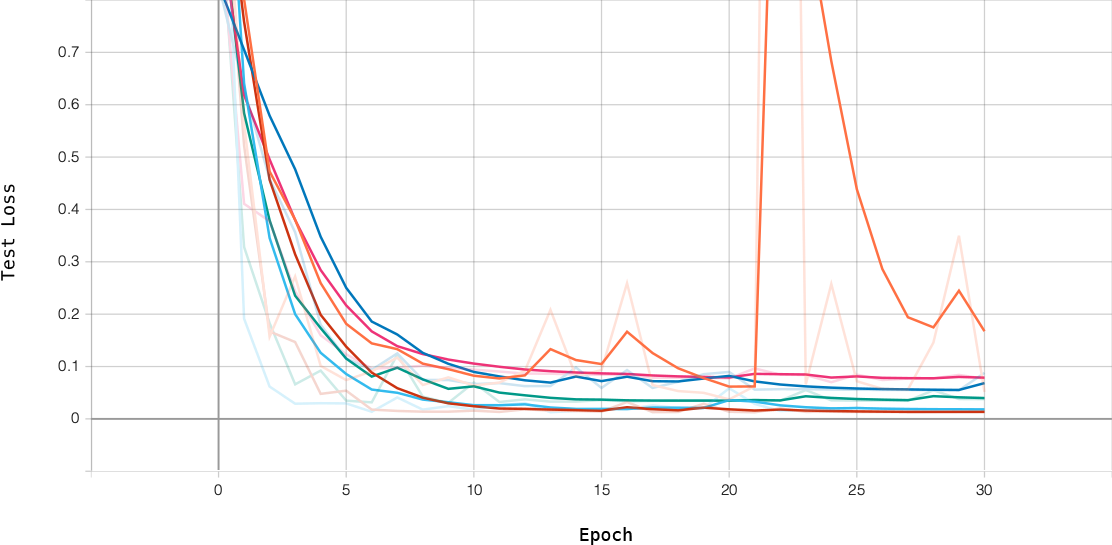
\includegraphics[width=\textwidth]{bhh_case_study/iris/test_loss.png}
		\caption{Test loss}
		\label{fig:results:case_study:iris:test:loss}
	\end{subfigure}
	\par\bigskip
	\begin{subfigure}{0.49\textwidth}
		\centering
		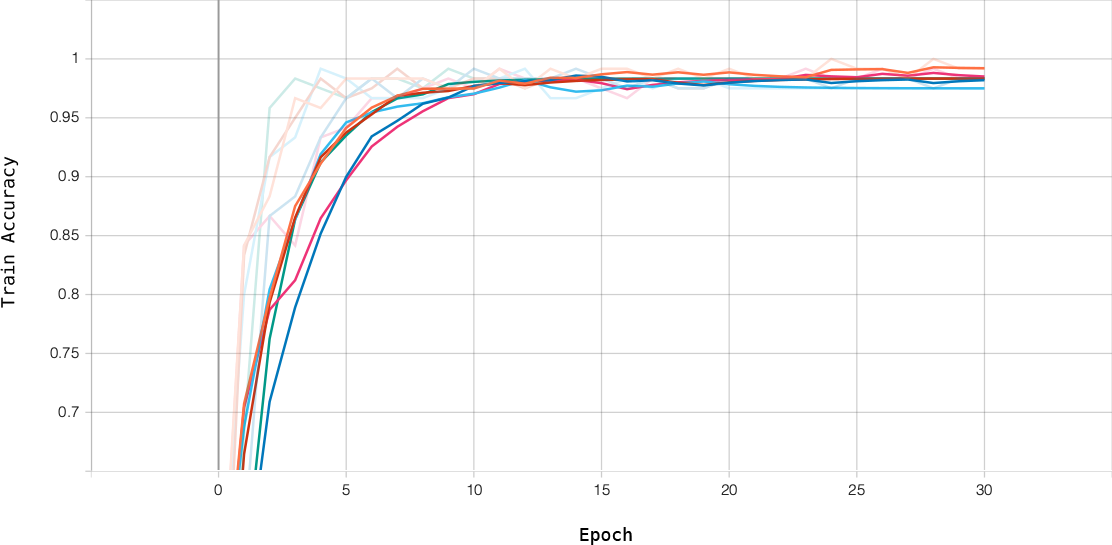
\includegraphics[width=\textwidth]{bhh_case_study/iris/train_accuracy.png}
		\caption{Train accuracy}
		\label{fig:results:case_study:iris:train:accuracy}
	\end{subfigure}
	\begin{subfigure}{0.49\textwidth}
		\centering
		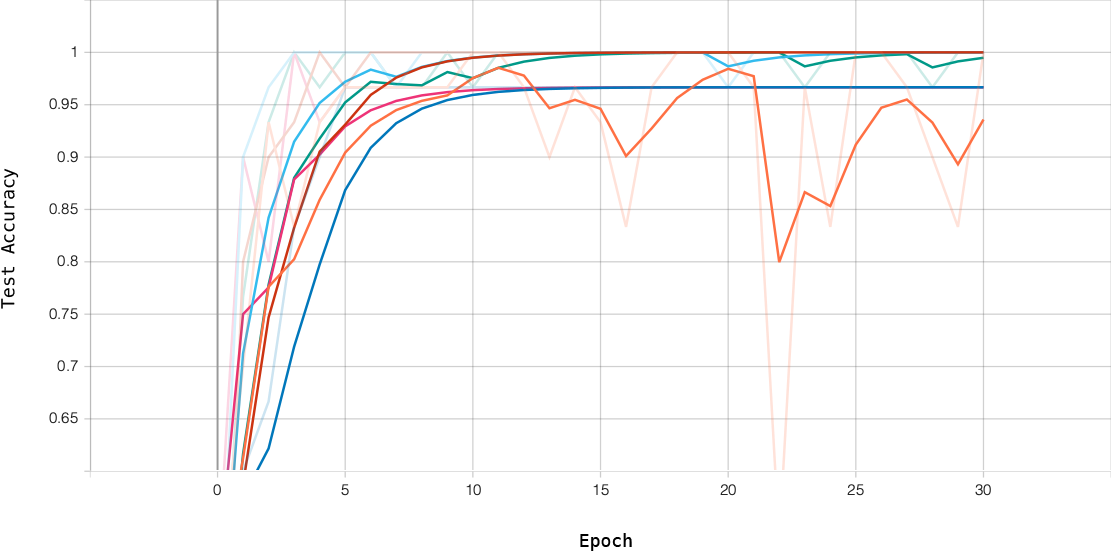
\includegraphics[width=\textwidth]{bhh_case_study/iris/test_accuracy.png}
		\caption{Test accuracy}
		\label{fig:results:case_study:iris:test:accuracy}
	\end{subfigure}
	\par\bigskip
	\begin{subfigure}{\textwidth}
		\centering
		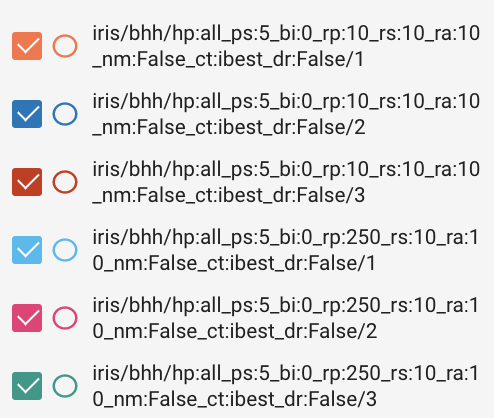
\includegraphics[width=0.35\textwidth]{bhh_case_study/iris/legend.png}
		\caption{Legend}
		\label{fig:results:case_study:iris:legend}
	\end{subfigure}
	\par\bigskip
	\caption{Train and test behaviour of the \Ac{BHH} baseline for different configurations of replay window size}
	\label{fig:results:case_study:iris:metric_plots}
\end{figure}

A high level view of the train and test metric plots is good for drawing high level conclusions, but more detail is required. Figure \ref{fig:results:case_study:iris:alpha} aims to provide more detail as to what is happening during training and plots the value of $\alpha$ during training. Each sub-figure represents the value of $\alpha$ for a particular index, representing a particular \index{heuristic}heuristic. From sub-figures \ref{fig:results:case_study:iris:alpha:0}, \ref{fig:results:case_study:iris:alpha:2} and \ref{fig:results:case_study:iris:alpha:6}, the effect of a larger replay value is clear. Although a more detailed discussed on replay window sizes is left for Section \ref{sec:results:replay}, one can clearly see the accumulation of ``knowledge''/``evidence'' in the concentration parameter $\alpha$. It should be noticeable then from these sub-figures how $\alpha$ changes over time for runs with lower replay window sizes and is indicative of the learning capabilities of the \Ac{BHH}.  From these changes, one can formulate a prediction of which \index{heuristic}heuristics are then likely to be selected in the next steps.

Figures \ref{fig:results:case_study:iris:alpha:5} and \ref{fig:results:case_study:iris:alpha:9} contain a run in orange that shows how the concentration for a particular heuristic (\Acs{Adadelta} and \Acs{DE}) and can change over time. This suggests that the \Acs{BHH} has the ability to dynamically switch between heuristics as the need requires. This concept bears similarities to dynamic optimisation algorithms. It can thus be said that an observation is made that the \Acs{BHH} is able to learn (to some degree) to balance exploration and exploitation by dynamically changing the heuristic of interest at that point in time. Notice that it has not yet been established if the attempt to balance leads to good or bad outcomes. However, this is a still a useful feature of the \Acs{BHH} and warrants further discussion and reasoning. These statements further support the hypothesis that there might not be a no single specific heuristic that is the best heuristic to train the \Acs{FFNN} during the entire training process. In the succeeding sections, it is shown how this statement is further supported as the behaviour of the \Acs{BHH} is shown to be problem-dependent.

A clear distinction between Figures \ref{fig:results:case_study:iris:metric_plots} and \ref{fig:results:case_study:iris:alpha} should be pointed out. Figures \ref{fig:results:case_study:iris:metric_plots} plot metrics for every epoch, while Figure \ref{fig:results:case_study:iris:alpha} plot metrics for every mini-batch iteration. This is a subtle difference in visualisation, but nonetheless important. A more fine-grained visualisation illustrates the learning opportunities better since it is clear that a single step of learning happens on a single mini-batch iteration. This is important to keep in mind for various different sizes of datasets.


\begin{figure}[htbp]
	\begin{subfigure}{0.5\textwidth}
		\centering
		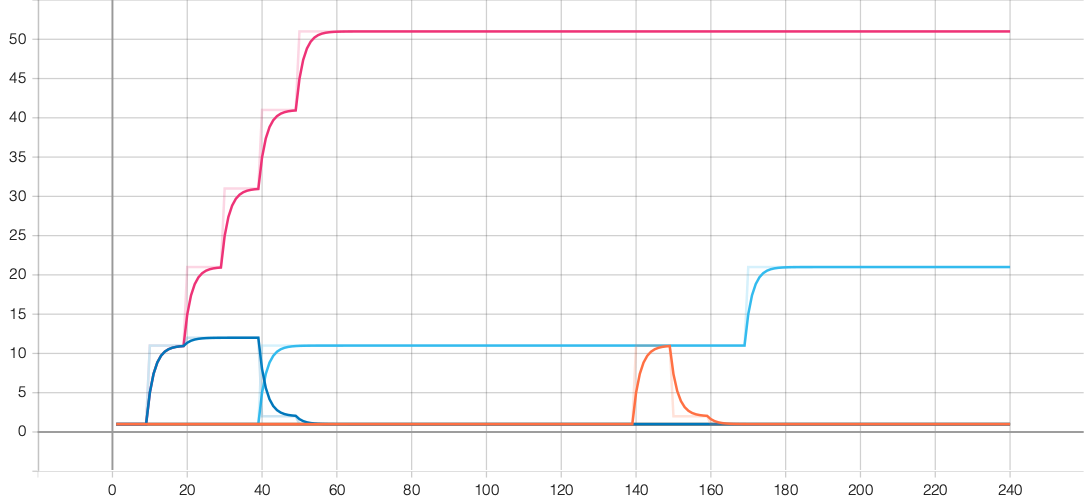
\includegraphics[width=\textwidth]{bhh_case_study/iris/alpha[0].png}
		\caption{$\alpha_{0}$ - \Acs{SGD}}
		\label{fig:results:case_study:iris:alpha:0}
	\end{subfigure}
	\begin{subfigure}{0.5\textwidth}
		\centering
		\includegraphics[width=\textwidth]{bhh_case_study/iris/alpha[1].png}
		\caption{$\alpha_{1}$ - \Acs{Momentum}}
		\label{fig:results:case_study:iris:alpha:1}
	\end{subfigure}
	\par\bigskip
	\begin{subfigure}{0.5\textwidth}
		\centering
		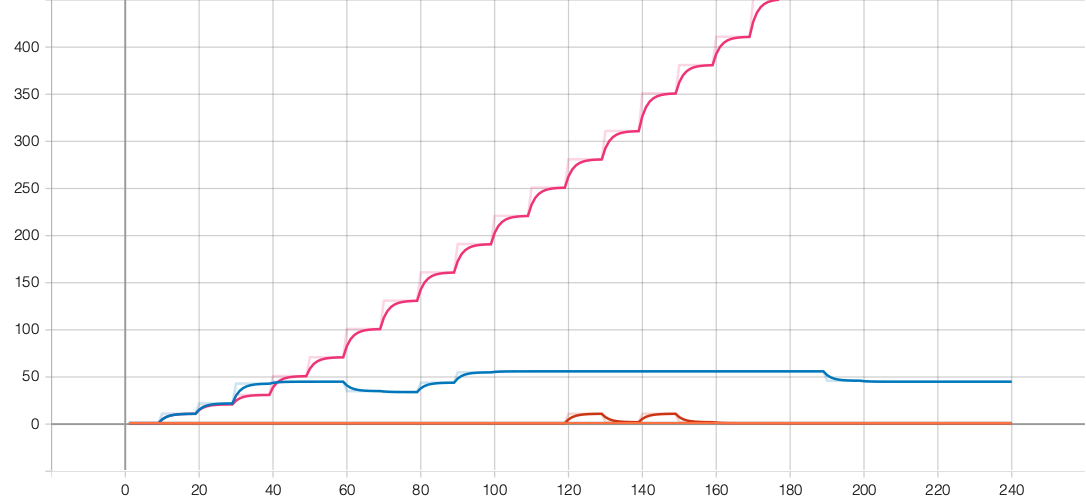
\includegraphics[width=\textwidth]{bhh_case_study/iris/alpha[2].png}
		\caption{$\alpha_{2}$ - \Acs{NAG}}
		\label{fig:results:case_study:iris:alpha:2}
	\end{subfigure}
	\begin{subfigure}{0.5\textwidth}
		\centering
		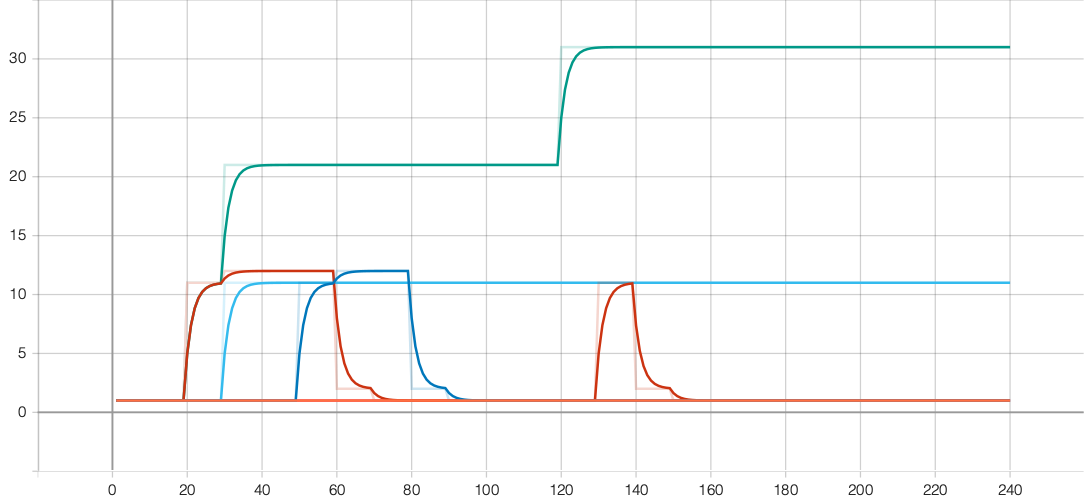
\includegraphics[width=\textwidth]{bhh_case_study/iris/alpha[3].png}
		\caption{$\alpha_{3}$ - \Acs{Adagrad}}
		\label{fig:results:case_study:iris:alpha:3}
	\end{subfigure}
	\par\bigskip
	\begin{subfigure}{0.5\textwidth}
		\centering
		\includegraphics[width=\textwidth]{bhh_case_study/iris/alpha[4].png}
		\caption{$\alpha_{4}$ - \Acs{RMSProp}}
		\label{fig:results:case_study:iris:alpha:4}
	\end{subfigure}
	\begin{subfigure}{0.5\textwidth}
		\centering
		\includegraphics[width=\textwidth]{bhh_case_study/iris/alpha[5].png}
		\caption{$\alpha_{5}$ - \Acs{Adadelta}}
		\label{fig:results:case_study:iris:alpha:5}
	\end{subfigure}
	\par\bigskip
	\begin{subfigure}{0.5\textwidth}
		\centering
		\includegraphics[width=\textwidth]{bhh_case_study/iris/alpha[6].png}
		\caption{$\alpha_{6}$ - \Acs{Adam}}
		\label{fig:results:case_study:iris:alpha:6}
	\end{subfigure}
	\begin{subfigure}{0.5\textwidth}
		\centering
		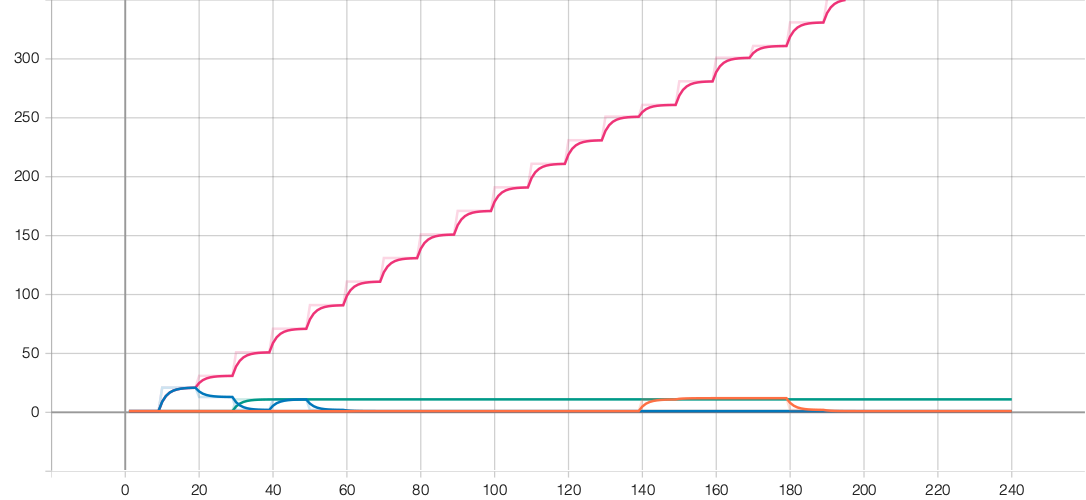
\includegraphics[width=\textwidth]{bhh_case_study/iris/alpha[7].png}
		\caption{$\alpha_{7}$ - \Acs{PSO}}
		\label{fig:results:case_study:iris:alpha:7}
	\end{subfigure}
	\par\bigskip
	\begin{subfigure}{0.5\textwidth}
		\centering
		\includegraphics[width=\textwidth]{bhh_case_study/iris/alpha[8].png}
		\caption{$\alpha_{8}$ - \Acs{GA}}
		\label{fig:results:case_study:iris:alpha:8}
	\end{subfigure}
	\begin{subfigure}{0.5\textwidth}
		\centering
		\includegraphics[width=\textwidth]{bhh_case_study/iris/alpha[9].png}
		\caption{$\alpha_{9}$ - \Acs{DE}}
		\label{fig:results:case_study:iris:alpha:9}
	\end{subfigure}
	\par\bigskip
	\caption{Change in the concentration of $\alpha$ during training for various heuristics}
	\label{fig:results:case_study:iris:alpha}
\end{figure}

Due to the Bayesian nature of the \Acs{BHH}, one can expect the plots from figure \ref{fig:results:case_study:iris:alpha} to drive the plots presented in \ref{fig:results:case_study:iris:p_theta} as these two parameters are related. The parameter $\alpha$ is the concentration parameter for the Dirichlet probability distribution represented by $\theta$. The reader is now urged to consider Figures \ref{fig:results:case_study:iris:alpha:6} and \ref{fig:results:case_study:iris:p_theta:6} together. These two figures illustrate the above mentioned Bayesian concepts well. It should be noted that as $\alpha$ changes, $\theta$ will change. More specifically, the longer the ``memory'' of the \Acs{BHH} the greater the magnitude of $\alpha$ resulting in a sampled selection probability $\theta$ that converges to the ``learnt'' expected selection probability ($E\left[\theta\right]$). The impact of this concept (retained memory) is addressed in Sections \ref{sec:results:replay}.

\begin{figure}[htbp]
	\begin{subfigure}{0.5\textwidth}
		\centering
		\includegraphics[width=\textwidth]{bhh_case_study/iris/theta[0].png}
		\caption{$P(\theta_{0} | \alpha)$ - \Acs{SGD}}
		\label{fig:results:case_study:iris:p_theta:0}
	\end{subfigure}
	\begin{subfigure}{0.5\textwidth}
		\centering
		\includegraphics[width=\textwidth]{bhh_case_study/iris/theta[1].png}
		\caption{$P(\theta_{1} | \alpha)$ - \Acs{Momentum}}
		\label{fig:results:case_study:iris:p_theta:1}
	\end{subfigure}
	\par\medskip
	\begin{subfigure}{0.5\textwidth}
		\centering
		\includegraphics[width=\textwidth]{bhh_case_study/iris/theta[2].png}
		\caption{$P(\theta_{2} | \alpha)$ - \Acs{NAG}}
		\label{fig:results:case_study:iris:p_theta:2}
	\end{subfigure}
	\begin{subfigure}{0.5\textwidth}
		\centering
		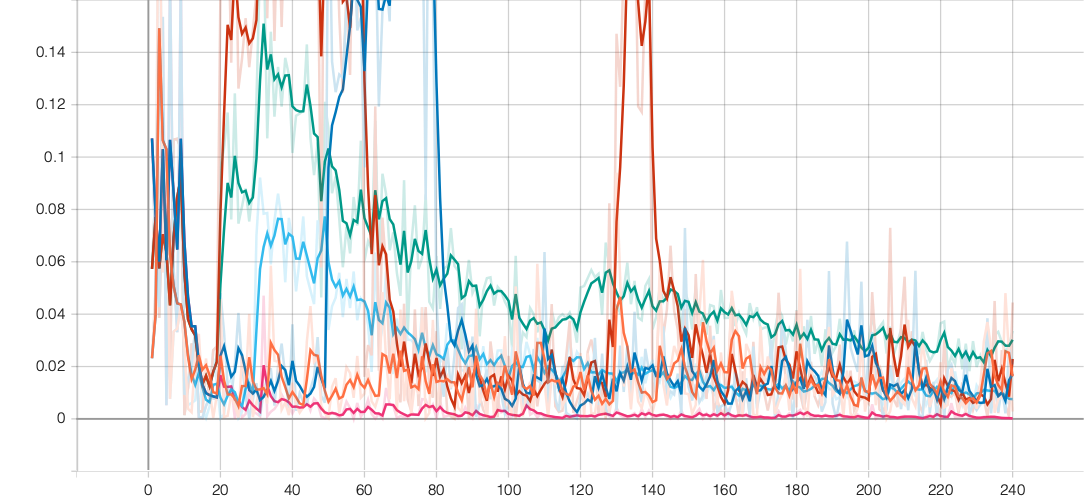
\includegraphics[width=\textwidth]{bhh_case_study/iris/theta[3].png}
		\caption{$P(\theta_{3} | \alpha)$ - \Acs{Adagrad}}
		\label{fig:results:case_study:iris:p_theta:3}
	\end{subfigure}
	\par\medskip
	\begin{subfigure}{0.5\textwidth}
		\centering
		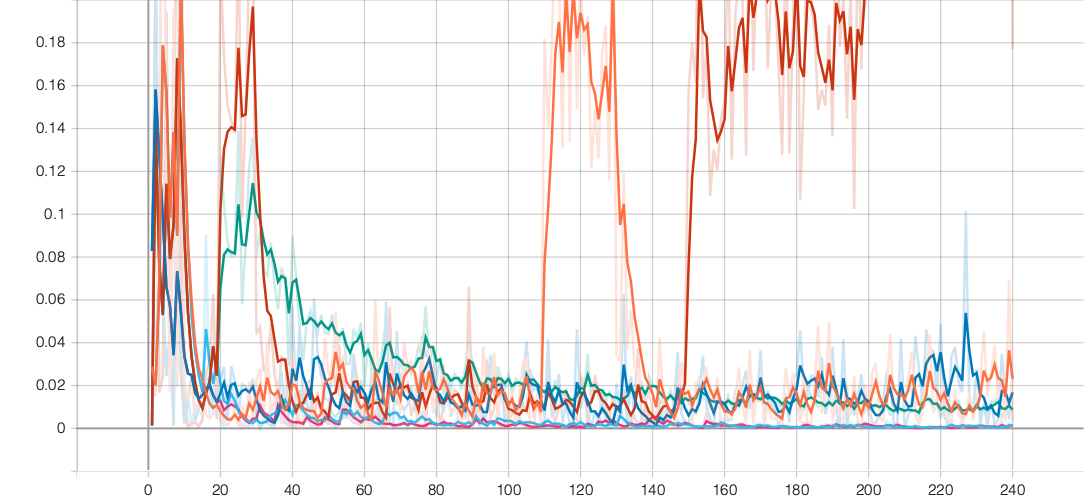
\includegraphics[width=\textwidth]{bhh_case_study/iris/theta[4].png}
		\caption{$P(\theta_{4} | \alpha)$ - \Acs{RMSProp}}
		\label{fig:results:case_study:iris:p_theta:4}
	\end{subfigure}
	\begin{subfigure}{0.5\textwidth}
		\centering
		\includegraphics[width=\textwidth]{bhh_case_study/iris/theta[5].png}
		\caption{$P(\theta_{5} | \alpha)$ - \Acs{Adadelta}}
		\label{fig:results:case_study:iris:p_theta:5}
	\end{subfigure}
	\par\medskip
	\begin{subfigure}{0.5\textwidth}
		\centering
		\includegraphics[width=\textwidth]{bhh_case_study/iris/theta[6].png}
		\caption{$P(\theta_{6} | \alpha)$ - \Acs{Adam}}
		\label{fig:results:case_study:iris:p_theta:6}
	\end{subfigure}
	\begin{subfigure}{0.5\textwidth}
		\centering
		\includegraphics[width=\textwidth]{bhh_case_study/iris/theta[7].png}
		\caption{$P(\theta_{7} | \alpha)$ - \Acs{PSO}}
		\label{fig:results:case_study:iris:p_theta:7}
	\end{subfigure}
	\par\medskip
	\begin{subfigure}{0.5\textwidth}
		\centering
		\includegraphics[width=\textwidth]{bhh_case_study/iris/theta[8].png}
		\caption{$P(\theta_{8} | \alpha)$ - \Acs{GA}}
		\label{fig:results:case_study:iris:p_theta:8}
	\end{subfigure}
	\begin{subfigure}{0.5\textwidth}
		\centering
		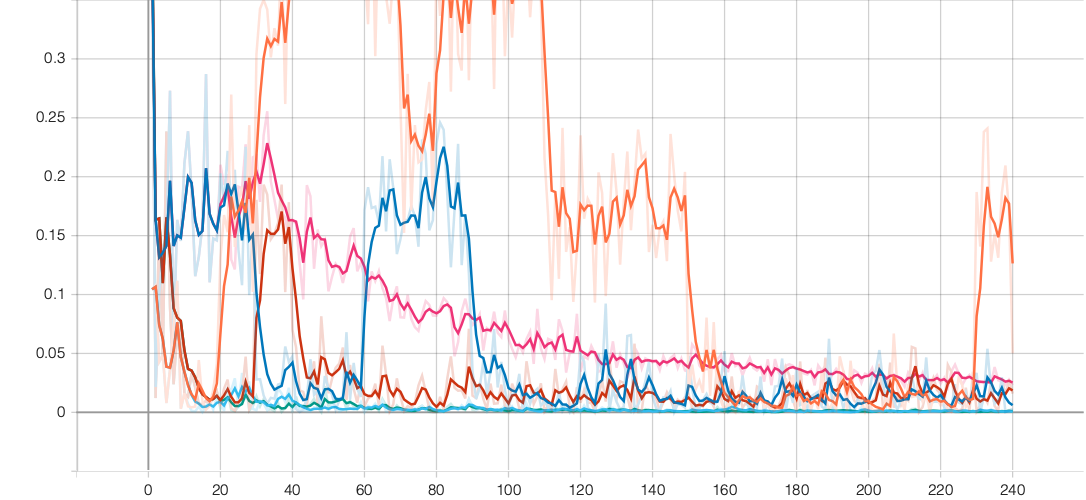
\includegraphics[width=\textwidth]{bhh_case_study/iris/theta[9].png}
		\caption{$P(\theta_{9} | \alpha)$ - \Acs{DE}}
		\label{fig:results:case_study:iris:p_theta:9}
	\end{subfigure}
	\par\medskip
	\caption{Change in the sampled selection probability of $\theta$ during training for various heuristics}
	\label{fig:results:case_study:iris:p_theta}
\end{figure}








Another observation that can be made from Figures \ref{fig:results:case_study:iris:alpha} and \ref{fig:results:case_study:iris:p_theta} is that none of the runs are the same. This is of course due to the stochastic nature of the \Acs{BHH} and the noise caused by using mini-batches. However, it highlights the fact that the learning process for the \Acs{BHH} has to be adaptive from run to run. This is evident in the plots presented in Figure \ref{fig:results:case_study:iris:p_H} as one can see how the \index{heuristic}heuristic selection probability changes over time. This is proof that the \Ac{BHH} is learning something, but it is yet to be established what exactly it is learning. It is said that the \Acs{BHH} updates its \textit{beliefs} (prior knowledge) about which heuristic to select by biasing selection towards \index{heuristic}heuristic performance. It can therefore be concluded that any learning that is done, is done as a result of learning from performance. Since the performance criteria mechanism for the \Ac{BHH}, called the \textit{credit assignment strategy} marks a successful event as one meeting the performance criteria. Although this event is very much a local event, the continuous application of it over all runs means that learning does account for positive learning towards the overall performance goals.




\begin{figure}[htbp]
	\begin{subfigure}{0.5\textwidth}
		\centering
		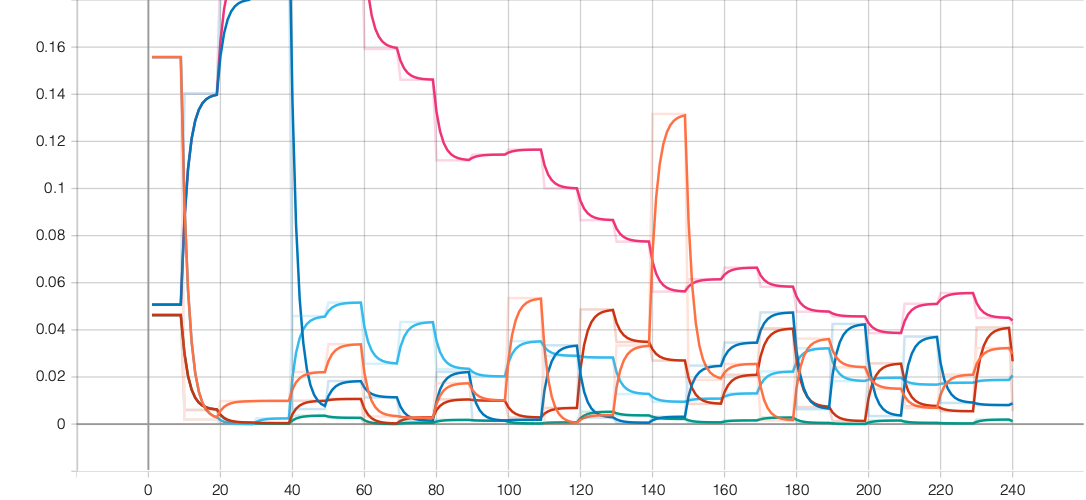
\includegraphics[width=\textwidth]{bhh_case_study/iris/p_H[0].png}
		\caption{$P\left(h_{0} | \theta \right)$ - \Acs{SGD}}
		\label{fig:results:case_study:iris:p_H:0}
	\end{subfigure}
	\begin{subfigure}{0.5\textwidth}
		\centering
		\includegraphics[width=\textwidth]{bhh_case_study/iris/p_H[1].png}
		\caption{$P\left(h_{1} | \theta \right)$ - \Acs{Momentum}}
		\label{fig:results:case_study:iris:p_H:1}
	\end{subfigure}
	\par\medskip
	\begin{subfigure}{0.5\textwidth}
		\centering
		\includegraphics[width=\textwidth]{bhh_case_study/iris/p_H[2].png}
		\caption{$P\left(h_{2} | \theta \right)$ - \Acs{NAG}}
		\label{fig:results:case_study:iris:p_H:2}
	\end{subfigure}
	\begin{subfigure}{0.5\textwidth}
		\centering
		\includegraphics[width=\textwidth]{bhh_case_study/iris/p_H[3].png}
		\caption{$P\left(h_{3} | \theta \right)$ - \Acs{Adagrad}}
		\label{fig:results:case_study:iris:p_H:3}
	\end{subfigure}
	\par\medskip
	\begin{subfigure}{0.5\textwidth}
		\centering
		\includegraphics[width=\textwidth]{bhh_case_study/iris/p_H[4].png}
		\caption{$P\left(h_{4} | \theta \right)$ - \Acs{RMSProp}}
		\label{fig:results:case_study:iris:p_H:4}
	\end{subfigure}
	\begin{subfigure}{0.5\textwidth}
		\centering
		\includegraphics[width=\textwidth]{bhh_case_study/iris/p_H[5].png}
		\caption{$P\left(h_{5} | \theta \right)$ - \Acs{Adadelta}}
		\label{fig:results:case_study:iris:p_H:5}
	\end{subfigure}
	\par\medskip
	\begin{subfigure}{0.5\textwidth}
		\centering
		\includegraphics[width=\textwidth]{bhh_case_study/iris/p_H[6].png}
		\caption{$P\left(h_{6} | \theta \right)$ - \Acs{Adam}}
		\label{fig:results:case_study:iris:p_H:6}
	\end{subfigure}
	\begin{subfigure}{0.5\textwidth}
		\centering
		\includegraphics[width=\textwidth]{bhh_case_study/iris/p_H[7].png}
		\caption{$P\left(h_{7} | \theta \right)$ - \Acs{PSO}}
		\label{fig:results:case_study:iris:p_H:7}
	\end{subfigure}
	\par\medskip
	\begin{subfigure}{0.5\textwidth}
		\centering
		\includegraphics[width=\textwidth]{bhh_case_study/iris/p_H[8].png}
		\caption{$P\left(h_{8} | \theta \right)$ - \Acs{GA}}
		\label{fig:results:case_study:iris:p_H:8}
	\end{subfigure}
	\begin{subfigure}{0.5\textwidth}
		\centering
		\includegraphics[width=\textwidth]{bhh_case_study/iris/p_H[9].png}
		\caption{$P\left(h_{9} | \theta \right)$ - \Acs{DE}}
		\label{fig:results:case_study:iris:p_H:9}
	\end{subfigure}
	\par\medskip
	\caption{Change in the prior heuristic selection probability $P\left(H\right | \theta )$ as the \Ac{BHH} learns during training}
	\label{fig:results:case_study:iris:p_H}
\end{figure}


Consider now Figure \ref{fig:results:case_study:iris:p_theta:6} again, but this time include a configuration of the \Acs{BHH} where no \index{Bayesian Analysis}Bayesian Analysis takes place, resulting in a purely random \index{heuristic}heuristic selection probability throughout. Such an configuration is given in Figure \ref{fig:results:case_study:iris:no_learn:metrics} below for the sampled \index{heuristic}heuristic selection probability for \Acs{Adam} (gray).

\begin{figure}[htbp]
	\begin{subfigure}{0.5\textwidth}
		\centering
		\includegraphics[width=\textwidth]{bhh_case_study/iris/no_learning_theta.png}
		\caption{$P(\theta_{6} | \alpha)$}
		\label{fig:results:case_study:iris:no_learn:p_theta}
	\end{subfigure}
	\begin{subfigure}{0.5\textwidth}
		\centering
		\includegraphics[width=\textwidth]{bhh_case_study/iris/no_learning_test_loss.png}
		\caption{Test loss}
		\label{fig:results:case_study:iris:no_learn:test:loss}
	\end{subfigure}
	\par\bigskip
	\caption{Comparing baseline \Acp{BHH} to that of a \Ac{BHH} with pure random selection.}
	\label{fig:results:case_study:iris:no_learn:metrics}
\end{figure}

One can see that the random configuration (gray) illustrated almost a fixed pattern behaviour, from which we can draw the following conclusions:

\begin{itemize}
	\item Despite a completely random heuristic selection probability, the underlying \Acs{BHH} was still able to learn and perform relatively well. If the ability to learn is then purely based on the \textit{perturbative} components of the \Acs{BHH} it can be concluded that the proxied heuristic step operations are successful.

	\item This shows that the \Acs{BHH} selection mechanism is indeed facilitating a learning process and since \Acs{Adam} is known to perform well on the iris dataset, it can be concluded that the learning process is successful and beneficial to the outcome of the \Acs{BHH}.
\end{itemize}

The statements made above conclude the successful working of the \Acs{BHH}. Both the perturbative element (through proxied heuristic update steps) and the selection mechanism (through Bayesian analysis) is shown to work successfully. Figure \ref{fig:results:case_study:iris:p_HgEC} shows the resulting output of the predictive model for each of the five entities in the heuristic pool. This predicted heuristic selection probability is used to parameterise a new categorical distribution from which the heuristics are finally sampled and (re)selected.

\begin{figure}[htbp]
	\begin{subfigure}{0.5\textwidth}
		\centering
		\includegraphics[width=\textwidth]{bhh_case_study/iris/p_HgEC[0][6].png}
		\caption{$P\left(h_{6}|e_{0},c_{1}\right)$ - entity 0 + \Acs{Adam} }
		\label{fig:results:case_study:iris:p_HgEC:0:6}
	\end{subfigure}
	\begin{subfigure}{0.5\textwidth}
		\centering
		\includegraphics[width=\textwidth]{bhh_case_study/iris/p_HgEC[1][6].png}
		\caption{$P\left(h_{6}|e_{1},c_{1}\right)$ - entity 1 + \Acs{Adam} }
		\label{fig:results:case_study:iris:p_HgEC:1:6}
	\end{subfigure}
	\par\bigskip
	\begin{subfigure}{0.5\textwidth}
		\centering
		\includegraphics[width=\textwidth]{bhh_case_study/iris/p_HgEC[2][6].png}
		\caption{$P\left(h_{6}|e_{2},c_{1}\right)$ - entity 2 + \Acs{Adam} }
		\label{fig:results:case_study:iris:p_HgEC:2:6}
	\end{subfigure}
	\begin{subfigure}{0.5\textwidth}
		\centering
		\includegraphics[width=\textwidth]{bhh_case_study/iris/p_HgEC[3][6].png}
		\caption{$P\left(h_{6}|e_{3},c_{1}\right)$ - entity 3 + \Acs{Adam} }
		\label{fig:results:case_study:iris:p_HgEC:3:6}
	\end{subfigure}
	\par\bigskip
	\begin{subfigure}{\textwidth}
		\centering
		\includegraphics[width=0.5\textwidth]{bhh_case_study/iris/p_HgEC[4][6].png}
		\caption{$P\left(h_{6}|e_{4},c_{1}\right)$ - entity 4 + \Acs{Adam} }
		\label{fig:results:case_study:iris:p_HgEC:4:6}
	\end{subfigure}
	\par\bigskip
	\caption{Change in the realised output of the predictive model $P\left(H|E,C;\theta,\phi,\psi \right)$ showcasing the selection of the \Acs{Adam} optimiser/low-level heuristic as an example}
	\label{fig:results:case_study:iris:p_HgEC}
\end{figure}

Figure \ref{fig:results:case_study:iris:HgEC} show the resulting selected \index{heuristic}heuristic, per entity, over time. From these plots, one can see how convergence on \Acs{Adam} occurs at least at some point during training for the majority of the entities.


\begin{figure}[htbp]
	\begin{subfigure}{0.5\textwidth}
		\centering
		\includegraphics[width=\textwidth]{bhh_case_study/iris/HgEC[0].png}
		\caption{HgEC\lbrack0\rbrack - entity 0}
		\label{fig:results:case_study:iris:HgEC:0}
	\end{subfigure}
	\begin{subfigure}{0.5\textwidth}
		\centering
		\includegraphics[width=\textwidth]{bhh_case_study/iris/HgEC[1].png}
		\caption{HgEC\lbrack1\rbrack - entity 1}
		\label{fig:results:case_study:iris:HgEC:1}
	\end{subfigure}
	\par\bigskip
	\begin{subfigure}{0.5\textwidth}
		\centering
		\includegraphics[width=\textwidth]{bhh_case_study/iris/HgEC[2].png}
		\caption{HgEC\lbrack2\rbrack - entity 2}
		\label{fig:results:case_study:iris:HgEC:2}
	\end{subfigure}
	\begin{subfigure}{0.5\textwidth}
		\centering
		\includegraphics[width=\textwidth]{bhh_case_study/iris/HgEC[3].png}
		\caption{HgEC\lbrack3\rbrack - entity 3}
		\label{fig:results:case_study:iris:HgEC:3}
	\end{subfigure}
	\par\bigskip
	\begin{subfigure}{\textwidth}
		\centering
		\includegraphics[width=0.5\textwidth]{bhh_case_study/iris/HgEC[4].png}
		\caption{HgEC\lbrack4\rbrack - entity 4}
		\label{fig:results:case_study:iris:HgEC:4}
	\end{subfigure}
	\par\bigskip
	\caption{Change in selected heuristics (HgEC) during training for various entities}
	\label{fig:results:case_study:iris:HgEC}
\end{figure}

Finally, Figure \ref{fig:results:case_study:iris:adam:HgEC} below shows all of the probabilistic components involved in the selection mechanism of the \Ac{BHH}.

\begin{figure}[htbp]
	\begin{subfigure}{0.5\textwidth}
		\centering
		\includegraphics[width=\textwidth]{bhh_case_study/iris/alpha[6].png}
		\caption{$\alpha_{6}$ - \Acs{Adam}}
		\label{fig:results:case_study:iris:adam:alpha:6}
	\end{subfigure}
	\begin{subfigure}{0.5\textwidth}
		\centering
		\includegraphics[width=\textwidth]{bhh_case_study/iris/theta[6].png}
		\caption{$P(\theta_{6} | \alpha)$ - \Acs{Adam}}
		\label{fig:results:case_study:iris:adam:p_theta:6}
	\end{subfigure}
	\par\bigskip
	\begin{subfigure}{0.5\textwidth}
		\centering
		\includegraphics[width=\textwidth]{bhh_case_study/iris/p_H[6].png}
		\caption{$P\left(h_{6} | \theta \right)$ - \Acs{Adam}}
		\label{fig:results:case_study:iris:adam:p_H:6}
	\end{subfigure}
	\begin{subfigure}{0.5\textwidth}
		\centering
		\includegraphics[width=\textwidth]{bhh_case_study/iris/p_HgEC[1][6].png}
		\caption{$P\left(h_{6}|e_{1},c_{1}\right)$ - entity 1 + \Acs{Adam} }
		\label{fig:results:case_study:iris:adam:p_HgEC:1:6}
	\end{subfigure}
	\par\bigskip
	\begin{subfigure}{\textwidth}
		\centering
		\includegraphics[width=0.5\textwidth]{bhh_case_study/iris/HgEC[1].png}
		\caption{HgEC\lbrack1\rbrack - entity 1}
		\label{fig:results:case_study:iris:adam:HgEC:1}
	\end{subfigure}
	\par\bigskip
	\caption{An illustration that shows the effects of learning as for \Acs{Adam}}
	\label{fig:results:case_study:iris:adam:HgEC}
\end{figure}


The behaviour of the \Ac{BHH} has been studied and it is found to be successful in its intent to learn which \index{heuristic}heuristics to use throughout the training process. It has also been shown that the training of the \acp{FFNN} with \Acp{BHH} is done by means of a \index{heuristic}heuristic selection mechanism and proxied \index{heuristic}heuristic update steps, both which have been shown to attribute to the successful training of the \acp{FFNN}.

Although these observations are good, these are still high level and not based on any statistical data. It is purely based on observation over a few runs. The following section aims to provide the first set of conclusions based on a statistically certain comparison of the \Ac{BHH}'s performance to that of standalone low-level \index{heuristic}heuristics.


\section{Standalone vs BHH Baseline}
\label{sec:results:standalone}

This section provides the empirical results of the experiment group that compare the performance of the \Ac{BHH} to that of well-known, standalone, low-level heuristics. Table \ref{tab:results:standalone:metrics} below shows the count, average and standard deviation of the ranks achieved by die various heuristics for all timestamps, across all datasets. Furthermore, the table orders the \index{heuristic}heuristics by a normalised overall rank.

\begin{table}[htbp]
	\centering
	\caption{Empirical results showcasing rank statistics for different standalone \index{heuristic}heuristics compared to the baseline \acs{BHH} across multiple datasets}
	\label{tab:results:standalone:metrics}%
	\par\bigskip
	\resizebox{\textwidth}{!}{
		\begin{tabular}{rcccccccccccc}
			\textbf{step}                      & \multicolumn{1}{l}{\textbf{(All)}}     &                                                                                    &                                                                           &                                                                           &                                                                           &                                               &                                             &                                                &                                                &                                                &                                                &                                                \\
			\cmidrule{1-2}                     &                                        &                                                                                    &                                                                           &                                                                           &                                                                           &                                               &                                             &                                                &                                                &                                                &                                                &                                                \\
			                                   &                                        & \multicolumn{1}{l}{\textbf{heuristic}}                                             &                                                                           &                                                                           &                                                                           &                                               &                                             &                                                &                                                &                                                &                                                &                                                \\
			\cmidrule{3-3}    \textbf{dataset} & \multicolumn{1}{l}{\textbf{statistic}} & \textbf{adagrad}                                                                   & \textbf{adam}                                                             & \textbf{nag}                                                              & \textbf{rmsprop}                                                          & \textbf{bhh}                                  & \textbf{adadelta}                           & \textbf{ga}                                    & \textbf{sgd}                                   & \textbf{pso}                                   & \textbf{momentum}                              & \textbf{de}                                    \\
			\midrule
			abalone                            & count                                  & 930                                                                                & 930                                                                       & 930                                                                       & 930                                                                       & 930                                           & 930                                         & 930                                            & 930                                            & 930                                            & 930                                            & 930                                            \\
			                                   & avg                                    & \cellcolor[rgb]{ .776,  .937,  .808}\textcolor[rgb]{ 0,  .38,  0}{2.0323}          & 2.2086                                                                    & 3.8108                                                                    & 4.0849                                                                    & 5.1430                                        & 4.7151                                      & 9.1839                                         & 6.9043                                         & 9.3914                                         & 7.9441                                         & 10.5817                                        \\
			                                   & std                                    & 1.3436                                                                             & 1.5671                                                                    & 1.2760                                                                    & 2.2093                                                                    & 1.9327                                        & 1.1671                                      & 0.9030                                         & 0.7740                                         & 1.5268                                         & 0.9717                                         & 1.1291                                         \\
			adult                              & count                                  & 930                                                                                & 930                                                                       & 930                                                                       & 930                                                                       & 930                                           & 930                                         & 930                                            & 930                                            & 930                                            & 930                                            & 930                                            \\
			                                   & avg                                    & 5.1570                                                                             & 6.3559                                                                    & \cellcolor[rgb]{ .776,  .937,  .808}\textcolor[rgb]{ 0,  .38,  0}{1.4914} & 5.6968                                                                    & 10.1710                                       & 2.4720                                      & 7.7688                                         & 2.8237                                         & 9.6043                                         & 3.6688                                         & 9.0140                                         \\
			                                   & std                                    & 1.2838                                                                             & 1.4823                                                                    & 0.6870                                                                    & 1.4006                                                                    & 2.2688                                        & 1.2974                                      & 1.3461                                         & 1.1988                                         & 1.6718                                         & 1.3834                                         & 1.5614                                         \\
			air\_quality                       & count                                  & 930                                                                                & 930                                                                       & 930                                                                       & 930                                                                       & 930                                           & 930                                         & 930                                            & 930                                            & 930                                            & 930                                            & 930                                            \\
			                                   & avg                                    & 3.0688                                                                             & 4.4849                                                                    & 3.2527                                                                    & \cellcolor[rgb]{ .776,  .937,  .808}\textcolor[rgb]{ 0,  .38,  0}{2.9269} & 5.4989                                        & 4.4204                                      & 6.3785                                         & 8.7548                                         & 8.1151                                         & 9.8301                                         & 9.2688                                         \\
			                                   & std                                    & 1.8148                                                                             & 2.0087                                                                    & 1.7266                                                                    & 2.0466                                                                    & 2.5018                                        & 2.5575                                      & 1.7707                                         & 1.4074                                         & 1.9775                                         & 1.3046                                         & 1.9578                                         \\
			bank                               & count                                  & 930                                                                                & 930                                                                       & 930                                                                       & 930                                                                       & 930                                           & 930                                         & 930                                            & 930                                            & 930                                            & 930                                            & 930                                            \\
			                                   & avg                                    & 2.4161                                                                             & \cellcolor[rgb]{ .776,  .937,  .808}\textcolor[rgb]{ 0,  .38,  0}{1.9882} & 3.8516                                                                    & 3.1591                                                                    & 5.4688                                        & 5.0108                                      & 9.0505                                         & 7.2301                                         & 9.9043                                         & 7.3892                                         & 10.5312                                        \\
			                                   & std                                    & 1.3873                                                                             & 1.3985                                                                    & 1.4056                                                                    & 1.8653                                                                    & 1.7489                                        & 0.9864                                      & 0.9955                                         & 0.9144                                         & 1.2374                                         & 0.8907                                         & 1.0445                                         \\
			bike                               & count                                  & 930                                                                                & 930                                                                       & 930                                                                       & 930                                                                       & 930                                           & 930                                         & 930                                            & 930                                            & 930                                            & 930                                            & 930                                            \\
			                                   & avg                                    & \cellcolor[rgb]{ .776,  .937,  .808}\textcolor[rgb]{ 0,  .38,  0}{1.6710}          & 3.2559                                                                    & 5.4247                                                                    & 5.4140                                                                    & 3.5903                                        & 4.3774                                      & 7.2591                                         & 8.3656                                         & 7.4000                                         & 8.7441                                         & 10.4978                                        \\
			                                   & std                                    & 1.1854                                                                             & 3.2580                                                                    & 0.9310                                                                    & 3.7231                                                                    & 1.0534                                        & 1.0684                                      & 1.0992                                         & 1.3163                                         & 1.6037                                         & 1.2745                                         & 1.2717                                         \\
			car                                & count                                  & 930                                                                                & 930                                                                       & 930                                                                       & 930                                                                       & 930                                           & 930                                         & 930                                            & 930                                            & 930                                            & 930                                            & 930                                            \\
			                                   & avg                                    & 3.8591                                                                             & \cellcolor[rgb]{ .776,  .937,  .808}\textcolor[rgb]{ 0,  .38,  0}{1.5022} & 5.0839                                                                    & 2.0946                                                                    & 2.9720                                        & 6.5903                                      & 8.9301                                         & 8.4108                                         & 7.0118                                         & 9.0731                                         & 10.4720                                        \\
			                                   & std                                    & 0.8054                                                                             & 1.1602                                                                    & 0.6925                                                                    & 1.1095                                                                    & 1.0151                                        & 1.4439                                      & 1.2877                                         & 1.2333                                         & 1.2970                                         & 1.1743                                         & 1.2916                                         \\
			diabetic                           & count                                  & 930                                                                                & 930                                                                       & 930                                                                       & 930                                                                       & 930                                           & 930                                         & 930                                            & 930                                            & 930                                            & 930                                            & 930                                            \\
			                                   & avg                                    & 2.6129                                                                             & 6.0634                                                                    & \cellcolor[rgb]{ .776,  .937,  .808}\textcolor[rgb]{ 0,  .38,  0}{1.7473} & 5.8387                                                                    & 7.9452                                        & 2.5129                                      & 9.2409                                         & 5.1968                                         & 8.7527                                         & 5.5516                                         & 10.5376                                        \\
			                                   & std                                    & 1.3914                                                                             & 1.6944                                                                    & 1.2492                                                                    & 2.0128                                                                    & 2.4141                                        & 1.3843                                      & 1.2206                                         & 1.2711                                         & 0.9424                                         & 1.3025                                         & 1.0607                                         \\
			fish\_toxicity                     & count                                  & 930                                                                                & 930                                                                       & 930                                                                       & 930                                                                       & 930                                           & 930                                         & 930                                            & 930                                            & 930                                            & 930                                            & 930                                            \\
			                                   & avg                                    & 3.6032                                                                             & 3.0742                                                                    & 4.8742                                                                    & \cellcolor[rgb]{ .776,  .937,  .808}\textcolor[rgb]{ 0,  .38,  0}{3.0462} & 4.8387                                        & 6.5785                                      & 5.5419                                         & 9.6462                                         & 6.2484                                         & 10.2731                                        & 8.2753                                         \\
			                                   & std                                    & 2.0999                                                                             & 2.0463                                                                    & 2.2127                                                                    & 1.8158                                                                    & 2.2145                                        & 2.7393                                      & 2.2031                                         & 1.2726                                         & 2.4357                                         & 1.1959                                         & 2.0085                                         \\
			forest\_fires                      & count                                  & 930                                                                                & 930                                                                       & 930                                                                       & 930                                                                       & 930                                           & 930                                         & 930                                            & 930                                            & 930                                            & 930                                            & 930                                            \\
			                                   & avg                                    & 4.1269                                                                             & \cellcolor[rgb]{ .776,  .937,  .808}\textcolor[rgb]{ 0,  .38,  0}{3.4634} & 4.6075                                                                    & 4.0860                                                                    & 4.4172                                        & 5.2011                                      & 5.8978                                         & 8.8591                                         & 5.2172                                         & 9.7538                                         & 10.3699                                        \\
			                                   & std                                    & 2.4170                                                                             & 2.2577                                                                    & 1.7329                                                                    & 2.4576                                                                    & 2.5304                                        & 2.5924                                      & 1.9010                                         & 1.0073                                         & 2.6924                                         & 1.0954                                         & 1.7882                                         \\
			housing                            & count                                  & 930                                                                                & 930                                                                       & 930                                                                       & 930                                                                       & 930                                           & 930                                         & 930                                            & 930                                            & 930                                            & 930                                            & 930                                            \\
			                                   & avg                                    & 3.0043                                                                             & \cellcolor[rgb]{ .776,  .937,  .808}\textcolor[rgb]{ 0,  .38,  0}{2.9484} & 3.9495                                                                    & 3.2505                                                                    & 3.7720                                        & 6.2290                                      & 6.4538                                         & 9.4570                                         & 8.1570                                         & 9.3140                                         & 9.4645                                         \\
			                                   & std                                    & 1.6877                                                                             & 1.5719                                                                    & 2.0695                                                                    & 1.7785                                                                    & 1.9772                                        & 2.1729                                      & 1.6569                                         & 1.3649                                         & 1.9825                                         & 1.3537                                         & 1.8465                                         \\
			iris                               & count                                  & 930                                                                                & 930                                                                       & 930                                                                       & 930                                                                       & 930                                           & 930                                         & 930                                            & 930                                            & 930                                            & 930                                            & 930                                            \\
			                                   & avg                                    & 5.1613                                                                             & 3.0269                                                                    & 3.0462                                                                    & \cellcolor[rgb]{ .776,  .937,  .808}\textcolor[rgb]{ 0,  .38,  0}{2.3925} & 4.3624                                        & 9.4419                                      & 6.6667                                         & 8.4839                                         & 6.9333                                         & 9.1344                                         & 7.3505                                         \\
			                                   & std                                    & 1.2630                                                                             & 1.9064                                                                    & 1.6829                                                                    & 1.5569                                                                    & 2.4400                                        & 1.6211                                      & 1.4704                                         & 1.2011                                         & 3.6375                                         & 1.2817                                         & 2.7492                                         \\
			mushroom                           & count                                  & 930                                                                                & 930                                                                       & 930                                                                       & 930                                                                       & 930                                           & 930                                         & 930                                            & 930                                            & 930                                            & 930                                            & 930                                            \\
			                                   & avg                                    & 3.6548                                                                             & \cellcolor[rgb]{ .776,  .937,  .808}\textcolor[rgb]{ 0,  .38,  0}{1.8935} & 5.3484                                                                    & 2.2183                                                                    & 3.1484                                        & 5.5613                                      & 9.6634                                         & 7.9290                                         & 6.7774                                         & 9.0559                                         & 10.7495                                        \\
			                                   & std                                    & 0.8854                                                                             & 1.5571                                                                    & 0.8150                                                                    & 1.1594                                                                    & 2.0245                                        & 0.9914                                      & 0.9675                                         & 0.8373                                         & 0.7826                                         & 0.9205                                         & 1.2513                                         \\
			parkinsons                         & count                                  & 930                                                                                & 930                                                                       & 930                                                                       & 930                                                                       & 930                                           & 930                                         & 930                                            & 930                                            & 930                                            & 930                                            & 930                                            \\
			                                   & avg                                    & 2.2925                                                                             & \cellcolor[rgb]{ .776,  .937,  .808}\textcolor[rgb]{ 0,  .38,  0}{2.0376} & 6.2882                                                                    & 3.1634                                                                    & 3.8269                                        & 5.5226                                      & 6.5172                                         & 9.7839                                         & 7.0301                                         & 10.5785                                        & 8.9591                                         \\
			                                   & std                                    & 1.2860                                                                             & 1.4103                                                                    & 1.1341                                                                    & 1.9798                                                                    & 1.4677                                        & 1.8893                                      & 1.3465                                         & 0.9741                                         & 1.4772                                         & 1.1491                                         & 1.1386                                         \\
			student\_performance               & count                                  & 930                                                                                & 930                                                                       & 930                                                                       & 930                                                                       & 930                                           & 930                                         & 930                                            & 930                                            & 930                                            & 930                                            & 930                                            \\
			                                   & avg                                    & \cellcolor[rgb]{ .776,  .937,  .808}\textcolor[rgb]{ 0,  .38,  0}{2.2495}          & 9.6022                                                                    & 2.7731                                                                    & 10.5204                                                                   & 4.8806                                        & 2.8742                                      & 5.9376                                         & 5.6280                                         & 9.1957                                         & 5.6731                                         & 6.6656                                         \\
			                                   & std                                    & 1.5171                                                                             & 1.8140                                                                    & 1.7252                                                                    & 1.1290                                                                    & 2.5544                                        & 1.5612                                      & 1.5940                                         & 1.7346                                         & 0.8806                                         & 1.6999                                         & 1.4815                                         \\
			wine\_quality                      & count                                  & 930                                                                                & 930                                                                       & 930                                                                       & 930                                                                       & 930                                           & 930                                         & 930                                            & 930                                            & 930                                            & 930                                            & 930                                            \\
			                                   & avg                                    & 2.9774                                                                             & \cellcolor[rgb]{ .776,  .937,  .808}\textcolor[rgb]{ 0,  .38,  0}{1.9634} & 3.7194                                                                    & 3.2624                                                                    & 4.6140                                        & 5.2989                                      & 8.6882                                         & 7.3806                                         & 9.3785                                         & 8.0796                                         & 10.6376                                        \\
			                                   & std                                    & 1.7194                                                                             & 1.4491                                                                    & 1.6072                                                                    & 1.4218                                                                    & 1.5987                                        & 1.9742                                      & 1.2730                                         & 0.9310                                         & 1.4409                                         & 1.0672                                         & 1.1360                                         \\
			\midrule
			\textbf{overall}                   & \textbf{avg}                           & \cellcolor[rgb]{ .776,  .937,  .808}\textcolor[rgb]{ 0,  .38,  0}{\textbf{3.1925}} & \textbf{3.5913}                                                           & \textbf{3.9513}                                                           & \textbf{4.0770}                                                           & \textbf{4.9766}                               & \textbf{5.1204}                             & \textbf{7.5452}                                & \textbf{7.6569}                                & \textbf{7.9411}                                & \textbf{8.2709}                                & \textbf{9.5584}                                \\
			\textbf{normalised}                & \textbf{rank}                          & \cellcolor[rgb]{ .388,  .745,  .482}\textbf{1}                                     & \cellcolor[rgb]{ .51,  .78,  .486}\textbf{2}                              & \cellcolor[rgb]{ .631,  .816,  .494}\textbf{3}                            & \cellcolor[rgb]{ .753,  .851,  .502}\textbf{4}                            & \cellcolor[rgb]{ .875,  .886,  .51}\textbf{5} & \cellcolor[rgb]{ 1,  .922,  .518}\textbf{6} & \cellcolor[rgb]{ .996,  .824,  .502}\textbf{7} & \cellcolor[rgb]{ .992,  .722,  .482}\textbf{8} & \cellcolor[rgb]{ .984,  .616,  .459}\textbf{9} & \cellcolor[rgb]{ .98,  .514,  .439}\textbf{10} & \cellcolor[rgb]{ .973,  .412,  .42}\textbf{11} \\
		\end{tabular}%
	}
\end{table}%

From Table \ref{tab:results:standalone:metrics} it can be seen that \index{heuristic}heuristic performance is problem/dataset specific. Despite this fact, it can be seen that the \Ac{BHH} managed to perform fairly well across almost all datasets (apart from the adult dataset for which discussions follow later) and achieved a normalised overall rank of 5 out of 12. As mentioned before, the rank should be taken with a pinch of salt, however, it does show the general capabilities of the \Ac{BHH}. It is expected that the performance of the \Ac{BHH} should be close to that of the best \index{heuristic}heuristic for that particular dataset. Both the rank and test loss metrics are indicative of this. Table \ref{tab:results:standalone:anova} shows the results of the ANOVA statistical test and it shows that the results are statistically significant between the heuristics.


\begin{table}[htbp]
	\centering
	\caption{ANOVA - Rank - Standalone vs BHH Baseline}
	\label{tab:results:standalone:anova}%
	\par\bigskip
	\resizebox{\textwidth}{!}{
		\begin{tabular}{lrrrrr}
			\toprule
			Cases               & Sum of Squares & df       & Mean Square & F           & p        \\
			\cmidrule[0.4pt]{1-6}
			dataset             & $248.990$      & $14$     & $17.785$    & $6.515$     & $<$ .001 \\
			heuristic           & $699163.514$   & $10$     & $69916.351$ & $25612.484$ & $<$ .001 \\
			dataset * heuristic & $421571.950$   & $140$    & $3011.228$  & $1103.104$  & $<$ .001 \\
			Residuals           & $418433.761$   & $153285$ & $2.730$     &             &          \\
			\bottomrule
			% \addlinespace[1ex]
			% \multicolumn{6}{p{0.5\linewidth}}{\textit{Note.} Type III Sum of Squares} \\
		\end{tabular}
	}
\end{table}

\begin{table}[htbp]
	\centering
	\caption{Post Hoc Comparisons - Standalone vs BHH Baseline}
	\label{tab:results:standalone:post_hoc}%
	\par\bigskip
	\resizebox{0.7\textwidth}{!}{
		\begin{tabular}{lrrrrrrr}
			\toprule
			\multicolumn{1}{c}{} & \multicolumn{1}{c}{} & \multicolumn{1}{c}{} & \multicolumn{2}{c}{95\% CI for Mean Difference} & \multicolumn{1}{c}{} & \multicolumn{1}{c}{} & \multicolumn{1}{c}{}               \\
			\cline{4-5}
			$ $                  & $ $                  & Mean Difference      & Lower                                           & Upper                & SE                   & t                    & p$_{tukey}$ \\
			\cmidrule[0.4pt]{1-8}
			adadelta             & adagrad              & $1.928$              & $1.864$                                         & $1.992$              & $0.020$              & $97.455$             & $<$ .001    \\
			$ $                  & adam                 & $1.529$              & $1.466$                                         & $1.593$              & $0.020$              & $77.298$             & $<$ .001    \\
			                     & bhh                  & $0.144$              & $0.080$                                         & $0.207$              & $0.020$              & $7.269$              & $<$ .001    \\
			                     & de                   & $-4.438$             & $-4.502$                                        & $-4.374$             & $0.020$              & $-224.330$           & $<$ .001    \\
			                     & ga                   & $-2.425$             & $-2.488$                                        & $-2.361$             & $0.020$              & $-122.570$           & $<$ .001    \\
			                     & momentum             & $-3.150$             & $-3.214$                                        & $-3.087$             & $0.020$              & $-159.251$           & $<$ .001    \\
			                     & nag                  & $1.169$              & $1.106$                                         & $1.233$              & $0.020$              & $59.100$             & $<$ .001    \\
			                     & pso                  & $-2.821$             & $-2.884$                                        & $-2.757$             & $0.020$              & $-142.583$           & $<$ .001    \\
			                     & rmsprop              & $1.043$              & $0.980$                                         & $1.107$              & $0.020$              & $52.744$             & $<$ .001    \\
			                     & sgd                  & $-2.536$             & $-2.600$                                        & $-2.473$             & $0.020$              & $-128.216$           & $<$ .001    \\
			adagrad              & adam                 & $-0.399$             & $-0.462$                                        & $-0.335$             & $0.020$              & $-20.158$            & $<$ .001    \\
			$ $                  & bhh                  & $-1.784$             & $-1.848$                                        & $-1.720$             & $0.020$              & $-90.187$            & $<$ .001    \\
			                     & de                   & $-6.366$             & $-6.430$                                        & $-6.302$             & $0.020$              & $-321.786$           & $<$ .001    \\
			                     & ga                   & $-4.353$             & $-4.416$                                        & $-4.289$             & $0.020$              & $-220.026$           & $<$ .001    \\
			                     & momentum             & $-5.078$             & $-5.142$                                        & $-5.015$             & $0.020$              & $-256.707$           & $<$ .001    \\
			                     & nag                  & $-0.759$             & $-0.822$                                        & $-0.695$             & $0.020$              & $-38.355$            & $<$ .001    \\
			                     & pso                  & $-4.749$             & $-4.812$                                        & $-4.685$             & $0.020$              & $-240.039$           & $<$ .001    \\
			                     & rmsprop              & $-0.885$             & $-0.948$                                        & $-0.821$             & $0.020$              & $-44.711$            & $<$ .001    \\
			                     & sgd                  & $-4.464$             & $-4.528$                                        & $-4.401$             & $0.020$              & $-225.671$           & $<$ .001    \\
			adam                 & bhh                  & $-1.385$             & $-1.449$                                        & $-1.322$             & $0.020$              & $-70.029$            & $<$ .001    \\
			$ $                  & de                   & $-5.967$             & $-6.031$                                        & $-5.903$             & $0.020$              & $-301.628$           & $<$ .001    \\
			                     & ga                   & $-3.954$             & $-4.018$                                        & $-3.890$             & $0.020$              & $-199.868$           & $<$ .001    \\
			                     & momentum             & $-4.680$             & $-4.743$                                        & $-4.616$             & $0.020$              & $-236.549$           & $<$ .001    \\
			                     & nag                  & $-0.360$             & $-0.424$                                        & $-0.296$             & $0.020$              & $-18.197$            & $<$ .001    \\
			                     & pso                  & $-4.350$             & $-4.414$                                        & $-4.286$             & $0.020$              & $-219.881$           & $<$ .001    \\
			                     & rmsprop              & $-0.486$             & $-0.549$                                        & $-0.422$             & $0.020$              & $-24.553$            & $<$ .001    \\
			                     & sgd                  & $-4.066$             & $-4.129$                                        & $-4.002$             & $0.020$              & $-205.513$           & $<$ .001    \\
			bhh                  & de                   & $-4.582$             & $-4.645$                                        & $-4.518$             & $0.020$              & $-231.599$           & $<$ .001    \\
			$ $                  & ga                   & $-2.569$             & $-2.632$                                        & $-2.505$             & $0.020$              & $-129.839$           & $<$ .001    \\
			                     & momentum             & $-3.294$             & $-3.358$                                        & $-3.231$             & $0.020$              & $-166.520$           & $<$ .001    \\
			                     & nag                  & $1.025$              & $0.962$                                         & $1.089$              & $0.020$              & $51.831$             & $<$ .001    \\
			                     & pso                  & $-2.965$             & $-3.028$                                        & $-2.901$             & $0.020$              & $-149.852$           & $<$ .001    \\
			                     & rmsprop              & $0.900$              & $0.836$                                         & $0.963$              & $0.020$              & $45.476$             & $<$ .001    \\
			                     & sgd                  & $-2.680$             & $-2.744$                                        & $-2.617$             & $0.020$              & $-135.485$           & $<$ .001    \\
			de                   & ga                   & $2.013$              & $1.949$                                         & $2.077$              & $0.020$              & $101.760$            & $<$ .001    \\
			$ $                  & momentum             & $1.287$              & $1.224$                                         & $1.351$              & $0.020$              & $65.079$             & $<$ .001    \\
			                     & nag                  & $5.607$              & $5.543$                                         & $5.671$              & $0.020$              & $283.431$            & $<$ .001    \\
			                     & pso                  & $1.617$              & $1.554$                                         & $1.681$              & $0.020$              & $81.747$             & $<$ .001    \\
			                     & rmsprop              & $5.481$              & $5.418$                                         & $5.545$              & $0.020$              & $277.075$            & $<$ .001    \\
			                     & sgd                  & $1.901$              & $1.838$                                         & $1.965$              & $0.020$              & $96.115$             & $<$ .001    \\
			ga                   & momentum             & $-0.726$             & $-0.789$                                        & $-0.662$             & $0.020$              & $-36.681$            & $<$ .001    \\
			$ $                  & nag                  & $3.594$              & $3.530$                                         & $3.658$              & $0.020$              & $181.670$            & $<$ .001    \\
			                     & pso                  & $-0.396$             & $-0.460$                                        & $-0.332$             & $0.020$              & $-20.013$            & $<$ .001    \\
			                     & rmsprop              & $3.468$              & $3.405$                                         & $3.532$              & $0.020$              & $175.315$            & $<$ .001    \\
			                     & sgd                  & $-0.112$             & $-0.175$                                        & $-0.048$             & $0.020$              & $-5.645$             & $<$ .001    \\
			momentum             & nag                  & $4.320$              & $4.256$                                         & $4.383$              & $0.020$              & $218.352$            & $<$ .001    \\
			$ $                  & pso                  & $0.330$              & $0.266$                                         & $0.393$              & $0.020$              & $16.668$             & $<$ .001    \\
			                     & rmsprop              & $4.194$              & $4.130$                                         & $4.258$              & $0.020$              & $211.996$            & $<$ .001    \\
			                     & sgd                  & $0.614$              & $0.550$                                         & $0.678$              & $0.020$              & $31.036$             & $<$ .001    \\
			nag                  & pso                  & $-3.990$             & $-4.054$                                        & $-3.926$             & $0.020$              & $-201.683$           & $<$ .001    \\
			$ $                  & rmsprop              & $-0.126$             & $-0.189$                                        & $-0.062$             & $0.020$              & $-6.356$             & $<$ .001    \\
			                     & sgd                  & $-3.706$             & $-3.769$                                        & $-3.642$             & $0.020$              & $-187.316$           & $<$ .001    \\
			pso                  & rmsprop              & $3.864$              & $3.800$                                         & $3.928$              & $0.020$              & $195.328$            & $<$ .001    \\
			$ $                  & sgd                  & $0.284$              & $0.221$                                         & $0.348$              & $0.020$              & $14.367$             & $<$ .001    \\
			rmsprop              & sgd                  & $-3.580$             & $-3.644$                                        & $-3.516$             & $0.020$              & $-180.960$           & $<$ .001    \\
			\bottomrule
			% \addlinespace[1ex]
			% \multicolumn{8}{p{0.5\linewidth}}{\textit{Note.} Results are averaged over the levels of: dataset} \\
			% \multicolumn{8}{p{0.5\linewidth}}{\textit{Note.} P-value and confidence intervals adjusted for comparing a family of 11 estimates (confidence intervals corrected using the tukey method).} \\
			% \multicolumn{8}{p{0.5\linewidth}}{$ $ *** p $<$ .001} \\
			% \multicolumn{8}{p{0.5\linewidth}}{*** $$} \\
		\end{tabular}
	}
\end{table}

Table \ref{tab:results:standalone:post_hoc} presents the results of the Post Hoc Tukey test and Figure \ref{fig:results:standalone:descriptive:descriptive} provides a descriptive plot that provides an alternative visualisation to see how the performance of the \Ac{BHH} compares across datasets and how it compares to other low-level heuristics.

\begin{figure}[htbp]
	\centering
	\includegraphics[width=\textwidth]{standalone/figures/descriptive/descriptive.png}
	\caption{Descriptive plots between the average ranks of standalone heuristics compared to the baseline \Acs{BHH} per dataset, across all runs and steps.}
	\label{fig:results:standalone:descriptive:descriptive}
\end{figure}

Figure \ref{fig:results:standalone:descriptive:cd} provides the critical difference plots for the average ranks of the heuristics across all datasets. From this one can see five statistically significant groups of heuristics, with the \Ac{BHH} falling in the middle in group three.


\begin{figure}[htbp]
	\centering
	\includegraphics[width=\textwidth]{standalone/figures/cd/overall.pdf}
	\caption{Critical difference plots between the average ranks of standalone heuristics compared to the baseline \Acs{BHH}, across all datasets, runs and steps.}
	\label{fig:results:standalone:descriptive:cd}
\end{figure}

Figure \ref{fig:results:standalone:figures:car} provides example training and test loss and accuracy plots for all heuristics for the car dataset and Figure \ref{fig:results:standalone:figures:iris} provides the same plots, but for the iris dataset. These plots are provided to visualise the training and test outcomes over time. Figure \ref{fig:results:standalone:figures:loss:test:iris} was included to show how drastic the overfitting can become if early stopping is not employed. One can see that most of the gradient-based heuristics performed as expected, by the population-based approaches really struggle after learning has become stagnated. This is an important concept, because one has to remember that the \Ac{BHH} might ``try-out'' a certain heuristic and in a single step could cause the heuristic to generalise badly on the test set. Once again, the noise of mini-batches plays a large role here.






Finally, a collection of test loss plots for various datasets is given in Figures \ref{fig:results:standalone:figures:test:loss:various1} and \ref{fig:results:standalone:figures:test:loss:various2}.

\begin{figure}[htbp]
	\begin{subfigure}{0.5\textwidth}
		\centering
		\includegraphics[width=\textwidth]{standalone/figures/train/loss/car.pdf}
		\caption{Train loss}
		\label{fig:results:standalone:figures:loss:train:car}
	\end{subfigure}
	\begin{subfigure}{0.5\textwidth}
		\centering
		\includegraphics[width=\textwidth]{standalone/figures/test/loss/car.pdf}
		\caption{Test loss}
		\label{fig:results:standalone:figures:loss:test:car}
	\end{subfigure}
	\par\bigskip
	\begin{subfigure}{0.5\textwidth}
		\centering
		\includegraphics[width=\textwidth]{standalone/figures/train/accuracy/car.pdf}
		\caption{Train accuracy}
		\label{fig:results:standalone:figures:accuracy:train:car}
	\end{subfigure}
	\begin{subfigure}{0.5\textwidth}
		\centering
		\includegraphics[width=\textwidth]{standalone/figures/test/accuracy/car.pdf}
		\caption{Test accuracy}
		\label{fig:results:standalone:figures:accuracy:test:car}
	\end{subfigure}
	\par\bigskip
	\caption{Standalone vs. \Acs{BHH} baseline - train, test loss and accuracy - dataset: car}
	\label{fig:results:standalone:figures:car}
\end{figure}

\begin{figure}[htbp]
	\begin{subfigure}{0.5\textwidth}
		\centering
		\includegraphics[width=\textwidth]{standalone/figures/train/loss/iris.pdf}
		\caption{Train loss}
		\label{fig:results:standalone:figures:loss:train:iris}
	\end{subfigure}
	\begin{subfigure}{0.5\textwidth}
		\centering
		\includegraphics[width=\textwidth]{standalone/figures/test/loss/iris.pdf}
		\caption{Test loss}
		\label{fig:results:standalone:figures:loss:test:iris}
	\end{subfigure}
	\par\bigskip
	\begin{subfigure}{0.5\textwidth}
		\centering
		\includegraphics[width=\textwidth]{standalone/figures/train/accuracy/iris.pdf}
		\caption{Train accuracy}
		\label{fig:results:standalone:figures:accuracy:train:iris}
	\end{subfigure}
	\begin{subfigure}{0.5\textwidth}
		\centering
		\includegraphics[width=\textwidth]{standalone/figures/test/accuracy/iris.pdf}
		\caption{Test accuracy}
		\label{fig:results:standalone:figures:accuracy:test:iris}
	\end{subfigure}
	\par\bigskip
	\caption{Standalone vs. \Acs{BHH} baseline - train, test loss and accuracy - dataset: iris}
	\label{fig:results:standalone:figures:iris}
\end{figure}

\begin{figure}[htbp]
	\begin{subfigure}{0.48\textwidth}
		\centering
		\includegraphics[width=\textwidth]{standalone/figures/test/loss/air_quality.pdf}
		\caption{air\_quality}
		\label{fig:results:standalone:figures:test:loss:air_quality}
	\end{subfigure}
	\begin{subfigure}{0.48\textwidth}
		\centering
		\includegraphics[width=\textwidth]{standalone/figures/test/loss/bank.pdf}
		\caption{bank}
		\label{fig:results:standalone:figures:test:loss:bank}
	\end{subfigure}
	\begin{subfigure}{0.48\textwidth}
		\centering
		\includegraphics[width=\textwidth]{standalone/figures/test/loss/bike.pdf}
		\caption{bike}
		\label{fig:results:standalone:figures:test:loss:bike}
	\end{subfigure}
	\begin{subfigure}{0.48\textwidth}
		\centering
		\includegraphics[width=\textwidth]{standalone/figures/test/loss/fish_toxicity.pdf}
		\caption{fish\_toxicity}
		\label{fig:results:standalone:figures:test:loss:fish_toxicity}
	\end{subfigure}
	\caption{Standalone vs. \Acs{BHH} baseline - test loss across different datasets part 1}
	\label{fig:results:standalone:figures:test:loss:various1}
\end{figure}

\begin{figure}[htbp]
	\begin{subfigure}{0.48\textwidth}
		\centering
		\includegraphics[width=\textwidth]{standalone/figures/test/loss/forest_fires.pdf}
		\caption{forest\_fires}
		\label{fig:results:standalone:figures:test:loss:forest_fires}
	\end{subfigure}
	\begin{subfigure}{0.48\textwidth}
		\centering
		\includegraphics[width=\textwidth]{standalone/figures/test/loss/housing.pdf}
		\caption{housing}
		\label{fig:results:standalone:figures:test:loss:housing}
	\end{subfigure}
	\begin{subfigure}{0.48\textwidth}
		\centering
		\includegraphics[width=\textwidth]{standalone/figures/test/loss/parkinsons.pdf}
		\caption{parkinsons}
		\label{fig:results:standalone:figures:test:loss:parkinsons}
	\end{subfigure}
	\begin{subfigure}{0.48\textwidth}
		\centering
		\includegraphics[width=\textwidth]{standalone/figures/test/loss/wine_quality.pdf}
		\caption{wine\_quality}
		\label{fig:results:standalone:figures:test:loss:wine_quality}
	\end{subfigure}
	\caption{Standalone vs. \Acs{BHH} baseline - test loss across different datasets part 2}
	\label{fig:results:standalone:figures:test:loss:various2}
\end{figure}


From this experimental group it was shown that the \Ac{BHH} was able to perform relatively well, but was not able to outperform the best \index{heuristic}heuristics. This is understandable as there is a lot of noise that makes the learning process imperfect. Although learning was shown to be successful, there are many suggestions that could lead to better outcomes. One such a suggestion is to add a validation step, similar to that of \ac{MCMC} (ref???), before concentration parameters are accepted and updated. Another is to provide the \Ac{BHH} with expert knowledge in its priors. For example: if it is known that a certain heuristic works well for a certain dataset, one could bias the priors by biasing the value of  $\alpha$, the concentration parameter for the prior probability distribution, to have an higher initial selection probability (compared to uniform/symmetric selection) for \Ac{Adam}. This is a major advantage that the \Ac{BHH} has above other heuristics, the ability to provide expert prior knowledge if needed.

The experiment is deemed successful and the results show promise for the field of \Acp{HH} in general, but specifically in training \Acp{FFNN}. The following sections delve into the hyper-parameters of the \Ac{BHH} and how it impacts its performance.


\section{Heuristic Pool}
\label{sec:results:heuristic_pool}

This section provides the empirical results for an experimental group where the heuristic pool configuration is studied in comparison to the baseline \Ac{BHH}. As a reminder to the reader, the heuristic pool refers to the collection of low-level heuristics from which the \Ac{BHH} can select. The baseline \Ac{BHH} has a heuristic pool configuration that includes all ten of the low-level heuristics including gradient-based heuristics and meta-heuristics. Two alternative heuristic pools are then considered for investigation. These includes a configuration where the heuristic pool only consist out of gradient-based low-level heuristics and the other configuration includes only meta-heuristics. Table \ref{tab:results:heuristic_pool:metrics} presents the results of the average ranks, per heuristic, per dataset, across all runs, similar to what has been done for other experiments in this chapter.

\begin{table}[htbp]
	\centering
	\caption{Empirical results showcasing rank statistics for different heuristic pool configurations used by the \acs{BHH} across multiple datasets}
	\label{tab:results:heuristic_pool:metrics}%
	\par\bigskip
	\resizebox{\textwidth}{!}{
		\begin{tabular}{rccccccccc}
			\textbf{step}                       & \multicolumn{1}{l}{\textbf{(All)}} &                                                                           &                 &                &                                                                                    &                 &                &                 &                 \\
			\cmidrule{1-2}                      &                                    &                                                                           &                 &                &                                                                                    &                 &                &                 &                 \\
			                                    & \multicolumn{1}{l}{\textbf{pool}}  & \multicolumn{1}{l}{\textbf{metrics}}                                      &                 &                &                                                                                    &                 &                &                 &                 \\
			\cmidrule{2-3}                      & \textbf{all}                       &                                                                           &                 & \textbf{gd}    &                                                                                    &                 & \textbf{mh}    &                 &                 \\
			\cmidrule{2-10}    \textbf{dataset} & \textbf{count}                     & \textbf{avg}                                                              & \textbf{std}    & \textbf{count} & \textbf{avg}                                                                       & \textbf{std}    & \textbf{count} & \textbf{avg}    & \textbf{std}    \\
			\midrule
			abalone                             & 930                                & 1.7946                                                                    & 0.6411          & 930            & \cellcolor[rgb]{ .776,  .937,  .808}\textcolor[rgb]{ 0,  .38,  0}{1.3828}          & 0.5604          & 930            & 2.8226          & 0.4198          \\
			adult                               & 930                                & 2.8484                                                                    & 0.5058          & 930            & \cellcolor[rgb]{ .776,  .937,  .808}\textcolor[rgb]{ 0,  .38,  0}{1.1559}          & 0.4077          & 930            & 1.8989          & 0.4104          \\
			air\_quality                        & 930                                & 2.1871                                                                    & 0.8153          & 930            & \cellcolor[rgb]{ .776,  .937,  .808}\textcolor[rgb]{ 0,  .38,  0}{1.6828}          & 0.7506          & 930            & 2.1301          & 0.7883          \\
			bank                                & 930                                & 1.7731                                                                    & 0.5617          & 930            & \cellcolor[rgb]{ .776,  .937,  .808}\textcolor[rgb]{ 0,  .38,  0}{1.3215}          & 0.4920          & 930            & 2.9054          & 0.3341          \\
			bike                                & 930                                & 1.6247                                                                    & 0.5529          & 930            & \cellcolor[rgb]{ .776,  .937,  .808}\textcolor[rgb]{ 0,  .38,  0}{1.4387}          & 0.5321          & 930            & 2.9366          & 0.2808          \\
			car                                 & 930                                & 1.5903                                                                    & 0.5113          & 930            & \cellcolor[rgb]{ .776,  .937,  .808}\textcolor[rgb]{ 0,  .38,  0}{1.4409}          & 0.5180          & 930            & 2.9688          & 0.2275          \\
			diabetic                            & 930                                & 2.4516                                                                    & 0.7353          & 930            & \cellcolor[rgb]{ .776,  .937,  .808}\textcolor[rgb]{ 0,  .38,  0}{1.2806}          & 0.5756          & 930            & 2.2677          & 0.5798          \\
			fish\_toxicity                      & 930                                & 1.9903                                                                    & 0.8485          & 930            & \cellcolor[rgb]{ .776,  .937,  .808}\textcolor[rgb]{ 0,  .38,  0}{1.8344}          & 0.7684          & 930            & 2.1753          & 0.7959          \\
			forest\_fires                       & 930                                & 2.0667                                                                    & 0.8338          & 930            & \cellcolor[rgb]{ .776,  .937,  .808}\textcolor[rgb]{ 0,  .38,  0}{1.8269}          & 0.7813          & 930            & 2.1065          & 0.8066          \\
			housing                             & 930                                & \cellcolor[rgb]{ .776,  .937,  .808}\textcolor[rgb]{ 0,  .38,  0}{1.6043} & 0.6869          & 930            & 1.6602                                                                             & 0.6648          & 930            & 2.7355          & 0.5238          \\
			iris                                & 930                                & 1.8581                                                                    & 0.8005          & 930            & \cellcolor[rgb]{ .776,  .937,  .808}\textcolor[rgb]{ 0,  .38,  0}{1.7806}          & 0.7272          & 930            & 2.3613          & 0.7960          \\
			mushroom                            & 930                                & \cellcolor[rgb]{ .776,  .937,  .808}\textcolor[rgb]{ 0,  .38,  0}{1.5204} & 0.5815          & 930            & 1.5484                                                                             & 0.5273          & 930            & 2.9312          & 0.2890          \\
			parkinsons                          & 930                                & \cellcolor[rgb]{ .776,  .937,  .808}\textcolor[rgb]{ 0,  .38,  0}{1.5570} & 0.6238          & 930            & 1.6011                                                                             & 0.5915          & 930            & 2.8419          & 0.4448          \\
			student\_performance                & 930                                & 1.9828                                                                    & 0.8220          & 930            & \cellcolor[rgb]{ .776,  .937,  .808}\textcolor[rgb]{ 0,  .38,  0}{1.7903}          & 0.8480          & 930            & 2.2269          & 0.7152          \\
			wine\_quality                       & 930                                & 1.5785                                                                    & 0.5498          & 930            & \cellcolor[rgb]{ .776,  .937,  .808}\textcolor[rgb]{ 0,  .38,  0}{1.4935}          & 0.5630          & 930            & 2.9280          & 0.2938          \\
			\midrule
			\textbf{overall}                    & \textbf{13950}                     & \textbf{1.8952}                                                           & \textbf{0.7730} & \textbf{13950} & \cellcolor[rgb]{ .776,  .937,  .808}\textcolor[rgb]{ 0,  .38,  0}{\textbf{1.5492}} & \textbf{0.6651} & \textbf{13950} & \textbf{2.5491} & \textbf{0.6684} \\
		\end{tabular}%
	}
\end{table}%

As one would expect, the \index{heuristic pool}heuristic pool for gradient-based-only \index{heuristic}heuristics consistently do significantly better than the baseline and the meta-heuristic configurations. This is to be expected for the following reasons:

\begin{itemize}
	\item Gradient-based approaches are currently the state-of-the art in \Ac{FFNN} training and is the standard approach for doing so. (Ref???)

	\item Switching between gradient-based approaches are easier as they require very little proxied state operations. Where they do require proxied state operations, almost all of them borrow from \Ac{Adam}, one of the best gradient-based heuristics at the time of writing.

	\item All the meta-heuristics included are population-based. Since an entire population can be updated at once, the impact of a wrong selection is much larger.
\end{itemize}

Although it is quite intuitive that the gradient-based \index{heuristic}heuristics would perform well, it does place a constraint on the \Ac{BHH} that the correct heuristics have to be included in the heuristic pool for the \Ac{BHH} to perform similar to the best heuristics. However, if a general pool of heuristics with a wide set of capabilities and characteristics is included, the \Ac{BHH} should perform reasonably well and generalise well on the test set. From the results presented throughout this section, it is shown that the performance of the \Ac{BHH} is itself problem-dependent. Therefore, one can not expect the \Ac{BHH} to perform equally well on all datasets. Earlier in Figure \ref{tab:results:standalone:metrics} it was shown that the \Ac{BHH} performed well on all datasets except for adult dataset. This is due to overfitting chaos early-on as will be shown later. However, if the gradient-only heuristic pool configuration was used, the \Ac{BHH} would've performed much better. As a reminder to the reader, the goal of this dissertation is not to develop a universal best heuristic, but rather one that could automate the tedious process of heuristic and parameter search, saving a lot of time.

Table \ref{tab:results:heuristic_pool:anova} provides the results of the ANOVA statistical test and one can see the statistical significance of the results.

\begin{table}[htbp]
	\centering
	\caption{ANOVA - Rank - BHH Variant: Heuristic Pool}
	\label{tab:results:heuristic_pool:anova}%
	\par\bigskip
	\resizebox{\textwidth}{!}{
		\begin{tabular}{lrrrrr}
			\toprule
			Cases                     & Sum of Squares & df      & Mean Square & F          & p        \\
			\cmidrule[0.4pt]{1-6}
			dataset                   & $2.710$        & $14$    & $0.194$     & $0.495$    & $0.938$  \\
			heuristic\_pool           & $7193.497$     & $2$     & $3596.749$  & $9192.243$ & $<$ .001 \\
			dataset * heuristic\_pool & $4376.103$     & $28$    & $156.289$   & $399.430$  & $<$ .001 \\
			Residuals                 & $16357.497$    & $41805$ & $0.391$     &            &          \\
			\bottomrule
			% \addlinespace[1ex]
			% \multicolumn{6}{p{0.5\linewidth}}{\textit{Note.} Type III Sum of Squares} \\
		\end{tabular}
	}
\end{table}

Similar to the analysis for other experimental groups, the post hoc tukey test results are given in Table \ref{tab:results:heuristic_pool:post_hoc} below. From this table one can see how statistically different the gradient-based heuristic pool performs from the other configurations.

\begin{table}[htbp]
	\centering
	\caption{Post Hoc Comparisons - BHH Variant: Heuristic Pool}
	\label{tab:results:heuristic_pool:post_hoc}%
	\par\bigskip
	\resizebox{\textwidth}{!}
	{
		\begin{tabular}{lrrrrrrr}
			\toprule
			\multicolumn{1}{c}{} & \multicolumn{1}{c}{} & \multicolumn{1}{c}{} & \multicolumn{2}{c}{95\% CI for Mean Difference} & \multicolumn{1}{c}{} & \multicolumn{1}{c}{} & \multicolumn{1}{c}{}               \\
			\cline{4-5}
			$ $                  & $ $                  & Mean Difference      & Lower                                           & Upper                & SE                   & t                    & p$_{tukey}$ \\
			\cmidrule[0.4pt]{1-8}
			all                  & gd                   & $0.346$              & $0.328$                                         & $0.364$              & $0.007$              & $46.189$             & $<$ .001    \\
			$ $                  & mh                   & $-0.654$             & $-0.671$                                        & $-0.636$             & $0.007$              & $-87.306$            & $<$ .001    \\
			gd                   & mh                   & $-1.000$             & $-1.017$                                        & $-0.982$             & $0.007$              & $-133.495$           & $<$ .001    \\
			\bottomrule
			% \addlinespace[1ex]
			% \multicolumn{8}{p{0.5\linewidth}}{\textit{Note.} Results are averaged over the levels of: dataset} \\
			% \multicolumn{8}{p{0.5\linewidth}}{\textit{Note.} P-value and confidence intervals adjusted for comparing a family of 3 estimates (confidence intervals corrected using the tukey method).} \\
			% \multicolumn{8}{p{0.5\linewidth}}{$ $ *** p $<$ .001} \\
			% \multicolumn{8}{p{0.5\linewidth}}{*** $$} \\
		\end{tabular}
	}
\end{table}

Figure \ref{fig:results:heuristic_pool:descriptive:descriptive} provides the descriptive plots for this experimental group. It shows the average rank achieved by heuristics across different datasets. Once again, we can see how the performance of the heuristics are problem-dependent.

\begin{figure}[htbp]
	\centering
	\includegraphics[width=\textwidth]{bhh_heuristic_pool/figures/descriptive/descriptive.png}
	\caption{Descriptive plots between the average ranks of \Acsp{BHH} with varying heuristic pools per dataset, across all runs and steps.}
	\label{fig:results:heuristic_pool:descriptive:descriptive}
\end{figure}

As with the other sections, figure \ref{fig:results:heuristic_pool:descriptive:cd} provides the critical difference plots and finally, example test loss plots are given in Figure \ref{fig:results:heuristic_pool:figures:loss}.

\begin{figure}[htbp]
	\centering
	\includegraphics[width=\textwidth]{bhh_heuristic_pool/figures/cd/overall.pdf}
	\caption{Critical Difference plots between the average ranks of \Acsp{BHH} with varying heuristic pools across all datasets, runs and steps.}
	\label{fig:results:heuristic_pool:descriptive:cd}
\end{figure}



\begin{figure}[htbp]
	\begin{subfigure}{0.5\textwidth}
		\centering
		\includegraphics[width=\textwidth]{bhh_heuristic_pool/figures/test/loss/abalone.pdf}
		\caption{abalone}
		\label{fig:results:heuristic_pool:figures:loss1}
	\end{subfigure}
	\begin{subfigure}{0.5\textwidth}
		\centering
		\includegraphics[width=\textwidth]{bhh_heuristic_pool/figures/test/loss/wine_quality.pdf}
		\caption{wine\_quality}
		\label{fig:results:heuristic_pool:figures:loss2}
	\end{subfigure}
	\caption{\Acs{BHH} Heuristic Pool - example test loss plots for varying heuristic pools}
	\label{fig:results:heuristic_pool:figures:loss}
\end{figure}

In this section it was established that the choice of heuristic pool has a significant impact on the outcome of the \Ac{BHH}. It was shown that the gradient-only pool significantly performs better than the baseline configuration that includes all the heuristics and the meta-heuristic-only pool.

The following section presents the empirical results for the experimental group that focuses on studying the effects of population size on the \Ac{BHH}.




\section{Population}
\label{sec:results:population}

This section investigates the effects of population size on the \Ac{BHH}. Initially the expectation was that a larger population size would perform best as this is the general consensus for population-based \index{heuristic}heuristics (ref ????). However, it has been found that population size is largely problem-dependent with some datasets preferring a small population size and others a large population size. Table \ref{tab:results:population:metrics} presents these empirical results.

\begin{table}[htbp]
	\centering
	\caption{Empirical results showcasing rank statistics for different population size values used by the \acs{BHH} across multiple datasets}
	\label{tab:results:population:metrics}%
	\par\bigskip
	\resizebox{\textwidth}{!}{
		\begin{tabular}{rccccccccccccccc}
			\textbf{step}                       & \multicolumn{1}{l}{\textbf{(All)}}      &                                                                                    &                 &                                 &                                                                           &                 &                                 &                 &                 &                                 &                                                                           &                 &                                 &                                                                           &                 \\
			\cmidrule{1-2}                      &                                         &                                                                                    &                 &                                 &                                                                           &                 &                                 &                 &                 &                                 &                                                                           &                 &                                 &                                                                           &                 \\
			                                    & \multicolumn{1}{l}{\textbf{population}} & \multicolumn{1}{l}{\textbf{metrics}}                                               &                 &                                 &                                                                           &                 &                                 &                 &                 &                                 &                                                                           &                 &                                 &                                                                           &                 \\
			\cmidrule{2-3}                      & \multicolumn{1}{l}{\textbf{5}}          &                                                                                    &                 & \multicolumn{1}{l}{\textbf{10}} &                                                                           &                 & \multicolumn{1}{l}{\textbf{15}} &                 &                 & \multicolumn{1}{l}{\textbf{20}} &                                                                           &                 & \multicolumn{1}{l}{\textbf{25}} &                                                                           &                 \\
			\cmidrule{2-16}    \textbf{dataset} & \textbf{count}                          & \textbf{avg}                                                                       & \textbf{std}    & \textbf{count}                  & \textbf{avg}                                                              & \textbf{std}    & \textbf{count}                  & \textbf{avg}    & \textbf{std}    & \textbf{count}                  & \textbf{avg}                                                              & \textbf{std}    & \textbf{count}                  & \textbf{avg}                                                              & \textbf{std}    \\
			\midrule
			abalone                             & 930                                     & \cellcolor[rgb]{ .776,  .937,  .808}\textcolor[rgb]{ 0,  .38,  0}{2.4387}          & 1.3396          & 930                             & 2.7452                                                                    & 1.3922          & 930                             & 3.0129          & 1.3865          & 930                             & 3.4065                                                                    & 1.3513          & 930                             & 3.3968                                                                    & 1.3514          \\
			adult                               & 930                                     & 3.5720                                                                             & 1.4693          & 930                             & 3.2828                                                                    & 1.3751          & 930                             & 2.8108          & 1.3625          & 930                             & 2.6484                                                                    & 1.3222          & 930                             & \cellcolor[rgb]{ .776,  .937,  .808}\textcolor[rgb]{ 0,  .38,  0}{2.3634} & 1.3063          \\
			air\_quality                        & 930                                     & \cellcolor[rgb]{ .776,  .937,  .808}\textcolor[rgb]{ 0,  .38,  0}{2.7527}          & 1.4283          & 930                             & 2.9258                                                                    & 1.3904          & 930                             & 2.9656          & 1.3791          & 930                             & 3.3140                                                                    & 1.3789          & 930                             & 3.0419                                                                    & 1.4374          \\
			bank                                & 930                                     & \cellcolor[rgb]{ .776,  .937,  .808}\textcolor[rgb]{ 0,  .38,  0}{2.8129}          & 1.4102          & 930                             & 3.1591                                                                    & 1.4348          & 930                             & 2.9989          & 1.4199          & 930                             & 3.0505                                                                    & 1.4438          & 930                             & 2.9785                                                                    & 1.3414          \\
			bike                                & 930                                     & 3.8957                                                                             & 1.3355          & 930                             & 2.8688                                                                    & 1.2850          & 930                             & 2.9645          & 1.3447          & 930                             & 2.7430                                                                    & 1.3762          & 930                             & \cellcolor[rgb]{ .776,  .937,  .808}\textcolor[rgb]{ 0,  .38,  0}{2.5280} & 1.3278          \\
			car                                 & 930                                     & 3.1892                                                                             & 1.3915          & 930                             & 3.0409                                                                    & 1.3945          & 930                             & 3.0398          & 1.4523          & 930                             & \cellcolor[rgb]{ .776,  .937,  .808}\textcolor[rgb]{ 0,  .38,  0}{2.8559} & 1.3938          & 930                             & 2.8742                                                                    & 1.4151          \\
			diabetic                            & 930                                     & \cellcolor[rgb]{ .776,  .937,  .808}\textcolor[rgb]{ 0,  .38,  0}{2.7978}          & 1.5078          & 930                             & 2.9387                                                                    & 1.4133          & 930                             & 3.2129          & 1.4525          & 930                             & 2.9613                                                                    & 1.3036          & 930                             & 3.0892                                                                    & 1.3534          \\
			fish\_toxicity                      & 930                                     & \cellcolor[rgb]{ .776,  .937,  .808}\textcolor[rgb]{ 0,  .38,  0}{2.8151}          & 1.4249          & 930                             & 3.0409                                                                    & 1.4288          & 930                             & 3.0925          & 1.3230          & 930                             & 3.1280                                                                    & 1.4073          & 930                             & 2.9237                                                                    & 1.4634          \\
			forest\_fires                       & 930                                     & 3.0172                                                                             & 1.4026          & 930                             & \cellcolor[rgb]{ .776,  .937,  .808}\textcolor[rgb]{ 0,  .38,  0}{2.9215} & 1.3800          & 930                             & 2.9806          & 1.3833          & 930                             & 3.0968                                                                    & 1.4124          & 930                             & 2.9839                                                                    & 1.4879          \\
			housing                             & 930                                     & 2.8366                                                                             & 1.4040          & 930                             & \cellcolor[rgb]{ .776,  .937,  .808}\textcolor[rgb]{ 0,  .38,  0}{2.8258} & 1.3802          & 930                             & 2.9753          & 1.4393          & 930                             & 2.9849                                                                    & 1.4111          & 930                             & 3.3774                                                                    & 1.3680          \\
			iris                                & 930                                     & \cellcolor[rgb]{ .776,  .937,  .808}\textcolor[rgb]{ 0,  .38,  0}{2.8301}          & 1.3038          & 930                             & 2.8731                                                                    & 1.3970          & 930                             & 3.0505          & 1.4129          & 930                             & 3.1860                                                                    & 1.4251          & 930                             & 3.0602                                                                    & 1.4987          \\
			mushroom                            & 930                                     & \cellcolor[rgb]{ .776,  .937,  .808}\textcolor[rgb]{ 0,  .38,  0}{2.7989}          & 1.2052          & 930                             & 2.9441                                                                    & 1.3250          & 930                             & 3.0462          & 1.4521          & 930                             & 3.1366                                                                    & 1.4940          & 930                             & 3.0538                                                                    & 1.5664          \\
			parkinsons                          & 930                                     & \cellcolor[rgb]{ .776,  .937,  .808}\textcolor[rgb]{ 0,  .38,  0}{2.6645}          & 1.4411          & 930                             & 3.1065                                                                    & 1.3272          & 930                             & 3.0247          & 1.4265          & 930                             & 3.0495                                                                    & 1.4420          & 930                             & 3.1548                                                                    & 1.3810          \\
			student\_performance                & 930                                     & \cellcolor[rgb]{ .776,  .937,  .808}\textcolor[rgb]{ 0,  .38,  0}{2.6376}          & 1.4357          & 930                             & 2.8645                                                                    & 1.4108          & 930                             & 3.1548          & 1.4042          & 930                             & 3.2387                                                                    & 1.3970          & 930                             & 3.1043                                                                    & 1.3395          \\
			wine\_quality                       & 930                                     & \cellcolor[rgb]{ .776,  .937,  .808}\textcolor[rgb]{ 0,  .38,  0}{2.5505}          & 1.3165          & 930                             & 2.7817                                                                    & 1.4152          & 930                             & 3.1581          & 1.3841          & 930                             & 3.1806                                                                    & 1.3941          & 930                             & 3.3290                                                                    & 1.4140          \\
			\midrule
			\textbf{overall}                    & \textbf{13950}                          & \cellcolor[rgb]{ .776,  .937,  .808}\textcolor[rgb]{ 0,  .38,  0}{\textbf{2.9073}} & \textbf{1.4377} & \textbf{13950}                  & \textbf{2.9546}                                                           & \textbf{1.3904} & \textbf{13950}                  & \textbf{3.0325} & \textbf{1.4045} & \textbf{13950}                  & \textbf{3.0654}                                                           & \textbf{1.4108} & \textbf{13950}                  & \textbf{3.0173}                                                           & \textbf{1.4306} \\
		\end{tabular}%
	}
\end{table}%

Tables \ref{tab:results:population:anova} presents the ANOVA statistical test results and Table \ref{tab:results:population:post_hoc} presents the post hoc Tukey test results. Both these tables present the results as statistically significant.


\begin{table}[htbp]
	\centering
	\caption{ANOVA - Rank - BHH Variant: Population}
	\label{tab:results:population:anova}%
	\par\bigskip
	\resizebox{\textwidth}{!}{
		\begin{tabular}{lrrrrr}
			\toprule
			Cases                & Sum of Squares & df      & Mean Square & F        & p        \\
			\cmidrule[0.4pt]{1-6}
			dataset              & $17.974$       & $14$    & $1.284$     & $0.659$  & $0.816$  \\
			population           & $225.672$      & $4$     & $56.418$    & $28.961$ & $<$ .001 \\
			dataset * population & $3879.662$     & $56$    & $69.280$    & $35.564$ & $<$ .001 \\
			Residuals            & $135730.233$   & $69675$ & $1.948$     &          &          \\
			\bottomrule
			% \addlinespace[1ex]
			% \multicolumn{6}{p{0.5\linewidth}}{\textit{Note.} Type III Sum of Squares} \\
		\end{tabular}
	}

\end{table}


\begin{table}[htbp]
	\centering
	\caption{Post Hoc Comparisons - BHH Variant: Population}
	\label{tab:results:population:post_hoc}%
	\par\bigskip
	\resizebox{\textwidth}{!}{
		\begin{tabular}{lrrrrrrr}
			\toprule
			\multicolumn{1}{c}{} & \multicolumn{1}{c}{} & \multicolumn{1}{c}{} & \multicolumn{2}{c}{95\% CI for Mean Difference} & \multicolumn{1}{c}{} & \multicolumn{1}{c}{} & \multicolumn{1}{c}{}               \\
			\cline{4-5}
			$ $                  & $ $                  & Mean Difference      & Lower                                           & Upper                & SE                   & t                    & p$_{tukey}$ \\
			\cmidrule[0.4pt]{1-8}
			$5$                  & $10$                 & $-0.047$             & $-0.093$                                        & $-0.002$             & $0.017$              & $-2.831$             & $0.037$     \\
			$ $                  & $15$                 & $-0.125$             & $-0.171$                                        & $-0.080$             & $0.017$              & $-7.494$             & $<$ .001    \\
			                     & $20$                 & $-0.158$             & $-0.204$                                        & $-0.112$             & $0.017$              & $-9.458$             & $<$ .001    \\
			                     & $25$                 & $-0.110$             & $-0.156$                                        & $-0.064$             & $0.017$              & $-6.580$             & $<$ .001    \\
			$10$                 & $15$                 & $-0.078$             & $-0.124$                                        & $-0.032$             & $0.017$              & $-4.663$             & $<$ .001    \\
			$ $                  & $20$                 & $-0.111$             & $-0.156$                                        & $-0.065$             & $0.017$              & $-6.627$             & $<$ .001    \\
			                     & $25$                 & $-0.063$             & $-0.108$                                        & $-0.017$             & $0.017$              & $-3.749$             & $0.002$     \\
			$15$                 & $20$                 & $-0.033$             & $-0.078$                                        & $0.013$              & $0.017$              & $-1.965$             & $0.283$     \\
			$ $                  & $25$                 & $0.015$              & $-0.030$                                        & $0.061$              & $0.017$              & $0.914$              & $0.892$     \\
			$20$                 & $25$                 & $0.048$              & $0.003$                                         & $0.094$              & $0.017$              & $2.878$              & $0.033$     \\
			\bottomrule
			% \addlinespace[1ex]
			% \multicolumn{8}{p{0.5\linewidth}}{\textit{Note.} Results are averaged over the levels of: dataset} \\
			% \multicolumn{8}{p{0.5\linewidth}}{\textit{Note.} P-value and confidence intervals adjusted for comparing a family of 5 estimates (confidence intervals corrected using the tukey method).} \\
			% \multicolumn{8}{p{0.5\linewidth}}{$ $ * p $<$ .05, ** p < .01, *** p < .001} \\
			% \multicolumn{8}{p{0.5\linewidth}}{* $$} \\
			% \multicolumn{8}{p{0.5\linewidth}}{*** $$} \\
			% \multicolumn{8}{p{0.5\linewidth}}{** $$} \\
		\end{tabular}
	}
\end{table}

From the descriptive plots given in Figure \ref{fig:results:population:descriptive:descriptive} one can see how radically different the outcomes are for each dataset. This clearly shows that population size, in most cases prefer a small population size, but there are multiple cases where a larger population size is preferred. Consider the plots for the abalone and adult datasets in this figure. They exhibit opposite outcomes for population size. Abalone prefers a small population size, while adult prefers larger population sizes. This makes the population size relatively problem dependent with a general tendency to prefer smaller population sizes.

Another interesting observation to make is that for many of the descriptive plots such as for student\_performance, fish\_toxicity, iris, mushroom and bank, the average rank and population size is not linearly correlated which suggests an interesting opportunity for further investigation.

Postulate for a moment why in some cases a smaller population size could be preferred. A larger population size means more combinations of heuristics and entities. Statistically these require many more samples to be able to achieve the same level of learning as with smaller populations. Since the nature of the \Ac{BHH} is in statistical and probabilistic components it makes sense that a larger sample leads to a harder learning and training process. As a reminder to the reader, the \ac{BHH} selection mechanism is a posterior probability distribution that is dependent on an entity and performance criteria. The larger the number of entities, the bigger the number of combinations in which this posterior distribution can be realises. Furthermore, with larger population sizes, the difficulty of managing and maintaining consistent entity state from iteration to iteration, between the switching of heuristics, increases drastically. This means that invalid selections and bad state update operations are more likely to propagate throughout the population. This argument is yet to be determined empirically, but it could be that the outcome of population size could be determined by the difference in importance between the selection mechanism's influence on the outcome or the perturbative mechanism's influence.


\begin{figure}[htbp]
	\centering
	\includegraphics[width=\textwidth]{bhh_population/figures/descriptive/descriptive.png}
	\caption{Descriptive plots between the average ranks of \Acsp{BHH} with varying population sizes per dataset, across all runs and steps.}
	\label{fig:results:population:descriptive:descriptive}
\end{figure}

As with the other experimental groups, the critical difference plot for the various population sizes over all datasets is given in Figure \ref{fig:results:population:descriptive:cd}. The plot here shows just exactly how problem-depenent the population size is. This is evident from the insignificance between population sizes is you consider their performance over all datasets, yet the descriptive plots from Figure \ref{fig:results:population:descriptive:descriptive} clearly show statistically significant results for each configuration of population size for each dataset.

\begin{figure}[htbp]
	\centering
	\includegraphics[width=\textwidth]{bhh_population/figures/cd/overall.pdf}
	\caption{Critical Difference plots between the average ranks of \Acsp{BHH} with varying population sizes across all datasets, runs and steps.}
	\label{fig:results:population:descriptive:cd}
\end{figure}

Typically, as with the other sections, Figure \ref{fig:results:population:figures:loss} presents some example test loss plots for the bike and housing datasets. Here one can clearly see the differences in the runs for the various population size configurations.


\begin{figure}[htbp]
	\begin{subfigure}{0.5\textwidth}
		\centering
		\includegraphics[width=\textwidth]{bhh_population/figures/test/loss/bike.pdf}
		\caption{bike}
		\label{fig:results:population:figures:loss1}
	\end{subfigure}
	\begin{subfigure}{0.5\textwidth}
		\centering
		\includegraphics[width=\textwidth]{bhh_population/figures/test/loss/housing.pdf}
		\caption{housing}
		\label{fig:results:population:figures:loss2}
	\end{subfigure}
	\caption{\Acs{BHH} Population - example test loss plots for \Acsp{BHH} with varying population sizes}
	\label{fig:results:population:figures:loss}
\end{figure}

Alternative to the test loss plots is Figure \ref{fig:results:population:figures:loss} which was carefully selected. This figure plots the test accuracy for adult, the dataset for which the \Ac{BHH} performed worst compared to standalone heuristics as was shown in Section \ref{sec:results:standalone}. One can see that early stopping measures would've stopped the training process early ($< 5$ epochs), but since there is no early stopping, overfitting takes place in drastic effect. Notice how all population size configurations suffer from this problem.

\begin{figure}[htbp]
	\begin{subfigure}{0.5\textwidth}
		\centering
		\includegraphics[width=\textwidth]{bhh_population/figures/test/accuracy/adult.pdf}
		\caption{adult}
		\label{fig:results:population:figures:accuracy1}
	\end{subfigure}
	\begin{subfigure}{0.5\textwidth}
		\centering
		\includegraphics[width=\textwidth]{bhh_population/figures/test/accuracy/car.pdf}
		\caption{car}
		\label{fig:results:population:figures:accuracy2}
	\end{subfigure}
	\caption{\Acs{BHH} Population - example test accuracy plots for \Acsp{BHH} with varying population sizes}
	\label{fig:results:population:figures:accuracy}
\end{figure}

Another suggestion for investigation could be the relationship between entity population size and heuristic pool size. As a reminder, the baseline \ac{BHH} has a default population size of 5. From the results, we can see that this was also the population size that performed well. In fact, it is the only case where population size $<$ heuristic pool size (10). There could thus exists some relationship between these parameters, perhaps such that population size $ < $ heuristic pool size. Thus certainly warrants for further investigation in the future.

In this section it was found that population size does have a significant impact on the outcomes of the \Ac{BHH} and surprisingly, it was found that a smaller population size is preferred instead of large ones. The following section provides a detailed analysis of the credit assignment strategies.




\section{Credit}
\label{sec:results:credit}

This section provides the empirical results for the experimental group that focuses on studying the effects of different credit assignment strategies on the outcomes of the \Ac{BHH}. As a reminder to the reader, the \Ac{BHH} baseline makes use of the \textit{ibest} credit assignment strategy. The empirical results are presented in Table \ref{tab:results:credit:metrics} below. At first glance, it should be noticed that the selection of the correct credit assignment strategy to use is very problem-dependent.

\begin{table}[htbp]
	\centering
	\caption{Empirical results showcasing rank statistics for different \index{credit}credit assignment strategies used by the \acs{BHH} across multiple datasets}
	\label{tab:results:credit:metrics}%
	\par\bigskip
	\resizebox{\textwidth}{!}{
		\begin{tabular}{rccccccccccccccc}
			\textbf{step}                       & \multicolumn{1}{l}{\textbf{(All)}}  &                                                                           &                 &                                    &                                                                                    &                 &                                    &                                                                           &                 &                                    &                                                                           &                 &                                        &                                                                           &                 \\
			\cmidrule{1-2}                      &                                     &                                                                           &                 &                                    &                                                                                    &                 &                                    &                                                                           &                 &                                    &                                                                           &                 &                                        &                                                                           &                 \\
			                                    & \multicolumn{1}{l}{\textbf{credit}} & \multicolumn{1}{l}{\textbf{metrics}}                                      &                 &                                    &                                                                                    &                 &                                    &                                                                           &                 &                                    &                                                                           &                 &                                        &                                                                           &                 \\
			\cmidrule{2-3}                      & \multicolumn{1}{l}{\textbf{ibest}}  &                                                                           &                 & \multicolumn{1}{l}{\textbf{pbest}} &                                                                                    &                 & \multicolumn{1}{l}{\textbf{rbest}} &                                                                           &                 & \multicolumn{1}{l}{\textbf{gbest}} &                                                                           &                 & \multicolumn{1}{l}{\textbf{symmetric}} &                                                                           &                 \\
			\cmidrule{2-16}    \textbf{dataset} & \textbf{count}                      & \textbf{avg}                                                              & \textbf{std}    & \textbf{count}                     & \textbf{avg}                                                                       & \textbf{std}    & \textbf{count}                     & \textbf{avg}                                                              & \textbf{std}    & \textbf{count}                     & \textbf{avg}                                                              & \textbf{std}    & \textbf{count}                         & \textbf{avg}                                                              & \textbf{std}    \\
			\midrule
			abalone                             & 930                                 & 3.1677                                                                    & 1.3188          & 930                                & \cellcolor[rgb]{ .776,  .937,  .808}\textcolor[rgb]{ 0,  .38,  0}{2.8613}          & 1.4588          & 930                                & 2.9968                                                                    & 1.3993          & 930                                & 2.9667                                                                    & 1.4547          & 930                                    & 3.0075                                                                    & 1.4214          \\
			adult                               & 930                                 & \cellcolor[rgb]{ .776,  .937,  .808}\textcolor[rgb]{ 0,  .38,  0}{2.4355} & 1.1177          & 930                                & 2.6763                                                                             & 1.5019          & 930                                & 2.8065                                                                    & 1.5003          & 930                                & \cellcolor[rgb]{ .776,  .937,  .808}\textcolor[rgb]{ 0,  .38,  0}{2.4355} & 1.1177          & 930                                    & 3.3538                                                                    & 1.5682          \\
			air\_quality                        & 930                                 & 3.1312                                                                    & 1.3472          & 930                                & 3.0376                                                                             & 1.3566          & 930                                & \cellcolor[rgb]{ .776,  .937,  .808}\textcolor[rgb]{ 0,  .38,  0}{2.5914} & 1.4646          & 930                                & 3.1280                                                                    & 1.3358          & 930                                    & 3.1118                                                                    & 1.4871          \\
			bank                                & 930                                 & \cellcolor[rgb]{ .776,  .937,  .808}\textcolor[rgb]{ 0,  .38,  0}{2.8591} & 1.3442          & 930                                & 2.9903                                                                             & 1.4320          & 930                                & 2.8882                                                                    & 1.4098          & 930                                & 3.0441                                                                    & 1.4154          & 930                                    & 3.2183                                                                    & 1.4424          \\
			bike                                & 930                                 & 3.0527                                                                    & 1.3401          & 930                                & 3.0086                                                                             & 1.3935          & 930                                & 3.0667                                                                    & 1.4825          & 930                                & \cellcolor[rgb]{ .776,  .937,  .808}\textcolor[rgb]{ 0,  .38,  0}{2.8742} & 1.3393          & 930                                    & 2.9978                                                                    & 1.5028          \\
			car                                 & 930                                 & 3.1151                                                                    & 1.3562          & 930                                & 3.0312                                                                             & 1.4826          & 930                                & 3.2516                                                                    & 1.4024          & 930                                & \cellcolor[rgb]{ .776,  .937,  .808}\textcolor[rgb]{ 0,  .38,  0}{2.6892} & 1.3540          & 930                                    & 2.9129                                                                    & 1.4111          \\
			diabetic                            & 930                                 & 2.8914                                                                    & 1.3488          & 930                                & \cellcolor[rgb]{ .776,  .937,  .808}\textcolor[rgb]{ 0,  .38,  0}{2.6269}          & 1.4171          & 930                                & 3.4151                                                                    & 1.3653          & 930                                & 2.8925                                                                    & 1.3620          & 930                                    & 3.1742                                                                    & 1.4487          \\
			fish\_toxicity                      & 930                                 & 3.1516                                                                    & 1.4360          & 930                                & 2.9903                                                                             & 1.4521          & 930                                & \cellcolor[rgb]{ .776,  .937,  .808}\textcolor[rgb]{ 0,  .38,  0}{2.7581} & 1.4748          & 930                                & 3.2043                                                                    & 1.2988          & 930                                    & 2.8957                                                                    & 1.3579          \\
			forest\_fires                       & 930                                 & 3.0968                                                                    & 1.2771          & 930                                & 3.1806                                                                             & 1.3040          & 930                                & 2.8559                                                                    & 1.3562          & 930                                & 3.1215                                                                    & 1.5018          & 930                                    & \cellcolor[rgb]{ .776,  .937,  .808}\textcolor[rgb]{ 0,  .38,  0}{2.7452} & 1.5627          \\
			housing                             & 930                                 & 2.9011                                                                    & 1.4938          & 930                                & \cellcolor[rgb]{ .776,  .937,  .808}\textcolor[rgb]{ 0,  .38,  0}{2.8527}          & 1.3168          & 930                                & 2.9022                                                                    & 1.3974          & 930                                & 3.3108                                                                    & 1.3243          & 930                                    & 3.0333                                                                    & 1.4833          \\
			iris                                & 930                                 & 3.1892                                                                    & 1.4281          & 930                                & 3.0839                                                                             & 1.4412          & 930                                & 3.0591                                                                    & 1.3755          & 930                                & \cellcolor[rgb]{ .776,  .937,  .808}\textcolor[rgb]{ 0,  .38,  0}{2.8237} & 1.4085          & 930                                    & 2.8441                                                                    & 1.3844          \\
			mushroom                            & 930                                 & \cellcolor[rgb]{ .776,  .937,  .808}\textcolor[rgb]{ 0,  .38,  0}{2.8075} & 1.4594          & 930                                & 3.0183                                                                             & 1.4107          & 930                                & 2.8957                                                                    & 1.3985          & 930                                & 3.0839                                                                    & 1.4178          & 930                                    & 3.1720                                                                    & 1.3813          \\
			parkinsons                          & 930                                 & \cellcolor[rgb]{ .776,  .937,  .808}\textcolor[rgb]{ 0,  .38,  0}{2.5645} & 1.4835          & 930                                & 2.8925                                                                             & 1.3429          & 930                                & 3.5065                                                                    & 1.2190          & 930                                & 3.0796                                                                    & 1.3920          & 930                                    & 2.9570                                                                    & 1.4548          \\
			student\_performance                & 930                                 & \cellcolor[rgb]{ .776,  .937,  .808}\textcolor[rgb]{ 0,  .38,  0}{2.6624} & 1.3124          & 930                                & 3.0290                                                                             & 1.4067          & 930                                & 3.1892                                                                    & 1.3821          & 930                                & 2.7978                                                                    & 1.4702          & 930                                    & 3.3215                                                                    & 1.3938          \\
			wine\_quality                       & 930                                 & 3.1871                                                                    & 1.3080          & 930                                & \cellcolor[rgb]{ .776,  .937,  .808}\textcolor[rgb]{ 0,  .38,  0}{2.6366}          & 1.4706          & 930                                & 3.0140                                                                    & 1.3712          & 930                                & 2.9419                                                                    & 1.4115          & 930                                    & 3.2204                                                                    & 1.4300          \\
			\midrule
			\textbf{overall}                    & \textbf{13950}                      & \textbf{2.9475}                                                           & \textbf{1.3805} & \textbf{13950}                     & \cellcolor[rgb]{ .776,  .937,  .808}\textcolor[rgb]{ 0,  .38,  0}{\textbf{2.9277}} & \textbf{1.4222} & \textbf{13950}                     & \textbf{3.0131}                                                           & \textbf{1.4209} & \textbf{13950}                     & \textbf{2.9596}                                                           & \textbf{1.3921} & \textbf{13950}                         & \textbf{3.0644}                                                           & \textbf{1.4594} \\
		\end{tabular}%
	}
\end{table}%

Table \ref{tab:results:credit:anova} provides the ANOVA statistical test results and it can be seen that these credit assignment strategies are indeed statistically signficant from each other. Table \ref{tab:results:credit:post_hoc} provides the post hoc Tukey test results.

\begin{table}[htbp]
	\centering
	\caption{ANOVA - Rank - BHH Variant: Credit}
	\label{tab:results:credit:anova}%
	\par\bigskip
	\resizebox{\textwidth}{!}{
		%----- Requires booktabs package -----%
		\begin{tabular}{lrrrrr}
			\toprule
			Cases            & Sum of Squares & df      & Mean Square & F        & p        \\
			\cmidrule[0.4pt]{1-6}
			dataset          & $289.361$      & $14$    & $20.669$    & $10.532$ & $<$ .001 \\
			credit           & $172.812$      & $4$     & $43.203$    & $22.015$ & $<$ .001 \\
			dataset * credit & $2680.102$     & $56$    & $47.859$    & $24.387$ & $<$ .001 \\
			Residuals        & $136733.281$   & $69675$ & $1.962$     &          &          \\
			\bottomrule
			% \addlinespace[1ex]
			% \multicolumn{6}{p{0.5\linewidth}}{\textit{Note.} Type III Sum of Squares} \\
		\end{tabular}
	}
\end{table}


\begin{table}[htbp]
	\centering
	\caption{Post Hoc Comparisons - BHH Variant: Credit}
	\label{tab:results:credit:post_hoc}%
	\par\bigskip
	\resizebox{\textwidth}{!}{
		\begin{tabular}{lrrrrrrr}
			\toprule
			\multicolumn{1}{c}{} & \multicolumn{1}{c}{} & \multicolumn{1}{c}{} & \multicolumn{2}{c}{95\% CI for Mean Difference} & \multicolumn{1}{c}{} & \multicolumn{1}{c}{} & \multicolumn{1}{c}{}               \\
			\cline{4-5}
			$ $                  & $ $                  & Mean Difference      & Lower                                           & Upper                & SE                   & t                    & p$_{tukey}$ \\
			\cmidrule[0.4pt]{1-8}
			gbest                & ibest                & $0.012$              & $-0.034$                                        & $0.058$              & $0.017$              & $0.718$              & $0.952$     \\
			$ $                  & pbest                & $0.032$              & $-0.014$                                        & $0.078$              & $0.017$              & $1.898$              & $0.319$     \\
			                     & rbest                & $-0.054$             & $-0.099$                                        & $-0.008$             & $0.017$              & $-3.192$             & $0.012$     \\
			                     & symmetric            & $-0.105$             & $-0.151$                                        & $-0.059$             & $0.017$              & $-6.248$             & $<$ .001    \\
			ibest                & pbest                & $0.020$              & $-0.026$                                        & $0.066$              & $0.017$              & $1.180$              & $0.763$     \\
			$ $                  & rbest                & $-0.066$             & $-0.111$                                        & $-0.020$             & $0.017$              & $-3.910$             & $<$ .001    \\
			                     & symmetric            & $-0.117$             & $-0.163$                                        & $-0.071$             & $0.017$              & $-6.966$             & $<$ .001    \\
			pbest                & rbest                & $-0.085$             & $-0.131$                                        & $-0.040$             & $0.017$              & $-5.090$             & $<$ .001    \\
			$ $                  & symmetric            & $-0.137$             & $-0.182$                                        & $-0.091$             & $0.017$              & $-8.146$             & $<$ .001    \\
			rbest                & symmetric            & $-0.051$             & $-0.097$                                        & $-0.005$             & $0.017$              & $-3.056$             & $0.019$     \\
			\bottomrule
			% \addlinespace[1ex]
			% \multicolumn{8}{p{0.5\linewidth}}{\textit{Note.} Results are averaged over the levels of: dataset} \\
			% \multicolumn{8}{p{0.5\linewidth}}{\textit{Note.} P-value and confidence intervals adjusted for comparing a family of 5 estimates (confidence intervals corrected using the tukey method).} \\
			% \multicolumn{8}{p{0.5\linewidth}}{$ $ * p $<$ .05, ** p < .01, *** p < .001} \\
			% \multicolumn{8}{p{0.5\linewidth}}{* $$} \\
			% \multicolumn{8}{p{0.5\linewidth}}{** $$} \\
			% \multicolumn{8}{p{0.5\linewidth}}{*** $$} \\
		\end{tabular}
	}
\end{table}

The descriptive plots as presented in Figure \ref{fig:results:credit:descriptive:descriptive} shows how different credit assignment strategies are prefered for different datasets. Interestingly, for the forest fires dataset, the preferred credit assignment strategy is statistically the \textit{symmetric} credit assignment strategy. As a reminder to the reader, the symmetric credit assignment strategy marks all performance outcomes as successful and thus as a result, no performance bias occurs, rendering the selection mechanism for the \Ac{BHH} useless since priors will never be updated. Notice that this does not necessarily make the symmetric credit assignment strategy completely random. With the random strategy, a single heuristic is selected and gets a successful count, where with symmetric credit assignment strategy gives a successful count for all selected heuristics.

\begin{figure}[htbp]
	\centering
	\includegraphics[width=\textwidth]{bhh_credit/figures/descriptive/descriptive.png}
	\caption{Descriptive plots between the average ranks of \Acsp{BHH} with varying credit assignment strategies per dataset, across all runs and steps.}
	\label{fig:results:credit:descriptive:descriptive}
\end{figure}

The critical difference provided in Figure \ref{fig:results:credit:descriptive:cd} supports the statement that the selection of the credit assignment strategy to use is problem-dependent.

\begin{figure}[htbp]
	\centering
	\includegraphics[width=\textwidth]{bhh_credit/figures/cd/overall.pdf}
	\caption{Critical Difference plots between the average ranks of \Acsp{BHH} with varying credit assignment strategies across all datasets, runs and steps.}
	\label{fig:results:credit:descriptive:cd}
\end{figure}

Figure \ref{fig:results:credit:figures:accuracy} provides good example test accuracy plots as for the car and iris datasets and Figure \ref{fig:results:credit:figures:loss} provides example test loss plots as for the abalone and student\_performance datasets. Figure \ref{fig:results:credit:figures:loss2} have been included to show the effects of the credit assignment stategies after overfitting has started.


\begin{figure}[htbp]
	\begin{subfigure}{0.5\textwidth}
		\centering
		\includegraphics[width=\textwidth]{bhh_credit/figures/test/accuracy/car.pdf}
		\caption{car}
		\label{fig:results:credit:figures:accuracy1}
	\end{subfigure}
	\begin{subfigure}{0.5\textwidth}
		\centering
		\includegraphics[width=\textwidth]{bhh_credit/figures/test/accuracy/iris.pdf}
		\caption{iris}
		\label{fig:results:credit:figures:accuracy2}
	\end{subfigure}
	\caption{\Acs{BHH} Credit - example test accuracy plots for varying credit assignment strategies}
	\label{fig:results:credit:figures:accuracy}
\end{figure}


\begin{figure}[htbp]
	\begin{subfigure}{0.5\textwidth}
		\centering
		\includegraphics[width=\textwidth]{bhh_credit/figures/test/loss/abalone.pdf}
		\caption{abalone}
		\label{fig:results:credit:figures:loss1}
	\end{subfigure}
	\begin{subfigure}{0.5\textwidth}
		\centering
		\includegraphics[width=\textwidth]{bhh_credit/figures/test/loss/student_performance.pdf}
		\caption{student\_performance}
		\label{fig:results:credit:figures:loss2}
	\end{subfigure}
	\caption{\Acs{BHH} Credit - example test loss plots for varying credit assignment strategies}
	\label{fig:results:credit:figures:loss}
\end{figure}


This section has shown that there is a statistical difference between the outcomes of different credit assignment strategies per dataset. However, the choice of credit assignment strategy to use is shown to be problem-dependent.

The following section presents the findings for an experimental group which includes different reselection configurations.





\section{Reselection}
\label{sec:results:reselection}

This section provides the results for the next experimental group, which focuses on different reselection window sizes. As a reminder to the reader, the reselection window is the parameter that controls how often new \index{heuristic}heuristics are selected. The baseline \Ac{BHH} makes use of a reselection window size of 10.

Table \ref{tab:results:reselection:metrics} provides the empirical results for this experimental group. From these results it can be seen that a larger reselection window size is generally preferred. From a statistical point of view this makes sense. By lowering the frequency by which reselections happen, the \Ac{BHH} accumulates more information per entity, \index{heuristic}heuristic and credit combination. Since the \Ac{BHH} makes use of a probabilistic model, the bigger the sample size the better. However, this parameter can not be considered in isolation. Consider the replay window size and the reanalysis window size. These two parameters put constraints on the window of information that is considered for learning. If reselection is large, it does not make sense for the replay size to be low since the \Ac{BHH} will just forget information before reselection has occured. Furthermore, as mentioned before, there is inherently a trade-off between exploration and exploitation that is required, even at a \ac{HH} level. Admittidly, it is difficult to balance the trade-off between exploration and exploitation. Further research could investigate dynamic techniques such as parameter schedules.

Another possibility to consider is that larger reselection window sizes could be required because of noise. Perhaps there are too many noisy elements between iterations such that the \Ac{BHH} then requires a more stable configuration to learn sufficiently. Much more investigations is required here to confirm if this is the case, however, this was out of the scope for this dissertation. However, from a argumentative side it does make sense. Every time reselection occurs, state update operations also change due to the perturbative nature of the \Ac{BHH}. This could lead to many invalid selections, which in turn leads to bad state updates and ultimately affect the learning process negatively. Allowing selected low-level \index{heuristic}heuristic more time to run and learn allows for more consistent state update operations between iterations, catering best for noise introduced through mini-batch iterations and invalid selections.  Such investigation should pair well with early stopping and the suggestion that was made in \ref{sec:results:standalone} to add a validation step before a state update operations occur. This should insure that the update step operations only occur when needed and when valid. Nonetheless, an interesting result. The remainder of this section simply provides the results in similar fashion to the sections before.

\begin{table}[htbp]
	\centering
	\caption{Empirical results showcasing rank statistics for different reselection values used by the \acs{BHH} across multiple datasets}
	\label{tab:results:reselection:metrics}%
	\par\bigskip
	\resizebox{\textwidth}{!}{
		\begin{tabular}{rccccccccccccccc}
			\textbf{step}                       & \multicolumn{1}{l}{\textbf{(All)}}       &                                                                           &                 &                                &                 &                 &                                 &                 &                 &                                 &                                                                           &                 &                                 &                                                                                    &                 \\
			\cmidrule{1-2}                      &                                          &                                                                           &                 &                                &                 &                 &                                 &                 &                 &                                 &                                                                           &                 &                                 &                                                                                    &                 \\
			                                    & \multicolumn{1}{l}{\textbf{reselection}} & \multicolumn{1}{l}{\textbf{metrics}}                                      &                 &                                &                 &                 &                                 &                 &                 &                                 &                                                                           &                 &                                 &                                                                                    &                 \\
			\cmidrule{2-3}                      & \multicolumn{1}{l}{\textbf{1}}           &                                                                           &                 & \multicolumn{1}{l}{\textbf{5}} &                 &                 & \multicolumn{1}{l}{\textbf{10}} &                 &                 & \multicolumn{1}{l}{\textbf{15}} &                                                                           &                 & \multicolumn{1}{l}{\textbf{20}} &                                                                                    &                 \\
			\cmidrule{2-16}    \textbf{dataset} & \textbf{count}                           & \textbf{avg}                                                              & \textbf{std}    & \textbf{count}                 & \textbf{avg}    & \textbf{std}    & \textbf{count}                  & \textbf{avg}    & \textbf{std}    & \textbf{count}                  & \textbf{avg}                                                              & \textbf{std}    & \textbf{count}                  & \textbf{avg}                                                                       & \textbf{std}    \\
			\midrule
			abalone                             & 930                                      & 4.3548                                                                    & 0.9760          & 930                            & 2.8473          & 1.2885          & 930                             & 2.7505          & 1.2622          & 930                             & 2.5602                                                                    & 1.2988          & 930                             & \cellcolor[rgb]{ .776,  .937,  .808}\textcolor[rgb]{ 0,  .38,  0}{2.4871}          & 1.3182          \\
			adult                               & 930                                      & \cellcolor[rgb]{ .776,  .937,  .808}\textcolor[rgb]{ 0,  .38,  0}{1.7097} & 1.2671          & 930                            & 4.4559          & 1.0052          & 930                             & 3.4398          & 1.0453          & 930                             & 2.7656                                                                    & 0.9837          & 930                             & 2.3065                                                                             & 1.0670          \\
			air\_quality                        & 930                                      & 3.7355                                                                    & 1.4046          & 930                            & 3.4075          & 1.3790          & 930                             & 2.9688          & 1.2783          & 930                             & \cellcolor[rgb]{ .776,  .937,  .808}\textcolor[rgb]{ 0,  .38,  0}{2.4237} & 1.2281          & 930                             & 2.4645                                                                             & 1.2906          \\
			bank                                & 930                                      & 4.5677                                                                    & 0.7039          & 930                            & 3.6323          & 1.1271          & 930                             & 2.4237          & 1.1333          & 930                             & 2.2462                                                                    & 1.1139          & 930                             & \cellcolor[rgb]{ .776,  .937,  .808}\textcolor[rgb]{ 0,  .38,  0}{2.1301}          & 1.0957          \\
			bike                                & 930                                      & 4.7935                                                                    & 0.6124          & 930                            & 3.9204          & 0.6480          & 930                             & 2.5161          & 0.8632          & 930                             & 2.0763                                                                    & 0.9007          & 930                             & \cellcolor[rgb]{ .776,  .937,  .808}\textcolor[rgb]{ 0,  .38,  0}{1.6935}          & 0.8911          \\
			car                                 & 930                                      & 4.6409                                                                    & 0.7847          & 930                            & 2.9527          & 1.1581          & 930                             & 2.6548          & 1.1748          & 930                             & 2.5312                                                                    & 1.2440          & 930                             & \cellcolor[rgb]{ .776,  .937,  .808}\textcolor[rgb]{ 0,  .38,  0}{2.2204}          & 1.2169          \\
			diabetic                            & 930                                      & 3.0129                                                                    & 1.0478          & 930                            & 4.4624          & 0.8688          & 930                             & 2.7957          & 1.1753          & 930                             & 2.6065                                                                    & 1.4391          & 930                             & \cellcolor[rgb]{ .776,  .937,  .808}\textcolor[rgb]{ 0,  .38,  0}{2.1226}          & 1.2639          \\
			fish\_toxicity                      & 930                                      & 3.7484                                                                    & 1.2377          & 930                            & 3.1376          & 1.3174          & 930                             & 3.0344          & 1.4062          & 930                             & \cellcolor[rgb]{ .776,  .937,  .808}\textcolor[rgb]{ 0,  .38,  0}{2.4656} & 1.3039          & 930                             & 2.6140                                                                             & 1.4318          \\
			forest\_fires                       & 930                                      & 3.8194                                                                    & 1.4330          & 930                            & 3.2720          & 1.2477          & 930                             & 2.8656          & 1.3464          & 930                             & 2.8194                                                                    & 1.3048          & 930                             & \cellcolor[rgb]{ .776,  .937,  .808}\textcolor[rgb]{ 0,  .38,  0}{2.2237}          & 1.2186          \\
			housing                             & 930                                      & 4.1892                                                                    & 1.0993          & 930                            & 3.0172          & 1.2882          & 930                             & 2.5871          & 1.3541          & 930                             & \cellcolor[rgb]{ .776,  .937,  .808}\textcolor[rgb]{ 0,  .38,  0}{2.5312} & 1.2654          & 930                             & 2.6753                                                                             & 1.3399          \\
			iris                                & 930                                      & 2.9839                                                                    & 1.4244          & 930                            & 2.9710          & 1.3165          & 930                             & 3.3462          & 1.4182          & 930                             & 3.0140                                                                    & 1.4054          & 930                             & \cellcolor[rgb]{ .776,  .937,  .808}\textcolor[rgb]{ 0,  .38,  0}{2.6849}          & 1.4289          \\
			mushroom                            & 930                                      & 4.2065                                                                    & 1.2356          & 930                            & 2.9688          & 1.2992          & 930                             & 2.5860          & 1.2336          & 930                             & 2.7882                                                                    & 1.3397          & 930                             & \cellcolor[rgb]{ .776,  .937,  .808}\textcolor[rgb]{ 0,  .38,  0}{2.4505}          & 1.2259          \\
			parkinsons                          & 930                                      & 4.7645                                                                    & 0.7563          & 930                            & 3.1882          & 1.0208          & 930                             & 2.2957          & 1.2089          & 930                             & 2.4968                                                                    & 1.1282          & 930                             & \cellcolor[rgb]{ .776,  .937,  .808}\textcolor[rgb]{ 0,  .38,  0}{2.2548}          & 1.0973          \\
			student\_performance                & 930                                      & 3.9710                                                                    & 1.0942          & 930                            & 4.0226          & 1.1196          & 930                             & 2.4774          & 1.2206          & 930                             & \cellcolor[rgb]{ .776,  .937,  .808}\textcolor[rgb]{ 0,  .38,  0}{2.2495} & 1.2002          & 930                             & 2.2796                                                                             & 1.1324          \\
			wine\_quality                       & 930                                      & 4.0688                                                                    & 1.1220          & 930                            & 2.9204          & 1.2934          & 930                             & 2.9559          & 1.3831          & 930                             & \cellcolor[rgb]{ .776,  .937,  .808}\textcolor[rgb]{ 0,  .38,  0}{2.4032} & 1.3779          & 930                             & 2.6516                                                                             & 1.2796          \\
			\midrule
			\textbf{overall}                    & \textbf{13950}                           & \textbf{3.9044}                                                           & \textbf{1.3641} & \textbf{13950}                 & \textbf{3.4118} & \textbf{1.2914} & \textbf{13950}                  & \textbf{2.7799} & \textbf{1.2811} & \textbf{13950}                  & \textbf{2.5318}                                                           & \textbf{1.2660} & \textbf{13950}                  & \cellcolor[rgb]{ .776,  .937,  .808}\textcolor[rgb]{ 0,  .38,  0}{\textbf{2.3506}} & \textbf{1.2541} \\
		\end{tabular}%
	}
\end{table}%

Table \ref{tab:results:reselection:anova} provides the ANOVA statistical test results where one can see the statistical significance of the results. As with the other sections, Table \ref{tab:results:reselection:post_hoc} provides the post hoc Tukey test results. From this table, one can see the statistical significance that exists between all the different reselection window sizes.

\begin{table}[htbp]
	\centering
	\caption{ANOVA - Rank - BHH Variant: Reselection}
	\label{tab:results:reselection:anova}%
	\par\bigskip
	\resizebox{\textwidth}{!}{
		\begin{tabular}{lrrrrr}
			\toprule
			Cases                 & Sum of Squares & df      & Mean Square & F          & p        \\
			\cmidrule[0.4pt]{1-6}
			dataset               & $18.065$       & $14$    & $1.290$     & $0.895$    & $0.564$  \\
			reselection           & $23391.735$    & $4$     & $5847.934$  & $4055.181$ & $<$ .001 \\
			dataset * reselection & $15911.336$    & $56$    & $284.131$   & $197.027$  & $<$ .001 \\
			Residuals             & $100477.574$   & $69675$ & $1.442$     &            &          \\
			\bottomrule
			% \addlinespace[1ex]
			% \multicolumn{6}{p{0.5\linewidth}}{\textit{Note.} Type III Sum of Squares} \\
		\end{tabular}
	}
\end{table}

\begin{table}[htbp]
	\centering
	\caption{Post Hoc Comparisons - BHH Variant: Reselection}
	\label{tab:results:reselection:post_hoc}%
	\par\bigskip
	\resizebox{\textwidth}{!}{
		\begin{tabular}{lrrrrrrr}
			\toprule
			\multicolumn{1}{c}{} & \multicolumn{1}{c}{} & \multicolumn{1}{c}{} & \multicolumn{2}{c}{95\% CI for Mean Difference} & \multicolumn{1}{c}{} & \multicolumn{1}{c}{} & \multicolumn{1}{c}{}               \\
			\cline{4-5}
			$ $                  & $ $                  & Mean Difference      & Lower                                           & Upper                & SE                   & t                    & p$_{tukey}$ \\
			\cmidrule[0.4pt]{1-8}
			$1$                  & $5$                  & $0.493$              & $0.453$                                         & $0.532$              & $0.014$              & $34.265$             & $<$ .001    \\
			$ $                  & $10$                 & $1.125$              & $1.085$                                         & $1.164$              & $0.014$              & $78.211$             & $<$ .001    \\
			                     & $15$                 & $1.373$              & $1.333$                                         & $1.412$              & $0.014$              & $95.461$             & $<$ .001    \\
			                     & $20$                 & $1.554$              & $1.515$                                         & $1.593$              & $0.014$              & $108.064$            & $<$ .001    \\
			$5$                  & $10$                 & $0.632$              & $0.593$                                         & $0.671$              & $0.014$              & $43.946$             & $<$ .001    \\
			$ $                  & $15$                 & $0.880$              & $0.841$                                         & $0.919$              & $0.014$              & $61.196$             & $<$ .001    \\
			                     & $20$                 & $1.061$              & $1.022$                                         & $1.100$              & $0.014$              & $73.799$             & $<$ .001    \\
			$10$                 & $15$                 & $0.248$              & $0.209$                                         & $0.287$              & $0.014$              & $17.250$             & $<$ .001    \\
			$ $                  & $20$                 & $0.429$              & $0.390$                                         & $0.468$              & $0.014$              & $29.853$             & $<$ .001    \\
			$15$                 & $20$                 & $0.181$              & $0.142$                                         & $0.220$              & $0.014$              & $12.603$             & $<$ .001    \\
			\bottomrule
			% \addlinespace[1ex]
			% \multicolumn{8}{p{0.5\linewidth}}{\textit{Note.} Results are averaged over the levels of: dataset} \\
			% \multicolumn{8}{p{0.5\linewidth}}{\textit{Note.} P-value and confidence intervals adjusted for comparing a family of 5 estimates (confidence intervals corrected using the tukey method).} \\
			% \multicolumn{8}{p{0.5\linewidth}}{$ $ *** p $<$ .001} \\
			% \multicolumn{8}{p{0.5\linewidth}}{*** $$} \\
		\end{tabular}
	}
\end{table}

The outcome of this experimental group is best illustrated in Figure \ref{fig:results:reselection:descriptive:descriptive} which provides the reader with descriptive plots of the reselection window size. For this experimental group, even though the outcomes are slightly different per dataset, it can be seen that there is a general pattern here that suggests larger selection window sizes across all datasets. The only real exception to this is the adult dataset, for which it has already been establish that the \Ac{BHH} overfits drastically. There is a slight difference in outcome in the diabetic dataset and that could also be for the same reason.

\begin{figure}[htbp]
	\centering
	\includegraphics[width=\textwidth]{bhh_reselection/figures/descriptive/descriptive.png}
	\caption{Descriptive plots between the average ranks of \Acsp{BHH} with varying reselection values per dataset, across all runs and steps.}
	\label{fig:results:reselection:descriptive:descriptive}
\end{figure}

The critical difference plot as presented in \ref{fig:results:reselection:descriptive:cd} visually illustrates the statistical significance between average ranks achieved by the baseline \Ac{BHH} with various reselection windows size values.

\begin{figure}[htbp]
	\centering
	\includegraphics[width=\textwidth]{bhh_reselection/figures/cd/overall.pdf}
	\caption{Critical Difference plots between the average ranks of \Acsp{BHH} with varying reselection values across all datasets, runs and steps.}
	\label{fig:results:reselection:descriptive:cd}
\end{figure}

Finally, Figure \ref{fig:results:reselection:figures:loss} provide example test loss plots for car and housing datasets where one can clearly see the difference in test loss outcomes with the larger reselection windows sizes is seen to perform best.

\begin{figure}[htbp]
	\begin{subfigure}{0.5\textwidth}
		\centering
		\includegraphics[width=\textwidth]{bhh_reselection/figures/test/loss/car.pdf}
		\caption{car}
		\label{fig:results:reselection:figures:loss1}
	\end{subfigure}
	\begin{subfigure}{0.5\textwidth}
		\centering
		\includegraphics[width=\textwidth]{bhh_reselection/figures/test/loss/housing.pdf}
		\caption{housing}
		\label{fig:results:reselection:figures:loss2}
	\end{subfigure}
	\caption{\Acs{BHH} Selection - example test loss plots for \Acsp{BHH} with varying reselection window sizes}
	\label{fig:results:reselection:figures:loss}
\end{figure}

The section has shown that a longer reselection window size is generally preferred. However, it has been identified that this component requires more investigation as to why this is the case. The next sections are closely related to reselection window sizes as they also influence the intervals between learning/selection. The next sections provides the results for the experimental group that focuses on the effects of different replay windows sizes and reanalysis window sizes.


\section{Replay}
\label{sec:results:replay}

In the previous section it was mentioned how the reselection windows size parameter is closely related to the replay window size and these parameters do have an impact on each other. This section provides the empirical results for the experimental group that focuses on the effects of different replay window sizes on the \Ac{BHH}. As a reminder to the reader, the replay window is the size of the \Ac{BHH}'s memory buffer i.e. how much information is kept in the performance log. If this number is low the \Ac{BHH} quickly forgets and if the number is too high it remembers information that is no longer applicable. Similar to some of the other parameters discussed in this chapter, it is then clear that this parameter is also subject to a balance between exploration and exploitation. The same recommendations that was made for reselection window sizes also account for replay window size.

Table \ref{tab:results:replay:metrics} present the empirical results for this experimental group. It can be seen that the best value for the replay window size overall is 5, which is slightly smaller than the \Ac{BHH} baseline, but this value is clearly problem-dependent. This is further supported by the results presented in the ANOVA statistical test in Table \ref{tab:results:replay:anova} as well as the post hoc Tykey test presented in Table \ref{tab:results:replay:post_hoc}.

\begin{table}[htbp]
	\centering
	\caption{Empirical results showcasing rank statistics for different replay window sizes used by the \acs{BHH} across multiple datasets}
	\label{tab:results:replay:metrics}%
	\par\bigskip
	\resizebox{\textwidth}{!}{
		\begin{tabular}{rccccccccccccccc}
			\textbf{step}                       & \multicolumn{1}{l}{\textbf{(All)}}  &                                                                           &                 &                                &                                                                                    &                 &                                 &                                                                           &                 &                                 &                                                                           &                 &                                 &                 &                 \\
			\cmidrule{1-2}                      &                                     &                                                                           &                 &                                &                                                                                    &                 &                                 &                                                                           &                 &                                 &                                                                           &                 &                                 &                 &                 \\
			                                    & \multicolumn{1}{l}{\textbf{replay}} & \multicolumn{1}{l}{\textbf{metrics}}                                      &                 &                                &                                                                                    &                 &                                 &                                                                           &                 &                                 &                                                                           &                 &                                 &                 &                 \\
			\cmidrule{2-3}                      & \multicolumn{1}{l}{\textbf{1}}      &                                                                           &                 & \multicolumn{1}{l}{\textbf{5}} &                                                                                    &                 & \multicolumn{1}{l}{\textbf{10}} &                                                                           &                 & \multicolumn{1}{l}{\textbf{15}} &                                                                           &                 & \multicolumn{1}{l}{\textbf{20}} &                 &                 \\
			\cmidrule{2-16}    \textbf{dataset} & \textbf{count}                      & \textbf{avg}                                                              & \textbf{std}    & \textbf{count}                 & \textbf{avg}                                                                       & \textbf{std}    & \textbf{count}                  & \textbf{avg}                                                              & \textbf{std}    & \textbf{count}                  & \textbf{avg}                                                              & \textbf{std}    & \textbf{count}                  & \textbf{avg}    & \textbf{std}    \\
			\midrule
			abalone                             & 930                                 & 3.0258                                                                    & 1.3816          & 930                            & \cellcolor[rgb]{ .776,  .937,  .808}\textcolor[rgb]{ 0,  .38,  0}{2.6785}          & 1.4551          & 930                             & 3.1968                                                                    & 1.3460          & 930                             & 3.0903                                                                    & 1.3851          & 930                             & 3.0086          & 1.4503          \\
			adult                               & 930                                 & 2.8785                                                                    & 1.3824          & 930                            & \cellcolor[rgb]{ .776,  .937,  .808}\textcolor[rgb]{ 0,  .38,  0}{2.8269}          & 1.3595          & 930                             & 2.9430                                                                    & 1.4804          & 930                             & 3.0538                                                                    & 1.3714          & 930                             & 2.9645          & 1.5686          \\
			air\_quality                        & 930                                 & \cellcolor[rgb]{ .776,  .937,  .808}\textcolor[rgb]{ 0,  .38,  0}{2.8742} & 1.3851          & 930                            & 3.0151                                                                             & 1.4970          & 930                             & 2.9978                                                                    & 1.4294          & 930                             & 2.9505                                                                    & 1.2966          & 930                             & 3.1624          & 1.4430          \\
			bank                                & 930                                 & 2.9484                                                                    & 1.4597          & 930                            & 3.0570                                                                             & 1.4731          & 930                             & \cellcolor[rgb]{ .776,  .937,  .808}\textcolor[rgb]{ 0,  .38,  0}{2.8602} & 1.3439          & 930                             & 3.0172                                                                    & 1.4202          & 930                             & 3.1172          & 1.3592          \\
			bike                                & 930                                 & 2.9602                                                                    & 1.2739          & 930                            & \cellcolor[rgb]{ .776,  .937,  .808}\textcolor[rgb]{ 0,  .38,  0}{2.7366}          & 1.3401          & 930                             & 3.1452                                                                    & 1.4478          & 930                             & 2.9226                                                                    & 1.4174          & 930                             & 3.2355          & 1.5274          \\
			car                                 & 930                                 & \cellcolor[rgb]{ .776,  .937,  .808}\textcolor[rgb]{ 0,  .38,  0}{2.7054} & 1.3572          & 930                            & 2.8376                                                                             & 1.3898          & 930                             & 3.0763                                                                    & 1.3723          & 930                             & 3.3269                                                                    & 1.4631          & 930                             & 3.0538          & 1.4086          \\
			diabetic                            & 930                                 & 3.2473                                                                    & 1.3690          & 930                            & 3.3247                                                                             & 1.4058          & 930                             & \cellcolor[rgb]{ .776,  .937,  .808}\textcolor[rgb]{ 0,  .38,  0}{2.5935} & 1.3719          & 930                             & 2.8075                                                                    & 1.3844          & 930                             & 3.0269          & 1.4113          \\
			fish\_toxicity                      & 930                                 & \cellcolor[rgb]{ .776,  .937,  .808}\textcolor[rgb]{ 0,  .38,  0}{2.7269} & 1.4190          & 930                            & 3.0785                                                                             & 1.4896          & 930                             & 3.1774                                                                    & 1.3980          & 930                             & 2.9892                                                                    & 1.3865          & 930                             & 3.0280          & 1.3373          \\
			forest\_fires                       & 930                                 & \cellcolor[rgb]{ .776,  .937,  .808}\textcolor[rgb]{ 0,  .38,  0}{2.8054} & 1.4926          & 930                            & 2.9151                                                                             & 1.3812          & 930                             & 2.9914                                                                    & 1.4081          & 930                             & 3.0591                                                                    & 1.4111          & 930                             & 3.2290          & 1.3416          \\
			housing                             & 930                                 & 3.1548                                                                    & 1.3007          & 930                            & 2.9774                                                                             & 1.4068          & 930                             & \cellcolor[rgb]{ .776,  .937,  .808}\textcolor[rgb]{ 0,  .38,  0}{2.8548} & 1.4501          & 930                             & 3.0355                                                                    & 1.4898          & 930                             & 2.9774          & 1.4037          \\
			iris                                & 930                                 & 3.0720                                                                    & 1.3757          & 930                            & 3.1581                                                                             & 1.4187          & 930                             & 3.2204                                                                    & 1.3919          & 930                             & \cellcolor[rgb]{ .776,  .937,  .808}\textcolor[rgb]{ 0,  .38,  0}{2.6183} & 1.3964          & 930                             & 2.9312          & 1.4102          \\
			mushroom                            & 930                                 & 3.0538                                                                    & 1.3243          & 930                            & 3.1430                                                                             & 1.4369          & 930                             & 3.0419                                                                    & 1.4140          & 930                             & \cellcolor[rgb]{ .776,  .937,  .808}\textcolor[rgb]{ 0,  .38,  0}{2.8613} & 1.3823          & 930                             & 2.8957          & 1.4966          \\
			parkinsons                          & 930                                 & 3.1720                                                                    & 1.3719          & 930                            & 2.8430                                                                             & 1.2437          & 930                             & \cellcolor[rgb]{ .776,  .937,  .808}\textcolor[rgb]{ 0,  .38,  0}{2.6731} & 1.4535          & 930                             & 3.1172                                                                    & 1.4189          & 930                             & 3.1946          & 1.4977          \\
			student\_performance                & 930                                 & 3.0398                                                                    & 1.3684          & 930                            & 2.9226                                                                             & 1.4106          & 930                             & \cellcolor[rgb]{ .776,  .937,  .808}\textcolor[rgb]{ 0,  .38,  0}{2.6548} & 1.4028          & 930                             & 3.0935                                                                    & 1.3225          & 930                             & 3.2892          & 1.4874          \\
			wine\_quality                       & 930                                 & 3.1742                                                                    & 1.4300          & 930                            & \cellcolor[rgb]{ .776,  .937,  .808}\textcolor[rgb]{ 0,  .38,  0}{2.7323}          & 1.4556          & 930                             & 3.1581                                                                    & 1.4179          & 930                             & 3.0419                                                                    & 1.3565          & 930                             & 2.8935          & 1.3624          \\
			\midrule
			\textbf{overall}                    & \textbf{13950}                      & \textbf{2.9892}                                                           & \textbf{1.3892} & \textbf{13950}                 & \cellcolor[rgb]{ .776,  .937,  .808}\textcolor[rgb]{ 0,  .38,  0}{\textbf{2.9497}} & \textbf{1.4224} & \textbf{13950}                  & \textbf{2.9723}                                                           & \textbf{1.4224} & \textbf{13950}                  & \textbf{2.9990}                                                           & \textbf{1.4021} & \textbf{13950}                  & \textbf{3.0672} & \textbf{1.4400} \\
		\end{tabular}%
	}
\end{table}%

\begin{table}[htbp]
	\centering
	\caption{ANOVA - Rank - BHH Variant: Replay}
	\label{tab:results:replay:anova}%
	\par\bigskip
	\resizebox{\textwidth}{!}{
		\begin{tabular}{lrrrrr}
			\toprule
			Cases            & Sum of Squares & df      & Mean Square & F        & p        \\
			\cmidrule[0.4pt]{1-6}
			dataset          & $19.257$       & $14$    & $1.375$     & $0.695$  & $0.781$  \\
			replay           & $109.057$      & $4$     & $27.264$    & $13.784$ & $<$ .001 \\
			dataset * replay & $1876.507$     & $56$    & $33.509$    & $16.941$ & $<$ .001 \\
			Residuals        & $137815.766$   & $69675$ & $1.978$     &          &          \\
			\bottomrule
			% \addlinespace[1ex]
			% \multicolumn{6}{p{0.5\linewidth}}{\textit{Note.} Type III Sum of Squares} \\
		\end{tabular}
	}
\end{table}


\begin{table}[htbp]
	\centering
	\caption{Post Hoc Comparisons - BHH Variant: Replay}
	\label{tab:results:replay:post_hoc}%
	\par\bigskip
	\resizebox{\textwidth}{!}{
		\begin{tabular}{lrrrrrrr}
			\toprule
			\multicolumn{1}{c}{} & \multicolumn{1}{c}{} & \multicolumn{1}{c}{} & \multicolumn{2}{c}{95\% CI for Mean Difference} & \multicolumn{1}{c}{} & \multicolumn{1}{c}{} & \multicolumn{1}{c}{}               \\
			\cline{4-5}
			$ $                  & $ $                  & Mean Difference      & Lower                                           & Upper                & SE                   & t                    & p$_{tukey}$ \\
			\cmidrule[0.4pt]{1-8}
			$1$                  & $5$                  & $0.039$              & $-0.006$                                        & $0.085$              & $0.017$              & $2.346$              & $0.131$     \\
			$ $                  & $10$                 & $0.017$              & $-0.029$                                        & $0.063$              & $0.017$              & $1.005$              & $0.853$     \\
			                     & $15$                 & $-0.010$             & $-0.056$                                        & $0.036$              & $0.017$              & $-0.579$             & $0.978$     \\
			                     & $20$                 & $-0.078$             & $-0.124$                                        & $-0.032$             & $0.017$              & $-4.627$             & $<$ .001    \\
			$5$                  & $10$                 & $-0.023$             & $-0.069$                                        & $0.023$              & $0.017$              & $-1.341$             & $0.666$     \\
			$ $                  & $15$                 & $-0.049$             & $-0.095$                                        & $-0.003$             & $0.017$              & $-2.924$             & $0.028$     \\
			                     & $20$                 & $-0.117$             & $-0.163$                                        & $-0.071$             & $0.017$              & $-6.973$             & $<$ .001    \\
			$10$                 & $15$                 & $-0.027$             & $-0.073$                                        & $0.019$              & $0.017$              & $-1.584$             & $0.508$     \\
			$ $                  & $20$                 & $-0.095$             & $-0.141$                                        & $-0.049$             & $0.017$              & $-5.632$             & $<$ .001    \\
			$15$                 & $20$                 & $-0.068$             & $-0.114$                                        & $-0.022$             & $0.017$              & $-4.048$             & $<$ .001    \\
			\bottomrule
			% \addlinespace[1ex]
			% \multicolumn{8}{p{0.5\linewidth}}{\textit{Note.} Results are averaged over the levels of: dataset} \\
			% \multicolumn{8}{p{0.5\linewidth}}{\textit{Note.} P-value and confidence intervals adjusted for comparing a family of 5 estimates (confidence intervals corrected using the tukey method).} \\
			% \multicolumn{8}{p{0.5\linewidth}}{$ $ * p $<$ .05, ** p < .01, *** p < .001} \\
			% \multicolumn{8}{p{0.5\linewidth}}{*** $$} \\
			% \multicolumn{8}{p{0.5\linewidth}}{* $$} \\
			% \multicolumn{8}{p{0.5\linewidth}}{** $$} \\
		\end{tabular}
	}
\end{table}


The descriptive plots presented in Figure \ref{fig:results:replay:descriptive:cd} show the effect of different replay window sizes per dataset. The reader is reminded that the baseline \Ac{BHH} has a replay window size of 10. This value seems to be the best replay window size for the parkinsons and student performance datasets. There is no clear patterns between datasets. This makes sense, since each dataset has different training requirements, error landscapes and search spaces. In some situations a short memory is required to explore more and in other situations a longer memory is needed. An interesting opportunity for further research is to investigate how this value changes at different steps in the training process.

\begin{figure}[htbp]
	\centering
	\includegraphics[width=\textwidth]{bhh_replay/figures/descriptive/descriptive.png}
	\caption{Descriptive plots between the average ranks of \Acsp{BHH} with varying replay window sizes per dataset, across all runs and steps.}
	\label{fig:results:replay:descriptive:descriptive}
\end{figure}

The critical difference plots show insignificant differences between overall average rank across all datasets. This is visual confirmation how the best value for the replay window size is problem dependent.

\begin{figure}[htbp]
	\centering
	\includegraphics[width=\textwidth]{bhh_replay/figures/cd/overall.pdf}
	\caption{Critical Difference plots between the average ranks of \Acsp{BHH} with varying replay window sizes across all datasets, runs and steps.}
	\label{fig:results:replay:descriptive:cd}
\end{figure}


As with the other experimental groups, Figure \ref{fig:results:replay:figures:loss} provide example test loss plots for the car and student performance datasets. These two datasets have been carefully selected to showcase a successful case where no overfitting took place(car dataset), while also showing the results of a case where overfitting is clear (student performance dataset). This highlight the extent of overfitting that can occur, supporting the idea to use early stop as suggested before. Furthermore, the overfit plot is show to illustrate the effects of invalid selections and the effect is has along with noise. Consider the large variance that occurs between runs at the point of overfitting in Figure \ref{fig:results:replay:figures:loss} as for the student performance dataset.


\begin{figure}[htbp]
	\begin{subfigure}{0.5\textwidth}
		\centering
		\includegraphics[width=\textwidth]{bhh_replay/figures/test/loss/car.pdf}
		\caption{car}
		\label{fig:results:replay:figures:loss1}
	\end{subfigure}
	\begin{subfigure}{0.5\textwidth}
		\centering
		\includegraphics[width=\textwidth]{bhh_replay/figures/test/loss/student_performance.pdf}
		\caption{student\_performance}
		\label{fig:results:replay:figures:loss2}
	\end{subfigure}
	\caption{\Acs{BHH} Replay - example test loss plots for \Acsp{BHH} with varying replay window sizes}
	\label{fig:results:replay:figures:loss}
\end{figure}

In this section it was shown that replay window size configurations are problem-dependent.The replay window size was shown to be related to the reselection window size. The next section provides the empirical results for the the next related hyper-parameter, the reanalysis window size.







\section{Reanalysis}
\label{sec:results:reanalysis}

This section provides the empirical results for the experimental group that focuses on the reanalysis window size and the effect it has on the outcomes of the \Ac{BHH}. As a reminder to the reader, the reanalsysis window size is another hyper-parameter which aims to provide a balance between exploration and exploitation by delaying or accelerating the update of beliefs/priors in the \Ac{BHH}. This parameter is related to the reselection window size as well as the replay window size. The configuration of these three parameters determine how often reselection occurs and if reselection occurs, what data should be considered. The reanalysis window size delays or acceleration the addition or removal or information from the performance log, while the replay window size controls how much data is kept in the performance log. The baseline \Ac{BHH} uses a reanalysis value that is equal to the reselection value, which is 10.

Table \ref{tab:results:reanalysis:metrics} as before provides the empirical results for this experimental group. The results show that in general, the baseline reanalysis window size of 10 yielded the best outcomes overall. However, similar to the outcomes of the replay window size, one can clearly see that the best value for the reanalysis window size is also largely problem dependent.

\begin{table}[htbp]
	\centering
	\caption{Empirical results showcasing rank statistics for different reanalysis values used by the \acs{BHH} across multiple datasets}
	\label{tab:results:reanalysis:metrics}%
	\par\bigskip
	\resizebox{\textwidth}{!}{\begin{tabular}{rccccccccccccccc}
			\textbf{step}                       & \multicolumn{1}{l}{\textbf{(All)}}      &                                                                           &                 &                                &                                                                           &                 &                                 &                                                                                    &                 &                                 &                                                                           &                 &                                 &                                                                           &                 \\
			\cmidrule{1-2}                      &                                         &                                                                           &                 &                                &                                                                           &                 &                                 &                                                                                    &                 &                                 &                                                                           &                 &                                 &                                                                           &                 \\
			                                    & \multicolumn{1}{l}{\textbf{reanalysis}} & \multicolumn{1}{l}{\textbf{metrics}}                                      &                 &                                &                                                                           &                 &                                 &                                                                                    &                 &                                 &                                                                           &                 &                                 &                                                                           &                 \\
			\cmidrule{2-3}                      & \multicolumn{1}{l}{\textbf{1}}          &                                                                           &                 & \multicolumn{1}{l}{\textbf{5}} &                                                                           &                 & \multicolumn{1}{l}{\textbf{10}} &                                                                                    &                 & \multicolumn{1}{l}{\textbf{15}} &                                                                           &                 & \multicolumn{1}{l}{\textbf{20}} &                                                                           &                 \\
			\cmidrule{2-16}    \textbf{dataset} & \textbf{count}                          & \textbf{avg}                                                              & \textbf{std}    & \textbf{count}                 & \textbf{avg}                                                              & \textbf{std}    & \textbf{count}                  & \textbf{avg}                                                                       & \textbf{std}    & \textbf{count}                  & \textbf{avg}                                                              & \textbf{std}    & \textbf{count}                  & \textbf{avg}                                                              & \textbf{std}    \\
			\midrule
			abalone                             & 930                                     & 2.9849                                                                    & 1.3965          & 930                            & 3.0699                                                                    & 1.4423          & 930                             & 3.1710                                                                             & 1.3205          & 930                             & 2.9441                                                                    & 1.4447          & 930                             & \cellcolor[rgb]{ .776,  .937,  .808}\textcolor[rgb]{ 0,  .38,  0}{2.8301} & 1.4433          \\
			adult                               & 930                                     & \cellcolor[rgb]{ .776,  .937,  .808}\textcolor[rgb]{ 0,  .38,  0}{1.9860} & 0.8523          & 930                            & \cellcolor[rgb]{ .776,  .937,  .808}\textcolor[rgb]{ 0,  .38,  0}{1.9860} & 0.8523          & 930                             & \cellcolor[rgb]{ .776,  .937,  .808}\textcolor[rgb]{ 0,  .38,  0}{1.9860}          & 0.8523          & 930                             & 2.7914                                                                    & 1.7091          & 930                             & 3.0151                                                                    & 1.7236          \\
			air\_quality                        & 930                                     & 2.9613                                                                    & 1.3442          & 930                            & \cellcolor[rgb]{ .776,  .937,  .808}\textcolor[rgb]{ 0,  .38,  0}{2.8387} & 1.4383          & 930                             & 3.2559                                                                             & 1.4024          & 930                             & 3.0538                                                                    & 1.4200          & 930                             & 2.8903                                                                    & 1.4297          \\
			bank                                & 930                                     & 3.1161                                                                    & 1.4322          & 930                            & 3.0452                                                                    & 1.3827          & 930                             & \cellcolor[rgb]{ .776,  .937,  .808}\textcolor[rgb]{ 0,  .38,  0}{2.7355}          & 1.3985          & 930                             & 2.9280                                                                    & 1.4028          & 930                             & 3.1753                                                                    & 1.4151          \\
			bike                                & 930                                     & 3.1409                                                                    & 1.2581          & 930                            & \cellcolor[rgb]{ .776,  .937,  .808}\textcolor[rgb]{ 0,  .38,  0}{2.7581} & 1.3914          & 930                             & 3.1946                                                                             & 1.3653          & 930                             & 3.0978                                                                    & 1.4978          & 930                             & 2.8086                                                                    & 1.4905          \\
			car                                 & 930                                     & 3.1237                                                                    & 1.4229          & 930                            & \cellcolor[rgb]{ .776,  .937,  .808}\textcolor[rgb]{ 0,  .38,  0}{2.7237} & 1.3575          & 930                             & 2.8763                                                                             & 1.2987          & 930                             & 3.1538                                                                    & 1.3846          & 930                             & 3.1226                                                                    & 1.5473          \\
			diabetic                            & 930                                     & 3.2452                                                                    & 1.3050          & 930                            & 3.0720                                                                    & 1.3913          & 930                             & \cellcolor[rgb]{ .776,  .937,  .808}\textcolor[rgb]{ 0,  .38,  0}{2.7785}          & 1.4067          & 930                             & 3.0290                                                                    & 1.4249          & 930                             & 2.8753                                                                    & 1.4940          \\
			fish\_toxicity                      & 930                                     & 3.1452                                                                    & 1.3620          & 930                            & 3.0032                                                                    & 1.4455          & 930                             & 3.2172                                                                             & 1.3639          & 930                             & 3.1000                                                                    & 1.4088          & 930                             & \cellcolor[rgb]{ .776,  .937,  .808}\textcolor[rgb]{ 0,  .38,  0}{2.5344} & 1.3879          \\
			forest\_fires                       & 930                                     & \cellcolor[rgb]{ .776,  .937,  .808}\textcolor[rgb]{ 0,  .38,  0}{2.8398} & 1.3690          & 930                            & 3.1215                                                                    & 1.4707          & 930                             & 3.0043                                                                             & 1.3181          & 930                             & 2.8860                                                                    & 1.3535          & 930                             & 3.1484                                                                    & 1.5261          \\
			housing                             & 930                                     & 3.3129                                                                    & 1.3107          & 930                            & 2.9892                                                                    & 1.3927          & 930                             & \cellcolor[rgb]{ .776,  .937,  .808}\textcolor[rgb]{ 0,  .38,  0}{2.6871}          & 1.4833          & 930                             & 2.6968                                                                    & 1.4965          & 930                             & 3.3140                                                                    & 1.2356          \\
			iris                                & 930                                     & 3.1204                                                                    & 1.3010          & 930                            & 3.0968                                                                    & 1.3909          & 930                             & 3.1269                                                                             & 1.4320          & 930                             & \cellcolor[rgb]{ .776,  .937,  .808}\textcolor[rgb]{ 0,  .38,  0}{2.6366} & 1.4492          & 930                             & 3.0194                                                                    & 1.4352          \\
			mushroom                            & 930                                     & 2.9312                                                                    & 1.3794          & 930                            & 3.1538                                                                    & 1.4031          & 930                             & \cellcolor[rgb]{ .776,  .937,  .808}\textcolor[rgb]{ 0,  .38,  0}{2.8473}          & 1.3836          & 930                             & 3.1215                                                                    & 1.4530          & 930                             & 2.9032                                                                    & 1.4714          \\
			parkinsons                          & 930                                     & 2.9688                                                                    & 1.3850          & 930                            & 3.0086                                                                    & 1.3559          & 930                             & \cellcolor[rgb]{ .776,  .937,  .808}\textcolor[rgb]{ 0,  .38,  0}{2.6129}          & 1.4814          & 930                             & 3.1032                                                                    & 1.3804          & 930                             & 3.3065                                                                    & 1.3778          \\
			student\_performance                & 930                                     & 2.9409                                                                    & 1.4118          & 930                            & 3.1849                                                                    & 1.3804          & 930                             & \cellcolor[rgb]{ .776,  .937,  .808}\textcolor[rgb]{ 0,  .38,  0}{2.7710}          & 1.4097          & 930                             & 3.1258                                                                    & 1.3655          & 930                             & 2.9774                                                                    & 1.4675          \\
			wine\_quality                       & 930                                     & \cellcolor[rgb]{ .776,  .937,  .808}\textcolor[rgb]{ 0,  .38,  0}{2.8032} & 1.4440          & 930                            & 2.9204                                                                    & 1.3042          & 930                             & 3.2022                                                                             & 1.4104          & 930                             & 2.9247                                                                    & 1.3491          & 930                             & 3.1495                                                                    & 1.5171          \\
			\midrule
			\textbf{overall}                    & \textbf{13950}                          & \textbf{2.9747}                                                           & \textbf{1.3710} & \textbf{13950}                 & \textbf{2.9315}                                                           & \textbf{1.3960} & \textbf{13950}                  & \cellcolor[rgb]{ .776,  .937,  .808}\textcolor[rgb]{ 0,  .38,  0}{\textbf{2.8978}} & \textbf{1.3999} & \textbf{13950}                  & \textbf{2.9728}                                                           & \textbf{1.4464} & \textbf{13950}                  & \textbf{3.0047}                                                           & \textbf{1.4805} \\
		\end{tabular}%
	}

\end{table}%

Tables \ref{tab:results:reanalysis:anova} and \ref{tab:results:reanalysis:post_hoc} provide the ANOVA and post hoc Tukey statistical test results respectively. From these results one can see the statistical certainty of the results, with the post hoc Tukey test indicating statistical significant differences between individual reanalysis window size configurations.

\begin{table}[htbp]
	\centering
	\caption{ANOVA - Rank - BHH Variant: Reanalysis}
	\label{tab:results:reanalysis:anova}%
	\par\bigskip
	\resizebox{\textwidth}{!}{
		\begin{tabular}{lrrrrr}
			\toprule
			Cases                & Sum of Squares & df      & Mean Square & F        & p        \\
			\cmidrule[0.4pt]{1-6}
			dataset              & $1814.177$     & $14$    & $129.584$   & $66.508$ & $<$ .001 \\
			reanalysis           & $97.535$       & $4$     & $24.384$    & $12.515$ & $<$ .001 \\
			dataset * reanalysis & $2924.722$     & $56$    & $52.227$    & $26.805$ & $<$ .001 \\
			Residuals            & $135755.285$   & $69675$ & $1.948$     &          &          \\
			\bottomrule
			% \addlinespace[1ex]
			% \multicolumn{6}{p{0.5\linewidth}}{\textit{Note.} Type III Sum of Squares} \\
		\end{tabular}
	}
\end{table}


\begin{table}[htbp]
	\centering
	\caption{Post Hoc Comparisons - BHH Variant: Reanalysis}
	\label{tab:results:reanalysis:post_hoc}%
	\par\bigskip
	\resizebox{\textwidth}{!}{
		\begin{tabular}{lrrrrrrr}
			\toprule
			\multicolumn{1}{c}{} & \multicolumn{1}{c}{} & \multicolumn{1}{c}{} & \multicolumn{2}{c}{95\% CI for Mean Difference} & \multicolumn{1}{c}{} & \multicolumn{1}{c}{} & \multicolumn{1}{c}{}               \\
			\cline{4-5}
			$ $                  & $ $                  & Mean Difference      & Lower                                           & Upper                & SE                   & t                    & p$_{tukey}$ \\
			\cmidrule[0.4pt]{1-8}
			$1$                  & $5$                  & $0.043$              & $-0.002$                                        & $0.089$              & $0.017$              & $2.586$              & $0.073$     \\
			$ $                  & $10$                 & $0.077$              & $0.031$                                         & $0.123$              & $0.017$              & $4.602$              & $<$ .001    \\
			                     & $15$                 & $0.002$              & $-0.044$                                        & $0.047$              & $0.017$              & $0.112$              & $1.000$     \\
			                     & $20$                 & $-0.030$             & $-0.076$                                        & $0.016$              & $0.017$              & $-1.793$             & $0.378$     \\
			$5$                  & $10$                 & $0.034$              & $-0.012$                                        & $0.079$              & $0.017$              & $2.016$              & $0.258$     \\
			$ $                  & $15$                 & $-0.041$             & $-0.087$                                        & $0.004$              & $0.017$              & $-2.475$             & $0.096$     \\
			                     & $20$                 & $-0.073$             & $-0.119$                                        & $-0.028$             & $0.017$              & $-4.379$             & $<$ .001    \\
			$10$                 & $15$                 & $-0.075$             & $-0.121$                                        & $-0.029$             & $0.017$              & $-4.491$             & $<$ .001    \\
			$ $                  & $20$                 & $-0.107$             & $-0.152$                                        & $-0.061$             & $0.017$              & $-6.395$             & $<$ .001    \\
			$15$                 & $20$                 & $-0.032$             & $-0.077$                                        & $0.014$              & $0.017$              & $-1.904$             & $0.315$     \\
			\bottomrule
			% \addlinespace[1ex]
			% \multicolumn{8}{p{0.5\linewidth}}{\textit{Note.} Results are averaged over the levels of: dataset} \\
			% \multicolumn{8}{p{0.5\linewidth}}{\textit{Note.} P-value and confidence intervals adjusted for comparing a family of 5 estimates (confidence intervals corrected using the tukey method).} \\
			% \multicolumn{8}{p{0.5\linewidth}}{$ $ *** p $<$ .001} \\
			% \multicolumn{8}{p{0.5\linewidth}}{*** $$} \\
		\end{tabular}
	}
\end{table}

It can be seen from Figure \ref{fig:results:reanalysis:descriptive:descriptive} for all datasets that a pivot point exists in the results at reanalysis window size 10. More specifically, it should be stated that a pivot point exists at the configuration points where the reanalsysis window is equal to the reselection window. Since the baseline \Ac{BHH} has reselection and reanalys window sizes of 10, this pivot point can be seen at reanalysis window size 10 for all datasets. At this point, the performance either reach a minimum or a maximum for almost all the different configurations. From this, it can be concluded that the reanalysis window size is also problem dependent and that the relationship between the reselection, replay and reanalysis window sizes is clear.

\begin{figure}[htbp]
	\centering
	\includegraphics[width=\textwidth]{bhh_reanalysis/figures/descriptive/descriptive.png}
	\caption{Descriptive plots between the average ranks of \Acsp{BHH} with varying reanalysis window sizes per dataset, across all runs and steps.}
	\label{fig:results:reanalysis:descriptive:descriptive}
\end{figure}

The critical difference plots beyween the outcomes of different reanalysis window states on the \Ac{BHH} is given in Figure \ref{fig:results:reanalysis:descriptive:cd} from which we can see there is no statistically significant diference between the outcomes overall across all datasets. This further supports the statement that the reanalysis window size is also problem dependent.


\begin{figure}[htbp]
	\centering
	\includegraphics[width=\textwidth]{bhh_reanalysis/figures/cd/overall.pdf}
	\caption{Critical Difference plots between the average ranks of \Acsp{BHH} with varying reanalysis window sizes across all datasets, runs and steps.}
	\label{fig:results:reanalysis:descriptive:cd}
\end{figure}

Finally, Figure \ref{fig:results:reanalysis:figures:loss} provides some example test loss plots for the forest fires and parkinsons datasets. These figures showcase how the majority of progress in training and learning is made within the first five epochs.


\begin{figure}[htbp]
	\begin{subfigure}{0.5\textwidth}
		\centering
		\includegraphics[width=\textwidth]{bhh_reanalysis/figures/test/loss/forest_fires.pdf}
		\caption{forest\_fires}
		\label{fig:results:reanalysis:figures:loss1}
	\end{subfigure}
	\begin{subfigure}{0.5\textwidth}
		\centering
		\includegraphics[width=\textwidth]{bhh_reanalysis/figures/test/loss/parkinsons.pdf}
		\caption{parkinsons}
		\label{fig:results:reanalysis:figures:loss2}
	\end{subfigure}
	\caption{\Acs{BHH} Reanalysis - example test loss plots for \Acsp{BHH} with varying reanalysis window sizes}
	\label{fig:results:reanalysis:figures:loss}
\end{figure}

This section has shown that the reanalysis window size is largely problem dependent. A relationship between the reselection, replay and reanalysis window sizes has been identified and it has been concluded that in general a good configuration of reanalysis window size is one where the reanalysis size is equal to the reselection window size, similar to the baseline \Ac{BHH}. Given the relationship between the reselection, replay and reanalysis window sizes, a suggestion can be made to eliminate a hyper-parameter by removing the notion of reanalysis and simply making use of the  reselection window size, since these two parameters work best when they are equal. The next section provides the reader with the empirical results for burn in window size.



\section{Burn In}
\label{sec:results:burn_in}

So far a handful of hyper-parameters have been investigated. It should be noted that a large overarching goal of all these parameters is to get a better understanding of their effects on exploration and exploitation and how that impacts the \Ac{BHH}. So far the results have all shown to yield statistically significant results, with a lot of parameters being shown to be problem-dependent. This section aims to further to the investigation by considering the experimental group that focuses on different burn in window sizes and the effects it has on the \Ac{BHH}. As a reminder to the reader, the burn in window size is a hyper-parameter that defines a delay in the \Ac{BHH} before any learning starts happening. This means that selection, replay and reanalysis window sizes still affect when and how often learning occurs, but burn in controls when learning starts.

As with the other experimental groups, Table \ref{tab:results:burn_in:metrics} provide the empirical results. The empirical results indicate a relationship between the burn in window size and the average rank outcome. It can be seen that a lower burn in rate leads to better results. Infact, the results show on most occasions that no burn in is the best configuration. This outcome makes sense since it has already been established that most of the progress and learning is happening in the initial steps of training. If a burn in value is big, it causes the \Ac{BHH} to miss this opportunity to learn. Take note, even without learning anything before the burn in, the underlying heuristics are still all good and would still lead to decent results. Afterall, this is proof that the proxied state update operations work well


\begin{table}[htbp]
	\centering
	\caption{Empirical results showcasing rank statistics for different \index{burn in}burn in values used by the \acs{BHH} across multiple datasets}
	\label{tab:results:burn_in:metrics}%
	\par\bigskip
	\resizebox{\textwidth}{!}{
		\begin{tabular}{rccccccccccccccc}
			\textbf{step}                       & \multicolumn{1}{l}{(All)}             &                                                                                    &                 &                &                                                                           &                 &                &                                                                           &                 &                &                                                                           &                 &                &                 &                 \\
			\cmidrule{1-2}                      &                                       &                                                                                    &                 &                &                                                                           &                 &                &                                                                           &                 &                &                                                                           &                 &                &                 &                 \\
			                                    & \multicolumn{1}{l}{\textbf{burn\_in}} & \multicolumn{1}{l}{\textbf{results}}                                               &                 &                &                                                                           &                 &                &                                                                           &                 &                &                                                                           &                 &                &                 &                 \\
			\cmidrule{2-3}                      & \textbf{0}                            &                                                                                    &                 & \textbf{5}     &                                                                           &                 & \textbf{10}    &                                                                           &                 & \textbf{15}    &                                                                           &                 & \textbf{20}    &                 &                 \\
			\cmidrule{2-16}    \textbf{dataset} & \textbf{count}                        & \textbf{avg}                                                                       & \textbf{std}    & \textbf{count} & \textbf{avg}                                                              & \textbf{std}    & \textbf{count} & \textbf{avg}                                                              & \textbf{std}    & \textbf{count} & \textbf{avg}                                                              & \textbf{std}    & \textbf{count} & \textbf{avg}    & \textbf{std}    \\
			\midrule
			abalone                             & 930                                   & 2.9151                                                                             & 1.3952          & 930            & \cellcolor[rgb]{ .776,  .937,  .808}\textcolor[rgb]{ 0,  .38,  0}{2.6935} & 1.3934          & 930            & 2.9172                                                                    & 1.3837          & 930            & 2.8398                                                                    & 1.3524          & 930            & 3.6344          & 1.3574          \\
			adult                               & 930                                   & 2.7366                                                                             & 1.4475          & 930            & 2.6430                                                                    & 1.3817          & 930            & 2.9892                                                                    & 1.4111          & 930            & 3.1731                                                                    & 1.4477          & 930            & 3.1355          & 1.4130          \\
			air\_quality                        & 930                                   & 2.9097                                                                             & 1.4408          & 930            & \cellcolor[rgb]{ .776,  .937,  .808}\textcolor[rgb]{ 0,  .38,  0}{2.6817} & 1.4270          & 930            & 2.7699                                                                    & 1.3443          & 930            & 3.3720                                                                    & 1.3137          & 930            & 3.2667          & 1.4119          \\
			bike                                & 930                                   & 1.9237                                                                             & 0.9808          & 930            & 2.1806                                                                    & 1.0238          & 930            & 2.9237                                                                    & 1.2739          & 930            & 3.5054                                                                    & 1.1859          & 930            & 4.4667          & 0.8514          \\
			car                                 & 930                                   & \cellcolor[rgb]{ .776,  .937,  .808}\textcolor[rgb]{ 0,  .38,  0}{2.3624}          & 1.2315          & 930            & 2.5882                                                                    & 1.4246          & 930            & 3.2978                                                                    & 1.3922          & 930            & 3.3796                                                                    & 1.2711          & 930            & 3.3720          & 1.4009          \\
			fish\_toxicity                      & 930                                   & 3.0634                                                                             & 1.4589          & 930            & \cellcolor[rgb]{ .776,  .937,  .808}\textcolor[rgb]{ 0,  .38,  0}{2.7935} & 1.4021          & 930            & 2.8204                                                                    & 1.5131          & 930            & 3.1022                                                                    & 1.3461          & 930            & 3.2204          & 1.2949          \\
			forest\_fires                       & 930                                   & \cellcolor[rgb]{ .776,  .937,  .808}\textcolor[rgb]{ 0,  .38,  0}{2.8161}          & 1.3301          & 930            & 2.8495                                                                    & 1.3830          & 930            & 2.8645                                                                    & 1.4092          & 930            & 3.3774                                                                    & 1.3976          & 930            & 3.0925          & 1.4709          \\
			housing                             & 930                                   & \cellcolor[rgb]{ .776,  .937,  .808}\textcolor[rgb]{ 0,  .38,  0}{2.6903}          & 1.3837          & 930            & 2.9516                                                                    & 1.3176          & 930            & 2.9968                                                                    & 1.4425          & 930            & 3.0581                                                                    & 1.3435          & 930            & 3.3032          & 1.5101          \\
			iris                                & 930                                   & 2.9473                                                                             & 1.4608          & 930            & 2.9720                                                                    & 1.3675          & 930            & 3.1903                                                                    & 1.4493          & 930            & \cellcolor[rgb]{ .776,  .937,  .808}\textcolor[rgb]{ 0,  .38,  0}{2.7710} & 1.3694          & 930            & 3.1194          & 1.3872          \\
			mushroom                            & 930                                   & \cellcolor[rgb]{ .776,  .937,  .808}\textcolor[rgb]{ 0,  .38,  0}{2.2065}          & 1.2486          & 930            & 2.9376                                                                    & 1.2977          & 930            & 3.1613                                                                    & 1.2966          & 930            & 3.1441                                                                    & 1.4015          & 930            & 3.5226          & 1.5006          \\
			parkinsons                          & 930                                   & \cellcolor[rgb]{ .776,  .937,  .808}\textcolor[rgb]{ 0,  .38,  0}{2.2796}          & 1.2822          & 930            & 2.8892                                                                    & 1.2474          & 930            & 2.7065                                                                    & 1.3143          & 930            & 3.3968                                                                    & 1.4175          & 930            & 3.7280          & 1.3295          \\
			student\_performance                & 930                                   & \cellcolor[rgb]{ .776,  .937,  .808}\textcolor[rgb]{ 0,  .38,  0}{2.1452}          & 1.2052          & 930            & 2.6946                                                                    & 1.4032          & 930            & 3.0968                                                                    & 1.3525          & 930            & 3.4581                                                                    & 1.3539          & 930            & 3.6054          & 1.2312          \\
			wine\_quality                       & 930                                   & 2.9699                                                                             & 1.4373          & 930            & 3.0108                                                                    & 1.3041          & 930            & \cellcolor[rgb]{ .776,  .937,  .808}\textcolor[rgb]{ 0,  .38,  0}{2.6634} & 1.4186          & 930            & 3.1247                                                                    & 1.3980          & 930            & 3.2312          & 1.4471          \\
			bank                                & 930                                   & 2.7301                                                                             & 1.3210          & 930            & 2.8194                                                                    & 1.3350          & 930            & 2.8570                                                                    & 1.4848          & 930            & 2.9312                                                                    & 1.3841          & 930            & 3.6624          & 1.3391          \\
			\midrule
			\textbf{overall}                    & \textbf{13020}                        & \cellcolor[rgb]{ .776,  .937,  .808}\textcolor[rgb]{ 0,  .38,  0}{\textbf{2.6211}} & \textbf{1.3814} & \textbf{13020} & \textbf{2.7647}                                                           & \textbf{1.3553} & \textbf{13020} & \textbf{2.9468}                                                           & \textbf{1.4045} & \textbf{13020} & \textbf{3.1881}                                                           & \textbf{1.3754} & \textbf{13020} & \textbf{3.4543} & \textbf{1.4061} \\
		\end{tabular}%
	}
\end{table}%


As before, Tables \ref{tab:results:burn_in:anova} and \ref{tab:results:burn_in:post_hoc} provide the ANOVA and post hoc Tukey test results respectively. These tables show the statistical significance of the results.

\begin{table}[htbp]
	\centering
	\caption{ANOVA - Rank - BHH Variant: Burn In}
	\label{tab:results:burn_in:anova}%
	\par\bigskip
	\resizebox{\textwidth}{!}{
		\begin{tabular}{lrrrrr}
			\toprule
			Cases              & Sum of Squares & df      & Mean Square & F         & p        \\
			\cmidrule[0.4pt]{1-6}
			dataset            & $17.977$       & $14$    & $1.284$     & $0.696$   & $0.781$  \\
			burn\_in           & $6332.995$     & $4$     & $1583.249$  & $858.000$ & $<$ .001 \\
			dataset * burn\_in & $4955.754$     & $56$    & $88.496$    & $47.958$  & $<$ .001 \\
			Residuals          & $128569.751$   & $69675$ & $1.845$     &           &          \\
			\bottomrule
			% \addlinespace[1ex]
			% \multicolumn{6}{p{0.5\linewidth}}{\textit{Note.} Type III Sum of Squares} \\
		\end{tabular}
	}
\end{table}


\begin{table}[htbp]
	\centering
	\caption{Post Hoc Comparisons - BHH Variant: Burn In}
	\label{tab:results:burn_in:post_hoc}%
	\par\bigskip
	\resizebox{\textwidth}{!}
	{
		\begin{tabular}{lrrrrrrr}
			\toprule
			\multicolumn{1}{c}{} & \multicolumn{1}{c}{} & \multicolumn{1}{c}{} & \multicolumn{2}{c}{95\% CI for Mean Difference} & \multicolumn{1}{c}{} & \multicolumn{1}{c}{} & \multicolumn{1}{c}{}               \\
			\cline{4-5}
			$ $                  & $ $                  & Mean Difference      & Lower                                           & Upper                & SE                   & t                    & p$_{tukey}$ \\
			\cmidrule[0.4pt]{1-8}
			$0$                  & $5$                  & $-0.154$             & $-0.198$                                        & $-0.109$             & $0.016$              & $-9.449$             & $<$ .001    \\
			$ $                  & $10$                 & $-0.360$             & $-0.404$                                        & $-0.315$             & $0.016$              & $-22.107$            & $<$ .001    \\
			                     & $15$                 & $-0.584$             & $-0.629$                                        & $-0.540$             & $0.016$              & $-35.923$            & $<$ .001    \\
			                     & $20$                 & $-0.845$             & $-0.890$                                        & $-0.801$             & $0.016$              & $-51.975$            & $<$ .001    \\
			$5$                  & $10$                 & $-0.206$             & $-0.250$                                        & $-0.162$             & $0.016$              & $-12.658$            & $<$ .001    \\
			$ $                  & $15$                 & $-0.431$             & $-0.475$                                        & $-0.386$             & $0.016$              & $-26.474$            & $<$ .001    \\
			                     & $20$                 & $-0.692$             & $-0.736$                                        & $-0.647$             & $0.016$              & $-42.525$            & $<$ .001    \\
			$10$                 & $15$                 & $-0.225$             & $-0.269$                                        & $-0.180$             & $0.016$              & $-13.817$            & $<$ .001    \\
			$ $                  & $20$                 & $-0.486$             & $-0.530$                                        & $-0.441$             & $0.016$              & $-29.868$            & $<$ .001    \\
			$15$                 & $20$                 & $-0.261$             & $-0.305$                                        & $-0.217$             & $0.016$              & $-16.051$            & $<$ .001    \\
			\bottomrule
			% \addlinespace[1ex]
			% \multicolumn{8}{p{0.5\linewidth}}{\textit{Note.} Results are averaged over the levels of: dataset} \\
			% \multicolumn{8}{p{0.5\linewidth}}{\textit{Note.} P-value and confidence intervals adjusted for comparing a family of 5 estimates (confidence intervals corrected using the tukey method).} \\
			% \multicolumn{8}{p{0.5\linewidth}}{$ $ *** p $<$ .001} \\
			% \multicolumn{8}{p{0.5\linewidth}}{*** $$} \\
		\end{tabular}
	}
\end{table}

The best illustration of the relationship between the burn in value and the average rank is best shown in Figure \ref{fig:results:burn_in:descriptive:descriptive} which provides a descriptive plot showing the difference in outcome by burn in window size and dataset. From these plots one can see that there is some problem dependence, but in general, there is a pattern that snows that lower burn in window sizes are best. There are cases where absolutely no burn in is also not the best, but rather a small, non-zero burn in window size is preferable. See the descriptive plots for fish toxicity, abalone, adult and air quality datasets in Figure \ref{fig:results:burn_in:descriptive:descriptive}.


\begin{figure}[htbp]
	\centering
	\includegraphics[width=\textwidth]{bhh_burn_in/figures/descriptive/descriptive.png}
	\caption{Descriptive plots between the average ranks of \Acsp{BHH} with varying burn in values per dataset, across all runs and steps.}
	\label{fig:results:burn_in:descriptive:descriptive}
\end{figure}

The critical difference plot as presented in Figure \ref{fig:results:burn_in:descriptive:cd} shows the statistical significance between burn in window sizes overall, across all datasets. One can clearly see from this plot that little to no burn in is preferred in most of the cases.


\begin{figure}[htbp]
	\centering
	\includegraphics[width=\textwidth]{bhh_burn_in/figures/cd/overall.pdf}
	\caption{Critical Difference plots between the average ranks of \Acsp{BHH} with varying burn in values across all datasets, runs and steps.}
	\label{fig:results:burn_in:descriptive:cd}
\end{figure}

Figure \ref{fig:results:burn_in:figures:loss} provides the test loss plots for different burn in window sizes for the bike and student performance datasets. Once again, an example is given of no overfitting (bike dataset) and another of drastic overfitting (student performance dataset). It should be clear from Figure \ref{fig:results:burn_in:figures:loss2} how a larger burn in window size has a greater effect on the overfitting. This makes sense, since the \Ac{BHH} only starts to try to learn when most of the progress in \ac{FFNN} training has already been achieved at that point. At this point, almost no heuristic, no matter how good, is yielding any positive outcomes, resulting in the \Ac{BHH} learning to make bad selections. After this point it has been shown to be difficult for the \Ac{BHH} to recover.



\begin{figure}[htbp]
	\begin{subfigure}{0.5\textwidth}
		\centering
		\includegraphics[width=\textwidth]{bhh_burn_in/figures/test/loss/bike.pdf}
		\caption{bike}
		\label{fig:results:burn_in:figures:loss1}
	\end{subfigure}
	\begin{subfigure}{0.5\textwidth}
		\centering
		\includegraphics[width=\textwidth]{bhh_burn_in/figures/test/loss/student_performance.pdf}
		\caption{student\_performance}
		\label{fig:results:burn_in:figures:loss2}
	\end{subfigure}
	\caption{\Acs{BHH} Burn In - example test loss plots for varying burn in values}
	\label{fig:results:burn_in:figures:loss}
\end{figure}

This section provided the empirical results for the experimental group that focuses on burn in window sizes. It has been show that, in general, a lower burn in window size is preferred. The next sections provide investigation into the normalisation and discounted rewards hyper-parameter flags.




\section{Normalise}
\label{sec:results:normalise}

This section presents the empirical results for the experimental group that focuses on normalisation of pseudo counts and the effects it has on the outcomes of the \Ac{BHH}. As a reminder to the reader this normalisation effect aims to promote exploration since it rescales the metric by which priors are updated. It could happen that the \Ac{BHH} gets stuck in some local optima and simply picks the same \index{heuristic}heursistic over and over again, resulting in other heuristics not being selected at all. This is referred to as \textit{mode-collapse} and is discussed in Chapter \ref{chap:methodology}. Normalisation is an attempt to then reset beliefs proportionally back to the initial symmetric starting concentration of 1.

Table \ref{tab:results:normalise:metrics} present the empirical results for this experimental group. From the table one can see that in general, no normalisation yields the best results, however, it should be pointed out that this parameter is problem-dependent, yielding better results for the bank, fish toxicity, forest fires, iris and wine quality datasets when normalisation is enabled.


\begin{table}[htbp]
	\centering
	\caption{Empirical results showcasing rank statistics for \index{normalisation}normalisation toggled by the \acs{BHH} across multiple datasets}
	\label{tab:results:normalise:metrics}%
	\par\bigskip
	\resizebox{\textwidth}{!}{
		\begin{tabular}{rcccccc}
			\textbf{step}                      & \multicolumn{1}{l}{\textbf{(All)}}         &                                                                                    &                 &                                   &                                                                           &                 \\
			\cmidrule{1-2}                     &                                            &                                                                                    &                 &                                   &                                                                           &                 \\
			                                   & \multicolumn{1}{l}{\textbf{normalisation}} & \multicolumn{1}{l}{\textbf{metric}}                                                &                 &                                   &                                                                           &                 \\
			\cmidrule{2-3}                     & \multicolumn{1}{l}{\textbf{FALSE}}         &                                                                                    &                 & \multicolumn{1}{l}{\textbf{TRUE}} &                                                                           &                 \\
			\cmidrule{2-7}    \textbf{dataset} & \textbf{count}                             & \textbf{avg}                                                                       & \textbf{std}    & \textbf{count}                    & \textbf{avg}                                                              & \textbf{std}    \\
			\midrule
			abalone                            & 930                                        & \cellcolor[rgb]{ .776,  .937,  .808}\textcolor[rgb]{ 0,  .38,  0}{1.4935}          & 0.5002          & 930                               & 1.5065                                                                    & 0.5002          \\
			adult                              & 930                                        & \cellcolor[rgb]{ .776,  .937,  .808}\textcolor[rgb]{ 0,  .38,  0}{1.4710}          & 0.4994          & 930                               & 1.4968                                                                    & 0.5003          \\
			air\_quality                       & 930                                        & \cellcolor[rgb]{ .776,  .937,  .808}\textcolor[rgb]{ 0,  .38,  0}{1.4892}          & 0.5002          & 930                               & 1.5108                                                                    & 0.5002          \\
			bank                               & 930                                        & 1.5484                                                                             & 0.4979          & 930                               & \cellcolor[rgb]{ .776,  .937,  .808}\textcolor[rgb]{ 0,  .38,  0}{1.4516} & 0.4979          \\
			bike                               & 930                                        & \cellcolor[rgb]{ .776,  .937,  .808}\textcolor[rgb]{ 0,  .38,  0}{1.4978}          & 0.5003          & 930                               & 1.5022                                                                    & 0.5003          \\
			car                                & 930                                        & \cellcolor[rgb]{ .776,  .937,  .808}\textcolor[rgb]{ 0,  .38,  0}{1.4258}          & 0.4947          & 930                               & 1.5742                                                                    & 0.4947          \\
			diabetic                           & 930                                        & \cellcolor[rgb]{ .776,  .937,  .808}\textcolor[rgb]{ 0,  .38,  0}{1.4753}          & 0.4997          & 930                               & 1.5247                                                                    & 0.4997          \\
			fish\_toxicity                     & 930                                        & 1.5505                                                                             & 0.4977          & 930                               & \cellcolor[rgb]{ .776,  .937,  .808}\textcolor[rgb]{ 0,  .38,  0}{1.4495} & 0.4977          \\
			forest\_fires                      & 930                                        & 1.5054                                                                             & 0.5002          & 930                               & \cellcolor[rgb]{ .776,  .937,  .808}\textcolor[rgb]{ 0,  .38,  0}{1.4946} & 0.5002          \\
			housing                            & 930                                        & \cellcolor[rgb]{ .776,  .937,  .808}\textcolor[rgb]{ 0,  .38,  0}{1.4720}          & 0.4995          & 930                               & 1.5280                                                                    & 0.4995          \\
			iris                               & 930                                        & 1.5645                                                                             & 0.4961          & 930                               & \cellcolor[rgb]{ .776,  .937,  .808}\textcolor[rgb]{ 0,  .38,  0}{1.4355} & 0.4961          \\
			mushroom                           & 930                                        & \cellcolor[rgb]{ .776,  .937,  .808}\textcolor[rgb]{ 0,  .38,  0}{1.4323}          & 0.4957          & 930                               & 1.5667                                                                    & 0.4958          \\
			parkinsons                         & 930                                        & \cellcolor[rgb]{ .776,  .937,  .808}\textcolor[rgb]{ 0,  .38,  0}{1.4000}          & 0.4902          & 930                               & 1.6000                                                                    & 0.4902          \\
			student\_performance               & 930                                        & \cellcolor[rgb]{ .776,  .937,  .808}\textcolor[rgb]{ 0,  .38,  0}{1.3892}          & 0.4878          & 930                               & 1.6108                                                                    & 0.4878          \\
			wine\_quality                      & 930                                        & 1.5473                                                                             & 0.4980          & 930                               & \cellcolor[rgb]{ .776,  .937,  .808}\textcolor[rgb]{ 0,  .38,  0}{1.4527} & 0.4980          \\
			\midrule
			\textbf{overall}                   & \textbf{13950}                             & \cellcolor[rgb]{ .776,  .937,  .808}\textcolor[rgb]{ 0,  .38,  0}{\textbf{1.4842}} & \textbf{0.4998} & \textbf{13950}                    & \textbf{1.5136}                                                           & \textbf{0.4998} \\
		\end{tabular}%
	}
\end{table}%

Similar to the other experimental groups, Tables \ref{tab:results:normalise:anova} and \ref{tab:results:normalise:post_hoc} provide the ANOVA and post hoc Tukey statistical test results. These tables show that the results are indeed statistical significance.


\begin{table}[htbp]
	\centering
	\caption{ANOVA - Rank - BHH Variant: Normalise}
	\label{tab:results:normalise:anova}%
	\par\bigskip
	\resizebox{\textwidth}{!}{
		\begin{tabular}{lrrrrr}
			\toprule
			Cases                   & Sum of Squares & df      & Mean Square & F        & p        \\
			\cmidrule[0.4pt]{1-6}
			dataset                 & $0.450$        & $14$    & $0.032$     & $0.130$  & $1.000$  \\
			normalisation           & $6.055$        & $1$     & $6.055$     & $24.490$ & $<$ .001 \\
			dataset * normalisation & $78.266$       & $14$    & $5.590$     & $22.613$ & $<$ .001 \\
			Residuals               & $6890.195$     & $27870$ & $0.247$     &          &          \\
			\bottomrule
			% \addlinespace[1ex]
			% \multicolumn{6}{p{0.5\linewidth}}{\textit{Note.} Type III Sum of Squares} \\
		\end{tabular}
	}

\end{table}


\begin{table}[htbp]
	\centering
	\caption{Post Hoc Comparisons - BHH Variant: Normalise}
	\label{tab:results:normalise:post_hoc}%
	\par\bigskip
	\resizebox{\textwidth}{!}{
		\begin{tabular}{lrrrrrrr}
			\toprule
			\multicolumn{1}{c}{} & \multicolumn{1}{c}{} & \multicolumn{1}{c}{} & \multicolumn{2}{c}{95\% CI for Mean Difference} & \multicolumn{1}{c}{} & \multicolumn{1}{c}{} & \multicolumn{1}{c}{}               \\
			\cline{4-5}
			$ $                  & $ $                  & Mean Difference      & Lower                                           & Upper                & SE                   & t                    & p$_{tukey}$ \\
			\cmidrule[0.4pt]{1-8}
			False                & True                 & $-0.029$             & $-0.041$                                        & $-0.018$             & $0.006$              & $-4.949$             & $<$ .001    \\
			\bottomrule
			% \addlinespace[1ex]
			% \multicolumn{8}{p{0.5\linewidth}}{\textit{Note.} Results are averaged over the levels of: dataset} \\
			% \multicolumn{8}{p{0.5\linewidth}}{$ $ *** p $<$ .001} \\
			% \multicolumn{8}{p{0.5\linewidth}}{*** $$} \\
		\end{tabular}
	}
\end{table}

From the descriptive plots provided in Figure \ref{fig:results:normalise:descriptive:descriptive}, one can see how normalisation is problem dependent and in many cases, normalisation provides not statistically significant difference. This is further evident in Figure \ref{fig:results:normalise:descriptive:cd} which shows no statistically significant difference overall across all datasets.

\begin{figure}[htbp]
	\centering
	\includegraphics[width=\textwidth]{bhh_normalise/figures/descriptive/descriptive.png}
	\caption{Descriptive plots between the average ranks of \Acsp{BHH} with normalisation toggled per dataset, across all runs and steps.}
	\label{fig:results:normalise:descriptive:descriptive}
\end{figure}

\begin{figure}[htbp]
	\centering
	\includegraphics[width=\textwidth]{bhh_normalise/figures/cd/overall.pdf}
	\caption{Critical Difference plots between the average ranks of \Acsp{BHH} with normalisation toggled across all datasets, runs and steps.}
	\label{fig:results:normalise:descriptive:cd}
\end{figure}

As with the other experimental groups, Figure \ref{fig:results:normalise:figures:loss} provides example test loss plots with normalisation enabled and disabled for the bank and housing datasets. For these particular plots, there is no real clear distinction between the outcomes of normalisation. Since the effect of this parameter is neglibly small, the authors do not deem this parameter as important as the others although it has been shown to provide some statistically significant differences for some datasets.


\begin{figure}[htbp]
	\begin{subfigure}{0.5\textwidth}
		\centering
		\includegraphics[width=\textwidth]{bhh_normalise/figures/test/loss/bank.pdf}
		\caption{bank}
		\label{fig:results:normalise:figures:loss1}
	\end{subfigure}
	\begin{subfigure}{0.5\textwidth}
		\centering
		\includegraphics[width=\textwidth]{bhh_normalise/figures/test/loss/housing.pdf}
		\caption{housing}
		\label{fig:results:normalise:figures:loss2}
	\end{subfigure}
	\caption{\Acs{BHH} Normalise - example test loss plots for \Acs{BHH} with normalisation toggled}
	\label{fig:results:normalise:figures:loss}
\end{figure}


This section provided the empirical results for the experimental group that focuses on the effects of normalisation of pseudo counts on the \Ac{BHH}. Although it has been shown to yield interesting results with normalisation not being required in general, while normalisation is preferred for other datasets, the authors conclude that the importance of this parameter is of such nature that it does not have such a significant impact on the \Ac{BHH} as with the other parameters.

The next section considers the empirical results for an experimental group that focus on an alternative strategy to the normalisation approach by providing a discounted rewards flag on the pseudo counts.
















\section{Discounted Rewards}
\label{sec:results:discounted_rewards}

This section presents the empirical results for an experimental group that focuses on the effects of discounted rewards on the \Ac{BHH}. As a reminder to the reader, discounted rewards is an strategy that attempts to exponentially decrease the impact of evidence in the performance log for evidence that is further back in history. This concept is borrowed from \Ac{RL} (ref???). The intent of the discounted rewards approach is to determine if a longer memory can be used where importance is placed on more recent evidence. Similar to other parameters discussed so far, this parameter also attempts to provide a mechanism to balance exploration and exploitation.

Table \ref{tab:results:discounted_rewards:metrics} provides the empirical results for this experimental group. One can see from the results that the outcomes bear resemblance to the outcomes of the normalisation experimental group. It is found that discounted rewards are generally not required while there are some cases that do benefit from it. This means that the effect of discounted rewards is also problem-dependent.

\begin{table}[htbp]
	\centering
	\caption{Empirical results showcasing rank statistics for \index{discounted rewards}discounted rewards toggled by the \acs{BHH} across multiple datasets}
	\label{tab:results:discounted_rewards:metrics}%
	\par\bigskip
	\resizebox{\textwidth}{!}{
		\begin{tabular}{rcccccc}
			step                               & \multicolumn{1}{l}{(All)}          &                                                                                    &                 &                                   &                                                                           &                 \\
			\cmidrule{1-2}                     &                                    &                                                                                    &                 &                                   &                                                                           &                 \\
			                                   & \multicolumn{1}{l}{\textbf{dr}}    & \multicolumn{1}{l}{\textbf{metrics}}                                               &                 &                                   &                                                                           &                 \\
			\cmidrule{2-3}                     & \multicolumn{1}{l}{\textbf{FALSE}} &                                                                                    &                 & \multicolumn{1}{l}{\textbf{TRUE}} &                                                                           &                 \\
			\cmidrule{2-7}    \textbf{dataset} & \textbf{count}                     & \textbf{avg}                                                                       & \textbf{std}    & \textbf{count}                    & \textbf{avg}                                                              & \textbf{std}    \\
			\midrule
			abalone                            & 930                                & \cellcolor[rgb]{ .776,  .937,  .808}\textcolor[rgb]{ 0,  .38,  0}{1.4914}          & 0.5002          & 930                               & 1.5086                                                                    & 0.5002          \\
			adult                              & 930                                & 1.5011                                                                             & 0.5003          & 930                               & \cellcolor[rgb]{ .776,  .937,  .808}\textcolor[rgb]{ 0,  .38,  0}{1.4645} & 0.4990          \\
			air\_quality                       & 930                                & \cellcolor[rgb]{ .776,  .937,  .808}\textcolor[rgb]{ 0,  .38,  0}{1.4613}          & 0.4988          & 930                               & 1.5387                                                                    & 0.4988          \\
			bank                               & 930                                & 1.5161                                                                             & 0.5000          & 930                               & \cellcolor[rgb]{ .776,  .937,  .808}\textcolor[rgb]{ 0,  .38,  0}{1.4839} & 0.5000          \\
			bike                               & 930                                & 1.5011                                                                             & 0.5003          & 930                               & \cellcolor[rgb]{ .776,  .937,  .808}\textcolor[rgb]{ 0,  .38,  0}{1.4989} & 0.5003          \\
			car                                & 930                                & \cellcolor[rgb]{ .776,  .937,  .808}\textcolor[rgb]{ 0,  .38,  0}{1.4280}          & 0.4950          & 930                               & 1.5720                                                                    & 0.4950          \\
			diabetic                           & 930                                & \cellcolor[rgb]{ .776,  .937,  .808}\textcolor[rgb]{ 0,  .38,  0}{1.4699}          & 0.4994          & 930                               & 1.5301                                                                    & 0.4994          \\
			fish\_toxicity                     & 930                                & 1.5011                                                                             & 0.5003          & 930                               & \cellcolor[rgb]{ .776,  .937,  .808}\textcolor[rgb]{ 0,  .38,  0}{1.4989} & 0.5003          \\
			forest\_fires                      & 930                                & \cellcolor[rgb]{ .776,  .937,  .808}\textcolor[rgb]{ 0,  .38,  0}{1.4742}          & 0.4996          & 930                               & 1.5258                                                                    & 0.4996          \\
			housing                            & 930                                & \cellcolor[rgb]{ .776,  .937,  .808}\textcolor[rgb]{ 0,  .38,  0}{1.4237}          & 0.4944          & 930                               & 1.5763                                                                    & 0.4944          \\
			iris                               & 930                                & 1.5903                                                                             & 0.4920          & 930                               & \cellcolor[rgb]{ .776,  .937,  .808}\textcolor[rgb]{ 0,  .38,  0}{1.4097} & 0.4920          \\
			mushroom                           & 930                                & \cellcolor[rgb]{ .776,  .937,  .808}\textcolor[rgb]{ 0,  .38,  0}{1.3946}          & 0.4890          & 930                               & 1.5806                                                                    & 0.4937          \\
			parkinsons                         & 930                                & \cellcolor[rgb]{ .776,  .937,  .808}\textcolor[rgb]{ 0,  .38,  0}{1.3710}          & 0.4833          & 930                               & 1.6290                                                                    & 0.4833          \\
			student\_performance               & 930                                & \cellcolor[rgb]{ .776,  .937,  .808}\textcolor[rgb]{ 0,  .38,  0}{1.4398}          & 0.4966          & 930                               & 1.5602                                                                    & 0.4966          \\
			wine\_quality                      & 930                                & 1.5570                                                                             & 0.4970          & 930                               & \cellcolor[rgb]{ .776,  .937,  .808}\textcolor[rgb]{ 0,  .38,  0}{1.4430} & 0.4970          \\
			\midrule
			\textbf{overall}                   & \textbf{13950}                     & \cellcolor[rgb]{ .776,  .937,  .808}\textcolor[rgb]{ 0,  .38,  0}{\textbf{1.4747}} & \textbf{0.4994} & \textbf{13950}                    & \textbf{1.5214}                                                           & \textbf{0.4996} \\
		\end{tabular}%
	}
\end{table}%

Tables \ref{tab:results:discounted_rewards:anova} and \ref{tab:results:discounted_rewards:post_hoc} provide the ANOVA and post hoc Tukey statistical test results from which it can be seen that the results are statistically significant.


\begin{table}[htbp]
	\centering
	\caption{ANOVA - Rank - BHH Variant: Discounted Rewards}
	\label{tab:results:discounted_rewards:anova}%
	\par\bigskip
	\resizebox{\textwidth}{!}{
		\begin{tabular}{lrrrrr}
			\toprule
			Cases                         & Sum of Squares & df      & Mean Square & F        & p        \\
			\cmidrule[0.4pt]{1-6}
			dataset                       & $0.727$        & $14$    & $0.052$     & $0.210$  & $0.999$  \\
			discounted\_rewards           & $15.190$       & $1$     & $15.190$    & $61.607$ & $<$ .001 \\
			dataset * discounted\_rewards & $87.282$       & $14$    & $6.234$     & $25.285$ & $<$ .001 \\
			Residuals                     & $6871.694$     & $27870$ & $0.247$     & $ $      & $ $      \\
			\bottomrule
			% \addlinespace[1ex]
			% \multicolumn{6}{p{0.5\linewidth}}{\textit{Note.} Type III Sum of Squares} \\
		\end{tabular}
	}
\end{table}


\begin{table}[htbp]
	\centering
	\caption{Post Hoc Comparisons - BHH Variant: Discounted Rewards}
	\label{tab:results:discounted_rewards:post_hoc}%
	\par\bigskip
	\resizebox{\textwidth}{!}{
		\begin{tabular}{lrrrrrrr}
			\toprule
			\multicolumn{1}{c}{} & \multicolumn{1}{c}{} & \multicolumn{1}{c}{} & \multicolumn{2}{c}{95\% CI for Mean Difference} & \multicolumn{1}{c}{} & \multicolumn{1}{c}{} & \multicolumn{1}{c}{}               \\
			\cline{4-5}
			$ $                  & $ $                  & Mean Difference      & Lower                                           & Upper                & SE                   & t                    & p$_{tukey}$ \\
			\cmidrule[0.4pt]{1-8}
			False                & True                 & $-0.047$             & $-0.058$                                        & $-0.035$             & $0.006$              & $-7.849$             & $<$ .001    \\
			\bottomrule
			% \addlinespace[1ex]
			% \multicolumn{8}{p{0.5\linewidth}}{\textit{Note.} Results are averaged over the levels of: dataset} \\
			% \multicolumn{8}{p{0.5\linewidth}}{$ $ *** p $<$ .001} \\
			% \multicolumn{8}{p{0.5\linewidth}}{*** $$} \\
		\end{tabular}
	}
\end{table}

The descriptive plots as presented in Figure \ref{fig:results:discounted_rewards:descriptive:descriptive} shows how some datasets benefit from discounted rewards while others do not. This makes sense, since some datasets might have different training requirements that require long memory of state, the error landscapes could vastly differ or simply contain more noise due to mini-batch training.

\begin{figure}[htbp]
	\centering
	\includegraphics[width=\textwidth]{bhh_discounted_rewards/figures/descriptive/descriptive.png}
	\caption{Descriptive plots between the average ranks of \Acsp{BHH} with discounted rewards toggled per datasets, across all runs and steps.}
	\label{fig:results:discounted_rewards:descriptive:descriptive}
\end{figure}

The critical difference plot as presented in Figure \ref{fig:results:discounted_rewards:descriptive:cd} shows that there is not statistically significant difference between enabling and disabling discounted rewards overall, across all datasets, once again suggesting problem-dependence.

\begin{figure}[htbp]
	\centering
	\includegraphics[width=\textwidth]{bhh_discounted_rewards/figures/cd/overall.pdf}
	\caption{Critical Difference plots between the average ranks of \Acsp{BHH} with discounted rewards toggled across all datasets, runs and steps.}
	\label{fig:results:discounted_rewards:descriptive:cd}
\end{figure}

Figure \ref{fig:results:discounted_rewards:figures:loss} provides example plots of test loss when discounted rewards is enabled and disabled for the air quality and fish toxity datasets.


\begin{figure}[htbp]
	\begin{subfigure}{0.5\textwidth}
		\centering
		\includegraphics[width=\textwidth]{bhh_discounted_rewards/figures/test/loss/air_quality.pdf}
		\caption{air\_quality}
		\label{fig:results:discounted_rewards:figures:loss1}
	\end{subfigure}
	\begin{subfigure}{0.5\textwidth}
		\centering
		\includegraphics[width=\textwidth]{bhh_discounted_rewards/figures/test/loss/fish_toxicity.pdf}
		\caption{fish\_toxicity}
		\label{fig:results:discounted_rewards:figures:loss2}
	\end{subfigure}
	\caption{\Acs{BHH} Discounted Rewards - example test loss plots for discounted rewards toggled on and off}
	\label{fig:results:discounted_rewards:figures:loss}
\end{figure}

This section presented the finding and results for the experimental group that focuses on discounted rewards of evidence in the performance log. It has been shown that the outcome of this parameter on the \Ac{BHH} is problem dependent. However, the authors deem this parameter to be less important than the other hyper-parameters since their influence is much bigger on the outcome of the \Ac{BHH} than that of discounted rewards.

This concludes the formal experimental groups and empirical aspects to be evaluated. The next section aims to provide more insight into overfitting that occurs with the \Ac{BHH}.






\section{Overfitting}
\label{sec:results:overfitting}

Throughout this chapter the topic of overfitting was raised on multiple occasions. The authors deem it necessary to dedicate a section to specifically discuss and summarise the effects of overfitting on the \Ac{BHH}. Take note of the fact that overfitting could be the results of many aspects. Overfitting is often the result of noise caused by mini-batch iterations. Overfitting could be the result of training and test sets that do not have the same approximate distributions. Investigation into the data is required. Consider again the experimental group that focused on \index{heuristic}heuristic pool configurations. Three different configurations were considered of which the gradient-only \index{heuristic}heuristics pool performed best. It should be observed that overfitting occurs much less frequently when the \index{heuristic}heuristics pool contains only the gradient-based low-level \index{heuristic}heuristics. Figure !!!!!!!!FIXME!!!!!!!!!! below contains the only case where overfitting occurs when the gradient-only heuristic pool is used.

% TOOD: OLD REFERENCE
% \ref{fig:results:overfitting:figures:gd-overfit}

% TODO: REPLACE THIS
% \begin{figure}[htbp]
% 	\centering
%     \includegraphics[width=\textwidth]{overfitting/student_performance.png}
%     \caption{Example test loss plot where the \Ac{BHH}-gd is shown to overfit }
%     \label{fig:results:overfitting:figures:gd-overfit}
% \end{figure}


One can then conclude that most of the overfitting occurs as a result of the inclusion of the meta-heuristics. To some extent this does make sense, since the proxied update step operations for these heuristics do not map as well between meta-heuristics as they do with gradient-based heuristics and thus an update step that occurs when switching from a \acs{PSO} to a \acs{GA} for example might maintain a state of momentum in a certain direction and then as a result of cross-over end up in a totally opposite direction, resulting in the entity vastly overshooting any optima. Van Wyk \cite{ref:vanwyk:2014} did a detailed analysis of overfitting that occurs when training \acp{FFNN} using \acp{PSO}. Although the same velocity clamping techniques were used as suggested in Van Wyk's work, they are not guaranteed to avoid overfitting. Another technique would be to nullify and reset velocites and momentum, but this could then be detrimental to the other heuristics. Since the \Ac{BHH} includes a \acs{PSO} in the heuristic pool, one could expect similar results.

Another aspect to remember is that when overfitting starts, the \Ac{BHH} has no notion of negative progress, since it merely maps the best of the evidence it observes. A strategy of picking the ``lesser of two evils''. It will then continue to bias toward the best of the heuristics even though the underlying entities have vastly overshot good solutions.

Credit should however be given to the \Ac{BHH} for its ability to learn positively in such a short timespan. It has been indicated that the update step for the \Ac{BHH} happens at each mini-batch iteration. If a large dataset is presented, that means that the majority of training takes place in a small number of epochs. This leaves a very small window for the \Ac{BHH} to actually learn relevant and useful information from the \index{heuristic}heuristic-space.

Once overfitting has occurred, it is difficult to undo. Therefore the best recommendation is to just use early stopping criteria. A suggestion is to simply stop training after $k$-iterations have not yielded better test set generalisation results.

As a last example, Figure \ref{fig:results:overfitting:figures:loss} shows two examples where overfitting is very obviously noticable.

\begin{figure}[htbp]
	\begin{subfigure}{0.5\textwidth}
		\centering
		\includegraphics[width=\textwidth]{bhh_reselection/figures/test/loss/student_performance.pdf}
		\caption{student\_performance}
		\label{fig:results:overfitting:figures:loss1}
	\end{subfigure}
	\begin{subfigure}{0.5\textwidth}
		\centering
		\includegraphics[width=\textwidth]{bhh_reselection/figures/test/loss/adult.pdf}
		\caption{adult}
		\label{fig:results:overfitting:figures:loss2}
	\end{subfigure}
	\caption{\Acs{BHH} overfitting behaviour for varying selection window sizes and datasets}
	\label{fig:results:overfitting:figures:loss}
\end{figure}

The natural steps that follow on this empirical process is to apply early stopping conditions and plot for every mini-batch iteration. This is left for future research. The following section briefly talks about the practical implications for the \Ac{BHH}.


\section{Computational Requirements}
\label{sec:results:computational_requirements}

This section shines some light into the practical applications of the \Ac{BHH}. All population-based approach are generally more computationally expensive than individual candidate solution approaches. This is because of the number of function evaluations they have to do. This is even worse for \acp{HH} since some \acp{HH} require multiple runs, re-evaluations and some have very large memory footprints. This notion is further emphasised when training \acp{FFNN}, since training a single \ac{NN} is already computationally expensive, let alone a whole population.

Specifically, the \Ac{BHH} admittedly has quite a high computational overhead and a relatively large memory footprint. Consider the following aspects that attribute to this fact:

\begin{itemize}
	\item The \Ac{BHH} contains a population of entities.
	\item Each entity maintains a set of state variable that represent all the underlying states of various low-level \index{heuristic}heuristics in its \index{heuristic}heuristic pool.
	\item The \Ac{BHH} sometimes have to re-evaluate heuristics. Some heuristics evaluate after the update step while others first step and then evaluate.
	\item The \Ac{BHH} maintains a global population state.
	\item The \Ac{BHH} maintains a performance log of variable length that needs to be maintained.
	\item The \Ac{BHH} has to apply credit assignment strategies multiple times during a single step to ensure that the correct performance state is maintained.
	\item Thrashing between CPU and GPU execution, such as training the \Acs{FFNN} and then updating the performance log, drastically slows down the training process and calls for rethinking of  implementation.
\end{itemize}

There are many suggestions that could be made as to how the \ac{BHH} can be improved upon, but those concepts are left for future research. It should just be noted since there is a trade-off involved here. In Chapter \ref{chap:introduction} it is mentioned that the intent of a \ac{HH} is to eliminate the need for a tedious process of trial and error to find a heuristic that can train a \ac{FFNN} sufficiently. The gain in computational time should still be less than the time it would need to follow the trial and error approach for the use of the \Ac{BHH} to be justified.

The next section captures a summary of all of the results.

\section{Summary of Results}
\label{sec:results:summary}

This section aims to provide a brief summary of the results before conclusions are made in the next chapter. This chapter was split into multiple experimental groups and their findings are given as:

\begin{itemize}
	\item Section \ref{sec:results:case_study} presented a case study that was done on the behavour of the \Ac{BHH} during training and testing. It was shown to be able to train \acp{FFNN} well. Detailed analysis was done and it was shown that the \Ac{BHH} does indeed learn and that the general learning is positive towards the overall goals. Both the selection mechanism as well as the perturbative component was shown to work well.

	\item Section \ref{sec:results:standalone} presented an empirical test that was executed to compare the \Ac{BHH}'s performance to that of standalone low-level heuristics. It was found that the \Ac{BHH} performed reasonably well and is able to generalise well on the test set especially considering overfitting conditions that can be avoided in future work. Although the \Ac{BHH} was able to generalise well to the test set, it was not able to perform better than the absolute best low-level heuristic on all occasions. It was mentioned here that the \Ac{BHH} has the advantage to bias prior knowledge towards well known heuristics to aid in the learning process.

	\item Section \ref{sec:results:heuristic_pool} presented an empirical test to compare different heuristic pool configurations. It was found that the gradient-only heuristic pool performed best.

	\item Section \ref{sec:results:population} presented an empirical test to evaluate the effect of population size on the \Ac{BHH}. It was found that population size is shown to be problem-dependent.

	\item Section \ref{sec:results:credit} presented an empirical test to evaluate credit assignment strategies and it was found that the choice of credit assignment strategy to use is problem-dependent.

	\item Section \ref{sec:results:reselection} presented an empirical test to evaluate different reselection window sizes. It was found that the the \Ac{BHH} prefers larger reselection window sizes to give it more time to gather evidence.

	\item Section \ref{sec:results:replay} presented an empirical test to evaluate different replay window sizes and it was found that the choice of replay window size is problem dependent.

	\item Section \ref{sec:results:reanalysis} presented an empirical test to evaluate different reanalysis window sizes and it was also found to be problem dependent.

	\item Section \ref{sec:results:burn_in} presented an empirical test to evaluate different burn in window sizes. In general it was found that limited to no burn in was preferred, giving the \Ac{BHH} the opportunity to start learning as soon as possible.

	\item Sections \ref{sec:results:normalise} investigated the impacts of normalising pseudo counts for the concentration parameter updates before they are updated. It was found that the choice to enable normalisation or not is problem dependent but generally showed not to be necessary. For that reason the authors deem the impact of this parameter to be negligibly small. Small enough to consider for removal in future work.

	\item Sections \ref{sec:results:discounted_rewards} investigated the impacts of discounted rewards in the performance logs for events further back in history. Similar outcomes to that of the normalisation flag parameter was found. In future work, this parameter can be removed.
\end{itemize}

This chapter presented various angles of analysis to ensure that the \Ac{BHH} is properly analysed and studied. As far as was required, all empirical test were analysed for statistical significance and the results of these tests have been provided. Various example plots and figures have been provided as visual aid to try better illustrate the outcomes of the empirical process. Deeper insight into all of the parameters have been given as far as possible. In general, the outcome of the entire empirical process is deemed successful and the \Ac{BHH} shows potential for future research work. The following chapter provides a conclusion of the entire dissertation and the work that is presented here.
\section{Conclusion}
\label{sec:conclusion}

The main area of focus for the research done in this dissertation stems from the problem statement, which identified the difficult and tedious problem of selecting the best \index{heuristic}heuristic for training \acp{FFNN}. The research presented in this article identified the possibility of using a different approach, referred to as \acp{HH}, to automate the \index{heuristic}heuristic selection process.

This research then set out to develop a novel high-level \index{heuristic}heuristic that utilises probability theory in an online learning setting to drive the automatic \index{heuristic}heuristic selection process. As such, the \acs{BHH} was conceptualised.

A literature study was conducted on all related topics that are relevant to the development of the \acs{BHH}. The literature study included background information on \acs{ANN}, existing low-level \index{heuristic}heuristics, meta-learning, \acp{HH}, probability theory, and Bayesian statistics.

A novel \acs{BHH} that can be used to automate the \index{heuristic}heuristic selection process was proposed in detail and was implemented. The \acs{BHH} follows an approach that includes a selective and perturbative element in an online learning setting. Bayesian statistics and \acs{MAP} is used as the optimisation technique and detailed mathematical derivations of the optimisation process was provided. Detailed discussions were provided on the mapping of proxied \index{heuristic}heuristic state update operations. Finally, a \acs{BHH} baseline configuration was defined as a cornerstone reference for empirical analysis.

An empirical process was designed and the detail of the implementation for the empirical process and the \acs{BHH} was provided. An empirical study was conducted to show that the \ac{BHH} is able to train \acp{FFNN} effectively on a number of different datasets. An empirical study was conducted to study the behavioural characteristics of the \acs{BHH}. An empirical study was conducted to critically evaluate the performance of the \acs{BHH} compared to traditional, low-level, standalone \index{heuristic}heuristic when training \acp{FFNN} on a number of different datasets.

Results from the empirical process were statistically analysed over multiple runs and provided statistical significance. These results were discussed in detail and was supported through visual illustrations.

\subsection{Summary of Results}
\label{sec:conclusion:results}

For the behavioural case study of the \acs{BHH} it was found that the \ac{BHH} is able to train a \acf{FFNN} relatively well. It was shown that the \ac{BHH} is able to learn and that the \acs{BHH} is able to exploit small performance biases as it relates to \index{heuristic}heuristic selection. This enables the \acs{BHH} to select the correct \index{heuristic}heuristics to apply to the correct entities at the correct time in the training process.

The main findings that were made for this experimental group are given as follows: Most of the training progression is made in the early stages of the training process. That leads to the conclusion that the \acs{BHH} has a small window from which it should learn and gain the most in the training process. After training has converged, the \acs{BHH} resets its concentration parameters and heuristic selection returns to the symmetric heuristic selection case. As such, the \acs{BHH} explores other heuristics in an attempt to further improve on the current best solution found. The test set was used as a validation set during training. Some overfitting can be observed as the \acs{BHH} tried finding better solutions on the train set, but at the cost of generalisation on the test set. Minor divergence of the training loss is observed as the \acs{BHH} explores other heuristics in an attempt to improve performance. Since no move-acceptance strategy, and no early stopping strategy was used, the \acs{BHH} could select heuristics that are sub-optimal. Future research opportunities should incorporate these aforementioned strategies.

For the experimental group that compares the \acs{BHH} baseline with a number of  low-level heuristics, three different configurations of the \acs{BHH} baseline configuration were implemented. These configurations vary in the type of \index{heuristic}heuristics in the \index{heuristic pool}heuristic pool.

Overall, the \textit{bhh\_gd} configuration performed the best out of the \acs{BHH} variants, achieving an overall rank of fourth amongst thirteen \index{heuristic}heuristics that were implemented and executed on fourteen datasets. The \textit{bhh\_gd} configuration produced performance results close to that of the best low-level \index{heuristic}heuristics and was only statistically outperformed by the top two low-level \index{heuristic}heuristics. The \textit{bhh\_all} configuration achieved an overall rank of sixth and the \textit{bhh\_mh} achieved an overall rank of eighth.

Although the \textit{bhh\_gd} configuration produced performance results comparable to the best low-level heuristics, the \textit{bhh\_all} and \textit{bhh\_mh} configurations produced average results. It was found that, in general, gradient-based heuristics produced the best results, as such, it is understandable that the \textit{bhh\_gd} yielded the best performance outcomes between the different \acs{BHH} variants that were implemented. Although the \acs{BHH} variants were not able to produce better results than the top low-level \index{heuristic}heuristics, the \acs{BHH} variants still effectively trained the underlying \acp{FFNN} and produced good training outcomes overall.

It was shown that the \textit{bhh\_gd} configuration produced the lowest variance in rank between datasets out of all of the \index{heuristic}heuristics implemented, giving the \acs{BHH} the ability to generalise well to other problems.

Finally, it was shown that the \acs{BHH} provides a mechanism whereby prior expert knowledge can be injected, before training starts. Future research can exploit this knowledge and provide a significant bias towards \index{heuristic}heuristics that are known to perform well on particular problem types.



%% For citations use: 
%%       \citet{<label>} ==> Jones et al. [21]
%%       \citep{<label>} ==> [21]
%%

\bibliographystyle{elsarticle-num-names}
\bibliography{references/references.bib}

\appendix

\chapter{Datasets}
\label{app:datasets}

Appendices follow exactly the same structure as chapters. They are used to
describe aspects that are not central to the dissertation (for example, an
algorithm that you benchmark against, but do not focus on in the main text, or a
discussion on the sample datasets you test your algorithm on).

\section{Summary}
\label{app:datasets:summary}

As always, provide a summary at the end.


\chapter{Statistical Analysis}
\label{app:statistical_analysis}

Appendices follow exactly the same structure as chapters. They are used to
describe aspects that are not central to the dissertation (for example, an
algorithm that you benchmark against, but do not focus on in the main text, or a
discussion on the sample datasets you test your algorithm on).

\section{Summary}
\label{app:statistical_analysis:summary}

As always, provide a summary at the end.


\chapter{Acronyms}
\label{app:acronyms}

Provide a short introduction to the appendix here. Mention that acronyms are
listed alphabetically and typeset in bold, with the meaning of the acronym
alongside. Also note that you must include acronyms using \texttt{gls or glspl}
for them to show up here. If there are no acronyms defined in your text, this
introduction will also not be displayed:

\printacronyms


\chapter{Derived Publications}
\label{app:derived_publications}

Explain that the following list includes a list of the publications derived from
produced by \BIBTeX\ (we will hopefully release an automated way of generating
this list some time in the future), and that the references are all correct.

\begin{itemize}
    \item First reference.

    \item Second reference.

    \item Third reference.
\end{itemize}


\chapter{Symbols}
\label{app:symbols}

This appendix summarises the important symbols used throughout the dissertation.
For each symbol, a short description is provided as well as the reference to the
equation that makes use it. Symbols are divided according to the chapter in
which they were introduced and are ordered alphabetically.


\section{Chapter~\ref{chap:anns}: Artificial Neural Networks}
\label{sec:symbols:anns}

\todo[inline]{ref usage}
  
\begin{description}
    \item
    [\parbox{1cm}{$\alpha$}] Control parameter for leaky ReLU that controls non-zero gradients.

    \item
    [\parbox{1cm}{$\beta$}] Batch size.

    \item
    [\parbox{1cm}{$c$}] Index for classes.

    \item
    [\parbox{1cm}{$C$}] Total number of classes.

    \item
    [\parbox{1cm}{$E$}] Total number of epochs.

    \item
    [\parbox{1cm}{$\epsilon$}] Error value calculated from loss/cost function.

    \item
    [\parbox{1cm}{$f$}] The activation function implemented by the \ac{AN}.

    \item
    [\parbox{1cm}{$f_{AN}$}] The non-linear function represented by the \ac{AN}.

    \item
    [\parbox{1cm}{$\vec{h}$}] The vector representing the activations of the hidden units.

    \item
    [\parbox{1cm}{$h_j$}] The $j$-th hidden unit and thus its activation.

    \item
    [\parbox{1cm}{$i$}] Index for the input dimensions.

    \item
    [\parbox{1cm}{$I$}] Total number of dimensions on the input space.

    \item
    [\parbox{1cm}{$j$}] Index for the hidden layer.

    \item
    [\parbox{1cm}{$J$}] The total number of units in the hidden layer.

    \item
    [\parbox{1cm}{$k$}] Index for the output dimensions.

    \item
    [\parbox{1cm}{$K$}] The total number of dimensions in the output space.

    \item
    [\parbox{1cm}{$\lambda$}] Control parameter for the steepness of sigmoid and hyperbolic tangent activation functions.

    \item
    [\parbox{1cm}{$net$}] The net input signal.

    \item
    [\parbox{1cm}{$net'$}] The augmented net input signal which contains the bias term $\theta$.

    \item
    [\parbox{1cm}{$\mu_i$}] The mean over all input patterns at index $i$.

    \item
    [\parbox{1cm}{$p$}] Index used for patterns in the set of all training data.

    \item
    [\parbox{1cm}{$P$}] Total number of patterns in the training data.

    \item
    [\parbox{1cm}{$\omega_{min}$}] The lower bound of the range for random uniform sampling.

    \item
    [\parbox{1cm}{$\omega_{max}$}] The upper bound of the range for random uniform sampling.

    \item
    [\parbox{1cm}{$\mathbb{R}$}] The real number space.

    \item
    [\parbox{1cm}{$\sigma$}] The standard deviation.

    \item
    [\parbox{1cm}{$\sigma_i^2$}] Unit variance.

    \item
    [\parbox{1cm}{$T$}] The total number of dimensions in the target space.

    \item
    [\parbox{1cm}{$\theta$}] The bias or threshold term.

    \item
    [\parbox{1cm}{$\vec{v}$}] The vector of weights associated with the input.

    \item
    [\parbox{1cm}{$v_i$}] The $i$-th index of the weight vector associated with the input.

    \item
    [\parbox{1cm}{$v_{i,j}$}] The $i,j$-th index of the weight vector between the input and hidden layers.

    \item
    [\parbox{1cm}{$\vec{w}$}] The weight vector between the hidden and output layers.

    \item
    [\parbox{1cm}{$w_{j,k}$}] The $j,k$-th index of the weight vector between the hidden and output layers.

    \item
    [\parbox{1cm}{$\vec{x}$}] The input vector.

    \item
    [\parbox{1cm}{$\vec{x}_p$}] The input vector for pattern $p$.

    \item
    [\parbox{1cm}{$x_i$}] The $i$-th index of the input vector $\vec{x}$

    \item
    [\parbox{1cm}{$x_{i,p}$}] The $i$-th index of the input vector $\vec{x}$ for pattern $p$.

    \item
    [\parbox{1cm}{$x_{i,p}'$}] The pre-processed input at the $i$-th index of the input vector $\vec{x}$ for pattern $p$.

    \item
    [\parbox{1cm}{$x_{i_{min}}$}] The minimum value at the  $i$-th index of the input vector $\vec{x}$  for all patterns in $P$.

    \item
    [\parbox{1cm}{$x_{i_{max}}$}] The maximum value at the  $i$-th index of the input vector $\vec{x}$  for all patterns in $P$.

    \item
    [\parbox{1cm}{$\vec{y}$}] The output vector.

    \item
    [\parbox{1cm}{$\vec{y}_p$}] The output vector for pattern $p$.

    \item
    [\parbox{1cm}{$y_k$}] The $k$-th dimension of the output vector $\vec{y}$.

    \item
    [\parbox{1cm}{$y_{k}'$}] The post-processed output at the $k$-th dimension of the output vector $\vec{y}$.

    \item
    [\parbox{1cm}{$y_{k,p}$}] The $k$-th dimension of the output vector $\vec{y}$ for pattern $p$.

    \item
    [\parbox{1cm}{$y_{k,p}'$}] The post-processed output at the $k$-th dimension of the output vector $\vec{y}$ for pattern $p$.

    \item
    [\parbox{1cm}{$\hat{y}_{k,p}$}] The $k$-th dimension of the target output for pattern $p$. 
\end{description}



\printindex
\end{document}
